\documentclass[11pt,a4paper]{article}
\usepackage[margin=22mm]{geometry}
\usepackage{fontspec}
\setmainfont{Latin Modern Roman}
\setsansfont{Latin Modern Sans}
\setmonofont{Latin Modern Mono}
\usepackage{amsmath,amssymb}
\usepackage{unicode-math}
\setmathfont{Latin Modern Math}
\usepackage{longtable,array,fvextra,adjustbox,needspace}
\usepackage{pgfplots}
\usepackage{pdflscape}
\pgfplotsset{compat=1.18}
\usepackage[colorlinks=true,linkcolor=blue,urlcolor=blue,unicode=true]{hyperref}
\usepackage{xurl}
\newcounter{listing}
\newcounter{scripttable}
\definecolor{pcd1}{HTML}{005A78}
\definecolor{pcd2}{HTML}{6B2CB1}
\definecolor{pcd3}{HTML}{447766}
\definecolor{pcd4}{HTML}{9A3E20}
\definecolor{pcd5}{HTML}{756000}
\setlength{\parindent}{0pt}
\setlength{\parskip}{0.65em}
\setlength{\emergencystretch}{3em}
\begin{document}
\hypersetup{pdftitle={Distribution shape adds structure to location and spread},pdfsubject={Authored thematic script},pdfcreator={Project Chemie Digital LaTeX exporter}}
\title{Distribution shape adds structure to location and spread}
\author{}
\date{}
\maketitle
\tableofcontents
\clearpage
\section{Ordering observations reveals where the data accumulate}
Location and spread each compress a collection into a small set of numbers. The comparison in \hyperref[material-b0e56c4d86fa76c051829640dbd522a4a08db502ff475ace896811831868f33e]{Fig.~\ref*{material-b0e56c4d86fa76c051829640dbd522a4a08db502ff475ace896811831868f33e}} shows why we also inspect the arrangement of the observations: different patterns can share similar summaries. Grouping, asymmetry and long tails carry information about the process that produced the measurements.


\par\medskip
\Needspace{10cm}
\refstepcounter{figure}\label{material-b0e56c4d86fa76c051829640dbd522a4a08db502ff475ace896811831868f33e}
\noindent\textbf{Fig.~\ref*{material-b0e56c4d86fa76c051829640dbd522a4a08db502ff475ace896811831868f33e}.} Authored data patterns illustrating the additional information carried by distribution shape.\par\nopagebreak
\begin{center}
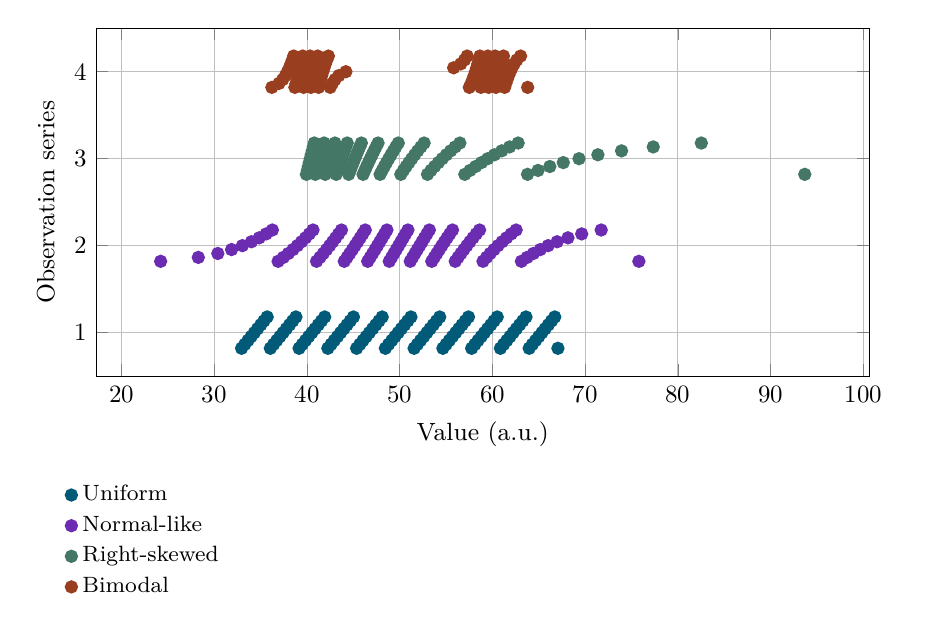
\begin{tikzpicture}
\begin{axis}[width=0.94\linewidth,
height=6cm,
scale only axis=false,
grid=major,
tick label style={font=\small},
label style={font=\small},
xlabel={Value (a.u.)},
ylabel={Observation series},
legend style={font=\footnotesize,draw=none,at={(0.5,-0.28)},anchor=north,legend columns=1,text width=0.85\linewidth,align=left},
unbounded coords=jump,
scaled ticks=false,
ymin=0.5,
ymax=4.5]
\addplot[color=pcd1,thick,only marks,mark=*] coordinates {(32.937795808244,0.8200000000000001) (33.282486802016,0.865) (33.627177795789,0.91) (33.971868789562,0.955) (34.316559783335,1) (34.661250777108,1.045) (35.005941770881,1.09) (35.350632764654,1.135) (35.695323758426,1.18) (36.040014752199,0.8200000000000001) (36.384705745972,0.865) (36.729396739745,0.91) (37.074087733518,0.955) (37.418778727291,1) (37.763469721064,1.045) (38.108160714836,1.09) (38.452851708609,1.135) (38.797542702382,1.18) (39.142233696155,0.8200000000000001) (39.486924689928,0.865) (39.831615683701,0.91) (40.176306677474,0.955) (40.520997671246,1) (40.865688665019,1.045) (41.210379658792,1.09) (41.555070652565,1.135) (41.899761646338,1.18) (42.244452640111,0.8200000000000001) (42.589143633884,0.865) (42.933834627656,0.91) (43.278525621429,0.955) (43.623216615202,1) (43.967907608975,1.045) (44.312598602748,1.09) (44.657289596521,1.135) (45.001980590294,1.18) (45.346671584066,0.8200000000000001) (45.691362577839,0.865) (46.036053571612,0.91) (46.380744565385,0.955) (46.725435559158,1) (47.070126552931,1.045) (47.414817546704,1.09) (47.759508540476,1.135) (48.104199534249,1.18) (48.448890528022,0.8200000000000001) (48.793581521795,0.865) (49.138272515568,0.91) (49.482963509341,0.955) (49.827654503114,1) (50.172345496886,1.045) (50.517036490659,1.09) (50.861727484432,1.135) (51.206418478205,1.18) (51.551109471978,0.8200000000000001) (51.895800465751,0.865) (52.240491459524,0.91) (52.585182453296,0.955) (52.929873447069,1) (53.274564440842,1.045) (53.619255434615,1.09) (53.963946428388,1.135) (54.308637422161,1.18) (54.653328415934,0.8200000000000001) (54.998019409706,0.865) (55.342710403479,0.91) (55.687401397252,0.955) (56.032092391025,1) (56.376783384798,1.045) (56.721474378571,1.09) (57.066165372344,1.135) (57.410856366116,1.18) (57.755547359889,0.8200000000000001) (58.100238353662,0.865) (58.444929347435,0.91) (58.789620341208,0.955) (59.134311334981,1) (59.479002328754,1.045) (59.823693322526,1.09) (60.168384316299,1.135) (60.513075310072,1.18) (60.857766303845,0.8200000000000001) (61.202457297618,0.865) (61.547148291391,0.91) (61.891839285164,0.955) (62.236530278936,1) (62.581221272709,1.045) (62.925912266482,1.09) (63.270603260255,1.135) (63.615294254028,1.18) (63.959985247801,0.8200000000000001) (64.304676241574,0.865) (64.649367235346,0.91) (64.994058229119,0.955) (65.338749222892,1) (65.683440216665,1.045) (66.028131210438,1.09) (66.372822204211,1.135) (66.717513197983,1.18) (67.062204191756,0.8200000000000001)};
\addlegendentry{Uniform}
\addplot[color=pcd2,thick,only marks,mark=*] coordinates {(24.206635835883,1.82) (28.269549422019,1.865) (30.373674322229,1.91) (31.856223253642,1.955) (33.022939259286,2) (33.996308448767,2.045) (34.838365913792,2.09) (35.58508539193,2.135) (36.259278709141,2.18) (36.876364726706,1.82) (37.447277731692,1.865) (37.980067968729,1.91) (38.48084364786,1.955) (38.954355721997,2) (39.40437699918,2.045) (39.833956941897,2.09) (40.245598210373,2.135) (40.641382216077,2.18) (41.023060453084,1.82) (41.392122262472,1.865) (41.749845996961,1.91) (42.097338257528,1.955) (42.435564405174,2) (42.765372588295,2.045) (43.087512881045,2.09) (43.402652687281,2.135) (43.711389258082,2.18) (44.014259954043,1.82) (44.31175072803,1.865) (44.604303190988,1.91) (44.892320540063,1.955) (45.176172566306,2) (45.456199912458,2.045) (45.732717715837,2.09) (46.006018744083,2.135) (46.276376110428,2.18) (46.544045638705,1.82) (46.809267935405,1.865) (47.072270215874,1.91) (47.333267923585,1.955) (47.592466174974,2) (47.850061057056,2.045) (48.106240800864,2.09) (48.361186850331,2.135) (48.615074843483,2.18) (48.868075520607,1.82) (49.120355572217,1.865) (49.372078438265,1.91) (49.623405068846,1.955) (49.874494655831,2) (50.125505344169,2.045) (50.376594931154,2.09) (50.627921561735,2.135) (50.879644427783,2.18) (51.131924479393,1.82) (51.384925156517,1.865) (51.638813149669,1.91) (51.893759199136,1.955) (52.149938942944,2) (52.407533825026,2.045) (52.666732076415,2.09) (52.927729784126,2.135) (53.190732064595,2.18) (53.455954361295,1.82) (53.723623889572,1.865) (53.993981255917,1.91) (54.267282284163,1.955) (54.543800087542,2) (54.823827433694,2.045) (55.107679459937,2.09) (55.395696809012,2.135) (55.68824927197,2.18) (55.985740045957,1.82) (56.288610741918,1.865) (56.597347312719,1.91) (56.912487118955,1.955) (57.234627411705,2) (57.564435594826,2.045) (57.902661742472,2.09) (58.250154003039,2.135) (58.607877737528,2.18) (58.976939546916,1.82) (59.358617783923,1.865) (59.754401789627,1.91) (60.166043058103,1.955) (60.59562300082,2) (61.045644278003,2.045) (61.51915635214,2.09) (62.019932031271,2.135) (62.552722268308,2.18) (63.123635273294,1.82) (63.740721290859,1.865) (64.41491460807,1.91) (65.161634086208,1.955) (66.003691551233,2) (66.977060740714,2.045) (68.143776746358,2.09) (69.626325677771,2.135) (71.730450577981,2.18) (75.793364164117,1.82)};
\addlegendentry{Normal-like}
\addplot[color=pcd3,thick,only marks,mark=*] coordinates {(39.930215496246,2.82) (40.032800674276,2.865) (40.136432657911,2.91) (40.24113303134,2.955) (40.346924053282,3) (40.453828685386,3.045) (40.56187062215,3.09) (40.671074322438,3.135) (40.781465042716,3.18) (40.893068872116,2.82) (41.00591276944,2.865) (41.120024602253,2.91) (41.235433188192,2.955) (41.352168338646,3) (41.470260904983,3.045) (41.589742827495,3.09) (41.710647187247,3.135) (41.833008261065,3.18) (41.956861579865,2.82) (42.082243990591,2.865) (42.209193722015,2.91) (42.337750454712,2.955) (42.467955395514,3) (42.599851356805,3.045) (42.733482841024,3.09) (42.868896130814,3.135) (43.00613938525,3.18) (43.145262742673,2.82) (43.286318430648,2.865) (43.429360883685,2.91) (43.574446869357,2.955) (43.721635623558,3) (43.870988995719,3.045) (44.022571604848,3.09) (44.176451007399,3.135) (44.332697878059,3.18) (44.491386204653,2.82) (44.652593498525,2.865) (44.816401021887,2.91) (44.982894033802,2.955) (45.152162056669,3) (45.324299165303,3.045) (45.499404300925,3.09) (45.677581612709,3.135) (45.85894082983,3.18) (46.043597667329,2.82) (46.23167426958,2.865) (46.423299695584,2.91) (46.618610450948,2.955) (46.817751072022,3) (47.020874768457,3.045) (47.228144131353,3.09) (47.439731915181,3.135) (47.655821902906,3.18) (47.876609865167,2.82) (48.102304626062,2.865) (48.333129250065,2.91) (48.569322367003,2.955) (48.811139654802,3) (49.058855503111,3.045) (49.31276488494,3.09) (49.573185468321,3.135) (49.840460005917,3.18) (50.114959047658,2.82) (50.397084030267,2.865) (50.687270808317,2.91) (50.98599370477,2.955) (51.293770175501,3) (51.611166202976,3.045) (51.938802560306,3.09) (52.277362119843,3.135) (52.627598422573,3.18) (52.990345778654,2.82) (53.366531239605,2.865) (53.757188874395,2.91) (54.16347690284,2.955) (54.586698401275,3) (55.028326513309,3.045) (55.490035395649,3.09) (55.973738539477,3.135) (56.481636682893,3.18) (57.016278347419,2.82) (57.580637213174,2.865) (58.178212286046,2.91) (58.813159420496,2.955) (59.490466767655,3) (60.216193020701,3.045) (60.997797523507,3.09) (61.844608325906,3.135) (62.768503720566,3.18) (63.784935940163,2.82) (64.914526391984,2.865) (66.185664030899,2.91) (67.638974200483,2.955) (69.335549803636,3) (71.373530538291,3.045) (73.925841238155,3.09) (77.343001548489,3.135) (82.530868055881,3.18) (93.688205573471,2.82)};
\addlegendentry{Right-skewed}
\addplot[color=pcd4,thick,only marks,mark=*] coordinates {(36.203861904595,3.82) (36.968344965996,3.865) (37.373171342811,3.91) (37.663249348955,3.955) (37.894944427129,4) (38.090935235275,4.045) (38.26275052086,4.09) (38.417100222768,4.135) (38.558256085355,4.18) (38.689118543731,3.82) (38.811755599904,3.865) (38.927699911254,3.91) (39.038123973652,3.955) (39.143949102676,4) (39.245916271163,4.045) (39.344633882841,4.09) (39.44061103123,4.135) (39.534281313527,4.18) (39.626020324213,3.82) (39.716158820762,3.865) (39.804992871389,3.91) (39.892791871197,3.955) (39.979805043931,4) (40.066266872452,4.045) (40.152401787581,4.09) (40.238428371541,4.135) (40.324563286669,4.18) (40.411025115191,3.82) (40.498038287925,3.865) (40.585837287733,3.91) (40.674671338359,3.955) (40.764809834908,4) (40.856548845594,4.045) (40.950219127892,4.09) (41.04619627628,4.135) (41.144913887958,4.18) (41.246881056446,3.82) (41.352706185469,3.865) (41.463130247867,3.91) (41.579074559217,3.955) (41.70171161539,4) (41.832574073766,4.045) (41.973729936353,4.09) (42.128079638261,4.135) (42.299894923847,4.18) (42.495885731992,3.82) (42.727580810167,3.865) (43.01765881631,3.91) (43.422485193125,3.955) (44.186968254526,4) (55.813031745474,4.045) (56.577514806875,4.09) (56.98234118369,4.135) (57.272419189833,4.18) (57.504114268008,3.82) (57.700105076153,3.865) (57.871920361739,3.91) (58.026270063647,3.955) (58.167425926234,4) (58.29828838461,4.045) (58.420925440783,4.09) (58.536869752133,4.135) (58.647293814531,4.18) (58.753118943554,3.82) (58.855086112042,3.865) (58.95380372372,3.91) (59.049780872108,3.955) (59.143451154406,4) (59.235190165092,4.045) (59.325328661641,4.09) (59.414162712267,4.135) (59.501961712075,4.18) (59.588974884809,3.82) (59.675436713331,3.865) (59.761571628459,3.91) (59.847598212419,3.955) (59.933733127548,4) (60.020194956069,4.045) (60.107208128803,4.09) (60.195007128611,4.135) (60.283841179238,4.18) (60.373979675787,3.82) (60.465718686473,3.865) (60.55938896877,3.91) (60.655366117159,3.955) (60.754083728837,4) (60.856050897324,4.045) (60.961876026348,4.09) (61.072300088746,4.135) (61.188244400096,4.18) (61.310881456269,3.82) (61.441743914645,3.865) (61.582899777232,3.91) (61.73724947914,3.955) (61.909064764725,4) (62.105055572871,4.045) (62.336750651045,4.09) (62.626828657189,4.135) (63.031655034004,4.18) (63.796138095405,3.82)};
\addlegendentry{Bimodal}

\end{axis}
\end{tikzpicture}
\end{center}

\medskip

The data notation in \hyperref[material-8aaa7b1410a5e1c052f99d382f23cdcba6eb2964bb0e8445f7f605705af8be9a]{Eq.~\ref*{material-8aaa7b1410a5e1c052f99d382f23cdcba6eb2964bb0e8445f7f605705af8be9a}} identifies the sample, and the order-statistic notation in \hyperref[material-6b73f7f64eb95e9e5cda839029d58b14bae7aa599b27037a427dd204a2930350]{Eq.~\ref*{material-6b73f7f64eb95e9e5cda839029d58b14bae7aa599b27037a427dd204a2930350}} assigns ranks after sorting. The range (\hyperref[material-8f9d95106361e7a359ea1c0893e2c80e9585bda6c2f983c97a0b2a706452e7fd]{Eq.~\ref*{material-8f9d95106361e7a359ea1c0893e2c80e9585bda6c2f983c97a0b2a706452e7fd}}) describes the distance between the observed endpoints. Because those endpoints are individual observations, their behaviour depends strongly on sample size and on extreme values. This makes the range useful as an observed extent with an explicitly stated sampling context.


\par\medskip
\noindent\begin{minipage}{\linewidth}
\refstepcounter{equation}\label{material-8aaa7b1410a5e1c052f99d382f23cdcba6eb2964bb0e8445f7f605705af8be9a}
\noindent\textbf{Eq.~\ref*{material-8aaa7b1410a5e1c052f99d382f23cdcba6eb2964bb0e8445f7f605705af8be9a}.} Sample notation with observation identity, sample size and quantity conventions.\par\nopagebreak
\begin{center}\begin{adjustbox}{max width=\linewidth}$\displaystyle \begin{gathered}x_1,\ldots,x_n,\qquad n=5\\(10.2,\ 9.8,\ 10.0,\ 10.0,\ 10.1)\;\mathrm{mg/L}\end{gathered}$\end{adjustbox}\end{center}

\par\noindent\textbf{Symbols}

\par\noindent\textbf{What does i identify?} i labels the observation in acquisition order, not its rank. n counts all readings, including ties. Synthetic teaching data.

\end{minipage}\par
\medskip

\par\medskip
\noindent\begin{minipage}{\linewidth}
\refstepcounter{equation}\label{material-6b73f7f64eb95e9e5cda839029d58b14bae7aa599b27037a427dd204a2930350}
\noindent\textbf{Eq.~\ref*{material-6b73f7f64eb95e9e5cda839029d58b14bae7aa599b27037a427dd204a2930350}.} Ordered-observation notation with rank and tie conventions explained.\par\nopagebreak
\begin{center}\begin{adjustbox}{max width=\linewidth}$\displaystyle \begin{gathered}(x_1,\ldots,x_5)=(10.2,9.8,10.0,10.0,10.1)\\x_{(1)}\le\cdots\le x_{(5)}\\(x_{(1)},\ldots,x_{(5)})=(9.8,10.0,10.0,10.1,10.2)\end{gathered}$\end{adjustbox}\end{center}

\par\noindent\textbf{Symbols}

\par\noindent\textbf{Same values, different meaning of the index} All values are in mg/L. x\ensuremath{{}_1}=10.2, but x\ensuremath{{}_{(}}\ensuremath{{}_1}\ensuremath{{}_{)}}=9.8 is the minimum. x\ensuremath{{}_{(}}\ensuremath{{}_2}\ensuremath{{}_{)}}=x\ensuremath{{}_{(}}\ensuremath{{}_3}\ensuremath{{}_{)}}=10.0: two observations, not one. x\ensuremath{{}_{(}}\ensuremath{{}_n}\ensuremath{{}_{)}} is the maximum.

\end{minipage}\par
\medskip

\par\medskip
\noindent\begin{minipage}{\linewidth}
\refstepcounter{equation}\label{material-8f9d95106361e7a359ea1c0893e2c80e9585bda6c2f983c97a0b2a706452e7fd}
\noindent\textbf{Eq.~\ref*{material-8f9d95106361e7a359ea1c0893e2c80e9585bda6c2f983c97a0b2a706452e7fd}.} Observed range as the difference between the largest and smallest values.\par\nopagebreak
\begin{center}\begin{adjustbox}{max width=\linewidth}$\displaystyle R=x_{(n)}-x_{(1)},\qquad n\ge1$\end{adjustbox}\end{center}

\par\noindent\textbf{Symbols}

\par\noindent\textbf{Order first} x\ensuremath{{}_{(}}\ensuremath{{}_1}\ensuremath{{}_{)}} is the minimum; x\ensuremath{{}_{(}}\ensuremath{{}_n}\ensuremath{{}_{)}} is the maximum. R is a width, not the endpoint pair returned by R's range(x).

\end{minipage}\par
\medskip

Quartiles and other quantiles describe locations within the ordered collection. The quartile construction in \hyperref[material-834e4fa62bba03712f873886a6bff8a9e68880e3d2fe07bd99b1c17e27727569]{Eq.~\ref*{material-834e4fa62bba03712f873886a6bff8a9e68880e3d2fe07bd99b1c17e27727569}} and the interpolation rule in \hyperref[material-b3a97c9104cdf8ff9365bac8ad880885cdeacfa96c9d2a0f38e0973715c30043]{Eq.~\ref*{material-b3a97c9104cdf8ff9365bac8ad880885cdeacfa96c9d2a0f38e0973715c30043}} make the chosen finite-sample convention reproducible. The application in \hyperref[material-402e28d5ca82eecc9de8c8753e265dcf1d2dd6b4b7aa3d3d26caa5f1f9a41348]{Fig.~\ref*{material-402e28d5ca82eecc9de8c8753e265dcf1d2dd6b4b7aa3d3d26caa5f1f9a41348}} connects a selected probability level with a concentration threshold. Reporting the convention is particularly useful for small samples, where alternative accepted definitions can give visibly different answers.


\par\medskip
\noindent\begin{minipage}{\linewidth}
\refstepcounter{equation}\label{material-834e4fa62bba03712f873886a6bff8a9e68880e3d2fe07bd99b1c17e27727569}
\noindent\textbf{Eq.~\ref*{material-834e4fa62bba03712f873886a6bff8a9e68880e3d2fe07bd99b1c17e27727569}.} Authored quartile-position convention and its interpolation notation.\par\nopagebreak
\begin{center}\begin{adjustbox}{max width=\linewidth}$\displaystyle Q_1=\widehat Q(0.25),\quad Q_2=\widehat Q(0.50),\quad Q_3=\widehat Q(0.75)$\end{adjustbox}\end{center}

\par\noindent\textbf{Symbols}

\par\noindent\textbf{Quarter, half, three quarters} Q\ensuremath{{}_1}, Q\ensuremath{{}_2} and Q\ensuremath{{}_3} are the lower quartile, sample median and upper quartile. Q̂(p) is the linearly interpolated sample quantile at cumulative proportion p. The fractions 0.25, 0.50 and 0.75 are unitless; all quantile values have the measurement unit.

\end{minipage}\par
\medskip

\par\medskip
\noindent\begin{minipage}{\linewidth}
\refstepcounter{equation}\label{material-b3a97c9104cdf8ff9365bac8ad880885cdeacfa96c9d2a0f38e0973715c30043}
\noindent\textbf{Eq.~\ref*{material-b3a97c9104cdf8ff9365bac8ad880885cdeacfa96c9d2a0f38e0973715c30043}.} Finite-sample quantile interpolation with the complete probability, rank and endpoint conventions.\par\nopagebreak
\begin{center}\begin{adjustbox}{max width=\linewidth}$\displaystyle \begin{gathered}h=1+(n-1)p,\quad j=\lfloor h\rfloor,\quad d=h-j\\\widehat Q(p)=(1-d)x_{(j)}+d\,x_{(j+1)}\\ n\ge2,\quad 0\le p<1\end{gathered}$\end{adjustbox}\end{center}

\par\noindent\textbf{Symbols}

\par\noindent\textbf{Interpolate between adjacent ranks} p: unitless cumulative proportion; n: number of observations; h: fractional rank; floor(h): round h down to integer j; d: unitless interpolation weight h\ensuremath{-}j. x\ensuremath{{}_{(}}\ensuremath{{}_j}\ensuremath{{}_{)}} and x\ensuremath{{}_{(}}\ensuremath{{}_j}\ensuremath{{}_+}\ensuremath{{}_1}\ensuremath{{}_{)}} are adjacent ordered values; Q̂(p) is their weighted average, in the measurement unit. The factors 1\ensuremath{-}d and d sum to one. The displayed interior case requires n\ensuremath{\ge}2 and p<1; at p=1 return the maximum, and for n=1 return the sole observation.

\end{minipage}\par
\medskip

\par\medskip
\Needspace{10cm}
\refstepcounter{figure}\label{material-402e28d5ca82eecc9de8c8753e265dcf1d2dd6b4b7aa3d3d26caa5f1f9a41348}
\noindent\textbf{Fig.~\ref*{material-402e28d5ca82eecc9de8c8753e265dcf1d2dd6b4b7aa3d3d26caa5f1f9a41348}.} Authored quantile application linking an ordered concentration sample with selected cumulative levels.\par\nopagebreak
\begin{center}
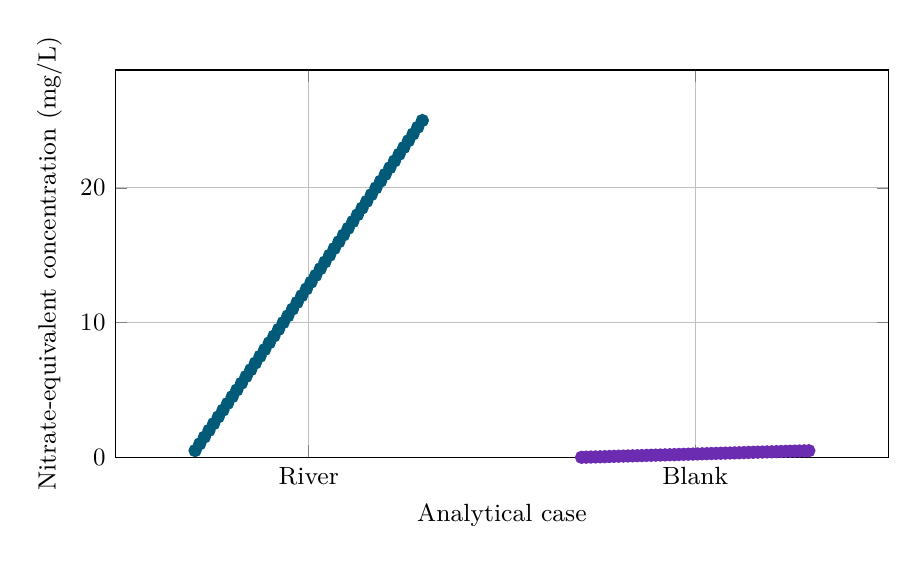
\begin{tikzpicture}
\begin{axis}[width=0.94\linewidth,
height=6.5cm,
scale only axis=false,
grid=major,
tick label style={font=\small},
label style={font=\small},
xlabel={Analytical case},
ylabel={Nitrate-equivalent concentration (mg/L)},
legend style={font=\footnotesize,draw=none,at={(0.5,-0.28)},anchor=north,legend columns=1,text width=0.85\linewidth,align=left},
unbounded coords=jump,
scaled ticks=false,
ymin=0,
ymax=28.75,
xmin=0.5,
xmax=2.5,
xtick={1,2},
xticklabels={{River},{Blank}}]
\addplot[color=pcd1,thick,only marks,mark=*] coordinates {(0.706,0.5) (0.718,1) (0.73,1.5) (0.742,2) (0.754,2.5) (0.766,3) (0.778,3.5) (0.79,4) (0.802,4.5) (0.8140000000000001,5) (0.826,5.5) (0.838,6) (0.85,6.5) (0.862,7) (0.874,7.5) (0.886,8) (0.898,8.5) (0.91,9) (0.922,9.5) (0.9339999999999999,10) (0.946,10.5) (0.958,11) (0.97,11.5) (0.982,12) (0.994,12.5) (1.006,13) (1.018,13.5) (1.03,14) (1.042,14.5) (1.054,15) (1.066,15.5) (1.078,16) (1.09,16.5) (1.102,17) (1.114,17.5) (1.126,18) (1.138,18.5) (1.15,19) (1.162,19.5) (1.174,20) (1.186,20.5) (1.198,21) (1.21,21.5) (1.222,22) (1.234,22.5) (1.246,23) (1.258,23.5) (1.27,24) (1.282,24.5) (1.294,25)};
\addplot[color=pcd2,thick,only marks,mark=*] coordinates {(1.706,0) (1.718,0.01) (1.73,0.02) (1.742,0.03) (1.754,0.04) (1.766,0.05) (1.778,0.06) (1.79,0.07) (1.802,0.08) (1.814,0.09) (1.826,0.1) (1.838,0.11) (1.85,0.12) (1.862,0.13) (1.874,0.14) (1.886,0.15) (1.898,0.16) (1.91,0.17) (1.922,0.18) (1.934,0.19) (1.946,0.2) (1.958,0.21) (1.97,0.22) (1.982,0.23) (1.994,0.24) (2.006,0.25) (2.018,0.26) (2.03,0.27) (2.042,0.28) (2.054,0.29) (2.066,0.3) (2.078,0.31) (2.09,0.32) (2.102,0.33) (2.114,0.34) (2.126,0.35) (2.138,0.36) (2.15,0.37) (2.162,0.38) (2.174,0.39) (2.186,0.4) (2.198,0.41) (2.21,0.42) (2.222,0.43) (2.234,0.44) (2.246,0.45) (2.258,0.46) (2.27,0.47) (2.282,0.48) (2.294,0.49)};

\end{axis}
\end{tikzpicture}
\end{center}


\medskip

\clearpage
\section{Choose a spread summary for the part of the distribution of interest}
A spread measure emphasizes particular features of the observations. The interquartile range in \hyperref[material-1efd475ee0eb348a412dcda5c00354f2a64c89157908b599d6ce36af59720dd5]{Eq.~\ref*{material-1efd475ee0eb348a412dcda5c00354f2a64c89157908b599d6ce36af59720dd5}} measures the distance from the lower quartile to the upper quartile. Its application in \hyperref[material-ddec8a09c6ab106cd1e41f709c2067338f031f59e8d4d06d742df0867a96ca5b]{Fig.~\ref*{material-ddec8a09c6ab106cd1e41f709c2067338f031f59e8d4d06d742df0867a96ca5b}} describes the central half of the ordered data using the authored quantile convention. The tail comparison in \hyperref[material-fd009b41e07bde16906a9a0f48161c6b4499ff4c718e3b95e42f6737cde96b70]{Fig.~\ref*{material-fd009b41e07bde16906a9a0f48161c6b4499ff4c718e3b95e42f6737cde96b70}} shows why we retain tail observations alongside this central summary.


\par\medskip
\noindent\begin{minipage}{\linewidth}
\refstepcounter{equation}\label{material-1efd475ee0eb348a412dcda5c00354f2a64c89157908b599d6ce36af59720dd5}
\noindent\textbf{Eq.~\ref*{material-1efd475ee0eb348a412dcda5c00354f2a64c89157908b599d6ce36af59720dd5}.} Interquartile range in the original measurement unit, using the authored quartile convention.\par\nopagebreak
\begin{center}\begin{adjustbox}{max width=\linewidth}$\displaystyle \mathrm{IQR}(x_1,\ldots,x_n)=\widehat Q(0.75)-\widehat Q(0.25),\quad n\ge1$\end{adjustbox}\end{center}

\par\noindent\textbf{Symbols}

\par\noindent\textbf{A width in the original unit} x\ensuremath{{}_1},\ensuremath{\ldots},x\ensuremath{{}_n}: observed values; n\ensuremath{\ge}1: sample size. Q̂(p): linearly interpolated sample quantile at unitless proportion p. Subtract the lower quartile at 0.25 from the upper quartile at 0.75. IQR is this central width in the measurement unit, not the entire observed range.

\end{minipage}\par
\medskip

\par\medskip
\Needspace{10cm}
\refstepcounter{figure}\label{material-ddec8a09c6ab106cd1e41f709c2067338f031f59e8d4d06d742df0867a96ca5b}
\noindent\textbf{Fig.~\ref*{material-ddec8a09c6ab106cd1e41f709c2067338f031f59e8d4d06d742df0867a96ca5b}.} Authored IQR application showing the separation of the lower and upper quartiles.\par\nopagebreak
\begin{center}
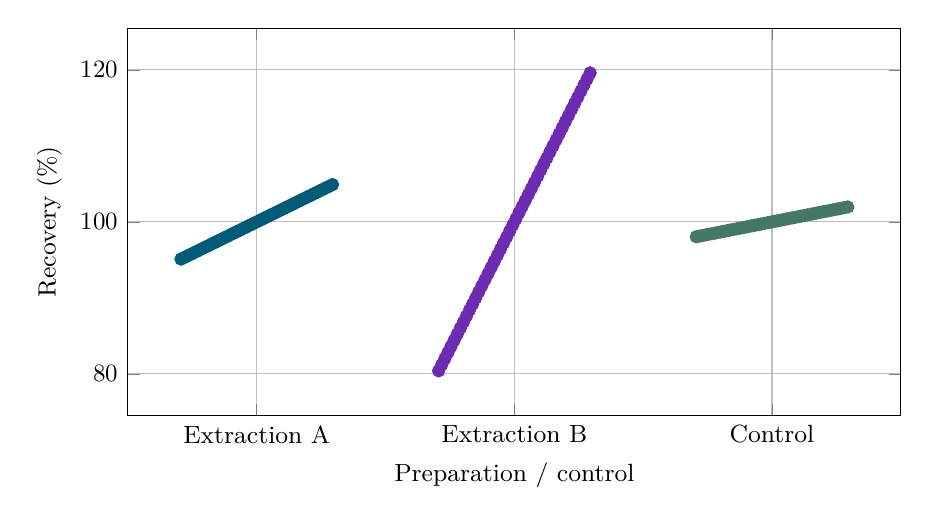
\begin{tikzpicture}
\begin{axis}[width=0.94\linewidth,
height=6.5cm,
scale only axis=false,
grid=major,
tick label style={font=\small},
label style={font=\small},
xlabel={Preparation / control},
ylabel={Recovery (\%)},
legend style={font=\footnotesize,draw=none,at={(0.5,-0.28)},anchor=north,legend columns=1,text width=0.85\linewidth,align=left},
unbounded coords=jump,
scaled ticks=false,
ymin=74.52000000000001,
ymax=125.47999999999999,
xmin=0.5,
xmax=3.5,
xtick={1,2,3},
xticklabels={{Extraction A},{Extraction B},{Control}}]
\addplot[color=pcd1,thick,only marks,mark=*] coordinates {(0.706,95.1) (0.718,95.3) (0.73,95.5) (0.742,95.7) (0.754,95.9) (0.766,96.1) (0.778,96.3) (0.79,96.5) (0.802,96.7) (0.8140000000000001,96.9) (0.826,97.1) (0.838,97.3) (0.85,97.5) (0.862,97.7) (0.874,97.9) (0.886,98.1) (0.898,98.3) (0.91,98.5) (0.922,98.7) (0.9339999999999999,98.9) (0.946,99.1) (0.958,99.3) (0.97,99.5) (0.982,99.7) (0.994,99.9) (1.006,100.1) (1.018,100.3) (1.03,100.5) (1.042,100.7) (1.054,100.9) (1.066,101.1) (1.078,101.3) (1.09,101.5) (1.102,101.7) (1.114,101.9) (1.126,102.1) (1.138,102.3) (1.15,102.5) (1.162,102.7) (1.174,102.9) (1.186,103.1) (1.198,103.3) (1.21,103.5) (1.222,103.7) (1.234,103.9) (1.246,104.1) (1.258,104.3) (1.27,104.5) (1.282,104.7) (1.294,104.9)};
\addplot[color=pcd2,thick,only marks,mark=*] coordinates {(1.706,80.4) (1.718,81.2) (1.73,82) (1.742,82.8) (1.754,83.6) (1.766,84.4) (1.778,85.2) (1.79,86) (1.802,86.8) (1.814,87.6) (1.826,88.4) (1.838,89.2) (1.85,90) (1.862,90.8) (1.874,91.6) (1.886,92.4) (1.898,93.2) (1.91,94) (1.922,94.8) (1.934,95.6) (1.946,96.4) (1.958,97.2) (1.97,98) (1.982,98.8) (1.994,99.6) (2.006,100.4) (2.018,101.2) (2.03,102) (2.042,102.8) (2.054,103.6) (2.066,104.4) (2.078,105.2) (2.09,106) (2.102,106.8) (2.114,107.6) (2.126,108.4) (2.138,109.2) (2.15,110) (2.162,110.8) (2.174,111.6) (2.186,112.4) (2.198,113.2) (2.21,114) (2.222,114.8) (2.234,115.6) (2.246,116.4) (2.258,117.2) (2.27,118) (2.282,118.8) (2.294,119.6)};
\addplot[color=pcd3,thick,only marks,mark=*] coordinates {(2.706,98.04) (2.718,98.12) (2.73,98.2) (2.742,98.28) (2.754,98.36) (2.766,98.44) (2.778,98.52) (2.79,98.6) (2.802,98.68) (2.814,98.76) (2.826,98.84) (2.838,98.92) (2.85,99) (2.862,99.08) (2.874,99.16) (2.886,99.24) (2.898,99.32) (2.91,99.4) (2.922,99.48) (2.934,99.56) (2.946,99.64) (2.958,99.72) (2.97,99.8) (2.982,99.88) (2.994,99.96) (3.006,100.04) (3.018,100.12) (3.03,100.2) (3.042,100.28) (3.054,100.36) (3.066,100.44) (3.078,100.52) (3.09,100.6) (3.102,100.68) (3.114,100.76) (3.126,100.84) (3.138,100.92) (3.15,101) (3.162,101.08) (3.174,101.16) (3.186,101.24) (3.198,101.32) (3.21,101.4) (3.222,101.48) (3.234,101.56) (3.246,101.64) (3.258,101.72) (3.27,101.8) (3.282,101.88) (3.294,101.96)};

\end{axis}
\end{tikzpicture}
\end{center}


\medskip

\par\medskip
\Needspace{10cm}
\refstepcounter{figure}\label{material-fd009b41e07bde16906a9a0f48161c6b4499ff4c718e3b95e42f6737cde96b70}
\noindent\textbf{Fig.~\ref*{material-fd009b41e07bde16906a9a0f48161c6b4499ff4c718e3b95e42f6737cde96b70}.} Tail comparison accompanying the IQR: central quartile separation is read together with the extreme observations.\par\nopagebreak
\begin{center}
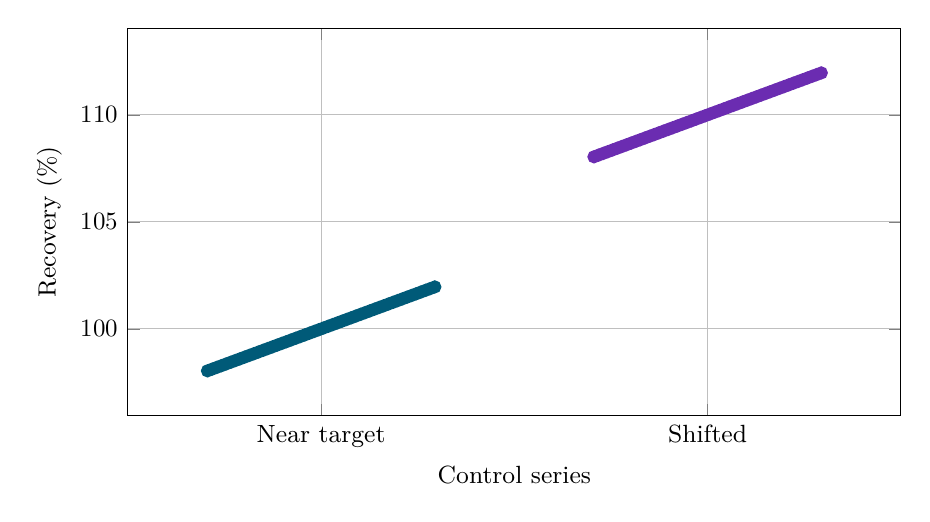
\begin{tikzpicture}
\begin{axis}[width=0.94\linewidth,
height=6.5cm,
scale only axis=false,
grid=major,
tick label style={font=\small},
label style={font=\small},
xlabel={Control series},
ylabel={Recovery (\%)},
legend style={font=\footnotesize,draw=none,at={(0.5,-0.28)},anchor=north,legend columns=1,text width=0.85\linewidth,align=left},
unbounded coords=jump,
scaled ticks=false,
ymin=95.95200000000001,
ymax=114.04799999999999,
xmin=0.5,
xmax=2.5,
xtick={1,2},
xticklabels={{Near target},{Shifted}}]
\addplot[color=pcd1,thick,only marks,mark=*] coordinates {(0.706,98.04) (0.718,98.12) (0.73,98.2) (0.742,98.28) (0.754,98.36) (0.766,98.44) (0.778,98.52) (0.79,98.6) (0.802,98.68) (0.8140000000000001,98.76) (0.826,98.84) (0.838,98.92) (0.85,99) (0.862,99.08) (0.874,99.16) (0.886,99.24) (0.898,99.32) (0.91,99.4) (0.922,99.48) (0.9339999999999999,99.56) (0.946,99.64) (0.958,99.72) (0.97,99.8) (0.982,99.88) (0.994,99.96) (1.006,100.04) (1.018,100.12) (1.03,100.2) (1.042,100.28) (1.054,100.36) (1.066,100.44) (1.078,100.52) (1.09,100.6) (1.102,100.68) (1.114,100.76) (1.126,100.84) (1.138,100.92) (1.15,101) (1.162,101.08) (1.174,101.16) (1.186,101.24) (1.198,101.32) (1.21,101.4) (1.222,101.48) (1.234,101.56) (1.246,101.64) (1.258,101.72) (1.27,101.8) (1.282,101.88) (1.294,101.96)};
\addplot[color=pcd2,thick,only marks,mark=*] coordinates {(1.706,108.04) (1.718,108.12) (1.73,108.2) (1.742,108.28) (1.754,108.36) (1.766,108.44) (1.778,108.52) (1.79,108.6) (1.802,108.68) (1.814,108.76) (1.826,108.84) (1.838,108.92) (1.85,109) (1.862,109.08) (1.874,109.16) (1.886,109.24) (1.898,109.32) (1.91,109.4) (1.922,109.48) (1.934,109.56) (1.946,109.64) (1.958,109.72) (1.97,109.8) (1.982,109.88) (1.994,109.96) (2.006,110.04) (2.018,110.12) (2.03,110.2) (2.042,110.28) (2.054,110.36) (2.066,110.44) (2.078,110.52) (2.09,110.6) (2.102,110.68) (2.114,110.76) (2.126,110.84) (2.138,110.92) (2.15,111) (2.162,111.08) (2.174,111.16) (2.186,111.24) (2.198,111.32) (2.21,111.4) (2.222,111.48) (2.234,111.56) (2.246,111.64) (2.258,111.72) (2.27,111.8) (2.282,111.88) (2.294,111.96)};

\end{axis}
\end{tikzpicture}
\end{center}


\medskip

The median absolute deviation first measures absolute distance from the median and then takes the median of those distances (\hyperref[material-4e7de599cebc337e378cc81970f07039c215b6cf32181fb7cf582a079c500001]{Eq.~\ref*{material-4e7de599cebc337e378cc81970f07039c215b6cf32181fb7cf582a079c500001}}). The worked application in \hyperref[material-ddae9ddfa47e94d75b2646a223d4ef63e892550f4f5a4f74f093fb6dd6fdcd53]{Fig.~\ref*{material-ddae9ddfa47e94d75b2646a223d4ef63e892550f4f5a4f74f093fb6dd6fdcd53}} makes this two-stage ordering explicit. The raw quantity has the original measurement unit. A scaled version additionally specifies the scaling constant and its reference distribution, so the reported name and convention identify which quantity was calculated.


\par\medskip
\noindent\begin{minipage}{\linewidth}
\refstepcounter{equation}\label{material-4e7de599cebc337e378cc81970f07039c215b6cf32181fb7cf582a079c500001}
\noindent\textbf{Eq.~\ref*{material-4e7de599cebc337e378cc81970f07039c215b6cf32181fb7cf582a079c500001}.} Median absolute deviation with its centring, absolute-value and scaling conventions.\par\nopagebreak
\begin{center}\begin{adjustbox}{max width=\linewidth}$\displaystyle \mathrm{MAD}_{\mathrm{raw}}=\mathrm{median}_i\left|x_i-\mathrm{median}_j(x_j)\right|$\end{adjustbox}\end{center}

\par\noindent\textbf{Symbols}

\par\noindent\textbf{Two median operations} First find the sample median; then find the median of all absolute distances to it. No squaring and no averaging of these distances.

\end{minipage}\par
\medskip

\par\medskip
\Needspace{10cm}
\refstepcounter{figure}\label{material-ddae9ddfa47e94d75b2646a223d4ef63e892550f4f5a4f74f093fb6dd6fdcd53}
\noindent\textbf{Fig.~\ref*{material-ddae9ddfa47e94d75b2646a223d4ef63e892550f4f5a4f74f093fb6dd6fdcd53}.} Authored MAD example illustrating absolute distances from the sample median.\par\nopagebreak
\begin{center}
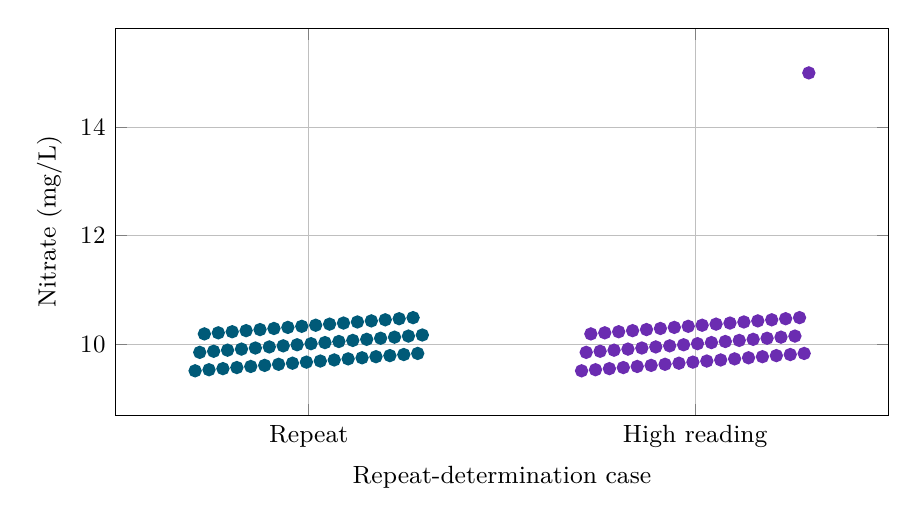
\begin{tikzpicture}
\begin{axis}[width=0.94\linewidth,
height=6.5cm,
scale only axis=false,
grid=major,
tick label style={font=\small},
label style={font=\small},
xlabel={Repeat-determination case},
ylabel={Nitrate (mg/L)},
legend style={font=\footnotesize,draw=none,at={(0.5,-0.28)},anchor=north,legend columns=1,text width=0.85\linewidth,align=left},
unbounded coords=jump,
scaled ticks=false,
ymin=8.6865,
ymax=15.8235,
xmin=0.5,
xmax=2.5,
xtick={1,2},
xticklabels={{Repeat},{High reading}}]
\addplot[color=pcd1,thick,only marks,mark=*] coordinates {(0.706,9.51) (0.718,9.85) (0.73,10.19) (0.742,9.53) (0.754,9.87) (0.766,10.21) (0.778,9.55) (0.79,9.89) (0.802,10.23) (0.8140000000000001,9.57) (0.826,9.91) (0.838,10.25) (0.85,9.59) (0.862,9.93) (0.874,10.27) (0.886,9.61) (0.898,9.95) (0.91,10.29) (0.922,9.63) (0.9339999999999999,9.97) (0.946,10.31) (0.958,9.65) (0.97,9.99) (0.982,10.33) (0.994,9.67) (1.006,10.01) (1.018,10.35) (1.03,9.69) (1.042,10.03) (1.054,10.37) (1.066,9.71) (1.078,10.05) (1.09,10.39) (1.102,9.73) (1.114,10.07) (1.126,10.41) (1.138,9.75) (1.15,10.09) (1.162,10.43) (1.174,9.77) (1.186,10.11) (1.198,10.45) (1.21,9.79) (1.222,10.13) (1.234,10.47) (1.246,9.81) (1.258,10.15) (1.27,10.49) (1.282,9.83) (1.294,10.17)};
\addplot[color=pcd2,thick,only marks,mark=*] coordinates {(1.706,9.51) (1.718,9.85) (1.73,10.19) (1.742,9.53) (1.754,9.87) (1.766,10.21) (1.778,9.55) (1.79,9.89) (1.802,10.23) (1.814,9.57) (1.826,9.91) (1.838,10.25) (1.85,9.59) (1.862,9.93) (1.874,10.27) (1.886,9.61) (1.898,9.95) (1.91,10.29) (1.922,9.63) (1.934,9.97) (1.946,10.31) (1.958,9.65) (1.97,9.99) (1.982,10.33) (1.994,9.67) (2.006,10.01) (2.018,10.35) (2.03,9.69) (2.042,10.03) (2.054,10.37) (2.066,9.71) (2.078,10.05) (2.09,10.39) (2.102,9.73) (2.114,10.07) (2.126,10.41) (2.138,9.75) (2.15,10.09) (2.162,10.43) (2.174,9.77) (2.186,10.11) (2.198,10.45) (2.21,9.79) (2.222,10.13) (2.234,10.47) (2.246,9.81) (2.258,10.15) (2.27,10.49) (2.282,9.83) (2.294,15)};

\end{axis}
\end{tikzpicture}
\end{center}


\medskip

Comparisons under the authored Normal and skewed examples (\hyperref[material-15db6966c5b0f32a16a5601ab7fcaa26f0469cd77b84d451898564bb537e22d1]{Fig.~\ref*{material-15db6966c5b0f32a16a5601ab7fcaa26f0469cd77b84d451898564bb537e22d1}}, \hyperref[material-1dad9bd5857a85547de1c11f63415c05eb5c5a3ce9f3e642c9f5944b566be174]{Fig.~\ref*{material-1dad9bd5857a85547de1c11f63415c05eb5c5a3ce9f3e642c9f5944b566be174}}) connect robust central spread with the overall shape. Standard deviation emphasizes squared departures; IQR emphasizes quartile separation; MAD emphasizes the typical absolute departure from the median. Choosing among them starts with the analytical question and the part of the distribution that carries the relevant information.


\par\medskip
\Needspace{10cm}
\refstepcounter{figure}\label{material-15db6966c5b0f32a16a5601ab7fcaa26f0469cd77b84d451898564bb537e22d1}
\noindent\textbf{Fig.~\ref*{material-15db6966c5b0f32a16a5601ab7fcaa26f0469cd77b84d451898564bb537e22d1}.} Spread summaries in the authored Normal reference example.\par\nopagebreak
\begin{center}
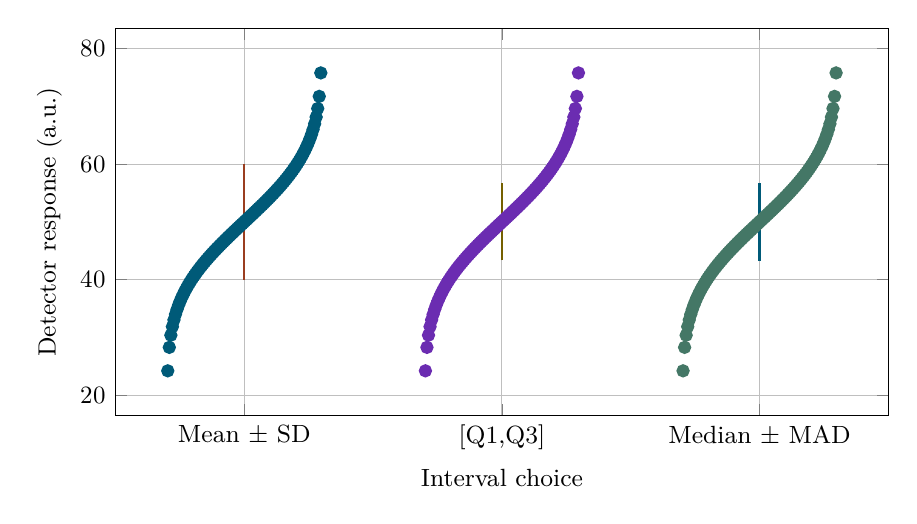
\begin{tikzpicture}
\begin{axis}[width=0.94\linewidth,
height=6.5cm,
scale only axis=false,
grid=major,
tick label style={font=\small},
label style={font=\small},
xlabel={Interval choice},
ylabel={Detector response (a.u.)},
legend style={font=\footnotesize,draw=none,at={(0.5,-0.28)},anchor=north,legend columns=1,text width=0.85\linewidth,align=left},
unbounded coords=jump,
scaled ticks=false,
ymin=16.4686265866479,
ymax=83.5313734133521,
xmin=0.5,
xmax=3.5,
xtick={1,2,3},
xticklabels={{Mean ± SD},{[Q1,Q3]},{Median ± MAD}}]
\addplot[color=pcd1,thick,only marks,mark=*] coordinates {(0.7030000000000001,24.206635835883) (0.7090000000000001,28.269549422019) (0.715,30.373674322229) (0.721,31.856223253642) (0.727,33.022939259286) (0.733,33.996308448767) (0.739,34.838365913792) (0.745,35.58508539193) (0.751,36.259278709141) (0.757,36.876364726706) (0.763,37.447277731692) (0.769,37.980067968729) (0.775,38.48084364786) (0.781,38.954355721997) (0.787,39.40437699918) (0.7929999999999999,39.833956941897) (0.7989999999999999,40.245598210373) (0.8049999999999999,40.641382216077) (0.8109999999999999,41.023060453084) (0.817,41.392122262472) (0.823,41.749845996961) (0.829,42.097338257528) (0.835,42.435564405174) (0.841,42.765372588295) (0.847,43.087512881045) (0.853,43.402652687281) (0.859,43.711389258082) (0.865,44.014259954043) (0.871,44.31175072803) (0.877,44.604303190988) (0.883,44.892320540063) (0.889,45.176172566306) (0.895,45.456199912458) (0.901,45.732717715837) (0.907,46.006018744083) (0.913,46.276376110428) (0.919,46.544045638705) (0.925,46.809267935405) (0.931,47.072270215874) (0.937,47.333267923585) (0.943,47.592466174974) (0.949,47.850061057056) (0.955,48.106240800864) (0.961,48.361186850331) (0.967,48.615074843483) (0.973,48.868075520607) (0.979,49.120355572217) (0.985,49.372078438265) (0.991,49.623405068846) (0.997,49.874494655831) (1.003,50.125505344169) (1.009,50.376594931154) (1.015,50.627921561735) (1.021,50.879644427783) (1.027,51.131924479393) (1.033,51.384925156517) (1.039,51.638813149669) (1.045,51.893759199136) (1.051,52.149938942944) (1.057,52.407533825026) (1.063,52.666732076415) (1.069,52.927729784126) (1.075,53.190732064595) (1.081,53.455954361295) (1.087,53.723623889572) (1.093,53.993981255917) (1.099,54.267282284163) (1.105,54.543800087542) (1.111,54.823827433694) (1.117,55.107679459937) (1.123,55.395696809012) (1.129,55.68824927197) (1.135,55.985740045957) (1.141,56.288610741918) (1.147,56.597347312719) (1.153,56.912487118955) (1.159,57.234627411705) (1.165,57.564435594826) (1.171,57.902661742472) (1.177,58.250154003039) (1.183,58.607877737528) (1.189,58.976939546916) (1.195,59.358617783923) (1.201,59.754401789627) (1.207,60.166043058103) (1.213,60.59562300082) (1.219,61.045644278003) (1.225,61.51915635214) (1.231,62.019932031271) (1.237,62.552722268308) (1.2429999999999999,63.123635273294) (1.249,63.740721290859) (1.255,64.41491460807) (1.2610000000000001,65.161634086208) (1.267,66.003691551233) (1.2730000000000001,66.977060740714) (1.279,68.143776746358) (1.2850000000000001,69.626325677771) (1.291,71.730450577981) (1.297,75.793364164117)};
\addplot[color=pcd2,thick,only marks,mark=*] coordinates {(1.703,24.206635835883) (1.709,28.269549422019) (1.7149999999999999,30.373674322229) (1.721,31.856223253642) (1.7269999999999999,33.022939259286) (1.733,33.996308448767) (1.7389999999999999,34.838365913792) (1.745,35.58508539193) (1.751,36.259278709141) (1.7570000000000001,36.876364726706) (1.763,37.447277731692) (1.769,37.980067968729) (1.775,38.48084364786) (1.781,38.954355721997) (1.787,39.40437699918) (1.793,39.833956941897) (1.799,40.245598210373) (1.805,40.641382216077) (1.811,41.023060453084) (1.817,41.392122262472) (1.823,41.749845996961) (1.829,42.097338257528) (1.835,42.435564405174) (1.841,42.765372588295) (1.847,43.087512881045) (1.853,43.402652687281) (1.859,43.711389258082) (1.865,44.014259954043) (1.871,44.31175072803) (1.877,44.604303190988) (1.883,44.892320540063) (1.889,45.176172566306) (1.895,45.456199912458) (1.901,45.732717715837) (1.907,46.006018744083) (1.913,46.276376110428) (1.919,46.544045638705) (1.925,46.809267935405) (1.931,47.072270215874) (1.937,47.333267923585) (1.943,47.592466174974) (1.949,47.850061057056) (1.955,48.106240800864) (1.961,48.361186850331) (1.967,48.615074843483) (1.973,48.868075520607) (1.979,49.120355572217) (1.985,49.372078438265) (1.991,49.623405068846) (1.997,49.874494655831) (2.003,50.125505344169) (2.009,50.376594931154) (2.015,50.627921561735) (2.021,50.879644427783) (2.027,51.131924479393) (2.033,51.384925156517) (2.039,51.638813149669) (2.045,51.893759199136) (2.051,52.149938942944) (2.057,52.407533825026) (2.063,52.666732076415) (2.069,52.927729784126) (2.075,53.190732064595) (2.081,53.455954361295) (2.087,53.723623889572) (2.093,53.993981255917) (2.099,54.267282284163) (2.105,54.543800087542) (2.111,54.823827433694) (2.117,55.107679459937) (2.123,55.395696809012) (2.129,55.68824927197) (2.135,55.985740045957) (2.141,56.288610741918) (2.147,56.597347312719) (2.153,56.912487118955) (2.159,57.234627411705) (2.165,57.564435594826) (2.171,57.902661742472) (2.177,58.250154003039) (2.183,58.607877737528) (2.189,58.976939546916) (2.195,59.358617783923) (2.201,59.754401789627) (2.207,60.166043058103) (2.213,60.59562300082) (2.219,61.045644278003) (2.225,61.51915635214) (2.231,62.019932031271) (2.237,62.552722268308) (2.243,63.123635273294) (2.249,63.740721290859) (2.255,64.41491460807) (2.261,65.161634086208) (2.267,66.003691551233) (2.273,66.977060740714) (2.279,68.143776746358) (2.285,69.626325677771) (2.291,71.730450577981) (2.297,75.793364164117)};
\addplot[color=pcd3,thick,only marks,mark=*] coordinates {(2.703,24.206635835883) (2.709,28.269549422019) (2.715,30.373674322229) (2.721,31.856223253642) (2.727,33.022939259286) (2.733,33.996308448767) (2.739,34.838365913792) (2.745,35.58508539193) (2.751,36.259278709141) (2.757,36.876364726706) (2.763,37.447277731692) (2.769,37.980067968729) (2.775,38.48084364786) (2.781,38.954355721997) (2.787,39.40437699918) (2.793,39.833956941897) (2.799,40.245598210373) (2.805,40.641382216077) (2.811,41.023060453084) (2.817,41.392122262472) (2.823,41.749845996961) (2.829,42.097338257528) (2.835,42.435564405174) (2.841,42.765372588295) (2.847,43.087512881045) (2.853,43.402652687281) (2.859,43.711389258082) (2.865,44.014259954043) (2.871,44.31175072803) (2.877,44.604303190988) (2.883,44.892320540063) (2.889,45.176172566306) (2.895,45.456199912458) (2.901,45.732717715837) (2.907,46.006018744083) (2.913,46.276376110428) (2.919,46.544045638705) (2.925,46.809267935405) (2.931,47.072270215874) (2.937,47.333267923585) (2.943,47.592466174974) (2.949,47.850061057056) (2.955,48.106240800864) (2.961,48.361186850331) (2.967,48.615074843483) (2.973,48.868075520607) (2.979,49.120355572217) (2.985,49.372078438265) (2.991,49.623405068846) (2.997,49.874494655831) (3.003,50.125505344169) (3.009,50.376594931154) (3.015,50.627921561735) (3.021,50.879644427783) (3.027,51.131924479393) (3.033,51.384925156517) (3.039,51.638813149669) (3.045,51.893759199136) (3.051,52.149938942944) (3.057,52.407533825026) (3.063,52.666732076415) (3.069,52.927729784126) (3.075,53.190732064595) (3.081,53.455954361295) (3.087,53.723623889572) (3.093,53.993981255917) (3.099,54.267282284163) (3.105,54.543800087542) (3.111,54.823827433694) (3.117,55.107679459937) (3.123,55.395696809012) (3.129,55.68824927197) (3.135,55.985740045957) (3.141,56.288610741918) (3.147,56.597347312719) (3.153,56.912487118955) (3.159,57.234627411705) (3.165,57.564435594826) (3.171,57.902661742472) (3.177,58.250154003039) (3.183,58.607877737528) (3.189,58.976939546916) (3.195,59.358617783923) (3.201,59.754401789627) (3.207,60.166043058103) (3.213,60.59562300082) (3.219,61.045644278003) (3.225,61.51915635214) (3.231,62.019932031271) (3.237,62.552722268308) (3.243,63.123635273294) (3.249,63.740721290859) (3.255,64.41491460807) (3.261,65.161634086208) (3.267,66.003691551233) (3.273,66.977060740714) (3.279,68.143776746358) (3.285,69.626325677771) (3.291,71.730450577981) (3.297,75.793364164117)};
\addplot[color=pcd4,thick,mark=none] coordinates {(1,40) (1,60)};
\addplot[color=pcd5,thick,mark=none] coordinates {(2,43.323867735722) (2,56.676132264278)};
\addplot[color=pcd1,thick,mark=none] coordinates {(3,43.245082784163) (3,56.754917215837)};

\end{axis}
\end{tikzpicture}
\end{center}


\medskip

\par\medskip
\Needspace{10cm}
\refstepcounter{figure}\label{material-1dad9bd5857a85547de1c11f63415c05eb5c5a3ce9f3e642c9f5944b566be174}
\noindent\textbf{Fig.~\ref*{material-1dad9bd5857a85547de1c11f63415c05eb5c5a3ce9f3e642c9f5944b566be174}.} Spread summaries in the authored skewed example, with the asymmetric distribution retained.\par\nopagebreak
\begin{center}
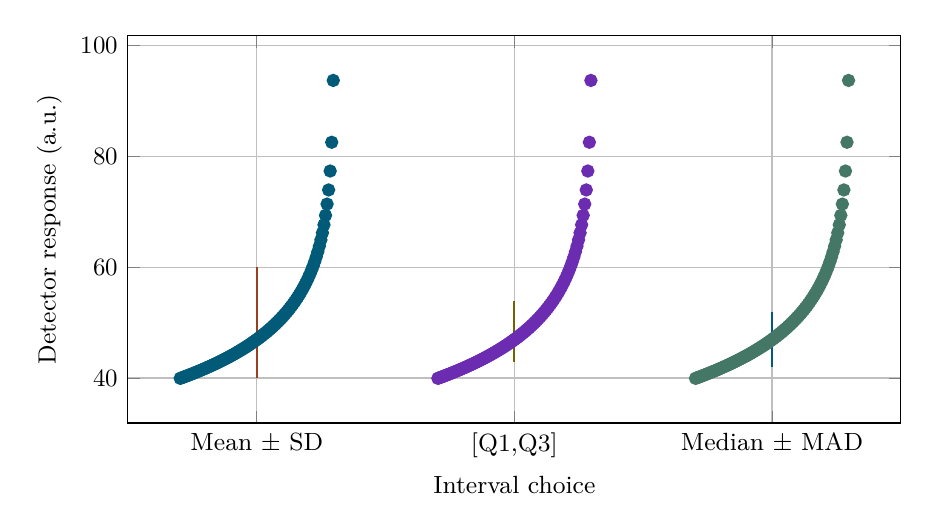
\begin{tikzpicture}
\begin{axis}[width=0.94\linewidth,
height=6.5cm,
scale only axis=false,
grid=major,
tick label style={font=\small},
label style={font=\small},
xlabel={Interval choice},
ylabel={Detector response (a.u.)},
legend style={font=\footnotesize,draw=none,at={(0.5,-0.28)},anchor=north,legend columns=1,text width=0.85\linewidth,align=left},
unbounded coords=jump,
scaled ticks=false,
ymin=31.86651698466225,
ymax=101.75190408505475,
xmin=0.5,
xmax=3.5,
xtick={1,2,3},
xticklabels={{Mean ± SD},{[Q1,Q3]},{Median ± MAD}}]
\addplot[color=pcd1,thick,only marks,mark=*] coordinates {(0.7030000000000001,39.930215496246) (0.7090000000000001,40.032800674276) (0.715,40.136432657911) (0.721,40.24113303134) (0.727,40.346924053282) (0.733,40.453828685386) (0.739,40.56187062215) (0.745,40.671074322438) (0.751,40.781465042716) (0.757,40.893068872116) (0.763,41.00591276944) (0.769,41.120024602253) (0.775,41.235433188192) (0.781,41.352168338646) (0.787,41.470260904983) (0.7929999999999999,41.589742827495) (0.7989999999999999,41.710647187247) (0.8049999999999999,41.833008261065) (0.8109999999999999,41.956861579865) (0.817,42.082243990591) (0.823,42.209193722015) (0.829,42.337750454712) (0.835,42.467955395514) (0.841,42.599851356805) (0.847,42.733482841024) (0.853,42.868896130814) (0.859,43.00613938525) (0.865,43.145262742673) (0.871,43.286318430648) (0.877,43.429360883685) (0.883,43.574446869357) (0.889,43.721635623558) (0.895,43.870988995719) (0.901,44.022571604848) (0.907,44.176451007399) (0.913,44.332697878059) (0.919,44.491386204653) (0.925,44.652593498525) (0.931,44.816401021887) (0.937,44.982894033802) (0.943,45.152162056669) (0.949,45.324299165303) (0.955,45.499404300925) (0.961,45.677581612709) (0.967,45.85894082983) (0.973,46.043597667329) (0.979,46.23167426958) (0.985,46.423299695584) (0.991,46.618610450948) (0.997,46.817751072022) (1.003,47.020874768457) (1.009,47.228144131353) (1.015,47.439731915181) (1.021,47.655821902906) (1.027,47.876609865167) (1.033,48.102304626062) (1.039,48.333129250065) (1.045,48.569322367003) (1.051,48.811139654802) (1.057,49.058855503111) (1.063,49.31276488494) (1.069,49.573185468321) (1.075,49.840460005917) (1.081,50.114959047658) (1.087,50.397084030267) (1.093,50.687270808317) (1.099,50.98599370477) (1.105,51.293770175501) (1.111,51.611166202976) (1.117,51.938802560306) (1.123,52.277362119843) (1.129,52.627598422573) (1.135,52.990345778654) (1.141,53.366531239605) (1.147,53.757188874395) (1.153,54.16347690284) (1.159,54.586698401275) (1.165,55.028326513309) (1.171,55.490035395649) (1.177,55.973738539477) (1.183,56.481636682893) (1.189,57.016278347419) (1.195,57.580637213174) (1.201,58.178212286046) (1.207,58.813159420496) (1.213,59.490466767655) (1.219,60.216193020701) (1.225,60.997797523507) (1.231,61.844608325906) (1.237,62.768503720566) (1.2429999999999999,63.784935940163) (1.249,64.914526391984) (1.255,66.185664030899) (1.2610000000000001,67.638974200483) (1.267,69.335549803636) (1.2730000000000001,71.373530538291) (1.279,73.925841238155) (1.2850000000000001,77.343001548489) (1.291,82.530868055881) (1.297,93.688205573471)};
\addplot[color=pcd2,thick,only marks,mark=*] coordinates {(1.703,39.930215496246) (1.709,40.032800674276) (1.7149999999999999,40.136432657911) (1.721,40.24113303134) (1.7269999999999999,40.346924053282) (1.733,40.453828685386) (1.7389999999999999,40.56187062215) (1.745,40.671074322438) (1.751,40.781465042716) (1.7570000000000001,40.893068872116) (1.763,41.00591276944) (1.769,41.120024602253) (1.775,41.235433188192) (1.781,41.352168338646) (1.787,41.470260904983) (1.793,41.589742827495) (1.799,41.710647187247) (1.805,41.833008261065) (1.811,41.956861579865) (1.817,42.082243990591) (1.823,42.209193722015) (1.829,42.337750454712) (1.835,42.467955395514) (1.841,42.599851356805) (1.847,42.733482841024) (1.853,42.868896130814) (1.859,43.00613938525) (1.865,43.145262742673) (1.871,43.286318430648) (1.877,43.429360883685) (1.883,43.574446869357) (1.889,43.721635623558) (1.895,43.870988995719) (1.901,44.022571604848) (1.907,44.176451007399) (1.913,44.332697878059) (1.919,44.491386204653) (1.925,44.652593498525) (1.931,44.816401021887) (1.937,44.982894033802) (1.943,45.152162056669) (1.949,45.324299165303) (1.955,45.499404300925) (1.961,45.677581612709) (1.967,45.85894082983) (1.973,46.043597667329) (1.979,46.23167426958) (1.985,46.423299695584) (1.991,46.618610450948) (1.997,46.817751072022) (2.003,47.020874768457) (2.009,47.228144131353) (2.015,47.439731915181) (2.021,47.655821902906) (2.027,47.876609865167) (2.033,48.102304626062) (2.039,48.333129250065) (2.045,48.569322367003) (2.051,48.811139654802) (2.057,49.058855503111) (2.063,49.31276488494) (2.069,49.573185468321) (2.075,49.840460005917) (2.081,50.114959047658) (2.087,50.397084030267) (2.093,50.687270808317) (2.099,50.98599370477) (2.105,51.293770175501) (2.111,51.611166202976) (2.117,51.938802560306) (2.123,52.277362119843) (2.129,52.627598422573) (2.135,52.990345778654) (2.141,53.366531239605) (2.147,53.757188874395) (2.153,54.16347690284) (2.159,54.586698401275) (2.165,55.028326513309) (2.171,55.490035395649) (2.177,55.973738539477) (2.183,56.481636682893) (2.189,57.016278347419) (2.195,57.580637213174) (2.201,58.178212286046) (2.207,58.813159420496) (2.213,59.490466767655) (2.219,60.216193020701) (2.225,60.997797523507) (2.231,61.844608325906) (2.237,62.768503720566) (2.243,63.784935940163) (2.249,64.914526391984) (2.255,66.185664030899) (2.261,67.638974200483) (2.267,69.335549803636) (2.273,71.373530538291) (2.279,73.925841238155) (2.285,77.343001548489) (2.291,82.530868055881) (2.297,93.688205573471)};
\addplot[color=pcd3,thick,only marks,mark=*] coordinates {(2.703,39.930215496246) (2.709,40.032800674276) (2.715,40.136432657911) (2.721,40.24113303134) (2.727,40.346924053282) (2.733,40.453828685386) (2.739,40.56187062215) (2.745,40.671074322438) (2.751,40.781465042716) (2.757,40.893068872116) (2.763,41.00591276944) (2.769,41.120024602253) (2.775,41.235433188192) (2.781,41.352168338646) (2.787,41.470260904983) (2.793,41.589742827495) (2.799,41.710647187247) (2.805,41.833008261065) (2.811,41.956861579865) (2.817,42.082243990591) (2.823,42.209193722015) (2.829,42.337750454712) (2.835,42.467955395514) (2.841,42.599851356805) (2.847,42.733482841024) (2.853,42.868896130814) (2.859,43.00613938525) (2.865,43.145262742673) (2.871,43.286318430648) (2.877,43.429360883685) (2.883,43.574446869357) (2.889,43.721635623558) (2.895,43.870988995719) (2.901,44.022571604848) (2.907,44.176451007399) (2.913,44.332697878059) (2.919,44.491386204653) (2.925,44.652593498525) (2.931,44.816401021887) (2.937,44.982894033802) (2.943,45.152162056669) (2.949,45.324299165303) (2.955,45.499404300925) (2.961,45.677581612709) (2.967,45.85894082983) (2.973,46.043597667329) (2.979,46.23167426958) (2.985,46.423299695584) (2.991,46.618610450948) (2.997,46.817751072022) (3.003,47.020874768457) (3.009,47.228144131353) (3.015,47.439731915181) (3.021,47.655821902906) (3.027,47.876609865167) (3.033,48.102304626062) (3.039,48.333129250065) (3.045,48.569322367003) (3.051,48.811139654802) (3.057,49.058855503111) (3.063,49.31276488494) (3.069,49.573185468321) (3.075,49.840460005917) (3.081,50.114959047658) (3.087,50.397084030267) (3.093,50.687270808317) (3.099,50.98599370477) (3.105,51.293770175501) (3.111,51.611166202976) (3.117,51.938802560306) (3.123,52.277362119843) (3.129,52.627598422573) (3.135,52.990345778654) (3.141,53.366531239605) (3.147,53.757188874395) (3.153,54.16347690284) (3.159,54.586698401275) (3.165,55.028326513309) (3.171,55.490035395649) (3.177,55.973738539477) (3.183,56.481636682893) (3.189,57.016278347419) (3.195,57.580637213174) (3.201,58.178212286046) (3.207,58.813159420496) (3.213,59.490466767655) (3.219,60.216193020701) (3.225,60.997797523507) (3.231,61.844608325906) (3.237,62.768503720566) (3.243,63.784935940163) (3.249,64.914526391984) (3.255,66.185664030899) (3.261,67.638974200483) (3.267,69.335549803636) (3.273,71.373530538291) (3.279,73.925841238155) (3.285,77.343001548489) (3.291,82.530868055881) (3.297,93.688205573471)};
\addplot[color=pcd4,thick,mark=none] coordinates {(1,40) (1,60)};
\addplot[color=pcd5,thick,mark=none] coordinates {(2,42.8350428083665) (2,53.85876088150624)};
\addplot[color=pcd1,thick,mark=none] coordinates {(3,42.019552785228) (3,51.819073055251)};

\end{axis}
\end{tikzpicture}
\end{center}


\medskip

\clearpage
\section{A boxplot compresses ordered structure into a comparison view}
A boxplot places the median and quartiles on the measurement axis. Its box therefore provides a compact view of location and central spread. The construction in \hyperref[material-818a681794b0449a267f81516765a4e40e1bc148135f65216ce6e5e91a439a0a]{Fig.~\ref*{material-818a681794b0449a267f81516765a4e40e1bc148135f65216ce6e5e91a439a0a}} connects the ordered observations with those graphical elements. Whiskers and individually displayed extreme points follow the authored convention, which belongs with the plot's interpretation.


\par\medskip
\Needspace{10cm}
\refstepcounter{figure}\label{material-818a681794b0449a267f81516765a4e40e1bc148135f65216ce6e5e91a439a0a}
\noindent\textbf{Fig.~\ref*{material-818a681794b0449a267f81516765a4e40e1bc148135f65216ce6e5e91a439a0a}.} Boxplot construction from the authored ordered observations, quartiles and whisker convention.\par\nopagebreak
\begin{center}
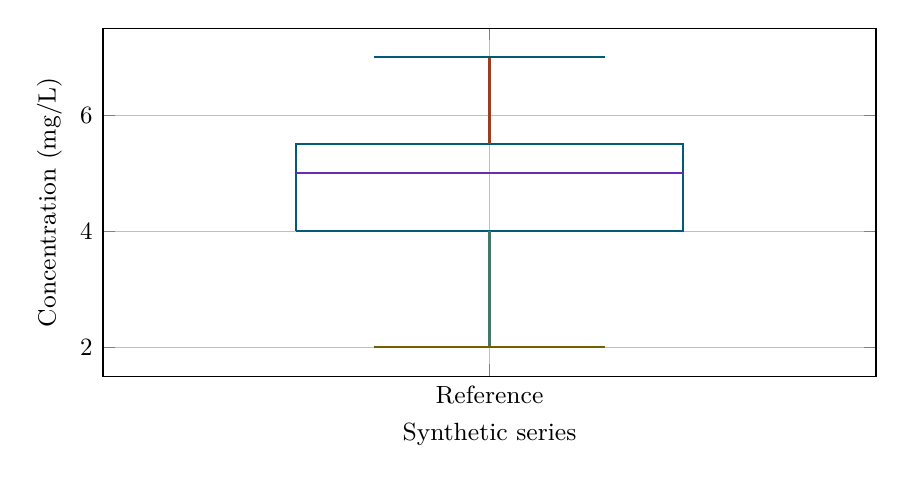
\begin{tikzpicture}
\begin{axis}[width=0.94\linewidth,
height=6cm,
scale only axis=false,
grid=major,
tick label style={font=\small},
label style={font=\small},
xlabel={Synthetic series},
ylabel={Concentration (mg/L)},
legend style={font=\footnotesize,draw=none,at={(0.5,-0.28)},anchor=north,legend columns=1,text width=0.85\linewidth,align=left},
unbounded coords=jump,
scaled ticks=false,
xmin=0.5,
xmax=1.5,
xtick={1},
xticklabels={{Reference}}]
\addplot[color=pcd1,thick,mark=none] coordinates {(0.75,4) (1.25,4) (1.25,5.5) (0.75,5.5) (0.75,4)};
\addplot[color=pcd2,thick,mark=none] coordinates {(0.75,5) (1.25,5)};
\addplot[color=pcd3,thick,mark=none] coordinates {(1,2) (1,4)};
\addplot[color=pcd4,thick,mark=none] coordinates {(1,5.5) (1,7)};
\addplot[color=pcd5,thick,mark=none] coordinates {(0.85,2) (1.15,2)};
\addplot[color=pcd1,thick,mark=none] coordinates {(0.85,7) (1.15,7)};

\end{axis}
\end{tikzpicture}
\end{center}

\medskip

The grouped comparison in \hyperref[material-c5aae8f731d22a332dc51e8890c54fec9780e92b70e85497c610baa5a0f69c86]{Fig.~\ref*{material-c5aae8f731d22a332dc51e8890c54fec9780e92b70e85497c610baa5a0f69c86}} uses this compression to compare several data sets on a common scale. The extreme-value view in \hyperref[material-e3608e54bd8098e425d9379c60bc529214a511389d9f020284383ab26380c01c]{Fig.~\ref*{material-e3608e54bd8098e425d9379c60bc529214a511389d9f020284383ab26380c01c}} keeps unusual observations visible. A flagged observation invites investigation of its measurement and sampling context; the flag is an operational feature of the plotting convention.


\par\medskip
\Needspace{10cm}
\refstepcounter{figure}\label{material-c5aae8f731d22a332dc51e8890c54fec9780e92b70e85497c610baa5a0f69c86}
\noindent\textbf{Fig.~\ref*{material-c5aae8f731d22a332dc51e8890c54fec9780e92b70e85497c610baa5a0f69c86}.} Authored grouped boxplot application on a common measurement scale.\par\nopagebreak
\begin{center}
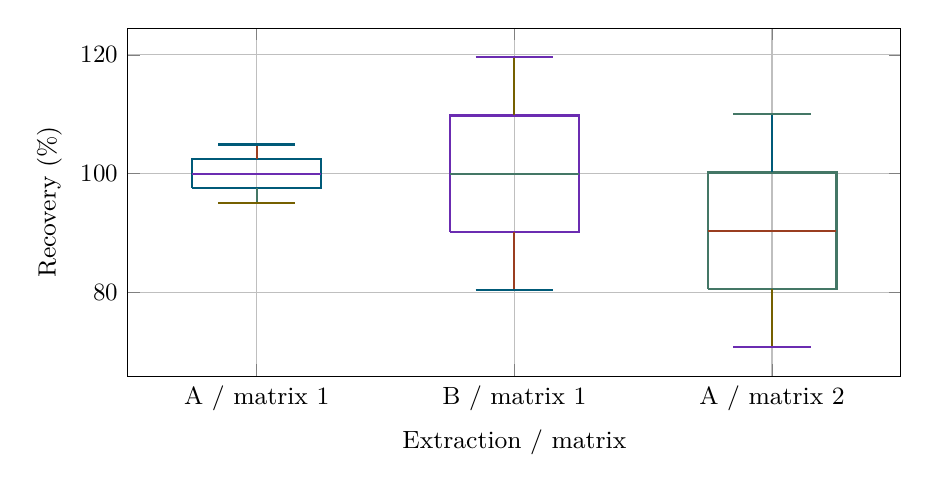
\begin{tikzpicture}
\begin{axis}[width=0.94\linewidth,
height=6cm,
scale only axis=false,
grid=major,
tick label style={font=\small},
label style={font=\small},
xlabel={Extraction / matrix},
ylabel={Recovery (\%)},
legend style={font=\footnotesize,draw=none,at={(0.5,-0.28)},anchor=north,legend columns=1,text width=0.85\linewidth,align=left},
unbounded coords=jump,
scaled ticks=false,
xmin=0.5,
xmax=3.5,
xtick={1,2,3},
xticklabels={{A / matrix 1},{B / matrix 1},{A / matrix 2}}]
\addplot[color=pcd1,thick,mark=none] coordinates {(0.75,97.55) (1.25,97.55) (1.25,102.45) (0.75,102.45) (0.75,97.55)};
\addplot[color=pcd2,thick,mark=none] coordinates {(0.75,100) (1.25,100)};
\addplot[color=pcd3,thick,mark=none] coordinates {(1,95.1) (1,97.55)};
\addplot[color=pcd4,thick,mark=none] coordinates {(1,102.45) (1,104.9)};
\addplot[color=pcd5,thick,mark=none] coordinates {(0.85,95.1) (1.15,95.1)};
\addplot[color=pcd1,thick,mark=none] coordinates {(0.85,104.9) (1.15,104.9)};
\addplot[color=pcd2,thick,mark=none] coordinates {(1.75,90.2) (2.25,90.2) (2.25,109.8) (1.75,109.8) (1.75,90.2)};
\addplot[color=pcd3,thick,mark=none] coordinates {(1.75,100) (2.25,100)};
\addplot[color=pcd4,thick,mark=none] coordinates {(2,80.4) (2,90.2)};
\addplot[color=pcd5,thick,mark=none] coordinates {(2,109.8) (2,119.6)};
\addplot[color=pcd1,thick,mark=none] coordinates {(1.85,80.4) (2.15,80.4)};
\addplot[color=pcd2,thick,mark=none] coordinates {(1.85,119.6) (2.15,119.6)};
\addplot[color=pcd3,thick,mark=none] coordinates {(2.75,80.60000000000001) (3.25,80.60000000000001) (3.25,100.20000000000002) (2.75,100.20000000000002) (2.75,80.60000000000001)};
\addplot[color=pcd4,thick,mark=none] coordinates {(2.75,90.4) (3.25,90.4)};
\addplot[color=pcd5,thick,mark=none] coordinates {(3,70.8) (3,80.60000000000001)};
\addplot[color=pcd1,thick,mark=none] coordinates {(3,100.20000000000002) (3,110)};
\addplot[color=pcd2,thick,mark=none] coordinates {(2.85,70.8) (3.15,70.8)};
\addplot[color=pcd3,thick,mark=none] coordinates {(2.85,110) (3.15,110)};

\end{axis}
\end{tikzpicture}
\end{center}

\medskip

\par\medskip
\Needspace{10cm}
\refstepcounter{figure}\label{material-e3608e54bd8098e425d9379c60bc529214a511389d9f020284383ab26380c01c}
\noindent\textbf{Fig.~\ref*{material-e3608e54bd8098e425d9379c60bc529214a511389d9f020284383ab26380c01c}.} Extreme observations displayed according to the authored boxplot convention.\par\nopagebreak
\begin{center}
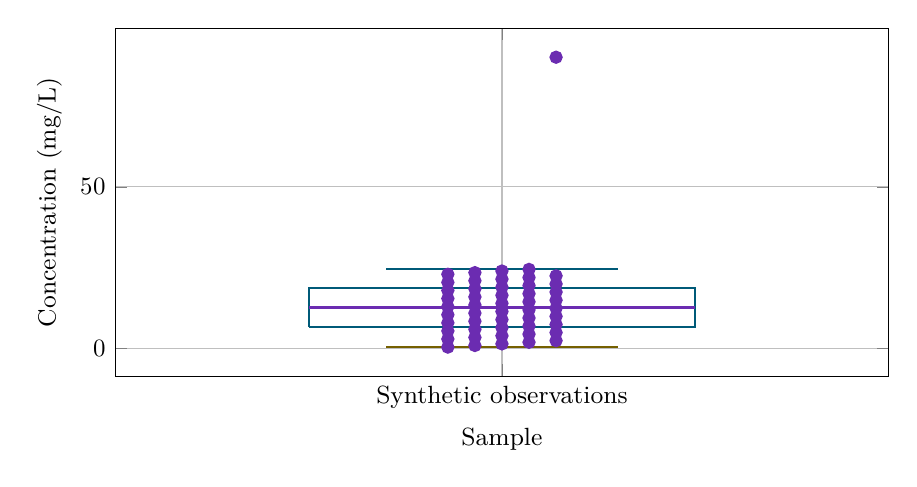
\begin{tikzpicture}
\begin{axis}[width=0.94\linewidth,
height=6cm,
scale only axis=false,
grid=major,
tick label style={font=\small},
label style={font=\small},
xlabel={Sample},
ylabel={Concentration (mg/L)},
legend style={font=\footnotesize,draw=none,at={(0.5,-0.28)},anchor=north,legend columns=1,text width=0.85\linewidth,align=left},
unbounded coords=jump,
scaled ticks=false,
xmin=0.5,
xmax=1.5,
xtick={1},
xticklabels={{Synthetic observations}}]
\addplot[color=pcd1,thick,mark=none] coordinates {(0.75,6.625) (1.25,6.625) (1.25,18.875) (0.75,18.875) (0.75,6.625)};
\addplot[color=pcd2,thick,mark=none] coordinates {(0.75,12.75) (1.25,12.75)};
\addplot[color=pcd3,thick,mark=none] coordinates {(1,0.5) (1,6.625)};
\addplot[color=pcd4,thick,mark=none] coordinates {(1,18.875) (1,24.5)};
\addplot[color=pcd5,thick,mark=none] coordinates {(0.85,0.5) (1.15,0.5)};
\addplot[color=pcd1,thick,mark=none] coordinates {(0.85,24.5) (1.15,24.5)};
\addplot[color=pcd2,thick,only marks,mark=*] coordinates {(0.9299999999999999,0.5) (0.965,1) (1,1.5) (1.035,2) (1.07,2.5) (0.9299999999999999,3) (0.965,3.5) (1,4) (1.035,4.5) (1.07,5) (0.9299999999999999,5.5) (0.965,6) (1,6.5) (1.035,7) (1.07,7.5) (0.9299999999999999,8) (0.965,8.5) (1,9) (1.035,9.5) (1.07,10) (0.9299999999999999,10.5) (0.965,11) (1,11.5) (1.035,12) (1.07,12.5) (0.9299999999999999,13) (0.965,13.5) (1,14) (1.035,14.5) (1.07,15) (0.9299999999999999,15.5) (0.965,16) (1,16.5) (1.035,17) (1.07,17.5) (0.9299999999999999,18) (0.965,18.5) (1,19) (1.035,19.5) (1.07,20) (0.9299999999999999,20.5) (0.965,21) (1,21.5) (1.035,22) (1.07,22.5) (0.9299999999999999,23) (0.965,23.5) (1,24) (1.035,24.5) (1.07,90)};

\end{axis}
\end{tikzpicture}
\end{center}

\medskip

Compression also motivates a complementary view. The bimodal example in \hyperref[material-734defa632ef0ea0d1197dd6debd6db32a6571b9011a6bd5a3f20a62c2f55075]{Fig.~\ref*{material-734defa632ef0ea0d1197dd6debd6db32a6571b9011a6bd5a3f20a62c2f55075}} retains its underlying observations so that grouping within the box can be examined. Dot plots or histograms can show that internal structure directly. The optional source in \hyperref[material-39fc3505ea6908fa800c7e030e8a38c46cf77cfd1bbf7704faa10401a5c154cf]{Listing~\ref*{material-39fc3505ea6908fa800c7e030e8a38c46cf77cfd1bbf7704faa10401a5c154cf}} allows the same data and plotting convention to be reproduced and compared with fuller distribution views.


\par\medskip
\Needspace{10cm}
\refstepcounter{figure}\label{material-734defa632ef0ea0d1197dd6debd6db32a6571b9011a6bd5a3f20a62c2f55075}
\noindent\textbf{Fig.~\ref*{material-734defa632ef0ea0d1197dd6debd6db32a6571b9011a6bd5a3f20a62c2f55075}.} Boxplot and underlying bimodal observations, retaining the two-group structure for comparison.\par\nopagebreak
\begin{center}
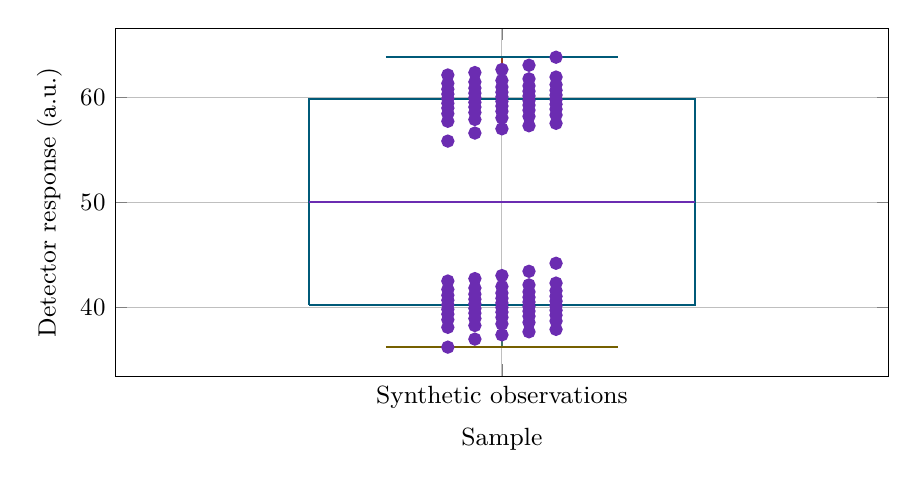
\begin{tikzpicture}
\begin{axis}[width=0.94\linewidth,
height=6cm,
scale only axis=false,
grid=major,
tick label style={font=\small},
label style={font=\small},
xlabel={Sample},
ylabel={Detector response (a.u.)},
legend style={font=\footnotesize,draw=none,at={(0.5,-0.28)},anchor=north,legend columns=1,text width=0.85\linewidth,align=left},
unbounded coords=jump,
scaled ticks=false,
xmin=0.5,
xmax=1.5,
xtick={1},
xticklabels={{Synthetic observations}}]
\addplot[color=pcd1,thick,mark=none] coordinates {(0.75,40.216921725550996) (1.25,40.216921725550996) (1.25,59.783078274449004) (0.75,59.783078274449004) (0.75,40.216921725550996)};
\addplot[color=pcd2,thick,mark=none] coordinates {(0.75,50) (1.25,50)};
\addplot[color=pcd3,thick,mark=none] coordinates {(1,36.203861904595) (1,40.216921725550996)};
\addplot[color=pcd4,thick,mark=none] coordinates {(1,59.783078274449004) (1,63.796138095405)};
\addplot[color=pcd5,thick,mark=none] coordinates {(0.85,36.203861904595) (1.15,36.203861904595)};
\addplot[color=pcd1,thick,mark=none] coordinates {(0.85,63.796138095405) (1.15,63.796138095405)};
\addplot[color=pcd2,thick,only marks,mark=*] coordinates {(0.9299999999999999,36.203861904595) (0.965,36.968344965996) (1,37.373171342811) (1.035,37.663249348955) (1.07,37.894944427129) (0.9299999999999999,38.090935235275) (0.965,38.26275052086) (1,38.417100222768) (1.035,38.558256085355) (1.07,38.689118543731) (0.9299999999999999,38.811755599904) (0.965,38.927699911254) (1,39.038123973652) (1.035,39.143949102676) (1.07,39.245916271163) (0.9299999999999999,39.344633882841) (0.965,39.44061103123) (1,39.534281313527) (1.035,39.626020324213) (1.07,39.716158820762) (0.9299999999999999,39.804992871389) (0.965,39.892791871197) (1,39.979805043931) (1.035,40.066266872452) (1.07,40.152401787581) (0.9299999999999999,40.238428371541) (0.965,40.324563286669) (1,40.411025115191) (1.035,40.498038287925) (1.07,40.585837287733) (0.9299999999999999,40.674671338359) (0.965,40.764809834908) (1,40.856548845594) (1.035,40.950219127892) (1.07,41.04619627628) (0.9299999999999999,41.144913887958) (0.965,41.246881056446) (1,41.352706185469) (1.035,41.463130247867) (1.07,41.579074559217) (0.9299999999999999,41.70171161539) (0.965,41.832574073766) (1,41.973729936353) (1.035,42.128079638261) (1.07,42.299894923847) (0.9299999999999999,42.495885731992) (0.965,42.727580810167) (1,43.01765881631) (1.035,43.422485193125) (1.07,44.186968254526) (0.9299999999999999,55.813031745474) (0.965,56.577514806875) (1,56.98234118369) (1.035,57.272419189833) (1.07,57.504114268008) (0.9299999999999999,57.700105076153) (0.965,57.871920361739) (1,58.026270063647) (1.035,58.167425926234) (1.07,58.29828838461) (0.9299999999999999,58.420925440783) (0.965,58.536869752133) (1,58.647293814531) (1.035,58.753118943554) (1.07,58.855086112042) (0.9299999999999999,58.95380372372) (0.965,59.049780872108) (1,59.143451154406) (1.035,59.235190165092) (1.07,59.325328661641) (0.9299999999999999,59.414162712267) (0.965,59.501961712075) (1,59.588974884809) (1.035,59.675436713331) (1.07,59.761571628459) (0.9299999999999999,59.847598212419) (0.965,59.933733127548) (1,60.020194956069) (1.035,60.107208128803) (1.07,60.195007128611) (0.9299999999999999,60.283841179238) (0.965,60.373979675787) (1,60.465718686473) (1.035,60.55938896877) (1.07,60.655366117159) (0.9299999999999999,60.754083728837) (0.965,60.856050897324) (1,60.961876026348) (1.035,61.072300088746) (1.07,61.188244400096) (0.9299999999999999,61.310881456269) (0.965,61.441743914645) (1,61.582899777232) (1.035,61.73724947914) (1.07,61.909064764725) (0.9299999999999999,62.105055572871) (0.965,62.336750651045) (1,62.626828657189) (1.035,63.031655034004) (1.07,63.796138095405)};

\end{axis}
\end{tikzpicture}
\end{center}

\medskip

\par\medskip
\Needspace{8\baselineskip}
\refstepcounter{listing}\label{material-39fc3505ea6908fa800c7e030e8a38c46cf77cfd1bbf7704faa10401a5c154cf}
\noindent\textbf{Listing~\ref*{material-39fc3505ea6908fa800c7e030e8a38c46cf77cfd1bbf7704faa10401a5c154cf}.} Optional R source for reproducing the boxplot data and comparison views.\par\nopagebreak
\begin{Verbatim}[fontsize=\footnotesize,breaklines=true,breakanywhere=true]
if (!requireNamespace("ggplot2", quietly = TRUE)) {
  if (requireNamespace("webr", quietly = TRUE)) webr::install("ggplot2")
  else stop("Install ggplot2 first: install.packages('ggplot2')")
}
library(ggplot2)
groups <- c("A / matrix 1", "B / matrix 1", "A / matrix 2")
d <- data.frame(series = rep(groups, each = 50),
  value = c(seq(95.1, by=0.2, length.out=50),
            seq(80.4, by=0.8, length.out=50),
            seq(70.8, by=0.8, length.out=50)))
d$value[150] <- 110
d$series <- factor(d$series, levels = groups)
p <- ggplot(d, aes(series, value)) +
  geom_boxplot(coef = 1.5) +
  labs(x = "Synthetic extraction / matrix", y = "Recovery (%)") +
  theme_minimal(base_size = 16)
print(p)
ggplot_build(p)$data[[1]][c("lower", "middle", "upper", "ymin", "ymax", "outliers")]
\end{Verbatim}

\par\noindent\textbf{ggplot() + aes()}

Map the extraction/matrix group to x and recovery (\%) to y.

\par\noindent\textbf{geom\_boxplot(coef=1.5)}

Use ggplot2's usual linearly interpolated quartiles and 1.5\ensuremath{\times}IQR fences; flag rather than remove distant values.

\par\noindent\textbf{ggplot\_build(p)\$data[[1]]}

Inspect the computed quartiles, whisker endpoints and separately plotted observations.

\par\noindent\textbf{c(...)}

\textbf{Combine} values or output-column names into a vector; does not sort them.

\par\noindent\textbf{data.frame(...)}

Build a table with one row per synthetic observation and named series/value columns.

\par\noindent\textbf{seq(...)}

Generate a synthetic grid: \textbf{by} sets its increment; \textbf{length.out} sets the number of values.

\par\noindent\textbf{rep(groups, each=50)}

Repeat every group label \textbf{50 times}, aligning labels with the synthetic observations.

\par\noindent\textbf{factor(..., levels=groups)}

Declare categories and their display order; the recovery values do not change.

\par\noindent\textbf{requireNamespace(..., quietly=TRUE)}

Check package availability without attaching it. TRUE/FALSE selects the setup branch.

\par\noindent\textbf{webr::install("ggplot2")}

Download ggplot2 into browser R if missing. \textbf{Network required}; learner observations are not uploaded.

\par\noindent\textbf{stop(...)}

Stop with a setup error. Desktop R needs ggplot2 installed separately.

\par\noindent\textbf{library(ggplot2)}

Attach the installed package so its functions can be called by name.

\par\noindent\textbf{print(p)}

Draw the ggplot object explicitly in the browser R runtime.

\par\noindent\textbf{labs(x=..., y=...)}

Label axes, including the \textbf{recovery unit (\%)}.

\par\noindent\textbf{theme\_minimal(base\_size=16)}

Set the plot theme and base font size; \textbf{appearance only}, not a statistical calculation.

\par\noindent\textbf{<-, \$, [, [[, +, if / else, ! and ::}

\textbf{<-} assigns; \textbf{\$} selects a column; \textbf{[} subsets; \textbf{[[} extracts a list element. \textbf{+} adds ggplot layers; \textbf{if/else} branches; \textbf{!} negates; \textbf{::} selects a package function.

\medskip

\clearpage
\section{Histogram bins determine the resolution of the observed shape}
A histogram groups numerical observations into intervals. The authored Normal, skewed and bimodal examples (\hyperref[material-7e65fe053d8b42321b97e524362bc0df0551ef2630fbb9af0419dbd570af6100]{Fig.~\ref*{material-7e65fe053d8b42321b97e524362bc0df0551ef2630fbb9af0419dbd570af6100}}, \hyperref[material-989fdc1f61d3d5cea1d8316d8e82fb47999615869cc1aadec9e9fcd4fc2d959e]{Fig.~\ref*{material-989fdc1f61d3d5cea1d8316d8e82fb47999615869cc1aadec9e9fcd4fc2d959e}}, \hyperref[material-0e1006c588730dbed14461bad18d5e12458d703e25b4c01316e323961041b0fc]{Fig.~\ref*{material-0e1006c588730dbed14461bad18d5e12458d703e25b4c01316e323961041b0fc}}) show how the resulting bars describe concentration, asymmetry and grouping. Each view is an empirical summary at a selected resolution.


\par\medskip
\Needspace{10cm}
\refstepcounter{figure}\label{material-7e65fe053d8b42321b97e524362bc0df0551ef2630fbb9af0419dbd570af6100}
\noindent\textbf{Fig.~\ref*{material-7e65fe053d8b42321b97e524362bc0df0551ef2630fbb9af0419dbd570af6100}.} Histogram of the authored Normal example with its fixed bins and axis normalization.\par\nopagebreak
\begin{center}
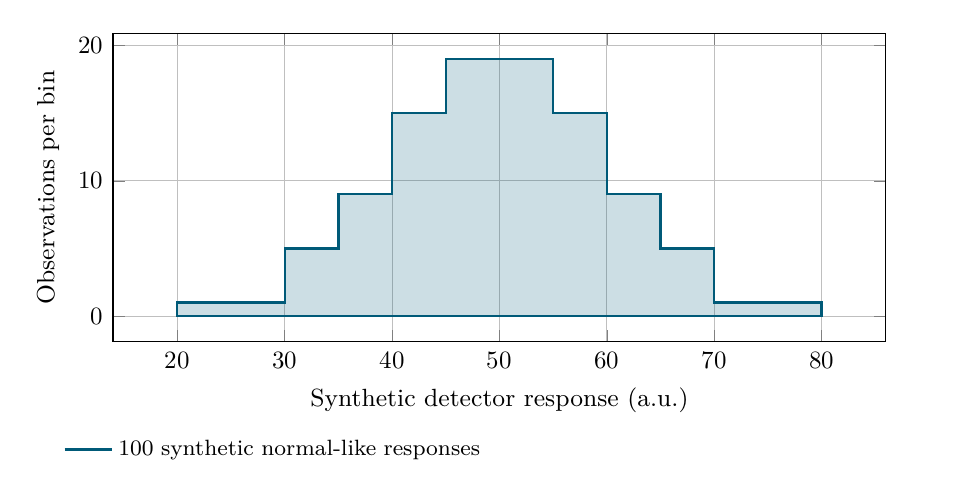
\begin{tikzpicture}
\begin{axis}[width=0.94\linewidth,
height=5.5cm,
scale only axis=false,
grid=major,
tick label style={font=\small},
label style={font=\small},
xlabel={Synthetic detector response (a.u.)},
ylabel={Observations per bin},
legend style={font=\footnotesize,draw=none,at={(0.5,-0.28)},anchor=north,legend columns=1,text width=0.85\linewidth,align=left},
unbounded coords=jump,
scaled ticks=false]
\addplot[color=pcd1,thick,mark=none,fill=pcd1,fill opacity=0.2] coordinates {(20,0) (20,1) (25,1) (25,1) (30,1) (30,5) (35,5) (35,9) (40,9) (40,15) (45,15) (45,19) (50,19) (50,19) (55,19) (55,15) (60,15) (60,9) (65,9) (65,5) (70,5) (70,1) (75,1) (75,1) (80,1) (80,0)} \closedcycle;
\addlegendentry{100 synthetic normal-like responses}

\end{axis}
\end{tikzpicture}
\end{center}

\medskip

\par\medskip
\Needspace{10cm}
\refstepcounter{figure}\label{material-989fdc1f61d3d5cea1d8316d8e82fb47999615869cc1aadec9e9fcd4fc2d959e}
\noindent\textbf{Fig.~\ref*{material-989fdc1f61d3d5cea1d8316d8e82fb47999615869cc1aadec9e9fcd4fc2d959e}.} Histogram of the authored right-skewed observations.\par\nopagebreak
\begin{center}
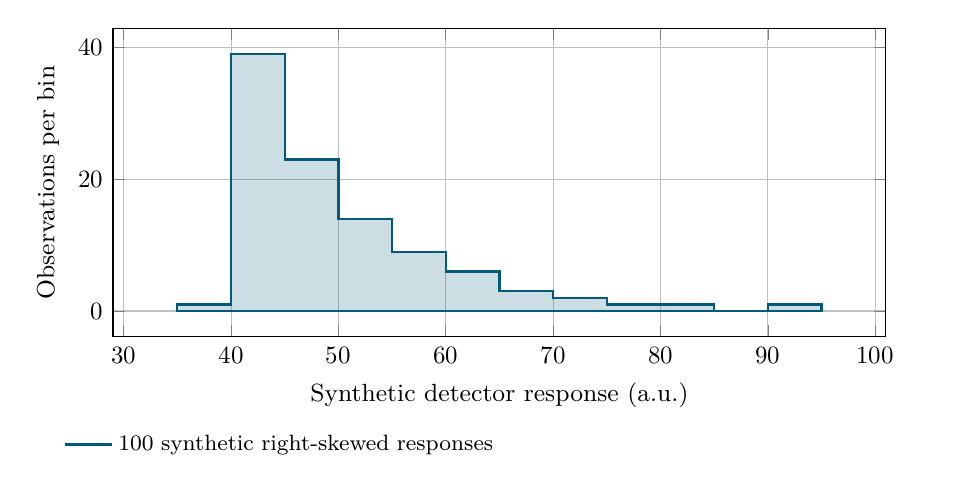
\begin{tikzpicture}
\begin{axis}[width=0.94\linewidth,
height=5.5cm,
scale only axis=false,
grid=major,
tick label style={font=\small},
label style={font=\small},
xlabel={Synthetic detector response (a.u.)},
ylabel={Observations per bin},
legend style={font=\footnotesize,draw=none,at={(0.5,-0.28)},anchor=north,legend columns=1,text width=0.85\linewidth,align=left},
unbounded coords=jump,
scaled ticks=false]
\addplot[color=pcd1,thick,mark=none,fill=pcd1,fill opacity=0.2] coordinates {(35,0) (35,1) (40,1) (40,39) (45,39) (45,23) (50,23) (50,14) (55,14) (55,9) (60,9) (60,6) (65,6) (65,3) (70,3) (70,2) (75,2) (75,1) (80,1) (80,1) (85,1) (85,0) (90,0) (90,1) (95,1) (95,0)} \closedcycle;
\addlegendentry{100 synthetic right-skewed responses}

\end{axis}
\end{tikzpicture}
\end{center}

\medskip

\par\medskip
\Needspace{10cm}
\refstepcounter{figure}\label{material-0e1006c588730dbed14461bad18d5e12458d703e25b4c01316e323961041b0fc}
\noindent\textbf{Fig.~\ref*{material-0e1006c588730dbed14461bad18d5e12458d703e25b4c01316e323961041b0fc}.} Histogram of the authored bimodal observations at the selected reference binning.\par\nopagebreak
\begin{center}
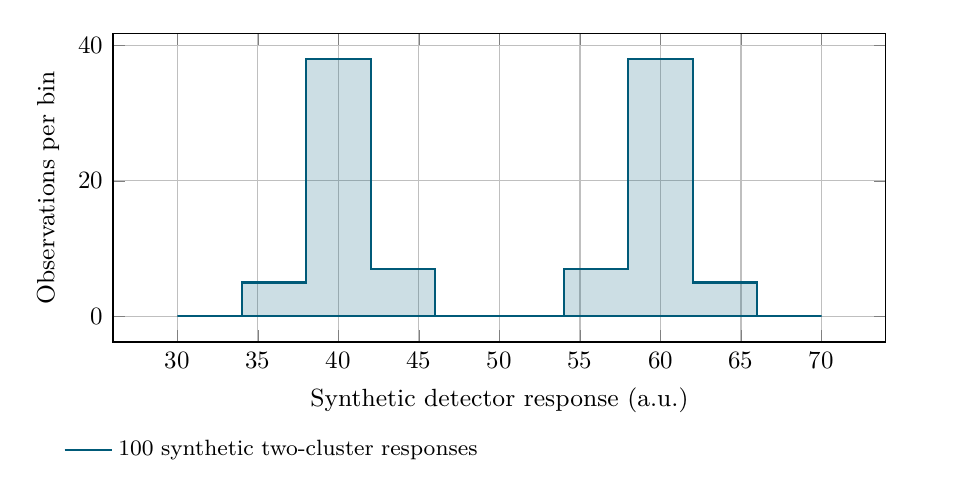
\begin{tikzpicture}
\begin{axis}[width=0.94\linewidth,
height=5.5cm,
scale only axis=false,
grid=major,
tick label style={font=\small},
label style={font=\small},
xlabel={Synthetic detector response (a.u.)},
ylabel={Observations per bin},
legend style={font=\footnotesize,draw=none,at={(0.5,-0.28)},anchor=north,legend columns=1,text width=0.85\linewidth,align=left},
unbounded coords=jump,
scaled ticks=false]
\addplot[color=pcd1,thick,mark=none,fill=pcd1,fill opacity=0.2] coordinates {(30,0) (30,0) (34,0) (34,5) (38,5) (38,38) (42,38) (42,7) (46,7) (46,0) (50,0) (50,0) (54,0) (54,7) (58,7) (58,38) (62,38) (62,5) (66,5) (66,0) (70,0) (70,0)} \closedcycle;
\addlegendentry{100 synthetic two-cluster responses}

\end{axis}
\end{tikzpicture}
\end{center}

\medskip

Bin width changes that resolution. The coarse and fine views in \hyperref[material-40fa88f5af6f61918e0482f62e47d6ea8529ec21c730b3f4de6cfd8387a3011e]{Fig.~\ref*{material-40fa88f5af6f61918e0482f62e47d6ea8529ec21c730b3f4de6cfd8387a3011e}} and \hyperref[material-48a891902bf6de9e0629efb13f74fe69935dfc9d98d84e11e05a327bfc5742ff]{Fig.~\ref*{material-48a891902bf6de9e0629efb13f74fe69935dfc9d98d84e11e05a327bfc5742ff}} trade broad smoothing against sensitivity to small-scale sampling variation. The origin comparison in \hyperref[material-9b8219b4da5a6a0164a2986eab5296214a3f7eba1a0b3aeff12e9032010d8086]{Fig.~\ref*{material-9b8219b4da5a6a0164a2986eab5296214a3f7eba1a0b3aeff12e9032010d8086}} adds a second choice: moving the interval boundaries changes which nearby observations share a bin. Comparing several reasonable settings helps distinguish stable structure from the particular partition.


\par\medskip
\Needspace{10cm}
\refstepcounter{figure}\label{material-40fa88f5af6f61918e0482f62e47d6ea8529ec21c730b3f4de6cfd8387a3011e}
\noindent\textbf{Fig.~\ref*{material-40fa88f5af6f61918e0482f62e47d6ea8529ec21c730b3f4de6cfd8387a3011e}.} Coarse-bin view of the authored comparison data.\par\nopagebreak
\begin{center}
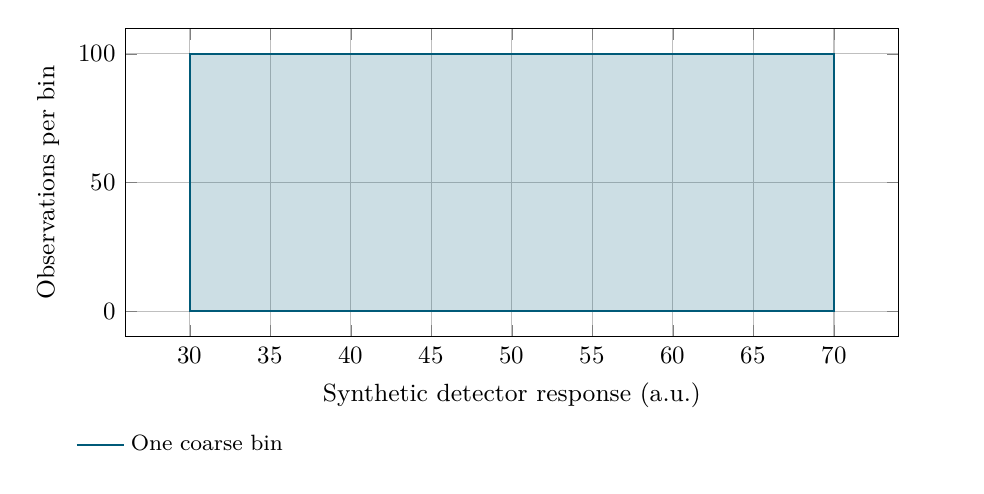
\begin{tikzpicture}
\begin{axis}[width=0.94\linewidth,
height=5.5cm,
scale only axis=false,
grid=major,
tick label style={font=\small},
label style={font=\small},
xlabel={Synthetic detector response (a.u.)},
ylabel={Observations per bin},
legend style={font=\footnotesize,draw=none,at={(0.5,-0.28)},anchor=north,legend columns=1,text width=0.85\linewidth,align=left},
unbounded coords=jump,
scaled ticks=false]
\addplot[color=pcd1,thick,mark=none,fill=pcd1,fill opacity=0.2] coordinates {(30,0) (30,100) (70,100) (70,0)} \closedcycle;
\addlegendentry{One coarse bin}

\end{axis}
\end{tikzpicture}
\end{center}

\medskip

\par\medskip
\Needspace{10cm}
\refstepcounter{figure}\label{material-48a891902bf6de9e0629efb13f74fe69935dfc9d98d84e11e05a327bfc5742ff}
\noindent\textbf{Fig.~\ref*{material-48a891902bf6de9e0629efb13f74fe69935dfc9d98d84e11e05a327bfc5742ff}.} Fine-bin view of the same authored comparison data.\par\nopagebreak
\begin{center}
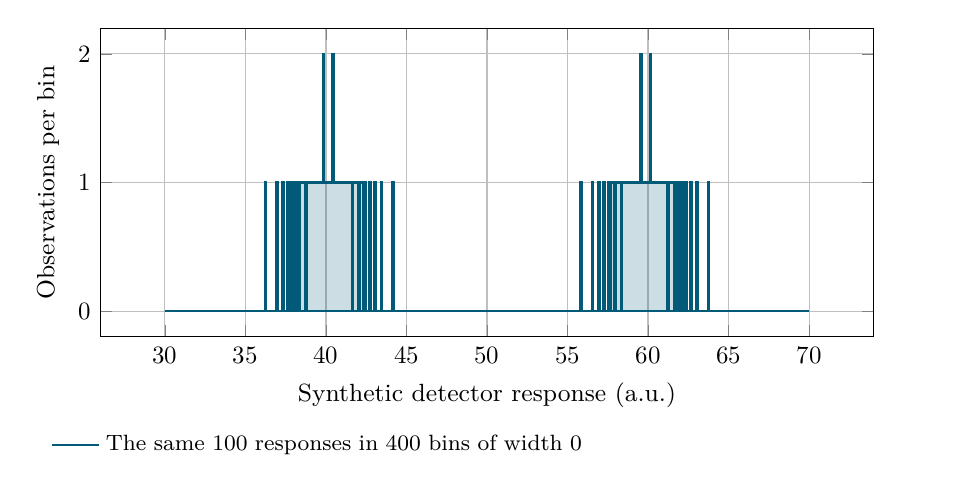
\begin{tikzpicture}
\begin{axis}[width=0.94\linewidth,
height=5.5cm,
scale only axis=false,
grid=major,
tick label style={font=\small},
label style={font=\small},
xlabel={Synthetic detector response (a.u.)},
ylabel={Observations per bin},
legend style={font=\footnotesize,draw=none,at={(0.5,-0.28)},anchor=north,legend columns=1,text width=0.85\linewidth,align=left},
unbounded coords=jump,
scaled ticks=false]
\addplot[color=pcd1,thick,mark=none,fill=pcd1,fill opacity=0.2] coordinates {(30,0) (30,0) (30.1,0) (30.1,0) (30.2,0) (30.2,0) (30.3,0) (30.3,0) (30.4,0) (30.4,0) (30.5,0) (30.5,0) (30.6,0) (30.6,0) (30.7,0) (30.7,0) (30.8,0) (30.8,0) (30.9,0) (30.9,0) (31,0) (31,0) (31.1,0) (31.1,0) (31.2,0) (31.2,0) (31.3,0) (31.3,0) (31.4,0) (31.4,0) (31.5,0) (31.5,0) (31.6,0) (31.6,0) (31.7,0) (31.7,0) (31.8,0) (31.8,0) (31.9,0) (31.9,0) (32,0) (32,0) (32.1,0) (32.1,0) (32.2,0) (32.2,0) (32.3,0) (32.3,0) (32.4,0) (32.4,0) (32.5,0) (32.5,0) (32.6,0) (32.6,0) (32.7,0) (32.7,0) (32.8,0) (32.8,0) (32.9,0) (32.9,0) (33,0) (33,0) (33.1,0) (33.1,0) (33.2,0) (33.2,0) (33.3,0) (33.3,0) (33.4,0) (33.4,0) (33.5,0) (33.5,0) (33.6,0) (33.6,0) (33.7,0) (33.7,0) (33.8,0) (33.8,0) (33.9,0) (33.9,0) (34,0) (34,0) (34.1,0) (34.1,0) (34.2,0) (34.2,0) (34.3,0) (34.3,0) (34.4,0) (34.4,0) (34.5,0) (34.5,0) (34.6,0) (34.6,0) (34.7,0) (34.7,0) (34.8,0) (34.8,0) (34.9,0) (34.9,0) (35,0) (35,0) (35.1,0) (35.1,0) (35.2,0) (35.2,0) (35.3,0) (35.3,0) (35.4,0) (35.4,0) (35.5,0) (35.5,0) (35.6,0) (35.6,0) (35.7,0) (35.7,0) (35.8,0) (35.8,0) (35.9,0) (35.9,0) (36,0) (36,0) (36.1,0) (36.1,0) (36.2,0) (36.2,1) (36.3,1) (36.3,0) (36.4,0) (36.4,0) (36.5,0) (36.5,0) (36.6,0) (36.6,0) (36.7,0) (36.7,0) (36.8,0) (36.8,0) (36.9,0) (36.9,1) (37,1) (37,0) (37.1,0) (37.1,0) (37.2,0) (37.2,0) (37.3,0) (37.3,1) (37.4,1) (37.4,0) (37.5,0) (37.5,0) (37.6,0) (37.6,1) (37.7,1) (37.7,0) (37.8,0) (37.8,1) (37.9,1) (37.9,0) (38,0) (38,1) (38.1,1) (38.1,0) (38.2,0) (38.2,1) (38.3,1) (38.3,0) (38.4,0) (38.4,1) (38.5,1) (38.5,1) (38.6,1) (38.6,1) (38.7,1) (38.7,0) (38.8,0) (38.8,1) (38.9,1) (38.9,1) (39,1) (39,1) (39.1,1) (39.1,1) (39.2,1) (39.2,1) (39.3,1) (39.3,1) (39.4,1) (39.4,1) (39.5,1) (39.5,1) (39.6,1) (39.6,1) (39.7,1) (39.7,1) (39.8,1) (39.8,2) (39.9,2) (39.9,1) (40,1) (40,1) (40.1,1) (40.1,1) (40.2,1) (40.2,1) (40.3,1) (40.3,1) (40.4,1) (40.4,2) (40.5,2) (40.5,1) (40.6,1) (40.6,1) (40.7,1) (40.7,1) (40.8,1) (40.8,1) (40.9,1) (40.9,1) (41,1) (41,1) (41.1,1) (41.1,1) (41.2,1) (41.2,1) (41.3,1) (41.3,1) (41.4,1) (41.4,1) (41.5,1) (41.5,1) (41.6,1) (41.6,0) (41.7,0) (41.7,1) (41.8,1) (41.8,1) (41.9,1) (41.9,1) (42,1) (42,0) (42.1,0) (42.1,1) (42.2,1) (42.2,1) (42.3,1) (42.3,0) (42.4,0) (42.4,1) (42.5,1) (42.5,0) (42.6,0) (42.6,0) (42.7,0) (42.7,1) (42.8,1) (42.8,0) (42.9,0) (42.9,0) (43,0) (43,1) (43.1,1) (43.1,0) (43.2,0) (43.2,0) (43.3,0) (43.3,0) (43.4,0) (43.4,1) (43.5,1) (43.5,0) (43.6,0) (43.6,0) (43.7,0) (43.7,0) (43.8,0) (43.8,0) (43.9,0) (43.9,0) (44,0) (44,0) (44.1,0) (44.1,1) (44.2,1) (44.2,0) (44.3,0) (44.3,0) (44.4,0) (44.4,0) (44.5,0) (44.5,0) (44.6,0) (44.6,0) (44.7,0) (44.7,0) (44.8,0) (44.8,0) (44.9,0) (44.9,0) (45,0) (45,0) (45.1,0) (45.1,0) (45.2,0) (45.2,0) (45.3,0) (45.3,0) (45.4,0) (45.4,0) (45.5,0) (45.5,0) (45.6,0) (45.6,0) (45.7,0) (45.7,0) (45.8,0) (45.8,0) (45.9,0) (45.9,0) (46,0) (46,0) (46.1,0) (46.1,0) (46.2,0) (46.2,0) (46.3,0) (46.3,0) (46.4,0) (46.4,0) (46.5,0) (46.5,0) (46.6,0) (46.6,0) (46.7,0) (46.7,0) (46.8,0) (46.8,0) (46.9,0) (46.9,0) (47,0) (47,0) (47.1,0) (47.1,0) (47.2,0) (47.2,0) (47.3,0) (47.3,0) (47.4,0) (47.4,0) (47.5,0) (47.5,0) (47.6,0) (47.6,0) (47.7,0) (47.7,0) (47.8,0) (47.8,0) (47.9,0) (47.9,0) (48,0) (48,0) (48.1,0) (48.1,0) (48.2,0) (48.2,0) (48.3,0) (48.3,0) (48.4,0) (48.4,0) (48.5,0) (48.5,0) (48.6,0) (48.6,0) (48.7,0) (48.7,0) (48.8,0) (48.8,0) (48.9,0) (48.9,0) (49,0) (49,0) (49.1,0) (49.1,0) (49.2,0) (49.2,0) (49.3,0) (49.3,0) (49.4,0) (49.4,0) (49.5,0) (49.5,0) (49.6,0) (49.6,0) (49.7,0) (49.7,0) (49.8,0) (49.8,0) (49.9,0) (49.9,0) (50,0) (50,0) (50.1,0) (50.1,0) (50.2,0) (50.2,0) (50.3,0) (50.3,0) (50.4,0) (50.4,0) (50.5,0) (50.5,0) (50.6,0) (50.6,0) (50.7,0) (50.7,0) (50.8,0) (50.8,0) (50.9,0) (50.9,0) (51,0) (51,0) (51.1,0) (51.1,0) (51.2,0) (51.2,0) (51.3,0) (51.3,0) (51.4,0) (51.4,0) (51.5,0) (51.5,0) (51.6,0) (51.6,0) (51.7,0) (51.7,0) (51.8,0) (51.8,0) (51.9,0) (51.9,0) (52,0) (52,0) (52.1,0) (52.1,0) (52.2,0) (52.2,0) (52.3,0) (52.3,0) (52.4,0) (52.4,0) (52.5,0) (52.5,0) (52.6,0) (52.6,0) (52.7,0) (52.7,0) (52.8,0) (52.8,0) (52.9,0) (52.9,0) (53,0) (53,0) (53.1,0) (53.1,0) (53.2,0) (53.2,0) (53.3,0) (53.3,0) (53.4,0) (53.4,0) (53.5,0) (53.5,0) (53.6,0) (53.6,0) (53.7,0) (53.7,0) (53.8,0) (53.8,0) (53.9,0) (53.9,0) (54,0) (54,0) (54.1,0) (54.1,0) (54.2,0) (54.2,0) (54.3,0) (54.3,0) (54.4,0) (54.4,0) (54.5,0) (54.5,0) (54.6,0) (54.6,0) (54.7,0) (54.7,0) (54.8,0) (54.8,0) (54.9,0) (54.9,0) (55,0) (55,0) (55.1,0) (55.1,0) (55.2,0) (55.2,0) (55.3,0) (55.3,0) (55.4,0) (55.4,0) (55.5,0) (55.5,0) (55.6,0) (55.6,0) (55.7,0) (55.7,0) (55.8,0) (55.8,1) (55.9,1) (55.9,0) (56,0) (56,0) (56.1,0) (56.1,0) (56.2,0) (56.2,0) (56.3,0) (56.3,0) (56.4,0) (56.4,0) (56.5,0) (56.5,1) (56.6,1) (56.6,0) (56.7,0) (56.7,0) (56.8,0) (56.8,0) (56.9,0) (56.9,1) (57,1) (57,0) (57.1,0) (57.1,0) (57.2,0) (57.2,1) (57.3,1) (57.3,0) (57.4,0) (57.4,0) (57.5,0) (57.5,1) (57.6,1) (57.6,0) (57.7,0) (57.7,1) (57.8,1) (57.8,1) (57.9,1) (57.9,0) (58,0) (58,1) (58.1,1) (58.1,1) (58.2,1) (58.2,1) (58.3,1) (58.3,0) (58.4,0) (58.4,1) (58.5,1) (58.5,1) (58.6,1) (58.6,1) (58.7,1) (58.7,1) (58.8,1) (58.8,1) (58.9,1) (58.9,1) (59,1) (59,1) (59.1,1) (59.1,1) (59.2,1) (59.2,1) (59.3,1) (59.3,1) (59.4,1) (59.4,1) (59.5,1) (59.5,2) (59.6,2) (59.6,1) (59.7,1) (59.7,1) (59.8,1) (59.8,1) (59.9,1) (59.9,1) (60,1) (60,1) (60.1,1) (60.1,2) (60.2,2) (60.2,1) (60.3,1) (60.3,1) (60.4,1) (60.4,1) (60.5,1) (60.5,1) (60.6,1) (60.6,1) (60.7,1) (60.7,1) (60.8,1) (60.8,1) (60.9,1) (60.9,1) (61,1) (61,1) (61.1,1) (61.1,1) (61.2,1) (61.2,0) (61.3,0) (61.3,1) (61.4,1) (61.4,1) (61.5,1) (61.5,1) (61.6,1) (61.6,0) (61.7,0) (61.7,1) (61.8,1) (61.8,0) (61.9,0) (61.9,1) (62,1) (62,0) (62.1,0) (62.1,1) (62.2,1) (62.2,0) (62.3,0) (62.3,1) (62.4,1) (62.4,0) (62.5,0) (62.5,0) (62.6,0) (62.6,1) (62.7,1) (62.7,0) (62.8,0) (62.8,0) (62.9,0) (62.9,0) (63,0) (63,1) (63.1,1) (63.1,0) (63.2,0) (63.2,0) (63.3,0) (63.3,0) (63.4,0) (63.4,0) (63.5,0) (63.5,0) (63.6,0) (63.6,0) (63.7,0) (63.7,1) (63.8,1) (63.8,0) (63.9,0) (63.9,0) (64,0) (64,0) (64.1,0) (64.1,0) (64.2,0) (64.2,0) (64.3,0) (64.3,0) (64.4,0) (64.4,0) (64.5,0) (64.5,0) (64.6,0) (64.6,0) (64.7,0) (64.7,0) (64.8,0) (64.8,0) (64.9,0) (64.9,0) (65,0) (65,0) (65.1,0) (65.1,0) (65.2,0) (65.2,0) (65.3,0) (65.3,0) (65.4,0) (65.4,0) (65.5,0) (65.5,0) (65.6,0) (65.6,0) (65.7,0) (65.7,0) (65.8,0) (65.8,0) (65.9,0) (65.9,0) (66,0) (66,0) (66.1,0) (66.1,0) (66.2,0) (66.2,0) (66.3,0) (66.3,0) (66.4,0) (66.4,0) (66.5,0) (66.5,0) (66.6,0) (66.6,0) (66.7,0) (66.7,0) (66.8,0) (66.8,0) (66.9,0) (66.9,0) (67,0) (67,0) (67.1,0) (67.1,0) (67.2,0) (67.2,0) (67.3,0) (67.3,0) (67.4,0) (67.4,0) (67.5,0) (67.5,0) (67.6,0) (67.6,0) (67.7,0) (67.7,0) (67.8,0) (67.8,0) (67.9,0) (67.9,0) (68,0) (68,0) (68.1,0) (68.1,0) (68.2,0) (68.2,0) (68.3,0) (68.3,0) (68.4,0) (68.4,0) (68.5,0) (68.5,0) (68.6,0) (68.6,0) (68.7,0) (68.7,0) (68.8,0) (68.8,0) (68.9,0) (68.9,0) (69,0) (69,0) (69.1,0) (69.1,0) (69.2,0) (69.2,0) (69.3,0) (69.3,0) (69.4,0) (69.4,0) (69.5,0) (69.5,0) (69.6,0) (69.6,0) (69.7,0) (69.7,0) (69.8,0) (69.8,0) (69.9,0) (69.9,0) (70,0) (70,0)} \closedcycle;
\addlegendentry{The same 100 responses in 400 bins of width 0}

\end{axis}
\end{tikzpicture}
\end{center}

\medskip

\par\medskip
\Needspace{10cm}
\refstepcounter{figure}\label{material-9b8219b4da5a6a0164a2986eab5296214a3f7eba1a0b3aeff12e9032010d8086}
\noindent\textbf{Fig.~\ref*{material-9b8219b4da5a6a0164a2986eab5296214a3f7eba1a0b3aeff12e9032010d8086}.} Histogram-origin comparison retaining the same observations while shifting bin boundaries.\par\nopagebreak
\begin{center}
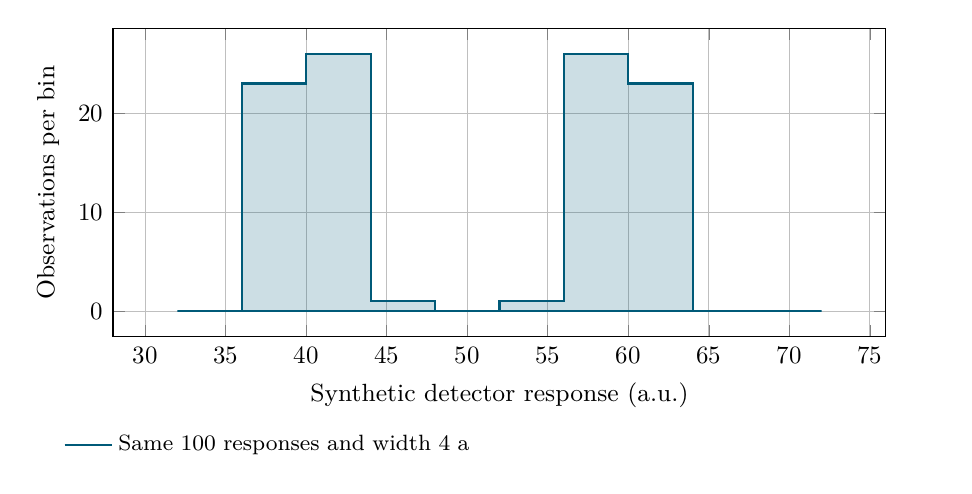
\begin{tikzpicture}
\begin{axis}[width=0.94\linewidth,
height=5.5cm,
scale only axis=false,
grid=major,
tick label style={font=\small},
label style={font=\small},
xlabel={Synthetic detector response (a.u.)},
ylabel={Observations per bin},
legend style={font=\footnotesize,draw=none,at={(0.5,-0.28)},anchor=north,legend columns=1,text width=0.85\linewidth,align=left},
unbounded coords=jump,
scaled ticks=false]
\addplot[color=pcd1,thick,mark=none,fill=pcd1,fill opacity=0.2] coordinates {(32,0) (32,0) (36,0) (36,23) (40,23) (40,26) (44,26) (44,1) (48,1) (48,0) (52,0) (52,1) (56,1) (56,26) (60,26) (60,23) (64,23) (64,0) (68,0) (68,0) (72,0) (72,0)} \closedcycle;
\addlegendentry{Same 100 responses and width 4 a}

\end{axis}
\end{tikzpicture}
\end{center}

\medskip

The rules in \hyperref[material-b79fa2ec639a26efd498b4dc6f4f0826a8732260ccc70b81ddc8c91803f5e8ee]{Eq.~\ref*{material-b79fa2ec639a26efd498b4dc6f4f0826a8732260ccc70b81ddc8c91803f5e8ee}} provide reproducible starting widths, using the sample size and the authored spread summaries. The adjustable example in \hyperref[material-d9622bef2398d02aee45c03e28989c345be821626ca37eb7ed08140e1afad58f]{Fig.~\ref*{material-d9622bef2398d02aee45c03e28989c345be821626ca37eb7ed08140e1afad58f}} supports checking those choices against the observations. A reported histogram therefore identifies the quantity, units, vertical-axis normalization and interval construction. Its interpretation can then focus on features that remain meaningful at the chosen resolution.


\par\medskip
\noindent\begin{minipage}{\linewidth}
\refstepcounter{equation}\label{material-b79fa2ec639a26efd498b4dc6f4f0826a8732260ccc70b81ddc8c91803f5e8ee}
\noindent\textbf{Eq.~\ref*{material-b79fa2ec639a26efd498b4dc6f4f0826a8732260ccc70b81ddc8c91803f5e8ee}.} Authored histogram-width rules with sample-size, spread and unit conventions.\par\nopagebreak
\begin{center}\begin{adjustbox}{max width=\linewidth}$\displaystyle \begin{gathered}h_{FD}=2\,\mathrm{IQR}\,n^{-1/3}\\h_{Scott}=3.5\,s\,n^{-1/3}\\k_{Sturges}=\lceil1+\log_2 n\rceil\end{gathered}$\end{adjustbox}\end{center}

\par\noindent\textbf{Symbols}

\par\noindent\textbf{Names and symbols} FD = Freedman–Diaconis; Scott = Scott's rule; Sturges = Sturges' rule. h: width; k: bin count; n: observations; s: sample SD. IQR uses linear interpolation.

\end{minipage}\par
\medskip

\par\medskip
\Needspace{10cm}
\refstepcounter{figure}\label{material-d9622bef2398d02aee45c03e28989c345be821626ca37eb7ed08140e1afad58f}
\noindent\textbf{Fig.~\ref*{material-d9622bef2398d02aee45c03e28989c345be821626ca37eb7ed08140e1afad58f}.} Adjustable histogram at its authored reference settings; the interactive view retains the available parameters.\par\nopagebreak
\begin{center}
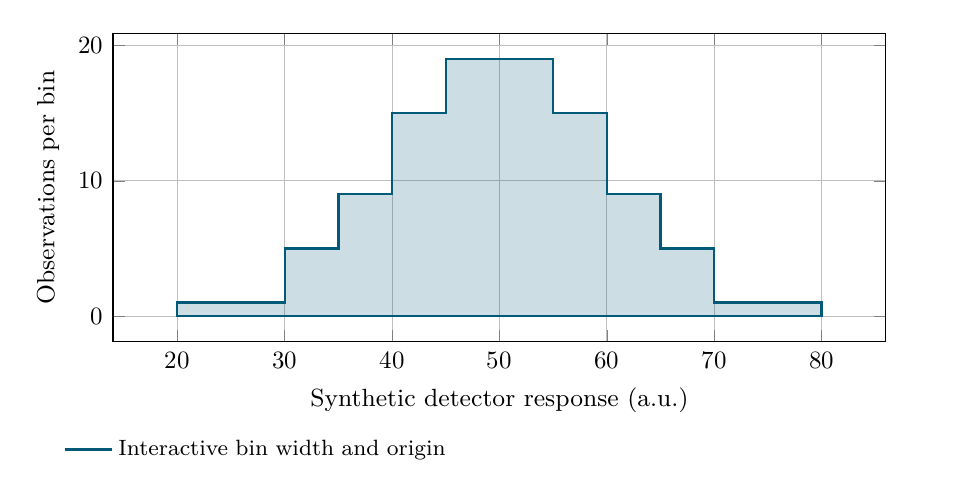
\begin{tikzpicture}
\begin{axis}[width=0.94\linewidth,
height=5.5cm,
scale only axis=false,
grid=major,
tick label style={font=\small},
label style={font=\small},
xlabel={Synthetic detector response (a.u.)},
ylabel={Observations per bin},
legend style={font=\footnotesize,draw=none,at={(0.5,-0.28)},anchor=north,legend columns=1,text width=0.85\linewidth,align=left},
unbounded coords=jump,
scaled ticks=false]
\addplot[color=pcd1,thick,mark=none,fill=pcd1,fill opacity=0.2] coordinates {(20,0) (20,1) (25,1) (25,1) (30,1) (30,5) (35,5) (35,9) (40,9) (40,15) (45,15) (45,19) (50,19) (50,19) (55,19) (55,15) (60,15) (60,9) (65,9) (65,5) (70,5) (70,1) (75,1) (75,1) (80,1) (80,0)} \closedcycle;
\addlegendentry{Interactive bin width and origin}

\end{axis}
\end{tikzpicture}
\end{center}

\medskip

\clearpage
\section{For unequal widths, area carries the relative frequency}
Unequal-width intervals make the distinction between bar height and bar area essential. The density-height formula in \hyperref[material-03550a8f6166842478e9074a2f3ee2081f921a70e5093cc28d7700fcc2ad0c99]{Eq.~\ref*{material-03550a8f6166842478e9074a2f3ee2081f921a70e5093cc28d7700fcc2ad0c99}} divides relative frequency by interval width. Multiplying that height by its width recovers the fraction of observations in the bin. Density consequently has reciprocal measurement units, while relative frequency is dimensionless.


\par\medskip
\noindent\begin{minipage}{\linewidth}
\refstepcounter{equation}\label{material-03550a8f6166842478e9074a2f3ee2081f921a70e5093cc28d7700fcc2ad0c99}
\noindent\textbf{Eq.~\ref*{material-03550a8f6166842478e9074a2f3ee2081f921a70e5093cc28d7700fcc2ad0c99}.} Density normalization for unequal-width histogram intervals: bar area equals observed relative frequency.\par\nopagebreak
\begin{center}\begin{adjustbox}{max width=\linewidth}$\displaystyle \begin{gathered}h_j=b_{j+1}-b_j\\d_j=\frac{n_j}{n\,h_j}\\d_jh_j=\frac{n_j}{n},\qquad\sum_j d_jh_j=1\end{gathered}$\end{adjustbox}\end{center}

\par\noindent\textbf{Symbols}

\par\noindent\textbf{Reading the symbols} b: edges; h\ensuremath{{}_j}: bin width; n\ensuremath{{}_j}: count; n: total. Density has inverse measurement units; bar area is the sample fraction.

\end{minipage}\par
\medskip

The unequal-bin construction in \hyperref[material-b614f62b2eafbd0aaecc0ae2f10da62b3035240be66c834f44e5012c8e11e9e3]{Fig.~\ref*{material-b614f62b2eafbd0aaecc0ae2f10da62b3035240be66c834f44e5012c8e11e9e3}} and the adaptive example in \hyperref[material-b3f7299366b89aa2d9ee4755fe0d545b0737780ebd1ecaa62684ad487a5394e6]{Fig.~\ref*{material-b3f7299366b89aa2d9ee4755fe0d545b0737780ebd1ecaa62684ad487a5394e6}} retain the authored boundaries and observations. A narrow interval containing the same fraction as a wider interval requires a taller density bar. This relationship explains why reading the vertical-axis label is part of reading the distribution.


\par\medskip
\Needspace{10cm}
\refstepcounter{figure}\label{material-b614f62b2eafbd0aaecc0ae2f10da62b3035240be66c834f44e5012c8e11e9e3}
\noindent\textbf{Fig.~\ref*{material-b614f62b2eafbd0aaecc0ae2f10da62b3035240be66c834f44e5012c8e11e9e3}.} Authored unequal-width bins with density heights corresponding to their observed fractions.\par\nopagebreak
\begin{center}
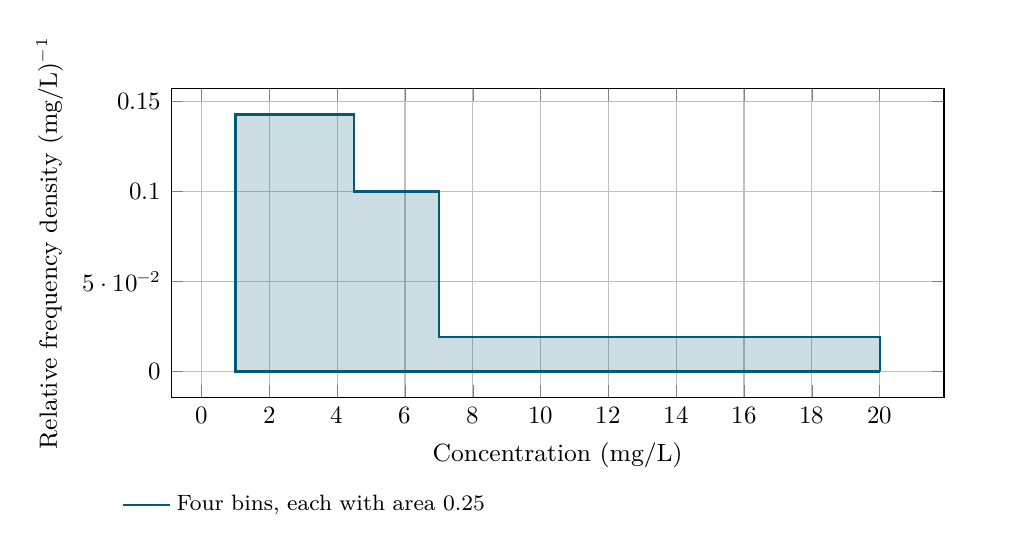
\begin{tikzpicture}
\begin{axis}[width=0.94\linewidth,
height=5.5cm,
scale only axis=false,
grid=major,
tick label style={font=\small},
label style={font=\small},
xlabel={Concentration (mg/L)},
ylabel={Relative frequency density (mg/L)\ensuremath{{}^-}\ensuremath{{}^1}},
legend style={font=\footnotesize,draw=none,at={(0.5,-0.28)},anchor=north,legend columns=1,text width=0.85\linewidth,align=left},
unbounded coords=jump,
scaled ticks=false]
\addplot[color=pcd1,thick,mark=none,fill=pcd1,fill opacity=0.2] coordinates {(1,0) (1,0.14285714285714285) (2.75,0.14285714285714285) (2.75,0.14285714285714285) (4.5,0.14285714285714285) (4.5,0.1) (7,0.1) (7,0.019230769230769232) (20,0.019230769230769232) (20,0)} \closedcycle;
\addlegendentry{Four bins, each with area 0.25}

\end{axis}
\end{tikzpicture}
\end{center}

\medskip

\par\medskip
\Needspace{10cm}
\refstepcounter{figure}\label{material-b3f7299366b89aa2d9ee4755fe0d545b0737780ebd1ecaa62684ad487a5394e6}
\noindent\textbf{Fig.~\ref*{material-b3f7299366b89aa2d9ee4755fe0d545b0737780ebd1ecaa62684ad487a5394e6}.} Adaptive-width histogram at the authored interval settings and density normalization.\par\nopagebreak
\begin{center}
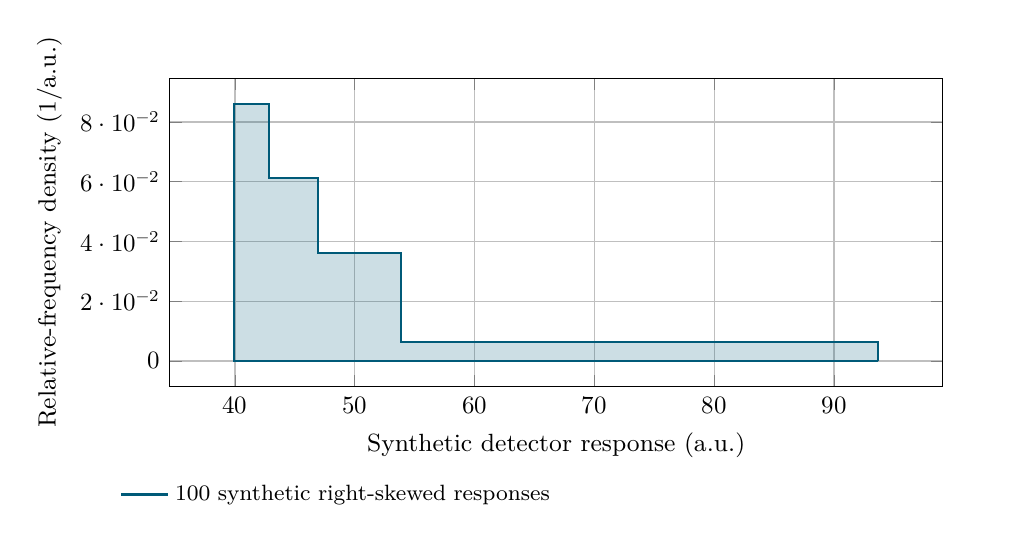
\begin{tikzpicture}
\begin{axis}[width=0.94\linewidth,
height=5.5cm,
scale only axis=false,
grid=major,
tick label style={font=\small},
label style={font=\small},
xlabel={Synthetic detector response (a.u.)},
ylabel={Relative-frequency density (1/a.u.)},
legend style={font=\footnotesize,draw=none,at={(0.5,-0.28)},anchor=north,legend columns=1,text width=0.85\linewidth,align=left},
unbounded coords=jump,
scaled ticks=false]
\addplot[color=pcd1,thick,mark=none,fill=pcd1,fill opacity=0.2] coordinates {(39.930215496246,0) (39.930215496246,0.08606363585086985) (42.8350428083665,0.08606363585086985) (42.8350428083665,0.06121044719183694) (46.9193129202395,0.06121044719183694) (46.9193129202395,0.036025920418367746) (53.85876088150624,0.036025920418367746) (53.85876088150624,0.006276763382805469) (93.688205573471,0.006276763382805469) (93.688205573471,0)} \closedcycle;
\addlegendentry{100 synthetic right-skewed responses}

\end{axis}
\end{tikzpicture}
\end{center}

\medskip

The two-dimensional histogram in \hyperref[material-9e9bc76ff0e99d10eb6c2e5a8b2ee6a0c386f609d44164c039ba870026fae7fd]{Fig.~\ref*{material-9e9bc76ff0e99d10eb6c2e5a8b2ee6a0c386f609d44164c039ba870026fae7fd}} extends grouping to pairs of variables and a grid of cells. Its normalization follows the authored count or density convention. The optional R source in \hyperref[material-5babe8df6ccf8bc08ac579b4e1dc6435dc98a334cbae4e495c1f0b4a68b91f8f]{Listing~\ref*{material-5babe8df6ccf8bc08ac579b4e1dc6435dc98a334cbae4e495c1f0b4a68b91f8f}} reproduces the histogram examples and their settings. Together these views support a consistent question: which proportion of the observed sample occupies a specified region of the measurement space?


\par\medskip
\Needspace{10cm}
\refstepcounter{figure}\label{material-9e9bc76ff0e99d10eb6c2e5a8b2ee6a0c386f609d44164c039ba870026fae7fd}
\noindent\textbf{Fig.~\ref*{material-9e9bc76ff0e99d10eb6c2e5a8b2ee6a0c386f609d44164c039ba870026fae7fd}.} Two-dimensional histogram of the authored paired observations and cell-normalization convention.\par\nopagebreak
\begin{center}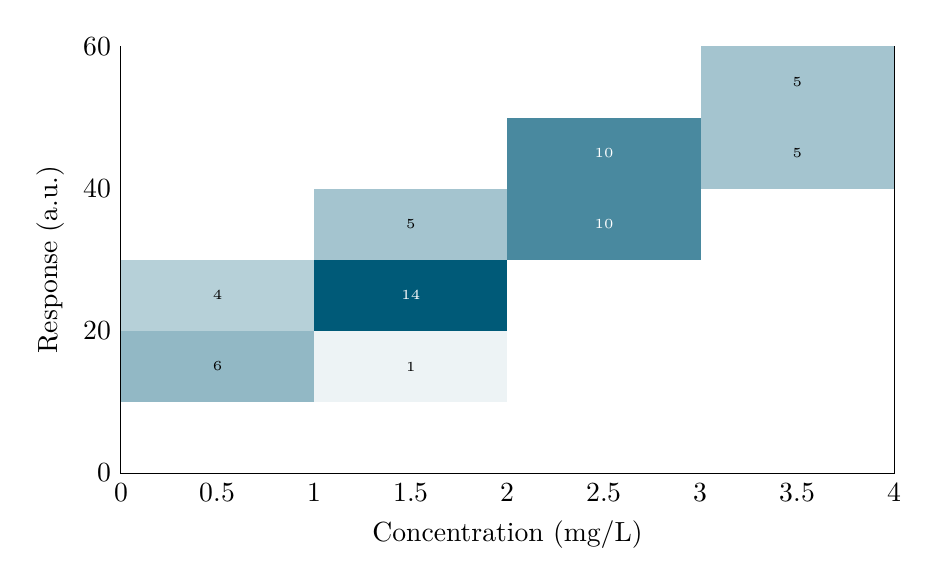
\begin{tikzpicture}\begin{axis}[width=.94\linewidth,height=7cm,xlabel={Concentration (mg/L)},ylabel={Response (a.u.)},xmin=0,xmax=4,ymin=0,ymax=60]
\path[fill=pcd1!0] (axis cs:0,0) rectangle (axis cs:1,10);
\path[fill=pcd1!0] (axis cs:1,0) rectangle (axis cs:2,10);
\path[fill=pcd1!0] (axis cs:2,0) rectangle (axis cs:3,10);
\path[fill=pcd1!0] (axis cs:3,0) rectangle (axis cs:4,10);
\path[fill=pcd1!42.857142857142854] (axis cs:0,10) rectangle (axis cs:1,20);\node[font=\tiny,text=black] at (axis cs:0.5,15) {6};
\path[fill=pcd1!7.142857142857143] (axis cs:1,10) rectangle (axis cs:2,20);\node[font=\tiny,text=black] at (axis cs:1.5,15) {1};
\path[fill=pcd1!0] (axis cs:2,10) rectangle (axis cs:3,20);
\path[fill=pcd1!0] (axis cs:3,10) rectangle (axis cs:4,20);
\path[fill=pcd1!28.571428571428573] (axis cs:0,20) rectangle (axis cs:1,30);\node[font=\tiny,text=black] at (axis cs:0.5,25) {4};
\path[fill=pcd1!100] (axis cs:1,20) rectangle (axis cs:2,30);\node[font=\tiny,text=white] at (axis cs:1.5,25) {14};
\path[fill=pcd1!0] (axis cs:2,20) rectangle (axis cs:3,30);
\path[fill=pcd1!0] (axis cs:3,20) rectangle (axis cs:4,30);
\path[fill=pcd1!0] (axis cs:0,30) rectangle (axis cs:1,40);
\path[fill=pcd1!35.714285714285715] (axis cs:1,30) rectangle (axis cs:2,40);\node[font=\tiny,text=black] at (axis cs:1.5,35) {5};
\path[fill=pcd1!71.42857142857143] (axis cs:2,30) rectangle (axis cs:3,40);\node[font=\tiny,text=white] at (axis cs:2.5,35) {10};
\path[fill=pcd1!0] (axis cs:3,30) rectangle (axis cs:4,40);
\path[fill=pcd1!0] (axis cs:0,40) rectangle (axis cs:1,50);
\path[fill=pcd1!0] (axis cs:1,40) rectangle (axis cs:2,50);
\path[fill=pcd1!71.42857142857143] (axis cs:2,40) rectangle (axis cs:3,50);\node[font=\tiny,text=white] at (axis cs:2.5,45) {10};
\path[fill=pcd1!35.714285714285715] (axis cs:3,40) rectangle (axis cs:4,50);\node[font=\tiny,text=black] at (axis cs:3.5,45) {5};
\path[fill=pcd1!0] (axis cs:0,50) rectangle (axis cs:1,60);
\path[fill=pcd1!0] (axis cs:1,50) rectangle (axis cs:2,60);
\path[fill=pcd1!0] (axis cs:2,50) rectangle (axis cs:3,60);
\path[fill=pcd1!35.714285714285715] (axis cs:3,50) rectangle (axis cs:4,60);\node[font=\tiny,text=black] at (axis cs:3.5,55) {5};
\end{axis}\end{tikzpicture}\end{center}
\noindent Cell labels give observation counts.

\medskip

\par\medskip
\Needspace{8\baselineskip}
\refstepcounter{listing}\label{material-5babe8df6ccf8bc08ac579b4e1dc6435dc98a334cbae4e495c1f0b4a68b91f8f}
\noindent\textbf{Listing~\ref*{material-5babe8df6ccf8bc08ac579b4e1dc6435dc98a334cbae4e495c1f0b4a68b91f8f}.} Optional R source for the histogram laboratory, including the authored data and bin choices.\par\nopagebreak
\begin{Verbatim}[fontsize=\footnotesize,breaklines=true,breakanywhere=true]
if (!requireNamespace("ggplot2", quietly = TRUE)) {
  if (requireNamespace("webr", quietly = TRUE)) webr::install("ggplot2")
  else stop("Install ggplot2 first")
}
library(ggplot2)
x <- c(
  36.203861904595, 36.968344965996, 37.373171342811, 37.663249348955, 37.894944427129, 38.090935235275, 38.262750520860, 38.417100222768, 38.558256085355, 38.689118543731,
  38.811755599904, 38.927699911254, 39.038123973652, 39.143949102676, 39.245916271163, 39.344633882841, 39.440611031230, 39.534281313527, 39.626020324213, 39.716158820762,
  39.804992871389, 39.892791871197, 39.979805043931, 40.066266872452, 40.152401787581, 40.238428371541, 40.324563286669, 40.411025115191, 40.498038287925, 40.585837287733,
  40.674671338359, 40.764809834908, 40.856548845594, 40.950219127892, 41.046196276280, 41.144913887958, 41.246881056446, 41.352706185469, 41.463130247867, 41.579074559217,
  41.701711615390, 41.832574073766, 41.973729936353, 42.128079638261, 42.299894923847, 42.495885731992, 42.727580810167, 43.017658816310, 43.422485193125, 44.186968254526,
  55.813031745474, 56.577514806875, 56.982341183690, 57.272419189833, 57.504114268008, 57.700105076153, 57.871920361739, 58.026270063647, 58.167425926234, 58.298288384610,
  58.420925440783, 58.536869752133, 58.647293814531, 58.753118943554, 58.855086112042, 58.953803723720, 59.049780872108, 59.143451154406, 59.235190165092, 59.325328661641,
  59.414162712267, 59.501961712075, 59.588974884809, 59.675436713331, 59.761571628459, 59.847598212419, 59.933733127548, 60.020194956069, 60.107208128803, 60.195007128611,
  60.283841179238, 60.373979675787, 60.465718686473, 60.559388968770, 60.655366117159, 60.754083728837, 60.856050897324, 60.961876026348, 61.072300088746, 61.188244400096,
  61.310881456269, 61.441743914645, 61.582899777232, 61.737249479140, 61.909064764725, 62.105055572871, 62.336750651045, 62.626828657189, 63.031655034004, 63.796138095405
)
bin_width <- 4
p <- ggplot(data.frame(x), aes(x)) +
  geom_histogram(breaks = seq(30, 70, by = bin_width), closed = "left") +
  labs(x = "Synthetic detector response (a.u.)", y = "Count") +
  theme_minimal(base_size = 16)
print(p)
b <- ggplot_build(p)$data[[1]]
b[c("xmin", "xmax", "count", "density")]
sum(b$count)
\end{Verbatim}

\par\noindent\textbf{geom\_histogram(breaks=..., closed="left")}

Specify numeric edges and interval closure explicitly, then verify that the bins cover and count every observation.

\par\noindent\textbf{ggplot\_build(p)\$data[[1]]}

Inspect xmin/xmax, count and density; verify sum(count)=length(x).

\par\noindent\textbf{ggplot(..., aes(x))}

\textbf{ggplot()} creates the plot; \textbf{aes(x)} maps the observation column to the horizontal axis. The histogram layer computes counts.

\par\noindent\textbf{c(...)}

Combine the supplied responses or the selected output-column names into a vector.

\par\noindent\textbf{data.frame(x)}

Put the response vector into a named table column for ggplot.

\par\noindent\textbf{seq(30, 70, by=bin\_width)}

Generate \textbf{explicit bin edges}. Changing bin\_width changes these edges, not the observations.

\par\noindent\textbf{sum(b\$count)}

Add all bin counts. \textbf{Check against 100} so observations do not silently disappear outside the edges.

\par\noindent\textbf{requireNamespace(..., quietly=TRUE)}

Check package availability without attaching it; the logical result selects the setup branch.

\par\noindent\textbf{webr::install("ggplot2")}

Download ggplot2 into browser R if missing. \textbf{Network required}, not an upload of learner observations.

\par\noindent\textbf{stop(...)}

Stop with an explanatory setup error. Desktop R needs ggplot2 installed separately.

\par\noindent\textbf{library(ggplot2)}

Attach the installed plotting package so its functions are available by name.

\par\noindent\textbf{print(p)}

Draw the histogram explicitly in the browser R runtime.

\par\noindent\textbf{labs(x=..., y=...)}

Label the measurement axis with its unit and the vertical axis as \textbf{Count}.

\par\noindent\textbf{theme\_minimal(base\_size=16)}

Set the plot theme and font size; the bin counts do not change.

\par\noindent\textbf{<-, \$, [, [[, +, if / else, ! and ::}

\textbf{<-} assigns; \textbf{\$} selects a column; \textbf{[} subsets; \textbf{[[} extracts a list element. \textbf{+} adds plot layers; \textbf{if/else} branches; \textbf{!} negates; \textbf{::} selects a package function.

\medskip

\clearpage
\section{An empirical CDF answers cumulative threshold questions directly}
Many analytical questions ask what fraction of observations is at or below a concentration threshold. The empirical cumulative distribution function in \hyperref[material-8e803ae2a6b4cdc628ff61c21875781b3ae510871c1c2419514dd715db723544]{Eq.~\ref*{material-8e803ae2a6b4cdc628ff61c21875781b3ae510871c1c2419514dd715db723544}} calculates that fraction for every threshold. Each observed value adds its share to the cumulative total, and tied values produce a combined jump. The definition specifies the inclusive threshold convention.


\par\medskip
\noindent\begin{minipage}{\linewidth}
\refstepcounter{equation}\label{material-8e803ae2a6b4cdc628ff61c21875781b3ae510871c1c2419514dd715db723544}
\noindent\textbf{Eq.~\ref*{material-8e803ae2a6b4cdc628ff61c21875781b3ae510871c1c2419514dd715db723544}.} Empirical CDF with the inclusive threshold, indicator, sample-size and tie conventions.\par\nopagebreak
\begin{center}\begin{adjustbox}{max width=\linewidth}$\displaystyle F_n(x)=\frac1n\sum_{i=1}^{n}\mathbf{1}\{x_i\le x\}$\end{adjustbox}\end{center}

\par\noindent\textbf{Symbols}

\par\noindent\textbf{F\ensuremath{{}_n}(x) and x} F\ensuremath{{}_n}(x): unitless sample fraction at or below threshold x. The threshold x has the measurement unit.

\par\noindent\textbf{x\ensuremath{{}_i}, n, i and \ensuremath{\Sigma}} x\ensuremath{{}_i}: observed value i; n: sample size; i: index 1 to n; \ensuremath{\Sigma}: sum over every observation, including ties.

\par\noindent\textbf{1\{x\ensuremath{{}_i} \ensuremath{\le} x\}} Indicator: 1 when x\ensuremath{{}_i} \ensuremath{\le} x, otherwise 0. Equality is included: tied values enter together. Dividing the count by n gives the fraction.

\end{minipage}\par
\medskip

The small worked example in \hyperref[material-74e6eb1f08c991787d97767686d06f23075387f292493789e5ba3a020a77ad0e]{Fig.~\ref*{material-74e6eb1f08c991787d97767686d06f23075387f292493789e5ba3a020a77ad0e}} makes the counting operation visible. The river example in \hyperref[material-cf926440e0f185a3dba9330ea73d226a9dcd260d7e2299f87030966561a350a7]{Fig.~\ref*{material-cf926440e0f185a3dba9330ea73d226a9dcd260d7e2299f87030966561a350a7}} gives it an analytical interpretation: read horizontally from a concentration to obtain the observed fraction, or start from a cumulative level to locate an empirical threshold under the stated quantile convention. The observations remain the basis for both readings.


\par\medskip
\Needspace{10cm}
\refstepcounter{figure}\label{material-74e6eb1f08c991787d97767686d06f23075387f292493789e5ba3a020a77ad0e}
\noindent\textbf{Fig.~\ref*{material-74e6eb1f08c991787d97767686d06f23075387f292493789e5ba3a020a77ad0e}.} Worked empirical cumulative steps for the authored small sample.\par\nopagebreak
\begin{center}
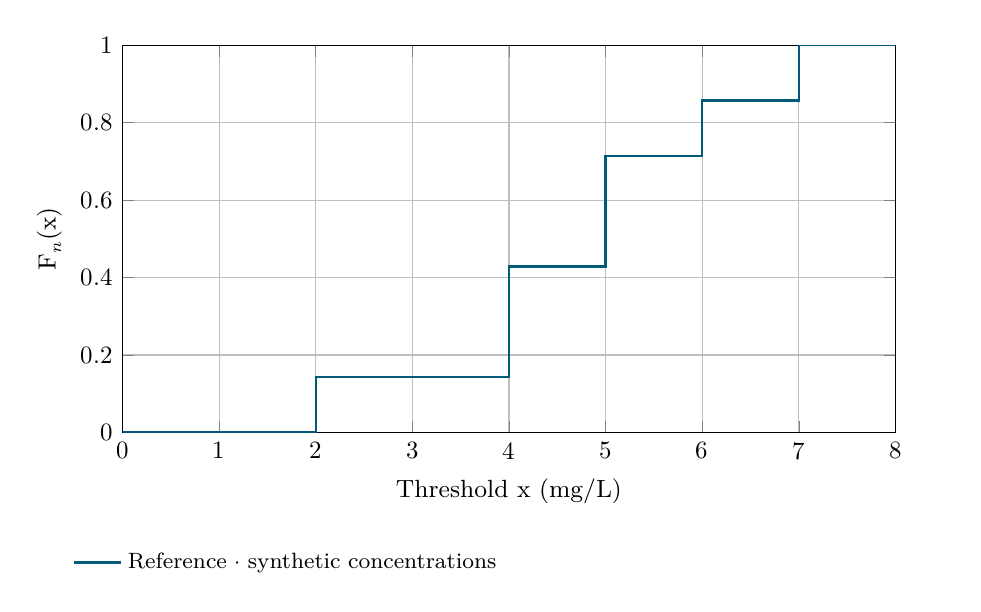
\begin{tikzpicture}
\begin{axis}[width=0.94\linewidth,
height=6.5cm,
scale only axis=false,
grid=major,
tick label style={font=\small},
label style={font=\small},
xlabel={Threshold x (mg/L)},
ylabel={F\ensuremath{{}_n}(x)},
legend style={font=\footnotesize,draw=none,at={(0.5,-0.28)},anchor=north,legend columns=1,text width=0.85\linewidth,align=left},
unbounded coords=jump,
scaled ticks=false,
ymin=0,
ymax=1,
xmin=0,
xmax=8]
\addplot[color=pcd1,thick,mark=none] coordinates {(0,0) (2,0) (2,0.14285714285714285) (4,0.14285714285714285) (4,0.42857142857142855) (5,0.42857142857142855) (5,0.7142857142857143) (6,0.7142857142857143) (6,0.8571428571428571) (7,0.8571428571428571) (7,1) (8,1)};
\addlegendentry{Reference \ensuremath{\cdot} synthetic concentrations}

\end{axis}
\end{tikzpicture}
\end{center}

\medskip

\par\medskip
\Needspace{10cm}
\refstepcounter{figure}\label{material-cf926440e0f185a3dba9330ea73d226a9dcd260d7e2299f87030966561a350a7}
\noindent\textbf{Fig.~\ref*{material-cf926440e0f185a3dba9330ea73d226a9dcd260d7e2299f87030966561a350a7}.} River-concentration ECDF for cumulative-threshold and empirical-quantile readings.\par\nopagebreak
\begin{center}
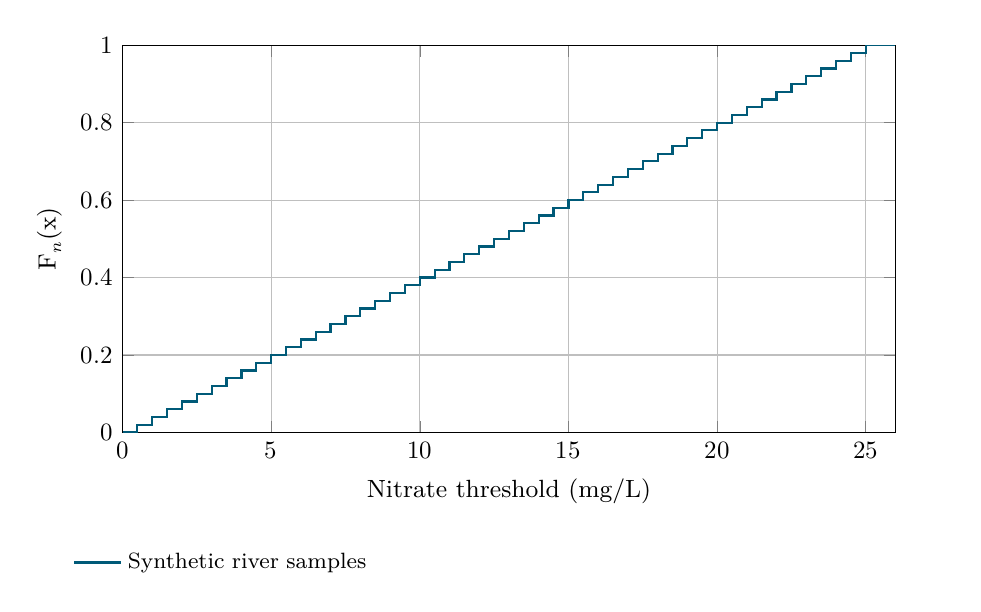
\begin{tikzpicture}
\begin{axis}[width=0.94\linewidth,
height=6.5cm,
scale only axis=false,
grid=major,
tick label style={font=\small},
label style={font=\small},
xlabel={Nitrate threshold (mg/L)},
ylabel={F\ensuremath{{}_n}(x)},
legend style={font=\footnotesize,draw=none,at={(0.5,-0.28)},anchor=north,legend columns=1,text width=0.85\linewidth,align=left},
unbounded coords=jump,
scaled ticks=false,
ymin=0,
ymax=1,
xmin=0,
xmax=26]
\addplot[color=pcd1,thick,mark=none] coordinates {(0,0) (0.5,0) (0.5,0.02) (1,0.02) (1,0.04) (1.5,0.04) (1.5,0.06) (2,0.06) (2,0.08) (2.5,0.08) (2.5,0.1) (3,0.1) (3,0.12) (3.5,0.12) (3.5,0.14) (4,0.14) (4,0.16) (4.5,0.16) (4.5,0.18) (5,0.18) (5,0.2) (5.5,0.2) (5.5,0.22) (6,0.22) (6,0.24) (6.5,0.24) (6.5,0.26) (7,0.26) (7,0.28) (7.5,0.28) (7.5,0.3) (8,0.3) (8,0.32) (8.5,0.32) (8.5,0.34) (9,0.34) (9,0.36) (9.5,0.36) (9.5,0.38) (10,0.38) (10,0.4) (10.5,0.4) (10.5,0.42) (11,0.42) (11,0.44) (11.5,0.44) (11.5,0.46) (12,0.46) (12,0.48) (12.5,0.48) (12.5,0.5) (13,0.5) (13,0.52) (13.5,0.52) (13.5,0.54) (14,0.54) (14,0.56) (14.5,0.56) (14.5,0.58) (15,0.58) (15,0.6) (15.5,0.6) (15.5,0.62) (16,0.62) (16,0.64) (16.5,0.64) (16.5,0.66) (17,0.66) (17,0.68) (17.5,0.68) (17.5,0.7) (18,0.7) (18,0.72) (18.5,0.72) (18.5,0.74) (19,0.74) (19,0.76) (19.5,0.76) (19.5,0.78) (20,0.78) (20,0.8) (20.5,0.8) (20.5,0.82) (21,0.82) (21,0.84) (21.5,0.84) (21.5,0.86) (22,0.86) (22,0.88) (22.5,0.88) (22.5,0.9) (23,0.9) (23,0.92) (23.5,0.92) (23.5,0.94) (24,0.94) (24,0.96) (24.5,0.96) (24.5,0.98) (25,0.98) (25,1) (26,1)};
\addlegendentry{Synthetic river samples}

\end{axis}
\end{tikzpicture}
\end{center}

\medskip

The shape comparison in \hyperref[material-a2f699dff2b41e1826adcca39ff35a9c7388c0af2cc15bfc67d2bd14b80953e2]{Fig.~\ref*{material-a2f699dff2b41e1826adcca39ff35a9c7388c0af2cc15bfc67d2bd14b80953e2}} uses cumulative curves to compare complete empirical distributions. A curve lying higher at a fixed concentration represents a larger observed fraction below that concentration. Crossing curves show that the ordering depends on the threshold. Generalizing these empirical comparisons to populations additionally requires an inferential model and a sampling design appropriate to the question.


\par\medskip
\Needspace{10cm}
\refstepcounter{figure}\label{material-a2f699dff2b41e1826adcca39ff35a9c7388c0af2cc15bfc67d2bd14b80953e2}
\noindent\textbf{Fig.~\ref*{material-a2f699dff2b41e1826adcca39ff35a9c7388c0af2cc15bfc67d2bd14b80953e2}.} Empirical cumulative comparison of the authored distribution shapes, including threshold-dependent curve orderings.\par\nopagebreak
\begin{center}
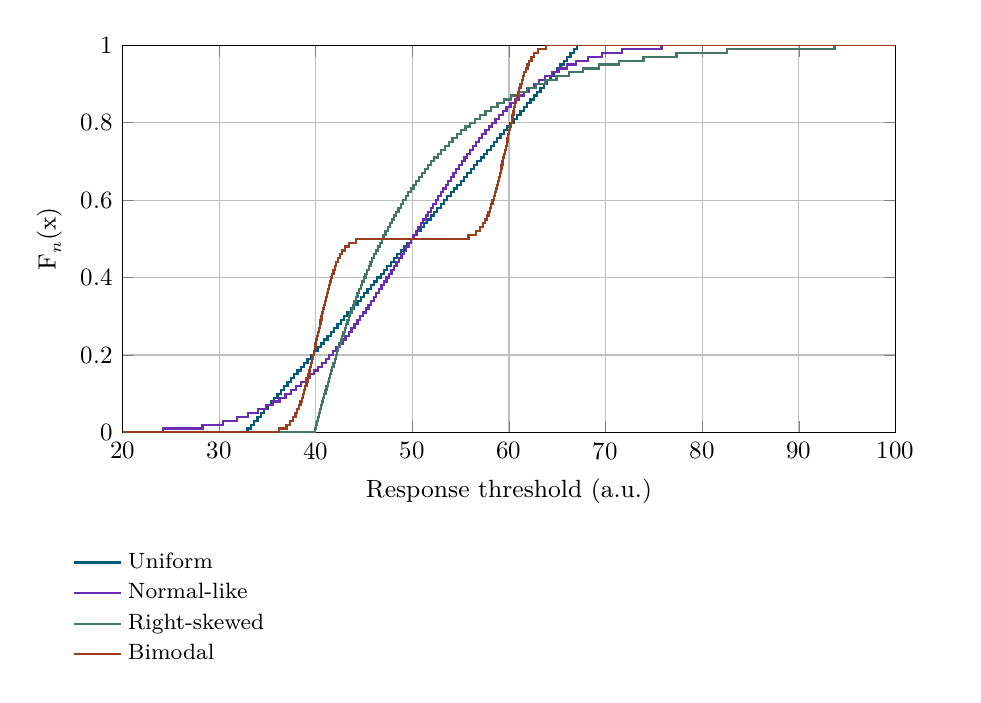
\begin{tikzpicture}
\begin{axis}[width=0.94\linewidth,
height=6.5cm,
scale only axis=false,
grid=major,
tick label style={font=\small},
label style={font=\small},
xlabel={Response threshold (a.u.)},
ylabel={F\ensuremath{{}_n}(x)},
legend style={font=\footnotesize,draw=none,at={(0.5,-0.28)},anchor=north,legend columns=1,text width=0.85\linewidth,align=left},
unbounded coords=jump,
scaled ticks=false,
ymin=0,
ymax=1,
xmin=20,
xmax=100]
\addplot[color=pcd1,thick,mark=none] coordinates {(20,0) (32.937795808244,0) (32.937795808244,0.01) (33.282486802016,0.01) (33.282486802016,0.02) (33.627177795789,0.02) (33.627177795789,0.03) (33.971868789562,0.03) (33.971868789562,0.04) (34.316559783335,0.04) (34.316559783335,0.05) (34.661250777108,0.05) (34.661250777108,0.06) (35.005941770881,0.06) (35.005941770881,0.07) (35.350632764654,0.07) (35.350632764654,0.08) (35.695323758426,0.08) (35.695323758426,0.09) (36.040014752199,0.09) (36.040014752199,0.1) (36.384705745972,0.1) (36.384705745972,0.11) (36.729396739745,0.11) (36.729396739745,0.12) (37.074087733518,0.12) (37.074087733518,0.13) (37.418778727291,0.13) (37.418778727291,0.14) (37.763469721064,0.14) (37.763469721064,0.15) (38.108160714836,0.15) (38.108160714836,0.16) (38.452851708609,0.16) (38.452851708609,0.17) (38.797542702382,0.17) (38.797542702382,0.18) (39.142233696155,0.18) (39.142233696155,0.19) (39.486924689928,0.19) (39.486924689928,0.2) (39.831615683701,0.2) (39.831615683701,0.21) (40.176306677474,0.21) (40.176306677474,0.22) (40.520997671246,0.22) (40.520997671246,0.23) (40.865688665019,0.23) (40.865688665019,0.24) (41.210379658792,0.24) (41.210379658792,0.25) (41.555070652565,0.25) (41.555070652565,0.26) (41.899761646338,0.26) (41.899761646338,0.27) (42.244452640111,0.27) (42.244452640111,0.28) (42.589143633884,0.28) (42.589143633884,0.29) (42.933834627656,0.29) (42.933834627656,0.3) (43.278525621429,0.3) (43.278525621429,0.31) (43.623216615202,0.31) (43.623216615202,0.32) (43.967907608975,0.32) (43.967907608975,0.33) (44.312598602748,0.33) (44.312598602748,0.34) (44.657289596521,0.34) (44.657289596521,0.35) (45.001980590294,0.35) (45.001980590294,0.36) (45.346671584066,0.36) (45.346671584066,0.37) (45.691362577839,0.37) (45.691362577839,0.38) (46.036053571612,0.38) (46.036053571612,0.39) (46.380744565385,0.39) (46.380744565385,0.4) (46.725435559158,0.4) (46.725435559158,0.41) (47.070126552931,0.41) (47.070126552931,0.42) (47.414817546704,0.42) (47.414817546704,0.43) (47.759508540476,0.43) (47.759508540476,0.44) (48.104199534249,0.44) (48.104199534249,0.45) (48.448890528022,0.45) (48.448890528022,0.46) (48.793581521795,0.46) (48.793581521795,0.47) (49.138272515568,0.47) (49.138272515568,0.48) (49.482963509341,0.48) (49.482963509341,0.49) (49.827654503114,0.49) (49.827654503114,0.5) (50.172345496886,0.5) (50.172345496886,0.51) (50.517036490659,0.51) (50.517036490659,0.52) (50.861727484432,0.52) (50.861727484432,0.53) (51.206418478205,0.53) (51.206418478205,0.54) (51.551109471978,0.54) (51.551109471978,0.55) (51.895800465751,0.55) (51.895800465751,0.56) (52.240491459524,0.56) (52.240491459524,0.57) (52.585182453296,0.57) (52.585182453296,0.58) (52.929873447069,0.58) (52.929873447069,0.59) (53.274564440842,0.59) (53.274564440842,0.6) (53.619255434615,0.6) (53.619255434615,0.61) (53.963946428388,0.61) (53.963946428388,0.62) (54.308637422161,0.62) (54.308637422161,0.63) (54.653328415934,0.63) (54.653328415934,0.64) (54.998019409706,0.64) (54.998019409706,0.65) (55.342710403479,0.65) (55.342710403479,0.66) (55.687401397252,0.66) (55.687401397252,0.67) (56.032092391025,0.67) (56.032092391025,0.68) (56.376783384798,0.68) (56.376783384798,0.69) (56.721474378571,0.69) (56.721474378571,0.7) (57.066165372344,0.7) (57.066165372344,0.71) (57.410856366116,0.71) (57.410856366116,0.72) (57.755547359889,0.72) (57.755547359889,0.73) (58.100238353662,0.73) (58.100238353662,0.74) (58.444929347435,0.74) (58.444929347435,0.75) (58.789620341208,0.75) (58.789620341208,0.76) (59.134311334981,0.76) (59.134311334981,0.77) (59.479002328754,0.77) (59.479002328754,0.78) (59.823693322526,0.78) (59.823693322526,0.79) (60.168384316299,0.79) (60.168384316299,0.8) (60.513075310072,0.8) (60.513075310072,0.81) (60.857766303845,0.81) (60.857766303845,0.82) (61.202457297618,0.82) (61.202457297618,0.83) (61.547148291391,0.83) (61.547148291391,0.84) (61.891839285164,0.84) (61.891839285164,0.85) (62.236530278936,0.85) (62.236530278936,0.86) (62.581221272709,0.86) (62.581221272709,0.87) (62.925912266482,0.87) (62.925912266482,0.88) (63.270603260255,0.88) (63.270603260255,0.89) (63.615294254028,0.89) (63.615294254028,0.9) (63.959985247801,0.9) (63.959985247801,0.91) (64.304676241574,0.91) (64.304676241574,0.92) (64.649367235346,0.92) (64.649367235346,0.93) (64.994058229119,0.93) (64.994058229119,0.94) (65.338749222892,0.94) (65.338749222892,0.95) (65.683440216665,0.95) (65.683440216665,0.96) (66.028131210438,0.96) (66.028131210438,0.97) (66.372822204211,0.97) (66.372822204211,0.98) (66.717513197983,0.98) (66.717513197983,0.99) (67.062204191756,0.99) (67.062204191756,1) (100,1)};
\addlegendentry{Uniform}
\addplot[color=pcd2,thick,mark=none] coordinates {(20,0) (24.206635835883,0) (24.206635835883,0.01) (28.269549422019,0.01) (28.269549422019,0.02) (30.373674322229,0.02) (30.373674322229,0.03) (31.856223253642,0.03) (31.856223253642,0.04) (33.022939259286,0.04) (33.022939259286,0.05) (33.996308448767,0.05) (33.996308448767,0.06) (34.838365913792,0.06) (34.838365913792,0.07) (35.58508539193,0.07) (35.58508539193,0.08) (36.259278709141,0.08) (36.259278709141,0.09) (36.876364726706,0.09) (36.876364726706,0.1) (37.447277731692,0.1) (37.447277731692,0.11) (37.980067968729,0.11) (37.980067968729,0.12) (38.48084364786,0.12) (38.48084364786,0.13) (38.954355721997,0.13) (38.954355721997,0.14) (39.40437699918,0.14) (39.40437699918,0.15) (39.833956941897,0.15) (39.833956941897,0.16) (40.245598210373,0.16) (40.245598210373,0.17) (40.641382216077,0.17) (40.641382216077,0.18) (41.023060453084,0.18) (41.023060453084,0.19) (41.392122262472,0.19) (41.392122262472,0.2) (41.749845996961,0.2) (41.749845996961,0.21) (42.097338257528,0.21) (42.097338257528,0.22) (42.435564405174,0.22) (42.435564405174,0.23) (42.765372588295,0.23) (42.765372588295,0.24) (43.087512881045,0.24) (43.087512881045,0.25) (43.402652687281,0.25) (43.402652687281,0.26) (43.711389258082,0.26) (43.711389258082,0.27) (44.014259954043,0.27) (44.014259954043,0.28) (44.31175072803,0.28) (44.31175072803,0.29) (44.604303190988,0.29) (44.604303190988,0.3) (44.892320540063,0.3) (44.892320540063,0.31) (45.176172566306,0.31) (45.176172566306,0.32) (45.456199912458,0.32) (45.456199912458,0.33) (45.732717715837,0.33) (45.732717715837,0.34) (46.006018744083,0.34) (46.006018744083,0.35) (46.276376110428,0.35) (46.276376110428,0.36) (46.544045638705,0.36) (46.544045638705,0.37) (46.809267935405,0.37) (46.809267935405,0.38) (47.072270215874,0.38) (47.072270215874,0.39) (47.333267923585,0.39) (47.333267923585,0.4) (47.592466174974,0.4) (47.592466174974,0.41) (47.850061057056,0.41) (47.850061057056,0.42) (48.106240800864,0.42) (48.106240800864,0.43) (48.361186850331,0.43) (48.361186850331,0.44) (48.615074843483,0.44) (48.615074843483,0.45) (48.868075520607,0.45) (48.868075520607,0.46) (49.120355572217,0.46) (49.120355572217,0.47) (49.372078438265,0.47) (49.372078438265,0.48) (49.623405068846,0.48) (49.623405068846,0.49) (49.874494655831,0.49) (49.874494655831,0.5) (50.125505344169,0.5) (50.125505344169,0.51) (50.376594931154,0.51) (50.376594931154,0.52) (50.627921561735,0.52) (50.627921561735,0.53) (50.879644427783,0.53) (50.879644427783,0.54) (51.131924479393,0.54) (51.131924479393,0.55) (51.384925156517,0.55) (51.384925156517,0.56) (51.638813149669,0.56) (51.638813149669,0.57) (51.893759199136,0.57) (51.893759199136,0.58) (52.149938942944,0.58) (52.149938942944,0.59) (52.407533825026,0.59) (52.407533825026,0.6) (52.666732076415,0.6) (52.666732076415,0.61) (52.927729784126,0.61) (52.927729784126,0.62) (53.190732064595,0.62) (53.190732064595,0.63) (53.455954361295,0.63) (53.455954361295,0.64) (53.723623889572,0.64) (53.723623889572,0.65) (53.993981255917,0.65) (53.993981255917,0.66) (54.267282284163,0.66) (54.267282284163,0.67) (54.543800087542,0.67) (54.543800087542,0.68) (54.823827433694,0.68) (54.823827433694,0.69) (55.107679459937,0.69) (55.107679459937,0.7) (55.395696809012,0.7) (55.395696809012,0.71) (55.68824927197,0.71) (55.68824927197,0.72) (55.985740045957,0.72) (55.985740045957,0.73) (56.288610741918,0.73) (56.288610741918,0.74) (56.597347312719,0.74) (56.597347312719,0.75) (56.912487118955,0.75) (56.912487118955,0.76) (57.234627411705,0.76) (57.234627411705,0.77) (57.564435594826,0.77) (57.564435594826,0.78) (57.902661742472,0.78) (57.902661742472,0.79) (58.250154003039,0.79) (58.250154003039,0.8) (58.607877737528,0.8) (58.607877737528,0.81) (58.976939546916,0.81) (58.976939546916,0.82) (59.358617783923,0.82) (59.358617783923,0.83) (59.754401789627,0.83) (59.754401789627,0.84) (60.166043058103,0.84) (60.166043058103,0.85) (60.59562300082,0.85) (60.59562300082,0.86) (61.045644278003,0.86) (61.045644278003,0.87) (61.51915635214,0.87) (61.51915635214,0.88) (62.019932031271,0.88) (62.019932031271,0.89) (62.552722268308,0.89) (62.552722268308,0.9) (63.123635273294,0.9) (63.123635273294,0.91) (63.740721290859,0.91) (63.740721290859,0.92) (64.41491460807,0.92) (64.41491460807,0.93) (65.161634086208,0.93) (65.161634086208,0.94) (66.003691551233,0.94) (66.003691551233,0.95) (66.977060740714,0.95) (66.977060740714,0.96) (68.143776746358,0.96) (68.143776746358,0.97) (69.626325677771,0.97) (69.626325677771,0.98) (71.730450577981,0.98) (71.730450577981,0.99) (75.793364164117,0.99) (75.793364164117,1) (100,1)};
\addlegendentry{Normal-like}
\addplot[color=pcd3,thick,mark=none] coordinates {(20,0) (39.930215496246,0) (39.930215496246,0.01) (40.032800674276,0.01) (40.032800674276,0.02) (40.136432657911,0.02) (40.136432657911,0.03) (40.24113303134,0.03) (40.24113303134,0.04) (40.346924053282,0.04) (40.346924053282,0.05) (40.453828685386,0.05) (40.453828685386,0.06) (40.56187062215,0.06) (40.56187062215,0.07) (40.671074322438,0.07) (40.671074322438,0.08) (40.781465042716,0.08) (40.781465042716,0.09) (40.893068872116,0.09) (40.893068872116,0.1) (41.00591276944,0.1) (41.00591276944,0.11) (41.120024602253,0.11) (41.120024602253,0.12) (41.235433188192,0.12) (41.235433188192,0.13) (41.352168338646,0.13) (41.352168338646,0.14) (41.470260904983,0.14) (41.470260904983,0.15) (41.589742827495,0.15) (41.589742827495,0.16) (41.710647187247,0.16) (41.710647187247,0.17) (41.833008261065,0.17) (41.833008261065,0.18) (41.956861579865,0.18) (41.956861579865,0.19) (42.082243990591,0.19) (42.082243990591,0.2) (42.209193722015,0.2) (42.209193722015,0.21) (42.337750454712,0.21) (42.337750454712,0.22) (42.467955395514,0.22) (42.467955395514,0.23) (42.599851356805,0.23) (42.599851356805,0.24) (42.733482841024,0.24) (42.733482841024,0.25) (42.868896130814,0.25) (42.868896130814,0.26) (43.00613938525,0.26) (43.00613938525,0.27) (43.145262742673,0.27) (43.145262742673,0.28) (43.286318430648,0.28) (43.286318430648,0.29) (43.429360883685,0.29) (43.429360883685,0.3) (43.574446869357,0.3) (43.574446869357,0.31) (43.721635623558,0.31) (43.721635623558,0.32) (43.870988995719,0.32) (43.870988995719,0.33) (44.022571604848,0.33) (44.022571604848,0.34) (44.176451007399,0.34) (44.176451007399,0.35) (44.332697878059,0.35) (44.332697878059,0.36) (44.491386204653,0.36) (44.491386204653,0.37) (44.652593498525,0.37) (44.652593498525,0.38) (44.816401021887,0.38) (44.816401021887,0.39) (44.982894033802,0.39) (44.982894033802,0.4) (45.152162056669,0.4) (45.152162056669,0.41) (45.324299165303,0.41) (45.324299165303,0.42) (45.499404300925,0.42) (45.499404300925,0.43) (45.677581612709,0.43) (45.677581612709,0.44) (45.85894082983,0.44) (45.85894082983,0.45) (46.043597667329,0.45) (46.043597667329,0.46) (46.23167426958,0.46) (46.23167426958,0.47) (46.423299695584,0.47) (46.423299695584,0.48) (46.618610450948,0.48) (46.618610450948,0.49) (46.817751072022,0.49) (46.817751072022,0.5) (47.020874768457,0.5) (47.020874768457,0.51) (47.228144131353,0.51) (47.228144131353,0.52) (47.439731915181,0.52) (47.439731915181,0.53) (47.655821902906,0.53) (47.655821902906,0.54) (47.876609865167,0.54) (47.876609865167,0.55) (48.102304626062,0.55) (48.102304626062,0.56) (48.333129250065,0.56) (48.333129250065,0.57) (48.569322367003,0.57) (48.569322367003,0.58) (48.811139654802,0.58) (48.811139654802,0.59) (49.058855503111,0.59) (49.058855503111,0.6) (49.31276488494,0.6) (49.31276488494,0.61) (49.573185468321,0.61) (49.573185468321,0.62) (49.840460005917,0.62) (49.840460005917,0.63) (50.114959047658,0.63) (50.114959047658,0.64) (50.397084030267,0.64) (50.397084030267,0.65) (50.687270808317,0.65) (50.687270808317,0.66) (50.98599370477,0.66) (50.98599370477,0.67) (51.293770175501,0.67) (51.293770175501,0.68) (51.611166202976,0.68) (51.611166202976,0.69) (51.938802560306,0.69) (51.938802560306,0.7) (52.277362119843,0.7) (52.277362119843,0.71) (52.627598422573,0.71) (52.627598422573,0.72) (52.990345778654,0.72) (52.990345778654,0.73) (53.366531239605,0.73) (53.366531239605,0.74) (53.757188874395,0.74) (53.757188874395,0.75) (54.16347690284,0.75) (54.16347690284,0.76) (54.586698401275,0.76) (54.586698401275,0.77) (55.028326513309,0.77) (55.028326513309,0.78) (55.490035395649,0.78) (55.490035395649,0.79) (55.973738539477,0.79) (55.973738539477,0.8) (56.481636682893,0.8) (56.481636682893,0.81) (57.016278347419,0.81) (57.016278347419,0.82) (57.580637213174,0.82) (57.580637213174,0.83) (58.178212286046,0.83) (58.178212286046,0.84) (58.813159420496,0.84) (58.813159420496,0.85) (59.490466767655,0.85) (59.490466767655,0.86) (60.216193020701,0.86) (60.216193020701,0.87) (60.997797523507,0.87) (60.997797523507,0.88) (61.844608325906,0.88) (61.844608325906,0.89) (62.768503720566,0.89) (62.768503720566,0.9) (63.784935940163,0.9) (63.784935940163,0.91) (64.914526391984,0.91) (64.914526391984,0.92) (66.185664030899,0.92) (66.185664030899,0.93) (67.638974200483,0.93) (67.638974200483,0.94) (69.335549803636,0.94) (69.335549803636,0.95) (71.373530538291,0.95) (71.373530538291,0.96) (73.925841238155,0.96) (73.925841238155,0.97) (77.343001548489,0.97) (77.343001548489,0.98) (82.530868055881,0.98) (82.530868055881,0.99) (93.688205573471,0.99) (93.688205573471,1) (100,1)};
\addlegendentry{Right-skewed}
\addplot[color=pcd4,thick,mark=none] coordinates {(20,0) (36.203861904595,0) (36.203861904595,0.01) (36.968344965996,0.01) (36.968344965996,0.02) (37.373171342811,0.02) (37.373171342811,0.03) (37.663249348955,0.03) (37.663249348955,0.04) (37.894944427129,0.04) (37.894944427129,0.05) (38.090935235275,0.05) (38.090935235275,0.06) (38.26275052086,0.06) (38.26275052086,0.07) (38.417100222768,0.07) (38.417100222768,0.08) (38.558256085355,0.08) (38.558256085355,0.09) (38.689118543731,0.09) (38.689118543731,0.1) (38.811755599904,0.1) (38.811755599904,0.11) (38.927699911254,0.11) (38.927699911254,0.12) (39.038123973652,0.12) (39.038123973652,0.13) (39.143949102676,0.13) (39.143949102676,0.14) (39.245916271163,0.14) (39.245916271163,0.15) (39.344633882841,0.15) (39.344633882841,0.16) (39.44061103123,0.16) (39.44061103123,0.17) (39.534281313527,0.17) (39.534281313527,0.18) (39.626020324213,0.18) (39.626020324213,0.19) (39.716158820762,0.19) (39.716158820762,0.2) (39.804992871389,0.2) (39.804992871389,0.21) (39.892791871197,0.21) (39.892791871197,0.22) (39.979805043931,0.22) (39.979805043931,0.23) (40.066266872452,0.23) (40.066266872452,0.24) (40.152401787581,0.24) (40.152401787581,0.25) (40.238428371541,0.25) (40.238428371541,0.26) (40.324563286669,0.26) (40.324563286669,0.27) (40.411025115191,0.27) (40.411025115191,0.28) (40.498038287925,0.28) (40.498038287925,0.29) (40.585837287733,0.29) (40.585837287733,0.3) (40.674671338359,0.3) (40.674671338359,0.31) (40.764809834908,0.31) (40.764809834908,0.32) (40.856548845594,0.32) (40.856548845594,0.33) (40.950219127892,0.33) (40.950219127892,0.34) (41.04619627628,0.34) (41.04619627628,0.35) (41.144913887958,0.35) (41.144913887958,0.36) (41.246881056446,0.36) (41.246881056446,0.37) (41.352706185469,0.37) (41.352706185469,0.38) (41.463130247867,0.38) (41.463130247867,0.39) (41.579074559217,0.39) (41.579074559217,0.4) (41.70171161539,0.4) (41.70171161539,0.41) (41.832574073766,0.41) (41.832574073766,0.42) (41.973729936353,0.42) (41.973729936353,0.43) (42.128079638261,0.43) (42.128079638261,0.44) (42.299894923847,0.44) (42.299894923847,0.45) (42.495885731992,0.45) (42.495885731992,0.46) (42.727580810167,0.46) (42.727580810167,0.47) (43.01765881631,0.47) (43.01765881631,0.48) (43.422485193125,0.48) (43.422485193125,0.49) (44.186968254526,0.49) (44.186968254526,0.5) (55.813031745474,0.5) (55.813031745474,0.51) (56.577514806875,0.51) (56.577514806875,0.52) (56.98234118369,0.52) (56.98234118369,0.53) (57.272419189833,0.53) (57.272419189833,0.54) (57.504114268008,0.54) (57.504114268008,0.55) (57.700105076153,0.55) (57.700105076153,0.56) (57.871920361739,0.56) (57.871920361739,0.57) (58.026270063647,0.57) (58.026270063647,0.58) (58.167425926234,0.58) (58.167425926234,0.59) (58.29828838461,0.59) (58.29828838461,0.6) (58.420925440783,0.6) (58.420925440783,0.61) (58.536869752133,0.61) (58.536869752133,0.62) (58.647293814531,0.62) (58.647293814531,0.63) (58.753118943554,0.63) (58.753118943554,0.64) (58.855086112042,0.64) (58.855086112042,0.65) (58.95380372372,0.65) (58.95380372372,0.66) (59.049780872108,0.66) (59.049780872108,0.67) (59.143451154406,0.67) (59.143451154406,0.68) (59.235190165092,0.68) (59.235190165092,0.69) (59.325328661641,0.69) (59.325328661641,0.7) (59.414162712267,0.7) (59.414162712267,0.71) (59.501961712075,0.71) (59.501961712075,0.72) (59.588974884809,0.72) (59.588974884809,0.73) (59.675436713331,0.73) (59.675436713331,0.74) (59.761571628459,0.74) (59.761571628459,0.75) (59.847598212419,0.75) (59.847598212419,0.76) (59.933733127548,0.76) (59.933733127548,0.77) (60.020194956069,0.77) (60.020194956069,0.78) (60.107208128803,0.78) (60.107208128803,0.79) (60.195007128611,0.79) (60.195007128611,0.8) (60.283841179238,0.8) (60.283841179238,0.81) (60.373979675787,0.81) (60.373979675787,0.82) (60.465718686473,0.82) (60.465718686473,0.83) (60.55938896877,0.83) (60.55938896877,0.84) (60.655366117159,0.84) (60.655366117159,0.85) (60.754083728837,0.85) (60.754083728837,0.86) (60.856050897324,0.86) (60.856050897324,0.87) (60.961876026348,0.87) (60.961876026348,0.88) (61.072300088746,0.88) (61.072300088746,0.89) (61.188244400096,0.89) (61.188244400096,0.9) (61.310881456269,0.9) (61.310881456269,0.91) (61.441743914645,0.91) (61.441743914645,0.92) (61.582899777232,0.92) (61.582899777232,0.93) (61.73724947914,0.93) (61.73724947914,0.94) (61.909064764725,0.94) (61.909064764725,0.95) (62.105055572871,0.95) (62.105055572871,0.96) (62.336750651045,0.96) (62.336750651045,0.97) (62.626828657189,0.97) (62.626828657189,0.98) (63.031655034004,0.98) (63.031655034004,0.99) (63.796138095405,0.99) (63.796138095405,1) (100,1)};
\addlegendentry{Bimodal}

\end{axis}
\end{tikzpicture}
\end{center}

\medskip

\clearpage
\section{Moment summaries describe complementary aspects of shape}
Moments summarize a distribution through powers of its values or centred departures. The authored mean calculation in \hyperref[material-5c08d648a957344d99bf4c885f5066b99f4763d03c07c55182e1b95f85089150]{Eq.~\ref*{material-5c08d648a957344d99bf4c885f5066b99f4763d03c07c55182e1b95f85089150}} and comparison matrix in \hyperref[material-d9a0be1567e2c6e57a700e2a4dc78c281788a930894c552f206f35e0ddce8180]{Fig.~\ref*{material-d9a0be1567e2c6e57a700e2a4dc78c281788a930894c552f206f35e0ddce8180}} concern location. The variance calculation and matrix (\hyperref[material-0f6ac9c3823c56f5ffd5f16694178963be41b1eb3afdf70d23f9942fa07b6ff5]{Eq.~\ref*{material-0f6ac9c3823c56f5ffd5f16694178963be41b1eb3afdf70d23f9942fa07b6ff5}}, \hyperref[material-0d7f5f08ace6d30666e3016b41e0ea788ed0fb5a27f3b0e15fe111d1712c2ff6]{Fig.~\ref*{material-0d7f5f08ace6d30666e3016b41e0ea788ed0fb5a27f3b0e15fe111d1712c2ff6}}) concern squared distance from the centre. Their finite-sample conventions are stated in the attached legends.


\par\medskip
\noindent\begin{minipage}{\linewidth}
\refstepcounter{equation}\label{material-5c08d648a957344d99bf4c885f5066b99f4763d03c07c55182e1b95f85089150}
\noindent\textbf{Eq.~\ref*{material-5c08d648a957344d99bf4c885f5066b99f4763d03c07c55182e1b95f85089150}.} Authored mean calculation and its observation, unit and averaging conventions.\par\nopagebreak
\begin{center}\begin{adjustbox}{max width=\linewidth}$\displaystyle \begin{gathered}\mu=\operatorname{E}[X]\\\bar{x}=\frac1n\sum_{i=1}^{n}x_i\end{gathered}$\end{adjustbox}\end{center}

\par\noindent\textbf{Symbols}

\par\noindent\textbf{X, x\ensuremath{{}_i}, i and n} X: random measurement variable; x\ensuremath{{}_i}: observed value i; i: index 1 to n; n: sample size.

\par\noindent\textbf{\ensuremath{\mu} and \ensuremath{\bar{x}}} \ensuremath{\mu}: population mean; \ensuremath{\bar{x}}: mean of this sample. Both use the measurement unit; an observed \ensuremath{\bar{x}} need not equal \ensuremath{\mu}.

\par\noindent\textbf{E[ ], \ensuremath{\Sigma} and 1/n} E[ ]: probability-weighted population expectation, requiring a finite first absolute moment. \ensuremath{\Sigma} adds observations i = 1 to n; 1/n forms their empirical average.

\end{minipage}\par
\medskip

\begin{landscape}
\par\medskip
\Needspace{10cm}
\refstepcounter{figure}\label{material-d9a0be1567e2c6e57a700e2a4dc78c281788a930894c552f206f35e0ddce8180}
\noindent\textbf{Fig.~\ref*{material-d9a0be1567e2c6e57a700e2a4dc78c281788a930894c552f206f35e0ddce8180}.} Authored distribution comparisons organized by their mean summaries.\par\nopagebreak
\noindent Horizontal axes: Response (a.u.).\par
\resizebox{\linewidth}{!}{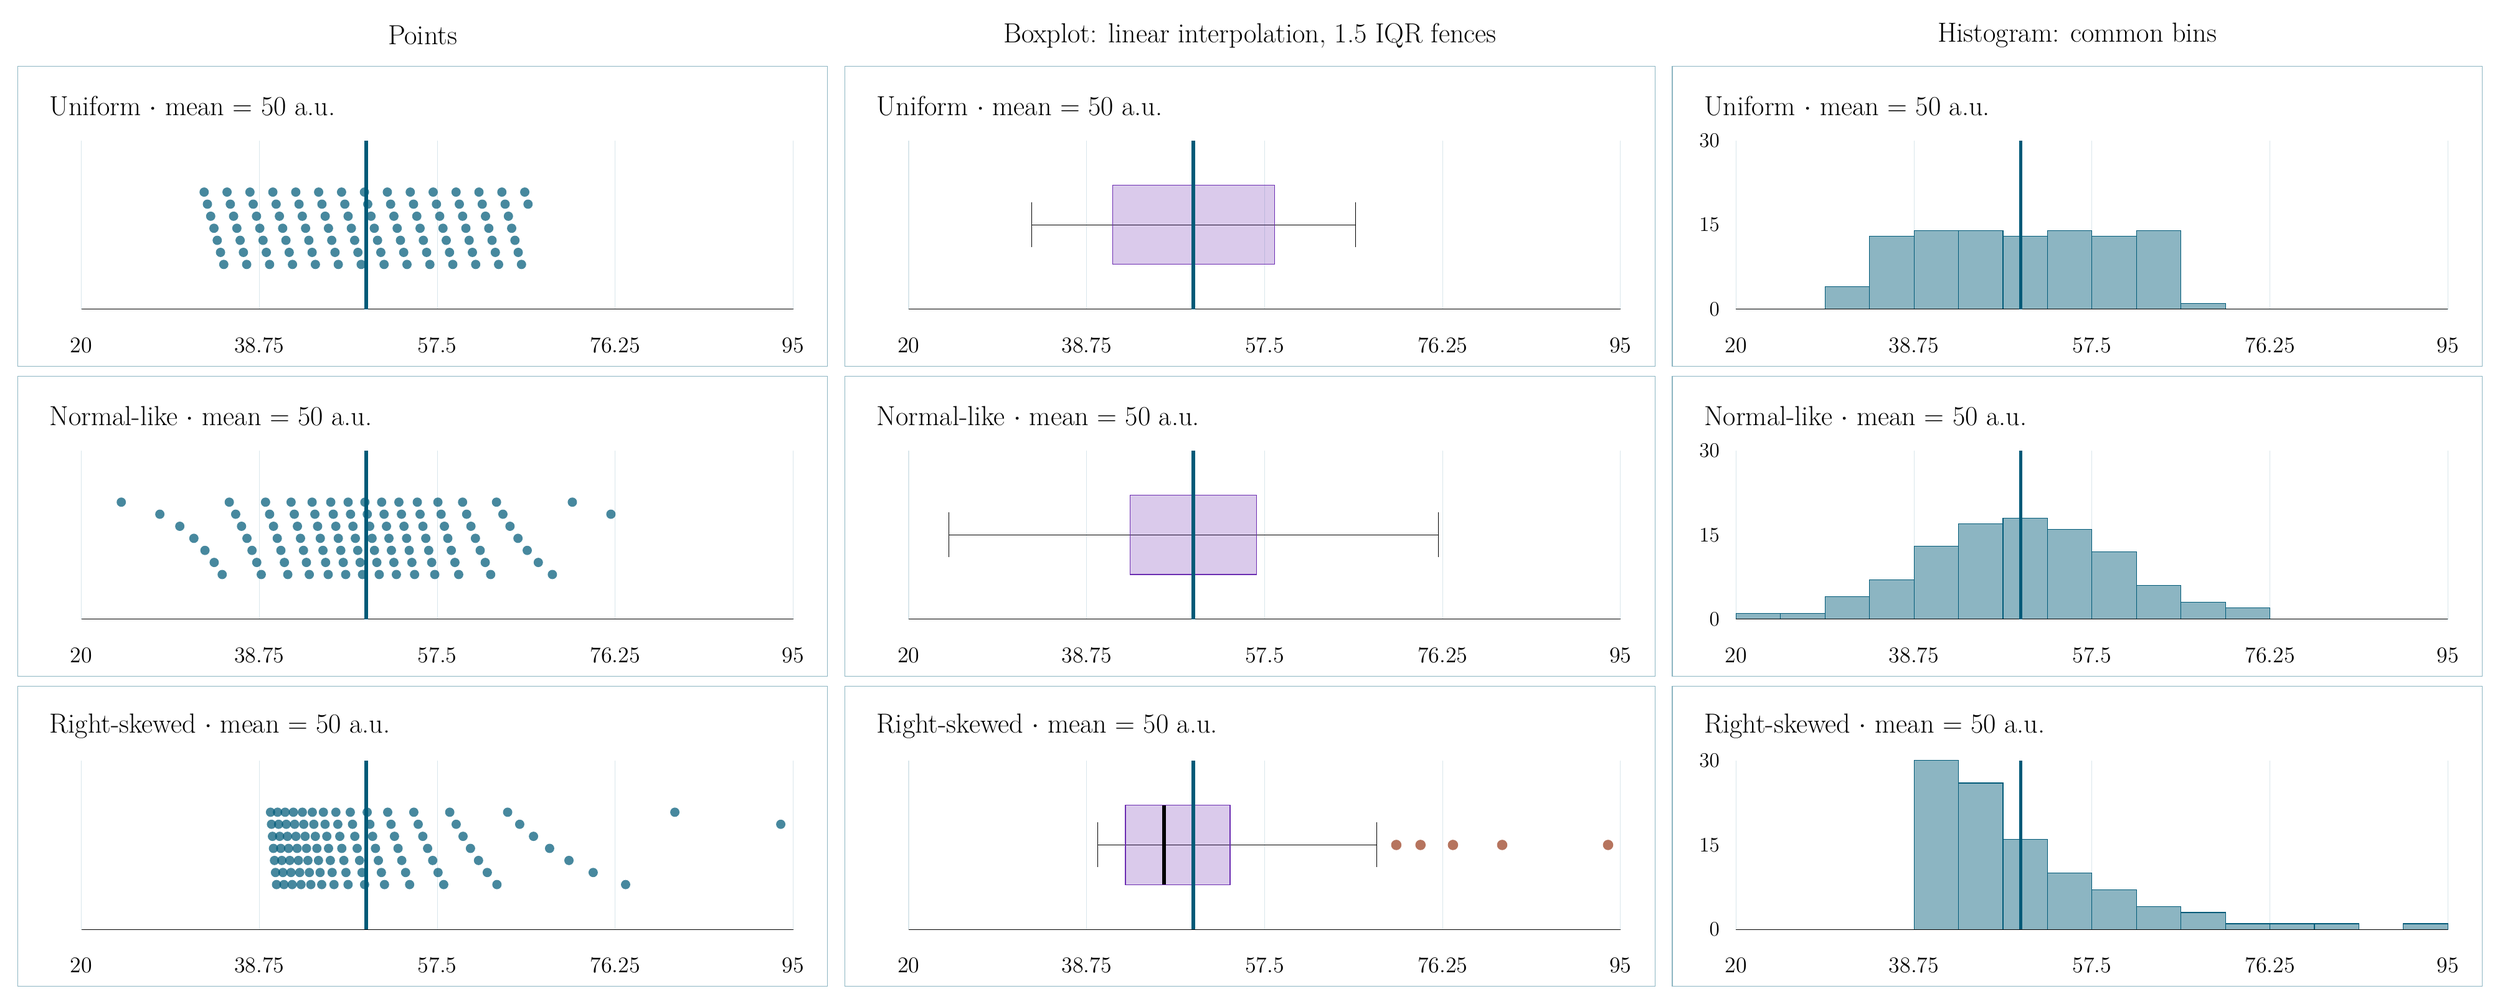
\begin{tikzpicture}[x=1pt,y=-1pt]
\node[anchor=center,font=\fontsize{16}{19}\selectfont] at (240,24) {Points};
\node[anchor=center,font=\fontsize{16}{19}\selectfont] at (720,24) {Boxplot: linear interpolation, 1.5 IQR fences};
\node[anchor=center,font=\fontsize{16}{19}\selectfont] at (1200,24) {Histogram: common bins};
\begin{scope}[shift={(0,40)}]
\path[draw=pcd1!45] (5,2) rectangle (475,176);
\node[anchor=west,font=\fontsize{16}{19}\selectfont] at (20,25) {Uniform \ensuremath{\cdot} mean = 50 a.u.};
\draw[draw=pcd1!15] (42,45) -- (42,143);
\node[anchor=center,font=\fontsize{13}{16}\selectfont] at (42,164) {20};
\draw[draw=pcd1!15] (145.25,45) -- (145.25,143);
\node[anchor=center,font=\fontsize{13}{16}\selectfont] at (145.25,164) {38.75};
\draw[draw=pcd1!15] (248.5,45) -- (248.5,143);
\node[anchor=center,font=\fontsize{13}{16}\selectfont] at (248.5,164) {57.5};
\draw[draw=pcd1!15] (351.75,45) -- (351.75,143);
\node[anchor=center,font=\fontsize{13}{16}\selectfont] at (351.75,164) {76.25};
\draw[draw=pcd1!15] (455,45) -- (455,143);
\node[anchor=center,font=\fontsize{13}{16}\selectfont] at (455,164) {95};
\fill[pcd1,opacity=.72] (113.24412891739694,75) circle[radius=2.7pt];
\fill[pcd1,opacity=.72] (115.14222732310145,82) circle[radius=2.7pt];
\fill[pcd1,opacity=.72] (117.04032572881144,89) circle[radius=2.7pt];
\fill[pcd1,opacity=.72] (118.93842413452143,96) circle[radius=2.7pt];
\fill[pcd1,opacity=.72] (120.83652254023141,103) circle[radius=2.7pt];
\fill[pcd1,opacity=.72] (122.7346209459414,110) circle[radius=2.7pt];
\fill[pcd1,opacity=.72] (124.63271935165137,117) circle[radius=2.7pt];
\fill[pcd1,opacity=.72] (126.53081775736136,75) circle[radius=2.7pt];
\fill[pcd1,opacity=.72] (128.42891616306582,82) circle[radius=2.7pt];
\fill[pcd1,opacity=.72] (130.32701456877584,89) circle[radius=2.7pt];
\fill[pcd1,opacity=.72] (132.2251129744858,96) circle[radius=2.7pt];
\fill[pcd1,opacity=.72] (134.1232113801958,103) circle[radius=2.7pt];
\fill[pcd1,opacity=.72] (136.02130978590577,110) circle[radius=2.7pt];
\fill[pcd1,opacity=.72] (137.9194081916158,117) circle[radius=2.7pt];
\fill[pcd1,opacity=.72] (139.81750659732575,75) circle[radius=2.7pt];
\fill[pcd1,opacity=.72] (141.71560500303025,82) circle[radius=2.7pt];
\fill[pcd1,opacity=.72] (143.61370340874024,89) circle[radius=2.7pt];
\fill[pcd1,opacity=.72] (145.51180181445022,96) circle[radius=2.7pt];
\fill[pcd1,opacity=.72] (147.4099002201602,103) circle[radius=2.7pt];
\fill[pcd1,opacity=.72] (149.3079986258702,110) circle[radius=2.7pt];
\fill[pcd1,opacity=.72] (151.20609703158019,117) circle[radius=2.7pt];
\fill[pcd1,opacity=.72] (153.10419543729017,75) circle[radius=2.7pt];
\fill[pcd1,opacity=.72] (155.00229384299465,82) circle[radius=2.7pt];
\fill[pcd1,opacity=.72] (156.90039224870463,89) circle[radius=2.7pt];
\fill[pcd1,opacity=.72] (158.79849065441462,96) circle[radius=2.7pt];
\fill[pcd1,opacity=.72] (160.6965890601246,103) circle[radius=2.7pt];
\fill[pcd1,opacity=.72] (162.59468746583457,110) circle[radius=2.7pt];
\fill[pcd1,opacity=.72] (164.49278587154458,117) circle[radius=2.7pt];
\fill[pcd1,opacity=.72] (166.39088427725454,75) circle[radius=2.7pt];
\fill[pcd1,opacity=.72] (168.28898268295902,82) circle[radius=2.7pt];
\fill[pcd1,opacity=.72] (170.18708108866903,89) circle[radius=2.7pt];
\fill[pcd1,opacity=.72] (172.085179494379,96) circle[radius=2.7pt];
\fill[pcd1,opacity=.72] (173.98327790008898,103) circle[radius=2.7pt];
\fill[pcd1,opacity=.72] (175.88137630579897,110) circle[radius=2.7pt];
\fill[pcd1,opacity=.72] (177.77947471150895,117) circle[radius=2.7pt];
\fill[pcd1,opacity=.72] (179.67757311721897,75) circle[radius=2.7pt];
\fill[pcd1,opacity=.72] (181.57567152292344,82) circle[radius=2.7pt];
\fill[pcd1,opacity=.72] (183.47376992863343,89) circle[radius=2.7pt];
\fill[pcd1,opacity=.72] (185.37186833434342,96) circle[radius=2.7pt];
\fill[pcd1,opacity=.72] (187.2699667400534,103) circle[radius=2.7pt];
\fill[pcd1,opacity=.72] (189.1680651457634,110) circle[radius=2.7pt];
\fill[pcd1,opacity=.72] (191.06616355147338,117) circle[radius=2.7pt];
\fill[pcd1,opacity=.72] (192.96426195718337,75) circle[radius=2.7pt];
\fill[pcd1,opacity=.72] (194.8623603628878,82) circle[radius=2.7pt];
\fill[pcd1,opacity=.72] (196.76045876859783,89) circle[radius=2.7pt];
\fill[pcd1,opacity=.72] (198.65855717430782,96) circle[radius=2.7pt];
\fill[pcd1,opacity=.72] (200.55665558001778,103) circle[radius=2.7pt];
\fill[pcd1,opacity=.72] (202.4547539857278,110) circle[radius=2.7pt];
\fill[pcd1,opacity=.72] (204.35285239143775,117) circle[radius=2.7pt];
\fill[pcd1,opacity=.72] (206.25095079714774,75) circle[radius=2.7pt];
\fill[pcd1,opacity=.72] (208.14904920285224,82) circle[radius=2.7pt];
\fill[pcd1,opacity=.72] (210.04714760856223,89) circle[radius=2.7pt];
\fill[pcd1,opacity=.72] (211.94524601427224,96) circle[radius=2.7pt];
\fill[pcd1,opacity=.72] (213.8433444199822,103) circle[radius=2.7pt];
\fill[pcd1,opacity=.72] (215.74144282569222,110) circle[radius=2.7pt];
\fill[pcd1,opacity=.72] (217.63954123140218,117) circle[radius=2.7pt];
\fill[pcd1,opacity=.72] (219.53763963711216,75) circle[radius=2.7pt];
\fill[pcd1,opacity=.72] (221.43573804281664,82) circle[radius=2.7pt];
\fill[pcd1,opacity=.72] (223.33383644852663,89) circle[radius=2.7pt];
\fill[pcd1,opacity=.72] (225.2319348542366,96) circle[radius=2.7pt];
\fill[pcd1,opacity=.72] (227.13003325994657,103) circle[radius=2.7pt];
\fill[pcd1,opacity=.72] (229.0281316656566,110) circle[radius=2.7pt];
\fill[pcd1,opacity=.72] (230.92623007136655,117) circle[radius=2.7pt];
\fill[pcd1,opacity=.72] (232.82432847707656,75) circle[radius=2.7pt];
\fill[pcd1,opacity=.72] (234.722426882781,82) circle[radius=2.7pt];
\fill[pcd1,opacity=.72] (236.62052528849105,89) circle[radius=2.7pt];
\fill[pcd1,opacity=.72] (238.51862369420104,96) circle[radius=2.7pt];
\fill[pcd1,opacity=.72] (240.416722099911,103) circle[radius=2.7pt];
\fill[pcd1,opacity=.72] (242.31482050562101,110) circle[radius=2.7pt];
\fill[pcd1,opacity=.72] (244.21291891133097,117) circle[radius=2.7pt];
\fill[pcd1,opacity=.72] (246.11101731704096,75) circle[radius=2.7pt];
\fill[pcd1,opacity=.72] (248.00911572274543,82) circle[radius=2.7pt];
\fill[pcd1,opacity=.72] (249.90721412845545,89) circle[radius=2.7pt];
\fill[pcd1,opacity=.72] (251.8053125341654,96) circle[radius=2.7pt];
\fill[pcd1,opacity=.72] (253.7034109398754,103) circle[radius=2.7pt];
\fill[pcd1,opacity=.72] (255.6015093455854,110) circle[radius=2.7pt];
\fill[pcd1,opacity=.72] (257.49960775129534,117) circle[radius=2.7pt];
\fill[pcd1,opacity=.72] (259.39770615700536,75) circle[radius=2.7pt];
\fill[pcd1,opacity=.72] (261.2958045627098,82) circle[radius=2.7pt];
\fill[pcd1,opacity=.72] (263.1939029684198,89) circle[radius=2.7pt];
\fill[pcd1,opacity=.72] (265.09200137412984,96) circle[radius=2.7pt];
\fill[pcd1,opacity=.72] (266.9900997798398,103) circle[radius=2.7pt];
\fill[pcd1,opacity=.72] (268.88819818554975,110) circle[radius=2.7pt];
\fill[pcd1,opacity=.72] (270.78629659125977,117) circle[radius=2.7pt];
\fill[pcd1,opacity=.72] (272.6843949969698,75) circle[radius=2.7pt];
\fill[pcd1,opacity=.72] (274.58249340267423,82) circle[radius=2.7pt];
\fill[pcd1,opacity=.72] (276.48059180838425,89) circle[radius=2.7pt];
\fill[pcd1,opacity=.72] (278.3786902140942,96) circle[radius=2.7pt];
\fill[pcd1,opacity=.72] (280.27678861980417,103) circle[radius=2.7pt];
\fill[pcd1,opacity=.72] (282.1748870255142,110) circle[radius=2.7pt];
\fill[pcd1,opacity=.72] (284.0729854312242,117) circle[radius=2.7pt];
\fill[pcd1,opacity=.72] (285.97108383693416,75) circle[radius=2.7pt];
\fill[pcd1,opacity=.72] (287.86918224263866,82) circle[radius=2.7pt];
\fill[pcd1,opacity=.72] (289.7672806483487,89) circle[radius=2.7pt];
\fill[pcd1,opacity=.72] (291.6653790540587,96) circle[radius=2.7pt];
\fill[pcd1,opacity=.72] (293.5634774597686,103) circle[radius=2.7pt];
\fill[pcd1,opacity=.72] (295.4615758654786,110) circle[radius=2.7pt];
\fill[pcd1,opacity=.72] (297.3596742711886,117) circle[radius=2.7pt];
\fill[pcd1,opacity=.72] (299.25777267689307,75) circle[radius=2.7pt];
\fill[pcd1,opacity=.72] (301.155871082603,82) circle[radius=2.7pt];
\draw[draw=black] (42,143) -- (455,143);
\draw[draw=pcd1,line width=2pt] (207.19999999999996,45) -- (207.19999999999996,143);
\end{scope}
\begin{scope}[shift={(480,40)}]
\path[draw=pcd1!45] (5,2) rectangle (475,176);
\node[anchor=west,font=\fontsize{16}{19}\selectfont] at (20,25) {Uniform \ensuremath{\cdot} mean = 50 a.u.};
\draw[draw=pcd1!15] (42,45) -- (42,143);
\node[anchor=center,font=\fontsize{13}{16}\selectfont] at (42,164) {20};
\draw[draw=pcd1!15] (145.25,45) -- (145.25,143);
\node[anchor=center,font=\fontsize{13}{16}\selectfont] at (145.25,164) {38.75};
\draw[draw=pcd1!15] (248.5,45) -- (248.5,143);
\node[anchor=center,font=\fontsize{13}{16}\selectfont] at (248.5,164) {57.5};
\draw[draw=pcd1!15] (351.75,45) -- (351.75,143);
\node[anchor=center,font=\fontsize{13}{16}\selectfont] at (351.75,164) {76.25};
\draw[draw=pcd1!15] (455,45) -- (455,143);
\node[anchor=center,font=\fontsize{13}{16}\selectfont] at (455,164) {95};
\draw[draw=black] (113.24412891739694,94) -- (301.155871082603,94);
\path[fill=pcd2,fill opacity=.25,draw=pcd2] (160.22206445869708,71) rectangle (254.1779355413029,117);
\draw[draw=black,line width=2pt] (207.20000000000002,71) -- (207.20000000000002,117);
\draw[draw=black] (113.24412891739694,81) -- (113.24412891739694,107);
\draw[draw=black] (301.155871082603,81) -- (301.155871082603,107);
\draw[draw=black] (42,143) -- (455,143);
\draw[draw=pcd1,line width=2pt] (207.19999999999996,45) -- (207.19999999999996,143);
\end{scope}
\begin{scope}[shift={(960,40)}]
\path[draw=pcd1!45] (5,2) rectangle (475,176);
\node[anchor=west,font=\fontsize{16}{19}\selectfont] at (20,25) {Uniform \ensuremath{\cdot} mean = 50 a.u.};
\draw[draw=pcd1!15] (42,45) -- (42,143);
\node[anchor=center,font=\fontsize{13}{16}\selectfont] at (42,164) {20};
\draw[draw=pcd1!15] (145.25,45) -- (145.25,143);
\node[anchor=center,font=\fontsize{13}{16}\selectfont] at (145.25,164) {38.75};
\draw[draw=pcd1!15] (248.5,45) -- (248.5,143);
\node[anchor=center,font=\fontsize{13}{16}\selectfont] at (248.5,164) {57.5};
\draw[draw=pcd1!15] (351.75,45) -- (351.75,143);
\node[anchor=center,font=\fontsize{13}{16}\selectfont] at (351.75,164) {76.25};
\draw[draw=pcd1!15] (455,45) -- (455,143);
\node[anchor=center,font=\fontsize{13}{16}\selectfont] at (455,164) {95};
\path[fill=pcd1,fill opacity=.45,draw=pcd1] (42,143) rectangle (67.8125,143);
\path[fill=pcd1,fill opacity=.45,draw=pcd1] (67.8125,143) rectangle (93.625,143);
\path[fill=pcd1,fill opacity=.45,draw=pcd1] (93.625,129.93333333333334) rectangle (119.4375,143);
\path[fill=pcd1,fill opacity=.45,draw=pcd1] (119.4375,100.53333333333333) rectangle (145.25,143);
\path[fill=pcd1,fill opacity=.45,draw=pcd1] (145.25,97.26666666666667) rectangle (171.0625,143);
\path[fill=pcd1,fill opacity=.45,draw=pcd1] (171.0625,97.26666666666667) rectangle (196.875,143);
\path[fill=pcd1,fill opacity=.45,draw=pcd1] (196.875,100.53333333333333) rectangle (222.6875,143);
\path[fill=pcd1,fill opacity=.45,draw=pcd1] (222.6875,97.26666666666667) rectangle (248.5,143);
\path[fill=pcd1,fill opacity=.45,draw=pcd1] (248.5,100.53333333333333) rectangle (274.3125,143);
\path[fill=pcd1,fill opacity=.45,draw=pcd1] (274.3125,97.26666666666667) rectangle (300.125,143);
\path[fill=pcd1,fill opacity=.45,draw=pcd1] (300.125,139.73333333333332) rectangle (325.9375,143);
\path[fill=pcd1,fill opacity=.45,draw=pcd1] (325.9375,143) rectangle (351.75,143);
\path[fill=pcd1,fill opacity=.45,draw=pcd1] (351.75,143) rectangle (377.5625,143);
\path[fill=pcd1,fill opacity=.45,draw=pcd1] (377.5625,143) rectangle (403.375,143);
\path[fill=pcd1,fill opacity=.45,draw=pcd1] (403.375,143) rectangle (429.1875,143);
\path[fill=pcd1,fill opacity=.45,draw=pcd1] (429.1875,143) rectangle (455,143);
\node[anchor=east,font=\fontsize{12}{15}\selectfont] at (36,143) {0};
\node[anchor=east,font=\fontsize{12}{15}\selectfont] at (36,94) {15};
\node[anchor=east,font=\fontsize{12}{15}\selectfont] at (36,45) {30};
\draw[draw=black] (42,143) -- (455,143);
\draw[draw=pcd1,line width=2pt] (207.19999999999996,45) -- (207.19999999999996,143);
\end{scope}
\begin{scope}[shift={(0,220)}]
\path[draw=pcd1!45] (5,2) rectangle (475,176);
\node[anchor=west,font=\fontsize{16}{19}\selectfont] at (20,25) {Normal-like \ensuremath{\cdot} mean = 50 a.u.};
\draw[draw=pcd1!15] (42,45) -- (42,143);
\node[anchor=center,font=\fontsize{13}{16}\selectfont] at (42,164) {20};
\draw[draw=pcd1!15] (145.25,45) -- (145.25,143);
\node[anchor=center,font=\fontsize{13}{16}\selectfont] at (145.25,164) {38.75};
\draw[draw=pcd1!15] (248.5,45) -- (248.5,143);
\node[anchor=center,font=\fontsize{13}{16}\selectfont] at (248.5,164) {57.5};
\draw[draw=pcd1!15] (351.75,45) -- (351.75,143);
\node[anchor=center,font=\fontsize{13}{16}\selectfont] at (351.75,164) {76.25};
\draw[draw=pcd1!15] (455,45) -- (455,143);
\node[anchor=center,font=\fontsize{13}{16}\selectfont] at (455,164) {95};
\fill[pcd1,opacity=.72] (65.16454133626237,75) circle[radius=2.7pt];
\fill[pcd1,opacity=.72] (87.53765215058463,82) circle[radius=2.7pt];
\fill[pcd1,opacity=.72] (99.12436660107437,89) circle[radius=2.7pt];
\fill[pcd1,opacity=.72] (107.28826938338861,96) circle[radius=2.7pt];
\fill[pcd1,opacity=.72] (113.7129855211349,103) circle[radius=2.7pt];
\fill[pcd1,opacity=.72] (119.0730051912103,110) circle[radius=2.7pt];
\fill[pcd1,opacity=.72] (123.70993496528129,117) circle[radius=2.7pt];
\fill[pcd1,opacity=.72] (127.82187022489454,75) circle[radius=2.7pt];
\fill[pcd1,opacity=.72] (131.53442809166978,82) circle[radius=2.7pt];
\fill[pcd1,opacity=.72] (134.93251509506104,89) circle[radius=2.7pt];
\fill[pcd1,opacity=.72] (138.07634270918393,96) circle[radius=2.7pt];
\fill[pcd1,opacity=.72] (141.01024094780104,103) circle[radius=2.7pt];
\fill[pcd1,opacity=.72] (143.76784568754908,110) circle[radius=2.7pt];
\fill[pcd1,opacity=.72] (146.37531884246346,117) circle[radius=2.7pt];
\fill[pcd1,opacity=.72] (148.85343600881788,75) circle[radius=2.7pt];
\fill[pcd1,opacity=.72] (151.21898956004614,82) circle[radius=2.7pt];
\fill[pcd1,opacity=.72] (153.48576081178732,89) circle[radius=2.7pt];
\fill[pcd1,opacity=.72] (155.66521140319736,96) circle[radius=2.7pt];
\fill[pcd1,opacity=.72] (157.7669862283159,103) circle[radius=2.7pt];
\fill[pcd1,opacity=.72] (159.7992865920125,110) circle[radius=2.7pt];
\fill[pcd1,opacity=.72] (161.76915195659856,117) circle[radius=2.7pt];
\fill[pcd1,opacity=.72] (163.68267600478754,75) circle[radius=2.7pt];
\fill[pcd1,opacity=.72] (165.54517465782482,82) circle[radius=2.7pt];
\fill[pcd1,opacity=.72] (167.36131838621117,89) circle[radius=2.7pt];
\fill[pcd1,opacity=.72] (169.1352375982878,96) circle[radius=2.7pt];
\fill[pcd1,opacity=.72] (170.87060746462737,103) circle[radius=2.7pt];
\fill[pcd1,opacity=.72] (172.5707168478382,110) circle[radius=2.7pt];
\fill[pcd1,opacity=.72] (174.2385248135968,117) circle[radius=2.7pt];
\fill[pcd1,opacity=.72] (175.87670734235186,75) circle[radius=2.7pt];
\fill[pcd1,opacity=.72] (177.4876962383739,82) circle[radius=2.7pt];
\fill[pcd1,opacity=.72] (179.07371177394688,89) circle[radius=2.7pt];
\fill[pcd1,opacity=.72] (180.63679026512506,96) circle[radius=2.7pt];
\fill[pcd1,opacity=.72] (182.17880751793538,103) circle[radius=2.7pt];
\fill[pcd1,opacity=.72] (183.7014988885424,110) circle[radius=2.7pt];
\fill[pcd1,opacity=.72] (185.20647655075038,117) circle[radius=2.7pt];
\fill[pcd1,opacity=.72] (186.69524444809016,75) circle[radius=2.7pt];
\fill[pcd1,opacity=.72] (188.16921131713553,82) circle[radius=2.7pt];
\fill[pcd1,opacity=.72] (189.62970209763023,89) circle[radius=2.7pt];
\fill[pcd1,opacity=.72] (191.07796798874614,96) circle[radius=2.7pt];
\fill[pcd1,opacity=.72] (192.51519536587472,103) circle[radius=2.7pt];
\fill[pcd1,opacity=.72] (193.94251373685682,110) circle[radius=2.7pt];
\fill[pcd1,opacity=.72] (195.36100288752172,117) circle[radius=2.7pt];
\fill[pcd1,opacity=.72] (196.77169934342442,75) circle[radius=2.7pt];
\fill[pcd1,opacity=.72] (198.17560225582272,82) circle[radius=2.7pt];
\fill[pcd1,opacity=.72] (199.57367880477972,89) circle[radius=2.7pt];
\fill[pcd1,opacity=.72] (200.96686920014255,96) circle[radius=2.7pt];
\fill[pcd1,opacity=.72] (202.3560913510083,103) circle[radius=2.7pt];
\fill[pcd1,opacity=.72] (203.74224526671262,110) circle[radius=2.7pt];
\fill[pcd1,opacity=.72] (205.1262172457786,117) circle[radius=2.7pt];
\fill[pcd1,opacity=.72] (206.50888390477604,75) circle[radius=2.7pt];
\fill[pcd1,opacity=.72] (207.89111609522396,82) circle[radius=2.7pt];
\fill[pcd1,opacity=.72] (209.27378275422137,89) circle[radius=2.7pt];
\fill[pcd1,opacity=.72] (210.6577547332874,96) circle[radius=2.7pt];
\fill[pcd1,opacity=.72] (212.0439086489917,103) circle[radius=2.7pt];
\fill[pcd1,opacity=.72] (213.43313079985745,110) circle[radius=2.7pt];
\fill[pcd1,opacity=.72] (214.8263211952203,117) circle[radius=2.7pt];
\fill[pcd1,opacity=.72] (216.22439774417728,75) circle[radius=2.7pt];
\fill[pcd1,opacity=.72] (217.62830065657556,82) circle[radius=2.7pt];
\fill[pcd1,opacity=.72] (219.03899711247826,89) circle[radius=2.7pt];
\fill[pcd1,opacity=.72] (220.45748626314318,96) circle[radius=2.7pt];
\fill[pcd1,opacity=.72] (221.8848046341253,103) circle[radius=2.7pt];
\fill[pcd1,opacity=.72] (223.32203201125384,110) circle[radius=2.7pt];
\fill[pcd1,opacity=.72] (224.77029790236978,117) circle[radius=2.7pt];
\fill[pcd1,opacity=.72] (226.23078868286447,75) circle[radius=2.7pt];
\fill[pcd1,opacity=.72] (227.70475555190984,82) circle[radius=2.7pt];
\fill[pcd1,opacity=.72] (229.1935234492496,89) circle[radius=2.7pt];
\fill[pcd1,opacity=.72] (230.6985011114576,96) circle[radius=2.7pt];
\fill[pcd1,opacity=.72] (232.22119248206462,103) circle[radius=2.7pt];
\fill[pcd1,opacity=.72] (233.76320973487495,110) circle[radius=2.7pt];
\fill[pcd1,opacity=.72] (235.3262882260531,117) circle[radius=2.7pt];
\fill[pcd1,opacity=.72] (236.91230376162608,75) circle[radius=2.7pt];
\fill[pcd1,opacity=.72] (238.52329265764814,82) circle[radius=2.7pt];
\fill[pcd1,opacity=.72] (240.16147518640324,89) circle[radius=2.7pt];
\fill[pcd1,opacity=.72] (241.8292831521618,96) circle[radius=2.7pt];
\fill[pcd1,opacity=.72] (243.52939253537264,103) circle[radius=2.7pt];
\fill[pcd1,opacity=.72] (245.2647624017122,110) circle[radius=2.7pt];
\fill[pcd1,opacity=.72] (247.03868161378887,117) circle[radius=2.7pt];
\fill[pcd1,opacity=.72] (248.8548253421752,75) circle[radius=2.7pt];
\fill[pcd1,opacity=.72] (250.71732399521247,82) circle[radius=2.7pt];
\fill[pcd1,opacity=.72] (252.63084804340141,89) circle[radius=2.7pt];
\fill[pcd1,opacity=.72] (254.60071340798754,96) circle[radius=2.7pt];
\fill[pcd1,opacity=.72] (256.6330137716841,103) circle[radius=2.7pt];
\fill[pcd1,opacity=.72] (258.7347885968027,110) circle[radius=2.7pt];
\fill[pcd1,opacity=.72] (260.9142391882127,117) circle[radius=2.7pt];
\fill[pcd1,opacity=.72] (263.18101043995387,75) circle[radius=2.7pt];
\fill[pcd1,opacity=.72] (265.5465639911821,82) circle[radius=2.7pt];
\fill[pcd1,opacity=.72] (268.0246811575365,89) circle[radius=2.7pt];
\fill[pcd1,opacity=.72] (270.63215431245095,96) circle[radius=2.7pt];
\fill[pcd1,opacity=.72] (273.389759052199,103) circle[radius=2.7pt];
\fill[pcd1,opacity=.72] (276.3236572908161,110) circle[radius=2.7pt];
\fill[pcd1,opacity=.72] (279.46748490493894,117) circle[radius=2.7pt];
\fill[pcd1,opacity=.72] (282.86557190833025,75) circle[radius=2.7pt];
\fill[pcd1,opacity=.72] (286.5781297751055,82) circle[radius=2.7pt];
\fill[pcd1,opacity=.72] (290.6900650347187,89) circle[radius=2.7pt];
\fill[pcd1,opacity=.72] (295.3269948087898,96) circle[radius=2.7pt];
\fill[pcd1,opacity=.72] (300.6870144788651,103) circle[radius=2.7pt];
\fill[pcd1,opacity=.72] (307.1117306166114,110) circle[radius=2.7pt];
\fill[pcd1,opacity=.72] (315.27563339892566,117) circle[radius=2.7pt];
\fill[pcd1,opacity=.72] (326.86234784941536,75) circle[radius=2.7pt];
\fill[pcd1,opacity=.72] (349.2354586637376,82) circle[radius=2.7pt];
\draw[draw=black] (42,143) -- (455,143);
\draw[draw=pcd1,line width=2pt] (207.20000000000002,45) -- (207.20000000000002,143);
\end{scope}
\begin{scope}[shift={(480,220)}]
\path[draw=pcd1!45] (5,2) rectangle (475,176);
\node[anchor=west,font=\fontsize{16}{19}\selectfont] at (20,25) {Normal-like \ensuremath{\cdot} mean = 50 a.u.};
\draw[draw=pcd1!15] (42,45) -- (42,143);
\node[anchor=center,font=\fontsize{13}{16}\selectfont] at (42,164) {20};
\draw[draw=pcd1!15] (145.25,45) -- (145.25,143);
\node[anchor=center,font=\fontsize{13}{16}\selectfont] at (145.25,164) {38.75};
\draw[draw=pcd1!15] (248.5,45) -- (248.5,143);
\node[anchor=center,font=\fontsize{13}{16}\selectfont] at (248.5,164) {57.5};
\draw[draw=pcd1!15] (351.75,45) -- (351.75,143);
\node[anchor=center,font=\fontsize{13}{16}\selectfont] at (351.75,164) {76.25};
\draw[draw=pcd1!15] (455,45) -- (455,143);
\node[anchor=center,font=\fontsize{13}{16}\selectfont] at (455,164) {95};
\draw[draw=black] (65.16454133626237,94) -- (349.2354586637376,94);
\path[fill=pcd2,fill opacity=.25,draw=pcd2] (170.43676499804246,71) rectangle (243.96323500195754,117);
\draw[draw=black,line width=2pt] (207.20000000000002,71) -- (207.20000000000002,117);
\draw[draw=black] (65.16454133626237,81) -- (65.16454133626237,107);
\draw[draw=black] (349.2354586637376,81) -- (349.2354586637376,107);
\draw[draw=black] (42,143) -- (455,143);
\draw[draw=pcd1,line width=2pt] (207.20000000000002,45) -- (207.20000000000002,143);
\end{scope}
\begin{scope}[shift={(960,220)}]
\path[draw=pcd1!45] (5,2) rectangle (475,176);
\node[anchor=west,font=\fontsize{16}{19}\selectfont] at (20,25) {Normal-like \ensuremath{\cdot} mean = 50 a.u.};
\draw[draw=pcd1!15] (42,45) -- (42,143);
\node[anchor=center,font=\fontsize{13}{16}\selectfont] at (42,164) {20};
\draw[draw=pcd1!15] (145.25,45) -- (145.25,143);
\node[anchor=center,font=\fontsize{13}{16}\selectfont] at (145.25,164) {38.75};
\draw[draw=pcd1!15] (248.5,45) -- (248.5,143);
\node[anchor=center,font=\fontsize{13}{16}\selectfont] at (248.5,164) {57.5};
\draw[draw=pcd1!15] (351.75,45) -- (351.75,143);
\node[anchor=center,font=\fontsize{13}{16}\selectfont] at (351.75,164) {76.25};
\draw[draw=pcd1!15] (455,45) -- (455,143);
\node[anchor=center,font=\fontsize{13}{16}\selectfont] at (455,164) {95};
\path[fill=pcd1,fill opacity=.45,draw=pcd1] (42,139.73333333333332) rectangle (67.8125,143);
\path[fill=pcd1,fill opacity=.45,draw=pcd1] (67.8125,139.73333333333332) rectangle (93.625,143);
\path[fill=pcd1,fill opacity=.45,draw=pcd1] (93.625,129.93333333333334) rectangle (119.4375,143);
\path[fill=pcd1,fill opacity=.45,draw=pcd1] (119.4375,120.13333333333333) rectangle (145.25,143);
\path[fill=pcd1,fill opacity=.45,draw=pcd1] (145.25,100.53333333333333) rectangle (171.0625,143);
\path[fill=pcd1,fill opacity=.45,draw=pcd1] (171.0625,87.46666666666667) rectangle (196.875,143);
\path[fill=pcd1,fill opacity=.45,draw=pcd1] (196.875,84.2) rectangle (222.6875,143);
\path[fill=pcd1,fill opacity=.45,draw=pcd1] (222.6875,90.73333333333333) rectangle (248.5,143);
\path[fill=pcd1,fill opacity=.45,draw=pcd1] (248.5,103.8) rectangle (274.3125,143);
\path[fill=pcd1,fill opacity=.45,draw=pcd1] (274.3125,123.4) rectangle (300.125,143);
\path[fill=pcd1,fill opacity=.45,draw=pcd1] (300.125,133.2) rectangle (325.9375,143);
\path[fill=pcd1,fill opacity=.45,draw=pcd1] (325.9375,136.46666666666667) rectangle (351.75,143);
\path[fill=pcd1,fill opacity=.45,draw=pcd1] (351.75,143) rectangle (377.5625,143);
\path[fill=pcd1,fill opacity=.45,draw=pcd1] (377.5625,143) rectangle (403.375,143);
\path[fill=pcd1,fill opacity=.45,draw=pcd1] (403.375,143) rectangle (429.1875,143);
\path[fill=pcd1,fill opacity=.45,draw=pcd1] (429.1875,143) rectangle (455,143);
\node[anchor=east,font=\fontsize{12}{15}\selectfont] at (36,143) {0};
\node[anchor=east,font=\fontsize{12}{15}\selectfont] at (36,94) {15};
\node[anchor=east,font=\fontsize{12}{15}\selectfont] at (36,45) {30};
\draw[draw=black] (42,143) -- (455,143);
\draw[draw=pcd1,line width=2pt] (207.20000000000002,45) -- (207.20000000000002,143);
\end{scope}
\begin{scope}[shift={(0,400)}]
\path[draw=pcd1!45] (5,2) rectangle (475,176);
\node[anchor=west,font=\fontsize{16}{19}\selectfont] at (20,25) {Right-skewed \ensuremath{\cdot} mean = 50 a.u.};
\draw[draw=pcd1!15] (42,45) -- (42,143);
\node[anchor=center,font=\fontsize{13}{16}\selectfont] at (42,164) {20};
\draw[draw=pcd1!15] (145.25,45) -- (145.25,143);
\node[anchor=center,font=\fontsize{13}{16}\selectfont] at (145.25,164) {38.75};
\draw[draw=pcd1!15] (248.5,45) -- (248.5,143);
\node[anchor=center,font=\fontsize{13}{16}\selectfont] at (248.5,164) {57.5};
\draw[draw=pcd1!15] (351.75,45) -- (351.75,143);
\node[anchor=center,font=\fontsize{13}{16}\selectfont] at (351.75,164) {76.25};
\draw[draw=pcd1!15] (455,45) -- (455,143);
\node[anchor=center,font=\fontsize{13}{16}\selectfont] at (455,164) {95};
\fill[pcd1,opacity=.72] (151.74905333266133,75) circle[radius=2.7pt];
\fill[pcd1,opacity=.72] (152.31395571301317,82) circle[radius=2.7pt];
\fill[pcd1,opacity=.72] (152.8846225028966,89) circle[radius=2.7pt];
\fill[pcd1,opacity=.72] (153.4611725592456,96) circle[radius=2.7pt];
\fill[pcd1,opacity=.72] (154.04372845340623,103) circle[radius=2.7pt];
\fill[pcd1,opacity=.72] (154.63241662752557,110) circle[radius=2.7pt];
\fill[pcd1,opacity=.72] (155.22736755930603,117) circle[radius=2.7pt];
\fill[pcd1,opacity=.72] (155.8287159355586,75) circle[radius=2.7pt];
\fill[pcd1,opacity=.72] (156.4366008352228,82) circle[radius=2.7pt];
\fill[pcd1,opacity=.72] (157.0511659224521,89) circle[radius=2.7pt];
\fill[pcd1,opacity=.72] (157.67255965038294,96) circle[radius=2.7pt];
\fill[pcd1,opacity=.72] (158.3009354764065,103) circle[radius=2.7pt];
\fill[pcd1,opacity=.72] (158.93645208964392,110) circle[radius=2.7pt];
\fill[pcd1,opacity=.72] (159.5792736514773,117) circle[radius=2.7pt];
\fill[pcd1,opacity=.72] (160.22957005010642,75) circle[radius=2.7pt];
\fill[pcd1,opacity=.72] (160.88751717007247,82) circle[radius=2.7pt];
\fill[pcd1,opacity=.72] (161.55329717777346,89) circle[radius=2.7pt];
\fill[pcd1,opacity=.72] (162.22709882426457,96) circle[radius=2.7pt];
\fill[pcd1,opacity=.72] (162.90911776645657,103) circle[radius=2.7pt];
\fill[pcd1,opacity=.72] (163.59955690818776,110) circle[radius=2.7pt];
\fill[pcd1,opacity=.72] (164.2986267625626,117) circle[radius=2.7pt];
\fill[pcd1,opacity=.72] (165.00654583728073,75) circle[radius=2.7pt];
\fill[pcd1,opacity=.72] (165.7235410446304,82) circle[radius=2.7pt];
\fill[pcd1,opacity=.72] (166.44984813813954,89) circle[radius=2.7pt];
\fill[pcd1,opacity=.72] (167.1857121779055,96) circle[radius=2.7pt];
\fill[pcd1,opacity=.72] (167.93138802701577,103) circle[radius=2.7pt];
\fill[pcd1,opacity=.72] (168.68714088144333,110) circle[radius=2.7pt];
\fill[pcd1,opacity=.72] (169.4532468363193,117) circle[radius=2.7pt];
\fill[pcd1,opacity=.72] (170.229993491435,75) circle[radius=2.7pt];
\fill[pcd1,opacity=.72] (171.01768059949208,82) circle[radius=2.7pt];
\fill[pcd1,opacity=.72] (171.8166207605925,89) circle[radius=2.7pt];
\fill[pcd1,opacity=.72] (172.6271401670594,96) circle[radius=2.7pt];
\fill[pcd1,opacity=.72] (173.44957940309263,103) circle[radius=2.7pt];
\fill[pcd1,opacity=.72] (174.28429430402963,110) circle[radius=2.7pt];
\fill[pcd1,opacity=.72] (175.13165688074383,117) circle[radius=2.7pt];
\fill[pcd1,opacity=.72] (175.99205631517825,75) circle[radius=2.7pt];
\fill[pcd1,opacity=.72] (176.86590003362252,82) circle[radius=2.7pt];
\fill[pcd1,opacity=.72] (177.753614865211,89) circle[radius=2.7pt];
\fill[pcd1,opacity=.72] (178.65564829385775,96) circle[radius=2.7pt];
\fill[pcd1,opacity=.72] (179.57246981280298,103) circle[radius=2.7pt];
\fill[pcd1,opacity=.72] (180.5045723920573,110) circle[radius=2.7pt];
\fill[pcd1,opacity=.72] (181.45247407026855,117) circle[radius=2.7pt];
\fill[pcd1,opacity=.72] (182.41671968376033,75) circle[radius=2.7pt];
\fill[pcd1,opacity=.72] (183.39788274731754,82) circle[radius=2.7pt];
\fill[pcd1,opacity=.72] (184.3965675029305,89) circle[radius=2.7pt];
\fill[pcd1,opacity=.72] (185.41341115475836,96) circle[radius=2.7pt];
\fill[pcd1,opacity=.72] (186.44908631115385,103) circle[radius=2.7pt];
\fill[pcd1,opacity=.72] (187.5043036570159,110) circle[radius=2.7pt];
\fill[pcd1,opacity=.72] (188.5798148832203,117) circle[radius=2.7pt];
\fill[pcd1,opacity=.72] (189.6764159032678,75) circle[radius=2.7pt];
\fill[pcd1,opacity=.72] (190.79495039163652,82) circle[radius=2.7pt];
\fill[pcd1,opacity=.72] (191.93631368331717,89) circle[radius=2.7pt];
\fill[pcd1,opacity=.72] (193.10145707959668,96) circle[radius=2.7pt];
\fill[pcd1,opacity=.72] (194.29139261200237,103) circle[radius=2.7pt];
\fill[pcd1,opacity=.72] (195.50719832418628,110) circle[radius=2.7pt];
\fill[pcd1,opacity=.72] (196.75002414084807,117) circle[radius=2.7pt];
\fill[pcd1,opacity=.72] (198.02109840369124,75) circle[radius=2.7pt];
\fill[pcd1,opacity=.72] (199.32173516762984,82) circle[radius=2.7pt];
\fill[pcd1,opacity=.72] (200.65334236577635,89) circle[radius=2.7pt];
\fill[pcd1,opacity=.72] (202.01743097046457,96) circle[radius=2.7pt];
\fill[pcd1,opacity=.72] (203.41562529973626,103) circle[radius=2.7pt];
\fill[pcd1,opacity=.72] (204.8496746455543,110) circle[radius=2.7pt];
\fill[pcd1,opacity=.72] (206.32146643258295,117) circle[radius=2.7pt];
\fill[pcd1,opacity=.72] (207.83304115577005,75) circle[radius=2.7pt];
\fill[pcd1,opacity=.72] (209.38660939333695,82) circle[radius=2.7pt];
\fill[pcd1,opacity=.72] (210.98457125113228,89) circle[radius=2.7pt];
\fill[pcd1,opacity=.72] (212.62953866760014,96) circle[radius=2.7pt];
\fill[pcd1,opacity=.72] (214.32436109975887,103) circle[radius=2.7pt];
\fill[pcd1,opacity=.72] (216.07215522438784,110) circle[radius=2.7pt];
\fill[pcd1,opacity=.72] (217.87633943208505,117) circle[radius=2.7pt];
\fill[pcd1,opacity=.72] (219.74067407326876,75) circle[radius=2.7pt];
\fill[pcd1,opacity=.72] (221.66930864696866,82) circle[radius=2.7pt];
\fill[pcd1,opacity=.72] (223.6668374211214,89) circle[radius=2.7pt];
\fill[pcd1,opacity=.72] (225.73836535942488,96) circle[radius=2.7pt];
\fill[pcd1,opacity=.72] (227.8895867350018,103) circle[radius=2.7pt];
\fill[pcd1,opacity=.72] (230.12687947830563,110) circle[radius=2.7pt];
\fill[pcd1,opacity=.72] (232.45741919635435,117) circle[radius=2.7pt];
\fill[pcd1,opacity=.72] (234.88931799995487,75) circle[radius=2.7pt];
\fill[pcd1,opacity=.72] (237.43179491204052,82) circle[radius=2.7pt];
\fill[pcd1,opacity=.72] (240.09538689072,89) circle[radius=2.7pt];
\fill[pcd1,opacity=.72] (242.89221266713076,96) circle[radius=2.7pt];
\fill[pcd1,opacity=.72] (245.83630609978727,103) circle[radius=2.7pt];
\fill[pcd1,opacity=.72] (248.94404225387817,110) circle[radius=2.7pt];
\fill[pcd1,opacity=.72] (252.23468898849328,117) circle[radius=2.7pt];
\fill[pcd1,opacity=.72] (255.7311312088646,75) circle[radius=2.7pt];
\fill[pcd1,opacity=.72] (259.4608370005535,82) circle[radius=2.7pt];
\fill[pcd1,opacity=.72] (263.4571695673268,89) circle[radius=2.7pt];
\fill[pcd1,opacity=.72] (267.76120502944525,96) circle[radius=2.7pt];
\fill[pcd1,opacity=.72] (272.4243098479891,103) circle[radius=2.7pt];
\fill[pcd1,opacity=.72] (277.51189382125017,110) circle[radius=2.7pt];
\fill[pcd1,opacity=.72] (283.10904724383096,117) circle[radius=2.7pt];
\fill[pcd1,opacity=.72] (289.3293253318585,75) circle[radius=2.7pt];
\fill[pcd1,opacity=.72] (296.32905659681717,82) circle[radius=2.7pt];
\fill[pcd1,opacity=.72] (304.33195126399306,89) circle[radius=2.7pt];
\fill[pcd1,opacity=.72] (313.67442758535555,96) circle[radius=2.7pt];
\fill[pcd1,opacity=.72] (324.89690816418914,103) circle[radius=2.7pt];
\fill[pcd1,opacity=.72] (338.9516324181069,110) circle[radius=2.7pt];
\fill[pcd1,opacity=.72] (357.76879519367947,117) circle[radius=2.7pt];
\fill[pcd1,opacity=.72] (386.3366467610514,75) circle[radius=2.7pt];
\fill[pcd1,opacity=.72] (447.7763853579136,82) circle[radius=2.7pt];
\draw[draw=black] (42,143) -- (455,143);
\draw[draw=pcd1,line width=2pt] (207.19999999999996,45) -- (207.19999999999996,143);
\end{scope}
\begin{scope}[shift={(480,400)}]
\path[draw=pcd1!45] (5,2) rectangle (475,176);
\node[anchor=west,font=\fontsize{16}{19}\selectfont] at (20,25) {Right-skewed \ensuremath{\cdot} mean = 50 a.u.};
\draw[draw=pcd1!15] (42,45) -- (42,143);
\node[anchor=center,font=\fontsize{13}{16}\selectfont] at (42,164) {20};
\draw[draw=pcd1!15] (145.25,45) -- (145.25,143);
\node[anchor=center,font=\fontsize{13}{16}\selectfont] at (145.25,164) {38.75};
\draw[draw=pcd1!15] (248.5,45) -- (248.5,143);
\node[anchor=center,font=\fontsize{13}{16}\selectfont] at (248.5,164) {57.5};
\draw[draw=pcd1!15] (351.75,45) -- (351.75,143);
\node[anchor=center,font=\fontsize{13}{16}\selectfont] at (351.75,164) {76.25};
\draw[draw=pcd1!15] (455,45) -- (455,143);
\node[anchor=center,font=\fontsize{13}{16}\selectfont] at (455,164) {95};
\draw[draw=black] (151.74905333266133,94) -- (313.67442758535555,94);
\path[fill=pcd2,fill opacity=.25,draw=pcd2] (167.7449690647382,71) rectangle (228.4489099208277,117);
\draw[draw=black,line width=2pt] (190.23568314745216,71) -- (190.23568314745216,117);
\draw[draw=black] (151.74905333266133,81) -- (151.74905333266133,107);
\draw[draw=black] (313.67442758535555,81) -- (313.67442758535555,107);
\fill[pcd4,opacity=.72] (324.89690816418914,94) circle[radius=3pt];
\fill[pcd4,opacity=.72] (338.9516324181069,94) circle[radius=3pt];
\fill[pcd4,opacity=.72] (357.76879519367947,94) circle[radius=3pt];
\fill[pcd4,opacity=.72] (386.3366467610514,94) circle[radius=3pt];
\fill[pcd4,opacity=.72] (447.7763853579136,94) circle[radius=3pt];
\draw[draw=black] (42,143) -- (455,143);
\draw[draw=pcd1,line width=2pt] (207.19999999999996,45) -- (207.19999999999996,143);
\end{scope}
\begin{scope}[shift={(960,400)}]
\path[draw=pcd1!45] (5,2) rectangle (475,176);
\node[anchor=west,font=\fontsize{16}{19}\selectfont] at (20,25) {Right-skewed \ensuremath{\cdot} mean = 50 a.u.};
\draw[draw=pcd1!15] (42,45) -- (42,143);
\node[anchor=center,font=\fontsize{13}{16}\selectfont] at (42,164) {20};
\draw[draw=pcd1!15] (145.25,45) -- (145.25,143);
\node[anchor=center,font=\fontsize{13}{16}\selectfont] at (145.25,164) {38.75};
\draw[draw=pcd1!15] (248.5,45) -- (248.5,143);
\node[anchor=center,font=\fontsize{13}{16}\selectfont] at (248.5,164) {57.5};
\draw[draw=pcd1!15] (351.75,45) -- (351.75,143);
\node[anchor=center,font=\fontsize{13}{16}\selectfont] at (351.75,164) {76.25};
\draw[draw=pcd1!15] (455,45) -- (455,143);
\node[anchor=center,font=\fontsize{13}{16}\selectfont] at (455,164) {95};
\path[fill=pcd1,fill opacity=.45,draw=pcd1] (42,143) rectangle (67.8125,143);
\path[fill=pcd1,fill opacity=.45,draw=pcd1] (67.8125,143) rectangle (93.625,143);
\path[fill=pcd1,fill opacity=.45,draw=pcd1] (93.625,143) rectangle (119.4375,143);
\path[fill=pcd1,fill opacity=.45,draw=pcd1] (119.4375,143) rectangle (145.25,143);
\path[fill=pcd1,fill opacity=.45,draw=pcd1] (145.25,45) rectangle (171.0625,143);
\path[fill=pcd1,fill opacity=.45,draw=pcd1] (171.0625,58.06666666666666) rectangle (196.875,143);
\path[fill=pcd1,fill opacity=.45,draw=pcd1] (196.875,90.73333333333333) rectangle (222.6875,143);
\path[fill=pcd1,fill opacity=.45,draw=pcd1] (222.6875,110.33333333333334) rectangle (248.5,143);
\path[fill=pcd1,fill opacity=.45,draw=pcd1] (248.5,120.13333333333333) rectangle (274.3125,143);
\path[fill=pcd1,fill opacity=.45,draw=pcd1] (274.3125,129.93333333333334) rectangle (300.125,143);
\path[fill=pcd1,fill opacity=.45,draw=pcd1] (300.125,133.2) rectangle (325.9375,143);
\path[fill=pcd1,fill opacity=.45,draw=pcd1] (325.9375,139.73333333333332) rectangle (351.75,143);
\path[fill=pcd1,fill opacity=.45,draw=pcd1] (351.75,139.73333333333332) rectangle (377.5625,143);
\path[fill=pcd1,fill opacity=.45,draw=pcd1] (377.5625,139.73333333333332) rectangle (403.375,143);
\path[fill=pcd1,fill opacity=.45,draw=pcd1] (403.375,143) rectangle (429.1875,143);
\path[fill=pcd1,fill opacity=.45,draw=pcd1] (429.1875,139.73333333333332) rectangle (455,143);
\node[anchor=east,font=\fontsize{12}{15}\selectfont] at (36,143) {0};
\node[anchor=east,font=\fontsize{12}{15}\selectfont] at (36,94) {15};
\node[anchor=east,font=\fontsize{12}{15}\selectfont] at (36,45) {30};
\draw[draw=black] (42,143) -- (455,143);
\draw[draw=pcd1,line width=2pt] (207.19999999999996,45) -- (207.19999999999996,143);
\end{scope}
\end{tikzpicture}}

\medskip
\end{landscape}

\par\medskip
\noindent\begin{minipage}{\linewidth}
\refstepcounter{equation}\label{material-0f6ac9c3823c56f5ffd5f16694178963be41b1eb3afdf70d23f9942fa07b6ff5}
\noindent\textbf{Eq.~\ref*{material-0f6ac9c3823c56f5ffd5f16694178963be41b1eb3afdf70d23f9942fa07b6ff5}.} Authored variance calculation with its explicit finite-sample denominator and squared units.\par\nopagebreak
\begin{center}\begin{adjustbox}{max width=\linewidth}$\displaystyle \begin{gathered}\sigma^2=\operatorname{E}[(X-\mu)^2],\quad\mu=\operatorname{E}[X]\\m_2=\frac1n\sum_i(x_i-\bar{x})^2=\frac{n-1}{n}s^2\end{gathered}$\end{adjustbox}\end{center}

\par\noindent\textbf{Symbols}

\par\noindent\textbf{X, \ensuremath{\mu}, E[ ] and \ensuremath{\sigma}\ensuremath{{}^2}} X: random measurement; \ensuremath{\mu}: its expectation; E[ ]: population expectation; \ensuremath{\sigma}\ensuremath{{}^2}: population variance. A finite second moment is required.

\par\noindent\textbf{m\ensuremath{{}_2} and s\ensuremath{{}^2}} m\ensuremath{{}_2}: empirical variance with divisor n; s\ensuremath{{}^2}: sample variance with n\ensuremath{-}1. Their relation requires n > 1. All variances have squared measurement units.

\par\noindent\textbf{x\ensuremath{{}_i}, \ensuremath{\bar{x}}, n, i and \ensuremath{\Sigma}} x\ensuremath{{}_i}: observed value i; \ensuremath{\bar{x}}: sample mean; n: sample size; i: index 1 to n; \ensuremath{\Sigma}: sum over those observations. The empirical squared deviations concern this sample, not a known population \ensuremath{\sigma}\ensuremath{{}^2}.

\end{minipage}\par
\medskip

\begin{landscape}
\par\medskip
\Needspace{10cm}
\refstepcounter{figure}\label{material-0d7f5f08ace6d30666e3016b41e0ea788ed0fb5a27f3b0e15fe111d1712c2ff6}
\noindent\textbf{Fig.~\ref*{material-0d7f5f08ace6d30666e3016b41e0ea788ed0fb5a27f3b0e15fe111d1712c2ff6}.} Authored distribution comparisons organized by their variance summaries.\par\nopagebreak
\noindent Horizontal axes: Response (a.u.).\par
\resizebox{\linewidth}{!}{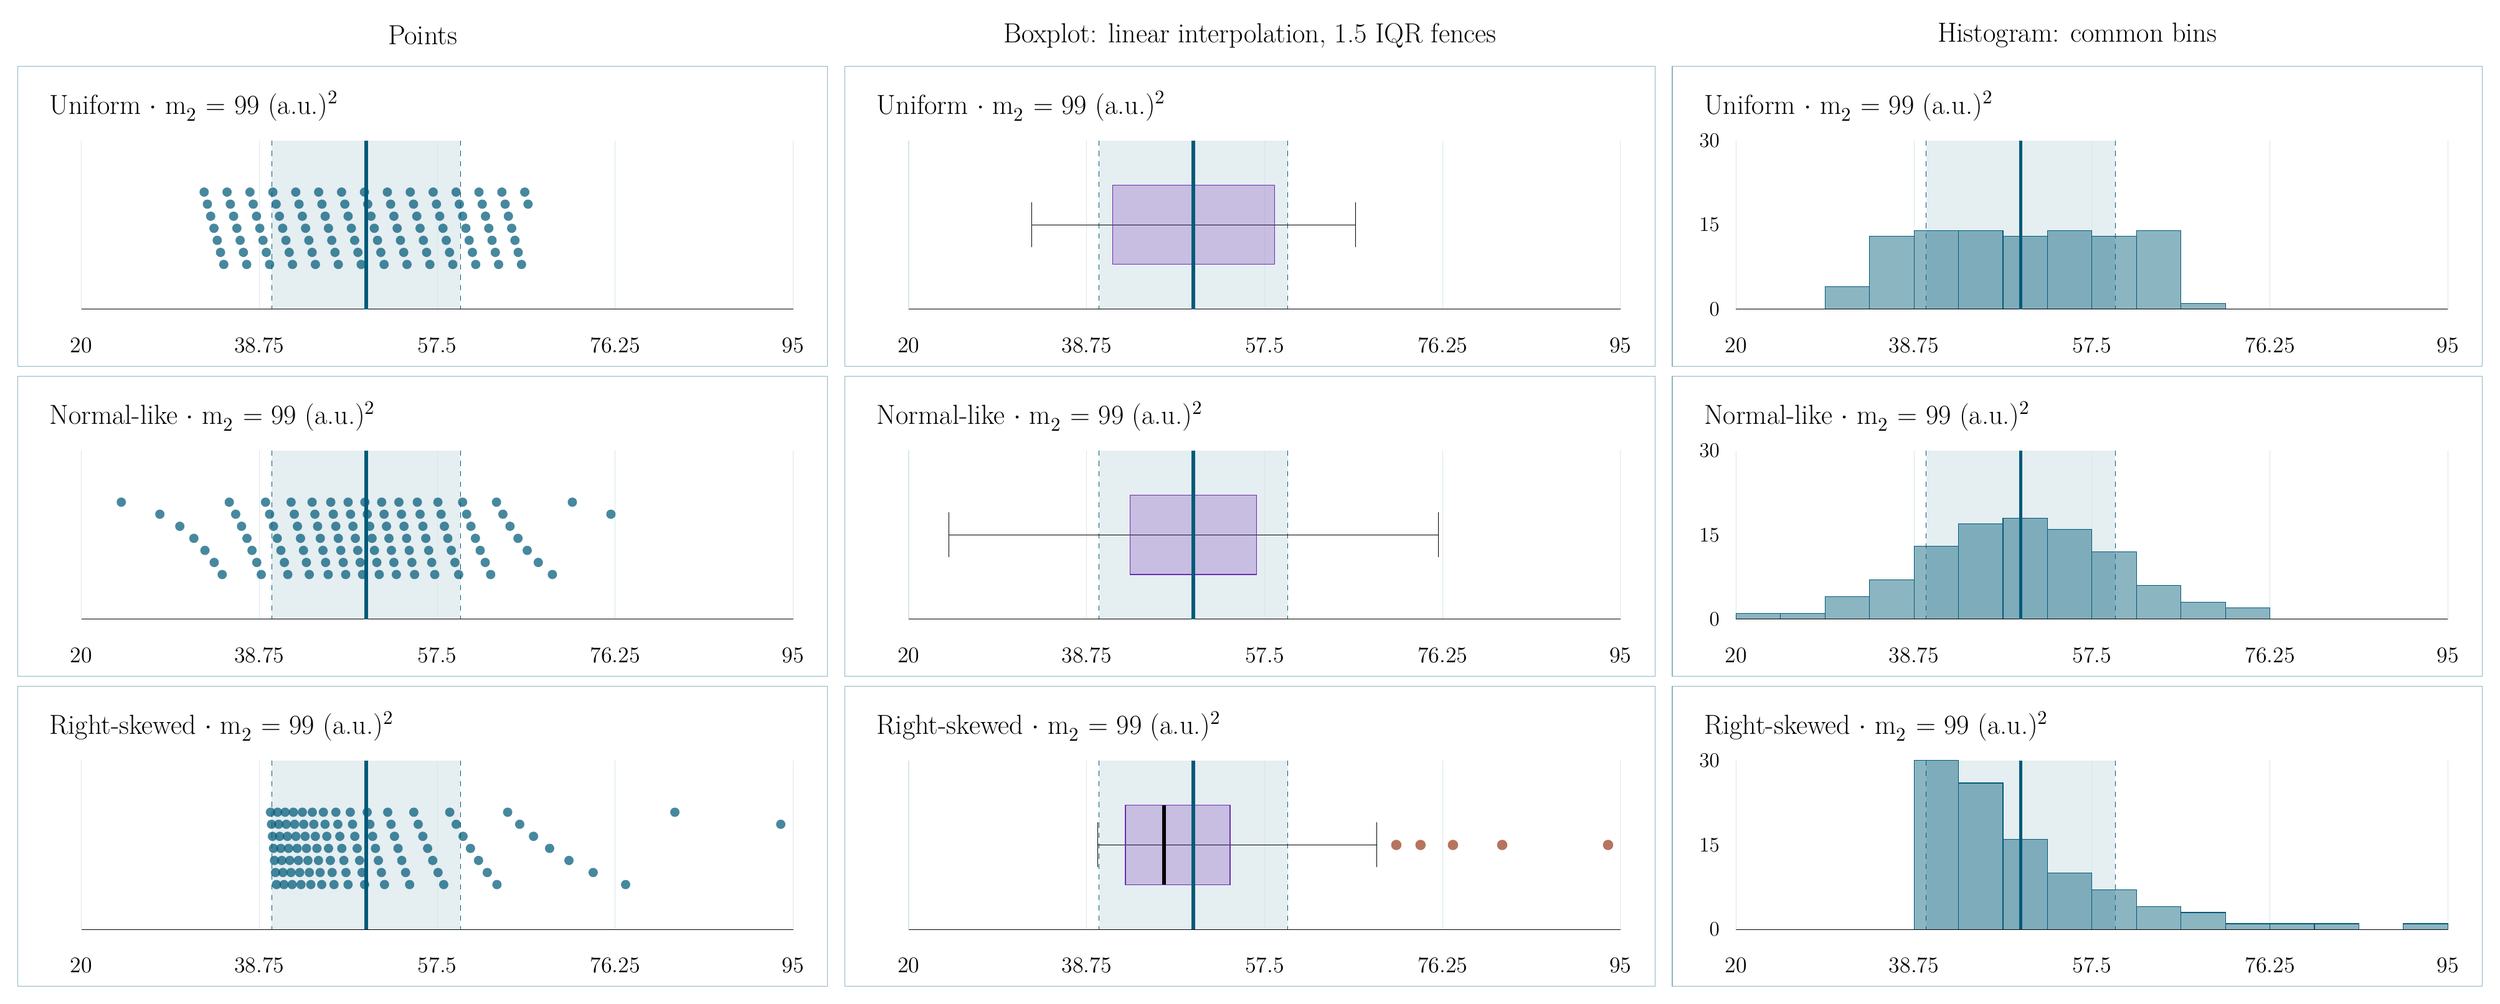
\begin{tikzpicture}[x=1pt,y=-1pt]
\node[anchor=center,font=\fontsize{16}{19}\selectfont] at (240,24) {Points};
\node[anchor=center,font=\fontsize{16}{19}\selectfont] at (720,24) {Boxplot: linear interpolation, 1.5 IQR fences};
\node[anchor=center,font=\fontsize{16}{19}\selectfont] at (1200,24) {Histogram: common bins};
\begin{scope}[shift={(0,40)}]
\path[draw=pcd1!45] (5,2) rectangle (475,176);
\node[anchor=west,font=\fontsize{16}{19}\selectfont] at (20,25) {Uniform \ensuremath{\cdot} m\ensuremath{{}_2} = 99 (a.u.)\ensuremath{{}^2}};
\path[fill=pcd1,fill opacity=.1] (152.4093584633286,45) rectangle (261.9906415366713,143);
\draw[draw=pcd1,dashed] (152.4093584633286,45) -- (152.4093584633286,143);
\draw[draw=pcd1,dashed] (261.9906415366713,45) -- (261.9906415366713,143);
\draw[draw=pcd1!15] (42,45) -- (42,143);
\node[anchor=center,font=\fontsize{13}{16}\selectfont] at (42,164) {20};
\draw[draw=pcd1!15] (145.25,45) -- (145.25,143);
\node[anchor=center,font=\fontsize{13}{16}\selectfont] at (145.25,164) {38.75};
\draw[draw=pcd1!15] (248.5,45) -- (248.5,143);
\node[anchor=center,font=\fontsize{13}{16}\selectfont] at (248.5,164) {57.5};
\draw[draw=pcd1!15] (351.75,45) -- (351.75,143);
\node[anchor=center,font=\fontsize{13}{16}\selectfont] at (351.75,164) {76.25};
\draw[draw=pcd1!15] (455,45) -- (455,143);
\node[anchor=center,font=\fontsize{13}{16}\selectfont] at (455,164) {95};
\fill[pcd1,opacity=.72] (113.24412891739694,75) circle[radius=2.7pt];
\fill[pcd1,opacity=.72] (115.14222732310145,82) circle[radius=2.7pt];
\fill[pcd1,opacity=.72] (117.04032572881144,89) circle[radius=2.7pt];
\fill[pcd1,opacity=.72] (118.93842413452143,96) circle[radius=2.7pt];
\fill[pcd1,opacity=.72] (120.83652254023141,103) circle[radius=2.7pt];
\fill[pcd1,opacity=.72] (122.7346209459414,110) circle[radius=2.7pt];
\fill[pcd1,opacity=.72] (124.63271935165137,117) circle[radius=2.7pt];
\fill[pcd1,opacity=.72] (126.53081775736136,75) circle[radius=2.7pt];
\fill[pcd1,opacity=.72] (128.42891616306582,82) circle[radius=2.7pt];
\fill[pcd1,opacity=.72] (130.32701456877584,89) circle[radius=2.7pt];
\fill[pcd1,opacity=.72] (132.2251129744858,96) circle[radius=2.7pt];
\fill[pcd1,opacity=.72] (134.1232113801958,103) circle[radius=2.7pt];
\fill[pcd1,opacity=.72] (136.02130978590577,110) circle[radius=2.7pt];
\fill[pcd1,opacity=.72] (137.9194081916158,117) circle[radius=2.7pt];
\fill[pcd1,opacity=.72] (139.81750659732575,75) circle[radius=2.7pt];
\fill[pcd1,opacity=.72] (141.71560500303025,82) circle[radius=2.7pt];
\fill[pcd1,opacity=.72] (143.61370340874024,89) circle[radius=2.7pt];
\fill[pcd1,opacity=.72] (145.51180181445022,96) circle[radius=2.7pt];
\fill[pcd1,opacity=.72] (147.4099002201602,103) circle[radius=2.7pt];
\fill[pcd1,opacity=.72] (149.3079986258702,110) circle[radius=2.7pt];
\fill[pcd1,opacity=.72] (151.20609703158019,117) circle[radius=2.7pt];
\fill[pcd1,opacity=.72] (153.10419543729017,75) circle[radius=2.7pt];
\fill[pcd1,opacity=.72] (155.00229384299465,82) circle[radius=2.7pt];
\fill[pcd1,opacity=.72] (156.90039224870463,89) circle[radius=2.7pt];
\fill[pcd1,opacity=.72] (158.79849065441462,96) circle[radius=2.7pt];
\fill[pcd1,opacity=.72] (160.6965890601246,103) circle[radius=2.7pt];
\fill[pcd1,opacity=.72] (162.59468746583457,110) circle[radius=2.7pt];
\fill[pcd1,opacity=.72] (164.49278587154458,117) circle[radius=2.7pt];
\fill[pcd1,opacity=.72] (166.39088427725454,75) circle[radius=2.7pt];
\fill[pcd1,opacity=.72] (168.28898268295902,82) circle[radius=2.7pt];
\fill[pcd1,opacity=.72] (170.18708108866903,89) circle[radius=2.7pt];
\fill[pcd1,opacity=.72] (172.085179494379,96) circle[radius=2.7pt];
\fill[pcd1,opacity=.72] (173.98327790008898,103) circle[radius=2.7pt];
\fill[pcd1,opacity=.72] (175.88137630579897,110) circle[radius=2.7pt];
\fill[pcd1,opacity=.72] (177.77947471150895,117) circle[radius=2.7pt];
\fill[pcd1,opacity=.72] (179.67757311721897,75) circle[radius=2.7pt];
\fill[pcd1,opacity=.72] (181.57567152292344,82) circle[radius=2.7pt];
\fill[pcd1,opacity=.72] (183.47376992863343,89) circle[radius=2.7pt];
\fill[pcd1,opacity=.72] (185.37186833434342,96) circle[radius=2.7pt];
\fill[pcd1,opacity=.72] (187.2699667400534,103) circle[radius=2.7pt];
\fill[pcd1,opacity=.72] (189.1680651457634,110) circle[radius=2.7pt];
\fill[pcd1,opacity=.72] (191.06616355147338,117) circle[radius=2.7pt];
\fill[pcd1,opacity=.72] (192.96426195718337,75) circle[radius=2.7pt];
\fill[pcd1,opacity=.72] (194.8623603628878,82) circle[radius=2.7pt];
\fill[pcd1,opacity=.72] (196.76045876859783,89) circle[radius=2.7pt];
\fill[pcd1,opacity=.72] (198.65855717430782,96) circle[radius=2.7pt];
\fill[pcd1,opacity=.72] (200.55665558001778,103) circle[radius=2.7pt];
\fill[pcd1,opacity=.72] (202.4547539857278,110) circle[radius=2.7pt];
\fill[pcd1,opacity=.72] (204.35285239143775,117) circle[radius=2.7pt];
\fill[pcd1,opacity=.72] (206.25095079714774,75) circle[radius=2.7pt];
\fill[pcd1,opacity=.72] (208.14904920285224,82) circle[radius=2.7pt];
\fill[pcd1,opacity=.72] (210.04714760856223,89) circle[radius=2.7pt];
\fill[pcd1,opacity=.72] (211.94524601427224,96) circle[radius=2.7pt];
\fill[pcd1,opacity=.72] (213.8433444199822,103) circle[radius=2.7pt];
\fill[pcd1,opacity=.72] (215.74144282569222,110) circle[radius=2.7pt];
\fill[pcd1,opacity=.72] (217.63954123140218,117) circle[radius=2.7pt];
\fill[pcd1,opacity=.72] (219.53763963711216,75) circle[radius=2.7pt];
\fill[pcd1,opacity=.72] (221.43573804281664,82) circle[radius=2.7pt];
\fill[pcd1,opacity=.72] (223.33383644852663,89) circle[radius=2.7pt];
\fill[pcd1,opacity=.72] (225.2319348542366,96) circle[radius=2.7pt];
\fill[pcd1,opacity=.72] (227.13003325994657,103) circle[radius=2.7pt];
\fill[pcd1,opacity=.72] (229.0281316656566,110) circle[radius=2.7pt];
\fill[pcd1,opacity=.72] (230.92623007136655,117) circle[radius=2.7pt];
\fill[pcd1,opacity=.72] (232.82432847707656,75) circle[radius=2.7pt];
\fill[pcd1,opacity=.72] (234.722426882781,82) circle[radius=2.7pt];
\fill[pcd1,opacity=.72] (236.62052528849105,89) circle[radius=2.7pt];
\fill[pcd1,opacity=.72] (238.51862369420104,96) circle[radius=2.7pt];
\fill[pcd1,opacity=.72] (240.416722099911,103) circle[radius=2.7pt];
\fill[pcd1,opacity=.72] (242.31482050562101,110) circle[radius=2.7pt];
\fill[pcd1,opacity=.72] (244.21291891133097,117) circle[radius=2.7pt];
\fill[pcd1,opacity=.72] (246.11101731704096,75) circle[radius=2.7pt];
\fill[pcd1,opacity=.72] (248.00911572274543,82) circle[radius=2.7pt];
\fill[pcd1,opacity=.72] (249.90721412845545,89) circle[radius=2.7pt];
\fill[pcd1,opacity=.72] (251.8053125341654,96) circle[radius=2.7pt];
\fill[pcd1,opacity=.72] (253.7034109398754,103) circle[radius=2.7pt];
\fill[pcd1,opacity=.72] (255.6015093455854,110) circle[radius=2.7pt];
\fill[pcd1,opacity=.72] (257.49960775129534,117) circle[radius=2.7pt];
\fill[pcd1,opacity=.72] (259.39770615700536,75) circle[radius=2.7pt];
\fill[pcd1,opacity=.72] (261.2958045627098,82) circle[radius=2.7pt];
\fill[pcd1,opacity=.72] (263.1939029684198,89) circle[radius=2.7pt];
\fill[pcd1,opacity=.72] (265.09200137412984,96) circle[radius=2.7pt];
\fill[pcd1,opacity=.72] (266.9900997798398,103) circle[radius=2.7pt];
\fill[pcd1,opacity=.72] (268.88819818554975,110) circle[radius=2.7pt];
\fill[pcd1,opacity=.72] (270.78629659125977,117) circle[radius=2.7pt];
\fill[pcd1,opacity=.72] (272.6843949969698,75) circle[radius=2.7pt];
\fill[pcd1,opacity=.72] (274.58249340267423,82) circle[radius=2.7pt];
\fill[pcd1,opacity=.72] (276.48059180838425,89) circle[radius=2.7pt];
\fill[pcd1,opacity=.72] (278.3786902140942,96) circle[radius=2.7pt];
\fill[pcd1,opacity=.72] (280.27678861980417,103) circle[radius=2.7pt];
\fill[pcd1,opacity=.72] (282.1748870255142,110) circle[radius=2.7pt];
\fill[pcd1,opacity=.72] (284.0729854312242,117) circle[radius=2.7pt];
\fill[pcd1,opacity=.72] (285.97108383693416,75) circle[radius=2.7pt];
\fill[pcd1,opacity=.72] (287.86918224263866,82) circle[radius=2.7pt];
\fill[pcd1,opacity=.72] (289.7672806483487,89) circle[radius=2.7pt];
\fill[pcd1,opacity=.72] (291.6653790540587,96) circle[radius=2.7pt];
\fill[pcd1,opacity=.72] (293.5634774597686,103) circle[radius=2.7pt];
\fill[pcd1,opacity=.72] (295.4615758654786,110) circle[radius=2.7pt];
\fill[pcd1,opacity=.72] (297.3596742711886,117) circle[radius=2.7pt];
\fill[pcd1,opacity=.72] (299.25777267689307,75) circle[radius=2.7pt];
\fill[pcd1,opacity=.72] (301.155871082603,82) circle[radius=2.7pt];
\draw[draw=black] (42,143) -- (455,143);
\draw[draw=pcd1,line width=2pt] (207.19999999999996,45) -- (207.19999999999996,143);
\end{scope}
\begin{scope}[shift={(480,40)}]
\path[draw=pcd1!45] (5,2) rectangle (475,176);
\node[anchor=west,font=\fontsize{16}{19}\selectfont] at (20,25) {Uniform \ensuremath{\cdot} m\ensuremath{{}_2} = 99 (a.u.)\ensuremath{{}^2}};
\path[fill=pcd1,fill opacity=.1] (152.4093584633286,45) rectangle (261.9906415366713,143);
\draw[draw=pcd1,dashed] (152.4093584633286,45) -- (152.4093584633286,143);
\draw[draw=pcd1,dashed] (261.9906415366713,45) -- (261.9906415366713,143);
\draw[draw=pcd1!15] (42,45) -- (42,143);
\node[anchor=center,font=\fontsize{13}{16}\selectfont] at (42,164) {20};
\draw[draw=pcd1!15] (145.25,45) -- (145.25,143);
\node[anchor=center,font=\fontsize{13}{16}\selectfont] at (145.25,164) {38.75};
\draw[draw=pcd1!15] (248.5,45) -- (248.5,143);
\node[anchor=center,font=\fontsize{13}{16}\selectfont] at (248.5,164) {57.5};
\draw[draw=pcd1!15] (351.75,45) -- (351.75,143);
\node[anchor=center,font=\fontsize{13}{16}\selectfont] at (351.75,164) {76.25};
\draw[draw=pcd1!15] (455,45) -- (455,143);
\node[anchor=center,font=\fontsize{13}{16}\selectfont] at (455,164) {95};
\draw[draw=black] (113.24412891739694,94) -- (301.155871082603,94);
\path[fill=pcd2,fill opacity=.25,draw=pcd2] (160.22206445869708,71) rectangle (254.1779355413029,117);
\draw[draw=black,line width=2pt] (207.20000000000002,71) -- (207.20000000000002,117);
\draw[draw=black] (113.24412891739694,81) -- (113.24412891739694,107);
\draw[draw=black] (301.155871082603,81) -- (301.155871082603,107);
\draw[draw=black] (42,143) -- (455,143);
\draw[draw=pcd1,line width=2pt] (207.19999999999996,45) -- (207.19999999999996,143);
\end{scope}
\begin{scope}[shift={(960,40)}]
\path[draw=pcd1!45] (5,2) rectangle (475,176);
\node[anchor=west,font=\fontsize{16}{19}\selectfont] at (20,25) {Uniform \ensuremath{\cdot} m\ensuremath{{}_2} = 99 (a.u.)\ensuremath{{}^2}};
\path[fill=pcd1,fill opacity=.1] (152.4093584633286,45) rectangle (261.9906415366713,143);
\draw[draw=pcd1,dashed] (152.4093584633286,45) -- (152.4093584633286,143);
\draw[draw=pcd1,dashed] (261.9906415366713,45) -- (261.9906415366713,143);
\draw[draw=pcd1!15] (42,45) -- (42,143);
\node[anchor=center,font=\fontsize{13}{16}\selectfont] at (42,164) {20};
\draw[draw=pcd1!15] (145.25,45) -- (145.25,143);
\node[anchor=center,font=\fontsize{13}{16}\selectfont] at (145.25,164) {38.75};
\draw[draw=pcd1!15] (248.5,45) -- (248.5,143);
\node[anchor=center,font=\fontsize{13}{16}\selectfont] at (248.5,164) {57.5};
\draw[draw=pcd1!15] (351.75,45) -- (351.75,143);
\node[anchor=center,font=\fontsize{13}{16}\selectfont] at (351.75,164) {76.25};
\draw[draw=pcd1!15] (455,45) -- (455,143);
\node[anchor=center,font=\fontsize{13}{16}\selectfont] at (455,164) {95};
\path[fill=pcd1,fill opacity=.45,draw=pcd1] (42,143) rectangle (67.8125,143);
\path[fill=pcd1,fill opacity=.45,draw=pcd1] (67.8125,143) rectangle (93.625,143);
\path[fill=pcd1,fill opacity=.45,draw=pcd1] (93.625,129.93333333333334) rectangle (119.4375,143);
\path[fill=pcd1,fill opacity=.45,draw=pcd1] (119.4375,100.53333333333333) rectangle (145.25,143);
\path[fill=pcd1,fill opacity=.45,draw=pcd1] (145.25,97.26666666666667) rectangle (171.0625,143);
\path[fill=pcd1,fill opacity=.45,draw=pcd1] (171.0625,97.26666666666667) rectangle (196.875,143);
\path[fill=pcd1,fill opacity=.45,draw=pcd1] (196.875,100.53333333333333) rectangle (222.6875,143);
\path[fill=pcd1,fill opacity=.45,draw=pcd1] (222.6875,97.26666666666667) rectangle (248.5,143);
\path[fill=pcd1,fill opacity=.45,draw=pcd1] (248.5,100.53333333333333) rectangle (274.3125,143);
\path[fill=pcd1,fill opacity=.45,draw=pcd1] (274.3125,97.26666666666667) rectangle (300.125,143);
\path[fill=pcd1,fill opacity=.45,draw=pcd1] (300.125,139.73333333333332) rectangle (325.9375,143);
\path[fill=pcd1,fill opacity=.45,draw=pcd1] (325.9375,143) rectangle (351.75,143);
\path[fill=pcd1,fill opacity=.45,draw=pcd1] (351.75,143) rectangle (377.5625,143);
\path[fill=pcd1,fill opacity=.45,draw=pcd1] (377.5625,143) rectangle (403.375,143);
\path[fill=pcd1,fill opacity=.45,draw=pcd1] (403.375,143) rectangle (429.1875,143);
\path[fill=pcd1,fill opacity=.45,draw=pcd1] (429.1875,143) rectangle (455,143);
\node[anchor=east,font=\fontsize{12}{15}\selectfont] at (36,143) {0};
\node[anchor=east,font=\fontsize{12}{15}\selectfont] at (36,94) {15};
\node[anchor=east,font=\fontsize{12}{15}\selectfont] at (36,45) {30};
\draw[draw=black] (42,143) -- (455,143);
\draw[draw=pcd1,line width=2pt] (207.19999999999996,45) -- (207.19999999999996,143);
\end{scope}
\begin{scope}[shift={(0,220)}]
\path[draw=pcd1!45] (5,2) rectangle (475,176);
\node[anchor=west,font=\fontsize{16}{19}\selectfont] at (20,25) {Normal-like \ensuremath{\cdot} m\ensuremath{{}_2} = 99 (a.u.)\ensuremath{{}^2}};
\path[fill=pcd1,fill opacity=.1] (152.40935846332863,45) rectangle (261.9906415366714,143);
\draw[draw=pcd1,dashed] (152.40935846332863,45) -- (152.40935846332863,143);
\draw[draw=pcd1,dashed] (261.9906415366714,45) -- (261.9906415366714,143);
\draw[draw=pcd1!15] (42,45) -- (42,143);
\node[anchor=center,font=\fontsize{13}{16}\selectfont] at (42,164) {20};
\draw[draw=pcd1!15] (145.25,45) -- (145.25,143);
\node[anchor=center,font=\fontsize{13}{16}\selectfont] at (145.25,164) {38.75};
\draw[draw=pcd1!15] (248.5,45) -- (248.5,143);
\node[anchor=center,font=\fontsize{13}{16}\selectfont] at (248.5,164) {57.5};
\draw[draw=pcd1!15] (351.75,45) -- (351.75,143);
\node[anchor=center,font=\fontsize{13}{16}\selectfont] at (351.75,164) {76.25};
\draw[draw=pcd1!15] (455,45) -- (455,143);
\node[anchor=center,font=\fontsize{13}{16}\selectfont] at (455,164) {95};
\fill[pcd1,opacity=.72] (65.16454133626237,75) circle[radius=2.7pt];
\fill[pcd1,opacity=.72] (87.53765215058463,82) circle[radius=2.7pt];
\fill[pcd1,opacity=.72] (99.12436660107437,89) circle[radius=2.7pt];
\fill[pcd1,opacity=.72] (107.28826938338861,96) circle[radius=2.7pt];
\fill[pcd1,opacity=.72] (113.7129855211349,103) circle[radius=2.7pt];
\fill[pcd1,opacity=.72] (119.0730051912103,110) circle[radius=2.7pt];
\fill[pcd1,opacity=.72] (123.70993496528129,117) circle[radius=2.7pt];
\fill[pcd1,opacity=.72] (127.82187022489454,75) circle[radius=2.7pt];
\fill[pcd1,opacity=.72] (131.53442809166978,82) circle[radius=2.7pt];
\fill[pcd1,opacity=.72] (134.93251509506104,89) circle[radius=2.7pt];
\fill[pcd1,opacity=.72] (138.07634270918393,96) circle[radius=2.7pt];
\fill[pcd1,opacity=.72] (141.01024094780104,103) circle[radius=2.7pt];
\fill[pcd1,opacity=.72] (143.76784568754908,110) circle[radius=2.7pt];
\fill[pcd1,opacity=.72] (146.37531884246346,117) circle[radius=2.7pt];
\fill[pcd1,opacity=.72] (148.85343600881788,75) circle[radius=2.7pt];
\fill[pcd1,opacity=.72] (151.21898956004614,82) circle[radius=2.7pt];
\fill[pcd1,opacity=.72] (153.48576081178732,89) circle[radius=2.7pt];
\fill[pcd1,opacity=.72] (155.66521140319736,96) circle[radius=2.7pt];
\fill[pcd1,opacity=.72] (157.7669862283159,103) circle[radius=2.7pt];
\fill[pcd1,opacity=.72] (159.7992865920125,110) circle[radius=2.7pt];
\fill[pcd1,opacity=.72] (161.76915195659856,117) circle[radius=2.7pt];
\fill[pcd1,opacity=.72] (163.68267600478754,75) circle[radius=2.7pt];
\fill[pcd1,opacity=.72] (165.54517465782482,82) circle[radius=2.7pt];
\fill[pcd1,opacity=.72] (167.36131838621117,89) circle[radius=2.7pt];
\fill[pcd1,opacity=.72] (169.1352375982878,96) circle[radius=2.7pt];
\fill[pcd1,opacity=.72] (170.87060746462737,103) circle[radius=2.7pt];
\fill[pcd1,opacity=.72] (172.5707168478382,110) circle[radius=2.7pt];
\fill[pcd1,opacity=.72] (174.2385248135968,117) circle[radius=2.7pt];
\fill[pcd1,opacity=.72] (175.87670734235186,75) circle[radius=2.7pt];
\fill[pcd1,opacity=.72] (177.4876962383739,82) circle[radius=2.7pt];
\fill[pcd1,opacity=.72] (179.07371177394688,89) circle[radius=2.7pt];
\fill[pcd1,opacity=.72] (180.63679026512506,96) circle[radius=2.7pt];
\fill[pcd1,opacity=.72] (182.17880751793538,103) circle[radius=2.7pt];
\fill[pcd1,opacity=.72] (183.7014988885424,110) circle[radius=2.7pt];
\fill[pcd1,opacity=.72] (185.20647655075038,117) circle[radius=2.7pt];
\fill[pcd1,opacity=.72] (186.69524444809016,75) circle[radius=2.7pt];
\fill[pcd1,opacity=.72] (188.16921131713553,82) circle[radius=2.7pt];
\fill[pcd1,opacity=.72] (189.62970209763023,89) circle[radius=2.7pt];
\fill[pcd1,opacity=.72] (191.07796798874614,96) circle[radius=2.7pt];
\fill[pcd1,opacity=.72] (192.51519536587472,103) circle[radius=2.7pt];
\fill[pcd1,opacity=.72] (193.94251373685682,110) circle[radius=2.7pt];
\fill[pcd1,opacity=.72] (195.36100288752172,117) circle[radius=2.7pt];
\fill[pcd1,opacity=.72] (196.77169934342442,75) circle[radius=2.7pt];
\fill[pcd1,opacity=.72] (198.17560225582272,82) circle[radius=2.7pt];
\fill[pcd1,opacity=.72] (199.57367880477972,89) circle[radius=2.7pt];
\fill[pcd1,opacity=.72] (200.96686920014255,96) circle[radius=2.7pt];
\fill[pcd1,opacity=.72] (202.3560913510083,103) circle[radius=2.7pt];
\fill[pcd1,opacity=.72] (203.74224526671262,110) circle[radius=2.7pt];
\fill[pcd1,opacity=.72] (205.1262172457786,117) circle[radius=2.7pt];
\fill[pcd1,opacity=.72] (206.50888390477604,75) circle[radius=2.7pt];
\fill[pcd1,opacity=.72] (207.89111609522396,82) circle[radius=2.7pt];
\fill[pcd1,opacity=.72] (209.27378275422137,89) circle[radius=2.7pt];
\fill[pcd1,opacity=.72] (210.6577547332874,96) circle[radius=2.7pt];
\fill[pcd1,opacity=.72] (212.0439086489917,103) circle[radius=2.7pt];
\fill[pcd1,opacity=.72] (213.43313079985745,110) circle[radius=2.7pt];
\fill[pcd1,opacity=.72] (214.8263211952203,117) circle[radius=2.7pt];
\fill[pcd1,opacity=.72] (216.22439774417728,75) circle[radius=2.7pt];
\fill[pcd1,opacity=.72] (217.62830065657556,82) circle[radius=2.7pt];
\fill[pcd1,opacity=.72] (219.03899711247826,89) circle[radius=2.7pt];
\fill[pcd1,opacity=.72] (220.45748626314318,96) circle[radius=2.7pt];
\fill[pcd1,opacity=.72] (221.8848046341253,103) circle[radius=2.7pt];
\fill[pcd1,opacity=.72] (223.32203201125384,110) circle[radius=2.7pt];
\fill[pcd1,opacity=.72] (224.77029790236978,117) circle[radius=2.7pt];
\fill[pcd1,opacity=.72] (226.23078868286447,75) circle[radius=2.7pt];
\fill[pcd1,opacity=.72] (227.70475555190984,82) circle[radius=2.7pt];
\fill[pcd1,opacity=.72] (229.1935234492496,89) circle[radius=2.7pt];
\fill[pcd1,opacity=.72] (230.6985011114576,96) circle[radius=2.7pt];
\fill[pcd1,opacity=.72] (232.22119248206462,103) circle[radius=2.7pt];
\fill[pcd1,opacity=.72] (233.76320973487495,110) circle[radius=2.7pt];
\fill[pcd1,opacity=.72] (235.3262882260531,117) circle[radius=2.7pt];
\fill[pcd1,opacity=.72] (236.91230376162608,75) circle[radius=2.7pt];
\fill[pcd1,opacity=.72] (238.52329265764814,82) circle[radius=2.7pt];
\fill[pcd1,opacity=.72] (240.16147518640324,89) circle[radius=2.7pt];
\fill[pcd1,opacity=.72] (241.8292831521618,96) circle[radius=2.7pt];
\fill[pcd1,opacity=.72] (243.52939253537264,103) circle[radius=2.7pt];
\fill[pcd1,opacity=.72] (245.2647624017122,110) circle[radius=2.7pt];
\fill[pcd1,opacity=.72] (247.03868161378887,117) circle[radius=2.7pt];
\fill[pcd1,opacity=.72] (248.8548253421752,75) circle[radius=2.7pt];
\fill[pcd1,opacity=.72] (250.71732399521247,82) circle[radius=2.7pt];
\fill[pcd1,opacity=.72] (252.63084804340141,89) circle[radius=2.7pt];
\fill[pcd1,opacity=.72] (254.60071340798754,96) circle[radius=2.7pt];
\fill[pcd1,opacity=.72] (256.6330137716841,103) circle[radius=2.7pt];
\fill[pcd1,opacity=.72] (258.7347885968027,110) circle[radius=2.7pt];
\fill[pcd1,opacity=.72] (260.9142391882127,117) circle[radius=2.7pt];
\fill[pcd1,opacity=.72] (263.18101043995387,75) circle[radius=2.7pt];
\fill[pcd1,opacity=.72] (265.5465639911821,82) circle[radius=2.7pt];
\fill[pcd1,opacity=.72] (268.0246811575365,89) circle[radius=2.7pt];
\fill[pcd1,opacity=.72] (270.63215431245095,96) circle[radius=2.7pt];
\fill[pcd1,opacity=.72] (273.389759052199,103) circle[radius=2.7pt];
\fill[pcd1,opacity=.72] (276.3236572908161,110) circle[radius=2.7pt];
\fill[pcd1,opacity=.72] (279.46748490493894,117) circle[radius=2.7pt];
\fill[pcd1,opacity=.72] (282.86557190833025,75) circle[radius=2.7pt];
\fill[pcd1,opacity=.72] (286.5781297751055,82) circle[radius=2.7pt];
\fill[pcd1,opacity=.72] (290.6900650347187,89) circle[radius=2.7pt];
\fill[pcd1,opacity=.72] (295.3269948087898,96) circle[radius=2.7pt];
\fill[pcd1,opacity=.72] (300.6870144788651,103) circle[radius=2.7pt];
\fill[pcd1,opacity=.72] (307.1117306166114,110) circle[radius=2.7pt];
\fill[pcd1,opacity=.72] (315.27563339892566,117) circle[radius=2.7pt];
\fill[pcd1,opacity=.72] (326.86234784941536,75) circle[radius=2.7pt];
\fill[pcd1,opacity=.72] (349.2354586637376,82) circle[radius=2.7pt];
\draw[draw=black] (42,143) -- (455,143);
\draw[draw=pcd1,line width=2pt] (207.20000000000002,45) -- (207.20000000000002,143);
\end{scope}
\begin{scope}[shift={(480,220)}]
\path[draw=pcd1!45] (5,2) rectangle (475,176);
\node[anchor=west,font=\fontsize{16}{19}\selectfont] at (20,25) {Normal-like \ensuremath{\cdot} m\ensuremath{{}_2} = 99 (a.u.)\ensuremath{{}^2}};
\path[fill=pcd1,fill opacity=.1] (152.40935846332863,45) rectangle (261.9906415366714,143);
\draw[draw=pcd1,dashed] (152.40935846332863,45) -- (152.40935846332863,143);
\draw[draw=pcd1,dashed] (261.9906415366714,45) -- (261.9906415366714,143);
\draw[draw=pcd1!15] (42,45) -- (42,143);
\node[anchor=center,font=\fontsize{13}{16}\selectfont] at (42,164) {20};
\draw[draw=pcd1!15] (145.25,45) -- (145.25,143);
\node[anchor=center,font=\fontsize{13}{16}\selectfont] at (145.25,164) {38.75};
\draw[draw=pcd1!15] (248.5,45) -- (248.5,143);
\node[anchor=center,font=\fontsize{13}{16}\selectfont] at (248.5,164) {57.5};
\draw[draw=pcd1!15] (351.75,45) -- (351.75,143);
\node[anchor=center,font=\fontsize{13}{16}\selectfont] at (351.75,164) {76.25};
\draw[draw=pcd1!15] (455,45) -- (455,143);
\node[anchor=center,font=\fontsize{13}{16}\selectfont] at (455,164) {95};
\draw[draw=black] (65.16454133626237,94) -- (349.2354586637376,94);
\path[fill=pcd2,fill opacity=.25,draw=pcd2] (170.43676499804246,71) rectangle (243.96323500195754,117);
\draw[draw=black,line width=2pt] (207.20000000000002,71) -- (207.20000000000002,117);
\draw[draw=black] (65.16454133626237,81) -- (65.16454133626237,107);
\draw[draw=black] (349.2354586637376,81) -- (349.2354586637376,107);
\draw[draw=black] (42,143) -- (455,143);
\draw[draw=pcd1,line width=2pt] (207.20000000000002,45) -- (207.20000000000002,143);
\end{scope}
\begin{scope}[shift={(960,220)}]
\path[draw=pcd1!45] (5,2) rectangle (475,176);
\node[anchor=west,font=\fontsize{16}{19}\selectfont] at (20,25) {Normal-like \ensuremath{\cdot} m\ensuremath{{}_2} = 99 (a.u.)\ensuremath{{}^2}};
\path[fill=pcd1,fill opacity=.1] (152.40935846332863,45) rectangle (261.9906415366714,143);
\draw[draw=pcd1,dashed] (152.40935846332863,45) -- (152.40935846332863,143);
\draw[draw=pcd1,dashed] (261.9906415366714,45) -- (261.9906415366714,143);
\draw[draw=pcd1!15] (42,45) -- (42,143);
\node[anchor=center,font=\fontsize{13}{16}\selectfont] at (42,164) {20};
\draw[draw=pcd1!15] (145.25,45) -- (145.25,143);
\node[anchor=center,font=\fontsize{13}{16}\selectfont] at (145.25,164) {38.75};
\draw[draw=pcd1!15] (248.5,45) -- (248.5,143);
\node[anchor=center,font=\fontsize{13}{16}\selectfont] at (248.5,164) {57.5};
\draw[draw=pcd1!15] (351.75,45) -- (351.75,143);
\node[anchor=center,font=\fontsize{13}{16}\selectfont] at (351.75,164) {76.25};
\draw[draw=pcd1!15] (455,45) -- (455,143);
\node[anchor=center,font=\fontsize{13}{16}\selectfont] at (455,164) {95};
\path[fill=pcd1,fill opacity=.45,draw=pcd1] (42,139.73333333333332) rectangle (67.8125,143);
\path[fill=pcd1,fill opacity=.45,draw=pcd1] (67.8125,139.73333333333332) rectangle (93.625,143);
\path[fill=pcd1,fill opacity=.45,draw=pcd1] (93.625,129.93333333333334) rectangle (119.4375,143);
\path[fill=pcd1,fill opacity=.45,draw=pcd1] (119.4375,120.13333333333333) rectangle (145.25,143);
\path[fill=pcd1,fill opacity=.45,draw=pcd1] (145.25,100.53333333333333) rectangle (171.0625,143);
\path[fill=pcd1,fill opacity=.45,draw=pcd1] (171.0625,87.46666666666667) rectangle (196.875,143);
\path[fill=pcd1,fill opacity=.45,draw=pcd1] (196.875,84.2) rectangle (222.6875,143);
\path[fill=pcd1,fill opacity=.45,draw=pcd1] (222.6875,90.73333333333333) rectangle (248.5,143);
\path[fill=pcd1,fill opacity=.45,draw=pcd1] (248.5,103.8) rectangle (274.3125,143);
\path[fill=pcd1,fill opacity=.45,draw=pcd1] (274.3125,123.4) rectangle (300.125,143);
\path[fill=pcd1,fill opacity=.45,draw=pcd1] (300.125,133.2) rectangle (325.9375,143);
\path[fill=pcd1,fill opacity=.45,draw=pcd1] (325.9375,136.46666666666667) rectangle (351.75,143);
\path[fill=pcd1,fill opacity=.45,draw=pcd1] (351.75,143) rectangle (377.5625,143);
\path[fill=pcd1,fill opacity=.45,draw=pcd1] (377.5625,143) rectangle (403.375,143);
\path[fill=pcd1,fill opacity=.45,draw=pcd1] (403.375,143) rectangle (429.1875,143);
\path[fill=pcd1,fill opacity=.45,draw=pcd1] (429.1875,143) rectangle (455,143);
\node[anchor=east,font=\fontsize{12}{15}\selectfont] at (36,143) {0};
\node[anchor=east,font=\fontsize{12}{15}\selectfont] at (36,94) {15};
\node[anchor=east,font=\fontsize{12}{15}\selectfont] at (36,45) {30};
\draw[draw=black] (42,143) -- (455,143);
\draw[draw=pcd1,line width=2pt] (207.20000000000002,45) -- (207.20000000000002,143);
\end{scope}
\begin{scope}[shift={(0,400)}]
\path[draw=pcd1!45] (5,2) rectangle (475,176);
\node[anchor=west,font=\fontsize{16}{19}\selectfont] at (20,25) {Right-skewed \ensuremath{\cdot} m\ensuremath{{}_2} = 99 (a.u.)\ensuremath{{}^2}};
\path[fill=pcd1,fill opacity=.1] (152.40935846332886,45) rectangle (261.9906415366711,143);
\draw[draw=pcd1,dashed] (152.40935846332886,45) -- (152.40935846332886,143);
\draw[draw=pcd1,dashed] (261.9906415366711,45) -- (261.9906415366711,143);
\draw[draw=pcd1!15] (42,45) -- (42,143);
\node[anchor=center,font=\fontsize{13}{16}\selectfont] at (42,164) {20};
\draw[draw=pcd1!15] (145.25,45) -- (145.25,143);
\node[anchor=center,font=\fontsize{13}{16}\selectfont] at (145.25,164) {38.75};
\draw[draw=pcd1!15] (248.5,45) -- (248.5,143);
\node[anchor=center,font=\fontsize{13}{16}\selectfont] at (248.5,164) {57.5};
\draw[draw=pcd1!15] (351.75,45) -- (351.75,143);
\node[anchor=center,font=\fontsize{13}{16}\selectfont] at (351.75,164) {76.25};
\draw[draw=pcd1!15] (455,45) -- (455,143);
\node[anchor=center,font=\fontsize{13}{16}\selectfont] at (455,164) {95};
\fill[pcd1,opacity=.72] (151.74905333266133,75) circle[radius=2.7pt];
\fill[pcd1,opacity=.72] (152.31395571301317,82) circle[radius=2.7pt];
\fill[pcd1,opacity=.72] (152.8846225028966,89) circle[radius=2.7pt];
\fill[pcd1,opacity=.72] (153.4611725592456,96) circle[radius=2.7pt];
\fill[pcd1,opacity=.72] (154.04372845340623,103) circle[radius=2.7pt];
\fill[pcd1,opacity=.72] (154.63241662752557,110) circle[radius=2.7pt];
\fill[pcd1,opacity=.72] (155.22736755930603,117) circle[radius=2.7pt];
\fill[pcd1,opacity=.72] (155.8287159355586,75) circle[radius=2.7pt];
\fill[pcd1,opacity=.72] (156.4366008352228,82) circle[radius=2.7pt];
\fill[pcd1,opacity=.72] (157.0511659224521,89) circle[radius=2.7pt];
\fill[pcd1,opacity=.72] (157.67255965038294,96) circle[radius=2.7pt];
\fill[pcd1,opacity=.72] (158.3009354764065,103) circle[radius=2.7pt];
\fill[pcd1,opacity=.72] (158.93645208964392,110) circle[radius=2.7pt];
\fill[pcd1,opacity=.72] (159.5792736514773,117) circle[radius=2.7pt];
\fill[pcd1,opacity=.72] (160.22957005010642,75) circle[radius=2.7pt];
\fill[pcd1,opacity=.72] (160.88751717007247,82) circle[radius=2.7pt];
\fill[pcd1,opacity=.72] (161.55329717777346,89) circle[radius=2.7pt];
\fill[pcd1,opacity=.72] (162.22709882426457,96) circle[radius=2.7pt];
\fill[pcd1,opacity=.72] (162.90911776645657,103) circle[radius=2.7pt];
\fill[pcd1,opacity=.72] (163.59955690818776,110) circle[radius=2.7pt];
\fill[pcd1,opacity=.72] (164.2986267625626,117) circle[radius=2.7pt];
\fill[pcd1,opacity=.72] (165.00654583728073,75) circle[radius=2.7pt];
\fill[pcd1,opacity=.72] (165.7235410446304,82) circle[radius=2.7pt];
\fill[pcd1,opacity=.72] (166.44984813813954,89) circle[radius=2.7pt];
\fill[pcd1,opacity=.72] (167.1857121779055,96) circle[radius=2.7pt];
\fill[pcd1,opacity=.72] (167.93138802701577,103) circle[radius=2.7pt];
\fill[pcd1,opacity=.72] (168.68714088144333,110) circle[radius=2.7pt];
\fill[pcd1,opacity=.72] (169.4532468363193,117) circle[radius=2.7pt];
\fill[pcd1,opacity=.72] (170.229993491435,75) circle[radius=2.7pt];
\fill[pcd1,opacity=.72] (171.01768059949208,82) circle[radius=2.7pt];
\fill[pcd1,opacity=.72] (171.8166207605925,89) circle[radius=2.7pt];
\fill[pcd1,opacity=.72] (172.6271401670594,96) circle[radius=2.7pt];
\fill[pcd1,opacity=.72] (173.44957940309263,103) circle[radius=2.7pt];
\fill[pcd1,opacity=.72] (174.28429430402963,110) circle[radius=2.7pt];
\fill[pcd1,opacity=.72] (175.13165688074383,117) circle[radius=2.7pt];
\fill[pcd1,opacity=.72] (175.99205631517825,75) circle[radius=2.7pt];
\fill[pcd1,opacity=.72] (176.86590003362252,82) circle[radius=2.7pt];
\fill[pcd1,opacity=.72] (177.753614865211,89) circle[radius=2.7pt];
\fill[pcd1,opacity=.72] (178.65564829385775,96) circle[radius=2.7pt];
\fill[pcd1,opacity=.72] (179.57246981280298,103) circle[radius=2.7pt];
\fill[pcd1,opacity=.72] (180.5045723920573,110) circle[radius=2.7pt];
\fill[pcd1,opacity=.72] (181.45247407026855,117) circle[radius=2.7pt];
\fill[pcd1,opacity=.72] (182.41671968376033,75) circle[radius=2.7pt];
\fill[pcd1,opacity=.72] (183.39788274731754,82) circle[radius=2.7pt];
\fill[pcd1,opacity=.72] (184.3965675029305,89) circle[radius=2.7pt];
\fill[pcd1,opacity=.72] (185.41341115475836,96) circle[radius=2.7pt];
\fill[pcd1,opacity=.72] (186.44908631115385,103) circle[radius=2.7pt];
\fill[pcd1,opacity=.72] (187.5043036570159,110) circle[radius=2.7pt];
\fill[pcd1,opacity=.72] (188.5798148832203,117) circle[radius=2.7pt];
\fill[pcd1,opacity=.72] (189.6764159032678,75) circle[radius=2.7pt];
\fill[pcd1,opacity=.72] (190.79495039163652,82) circle[radius=2.7pt];
\fill[pcd1,opacity=.72] (191.93631368331717,89) circle[radius=2.7pt];
\fill[pcd1,opacity=.72] (193.10145707959668,96) circle[radius=2.7pt];
\fill[pcd1,opacity=.72] (194.29139261200237,103) circle[radius=2.7pt];
\fill[pcd1,opacity=.72] (195.50719832418628,110) circle[radius=2.7pt];
\fill[pcd1,opacity=.72] (196.75002414084807,117) circle[radius=2.7pt];
\fill[pcd1,opacity=.72] (198.02109840369124,75) circle[radius=2.7pt];
\fill[pcd1,opacity=.72] (199.32173516762984,82) circle[radius=2.7pt];
\fill[pcd1,opacity=.72] (200.65334236577635,89) circle[radius=2.7pt];
\fill[pcd1,opacity=.72] (202.01743097046457,96) circle[radius=2.7pt];
\fill[pcd1,opacity=.72] (203.41562529973626,103) circle[radius=2.7pt];
\fill[pcd1,opacity=.72] (204.8496746455543,110) circle[radius=2.7pt];
\fill[pcd1,opacity=.72] (206.32146643258295,117) circle[radius=2.7pt];
\fill[pcd1,opacity=.72] (207.83304115577005,75) circle[radius=2.7pt];
\fill[pcd1,opacity=.72] (209.38660939333695,82) circle[radius=2.7pt];
\fill[pcd1,opacity=.72] (210.98457125113228,89) circle[radius=2.7pt];
\fill[pcd1,opacity=.72] (212.62953866760014,96) circle[radius=2.7pt];
\fill[pcd1,opacity=.72] (214.32436109975887,103) circle[radius=2.7pt];
\fill[pcd1,opacity=.72] (216.07215522438784,110) circle[radius=2.7pt];
\fill[pcd1,opacity=.72] (217.87633943208505,117) circle[radius=2.7pt];
\fill[pcd1,opacity=.72] (219.74067407326876,75) circle[radius=2.7pt];
\fill[pcd1,opacity=.72] (221.66930864696866,82) circle[radius=2.7pt];
\fill[pcd1,opacity=.72] (223.6668374211214,89) circle[radius=2.7pt];
\fill[pcd1,opacity=.72] (225.73836535942488,96) circle[radius=2.7pt];
\fill[pcd1,opacity=.72] (227.8895867350018,103) circle[radius=2.7pt];
\fill[pcd1,opacity=.72] (230.12687947830563,110) circle[radius=2.7pt];
\fill[pcd1,opacity=.72] (232.45741919635435,117) circle[radius=2.7pt];
\fill[pcd1,opacity=.72] (234.88931799995487,75) circle[radius=2.7pt];
\fill[pcd1,opacity=.72] (237.43179491204052,82) circle[radius=2.7pt];
\fill[pcd1,opacity=.72] (240.09538689072,89) circle[radius=2.7pt];
\fill[pcd1,opacity=.72] (242.89221266713076,96) circle[radius=2.7pt];
\fill[pcd1,opacity=.72] (245.83630609978727,103) circle[radius=2.7pt];
\fill[pcd1,opacity=.72] (248.94404225387817,110) circle[radius=2.7pt];
\fill[pcd1,opacity=.72] (252.23468898849328,117) circle[radius=2.7pt];
\fill[pcd1,opacity=.72] (255.7311312088646,75) circle[radius=2.7pt];
\fill[pcd1,opacity=.72] (259.4608370005535,82) circle[radius=2.7pt];
\fill[pcd1,opacity=.72] (263.4571695673268,89) circle[radius=2.7pt];
\fill[pcd1,opacity=.72] (267.76120502944525,96) circle[radius=2.7pt];
\fill[pcd1,opacity=.72] (272.4243098479891,103) circle[radius=2.7pt];
\fill[pcd1,opacity=.72] (277.51189382125017,110) circle[radius=2.7pt];
\fill[pcd1,opacity=.72] (283.10904724383096,117) circle[radius=2.7pt];
\fill[pcd1,opacity=.72] (289.3293253318585,75) circle[radius=2.7pt];
\fill[pcd1,opacity=.72] (296.32905659681717,82) circle[radius=2.7pt];
\fill[pcd1,opacity=.72] (304.33195126399306,89) circle[radius=2.7pt];
\fill[pcd1,opacity=.72] (313.67442758535555,96) circle[radius=2.7pt];
\fill[pcd1,opacity=.72] (324.89690816418914,103) circle[radius=2.7pt];
\fill[pcd1,opacity=.72] (338.9516324181069,110) circle[radius=2.7pt];
\fill[pcd1,opacity=.72] (357.76879519367947,117) circle[radius=2.7pt];
\fill[pcd1,opacity=.72] (386.3366467610514,75) circle[radius=2.7pt];
\fill[pcd1,opacity=.72] (447.7763853579136,82) circle[radius=2.7pt];
\draw[draw=black] (42,143) -- (455,143);
\draw[draw=pcd1,line width=2pt] (207.19999999999996,45) -- (207.19999999999996,143);
\end{scope}
\begin{scope}[shift={(480,400)}]
\path[draw=pcd1!45] (5,2) rectangle (475,176);
\node[anchor=west,font=\fontsize{16}{19}\selectfont] at (20,25) {Right-skewed \ensuremath{\cdot} m\ensuremath{{}_2} = 99 (a.u.)\ensuremath{{}^2}};
\path[fill=pcd1,fill opacity=.1] (152.40935846332886,45) rectangle (261.9906415366711,143);
\draw[draw=pcd1,dashed] (152.40935846332886,45) -- (152.40935846332886,143);
\draw[draw=pcd1,dashed] (261.9906415366711,45) -- (261.9906415366711,143);
\draw[draw=pcd1!15] (42,45) -- (42,143);
\node[anchor=center,font=\fontsize{13}{16}\selectfont] at (42,164) {20};
\draw[draw=pcd1!15] (145.25,45) -- (145.25,143);
\node[anchor=center,font=\fontsize{13}{16}\selectfont] at (145.25,164) {38.75};
\draw[draw=pcd1!15] (248.5,45) -- (248.5,143);
\node[anchor=center,font=\fontsize{13}{16}\selectfont] at (248.5,164) {57.5};
\draw[draw=pcd1!15] (351.75,45) -- (351.75,143);
\node[anchor=center,font=\fontsize{13}{16}\selectfont] at (351.75,164) {76.25};
\draw[draw=pcd1!15] (455,45) -- (455,143);
\node[anchor=center,font=\fontsize{13}{16}\selectfont] at (455,164) {95};
\draw[draw=black] (151.74905333266133,94) -- (313.67442758535555,94);
\path[fill=pcd2,fill opacity=.25,draw=pcd2] (167.7449690647382,71) rectangle (228.4489099208277,117);
\draw[draw=black,line width=2pt] (190.23568314745216,71) -- (190.23568314745216,117);
\draw[draw=black] (151.74905333266133,81) -- (151.74905333266133,107);
\draw[draw=black] (313.67442758535555,81) -- (313.67442758535555,107);
\fill[pcd4,opacity=.72] (324.89690816418914,94) circle[radius=3pt];
\fill[pcd4,opacity=.72] (338.9516324181069,94) circle[radius=3pt];
\fill[pcd4,opacity=.72] (357.76879519367947,94) circle[radius=3pt];
\fill[pcd4,opacity=.72] (386.3366467610514,94) circle[radius=3pt];
\fill[pcd4,opacity=.72] (447.7763853579136,94) circle[radius=3pt];
\draw[draw=black] (42,143) -- (455,143);
\draw[draw=pcd1,line width=2pt] (207.19999999999996,45) -- (207.19999999999996,143);
\end{scope}
\begin{scope}[shift={(960,400)}]
\path[draw=pcd1!45] (5,2) rectangle (475,176);
\node[anchor=west,font=\fontsize{16}{19}\selectfont] at (20,25) {Right-skewed \ensuremath{\cdot} m\ensuremath{{}_2} = 99 (a.u.)\ensuremath{{}^2}};
\path[fill=pcd1,fill opacity=.1] (152.40935846332886,45) rectangle (261.9906415366711,143);
\draw[draw=pcd1,dashed] (152.40935846332886,45) -- (152.40935846332886,143);
\draw[draw=pcd1,dashed] (261.9906415366711,45) -- (261.9906415366711,143);
\draw[draw=pcd1!15] (42,45) -- (42,143);
\node[anchor=center,font=\fontsize{13}{16}\selectfont] at (42,164) {20};
\draw[draw=pcd1!15] (145.25,45) -- (145.25,143);
\node[anchor=center,font=\fontsize{13}{16}\selectfont] at (145.25,164) {38.75};
\draw[draw=pcd1!15] (248.5,45) -- (248.5,143);
\node[anchor=center,font=\fontsize{13}{16}\selectfont] at (248.5,164) {57.5};
\draw[draw=pcd1!15] (351.75,45) -- (351.75,143);
\node[anchor=center,font=\fontsize{13}{16}\selectfont] at (351.75,164) {76.25};
\draw[draw=pcd1!15] (455,45) -- (455,143);
\node[anchor=center,font=\fontsize{13}{16}\selectfont] at (455,164) {95};
\path[fill=pcd1,fill opacity=.45,draw=pcd1] (42,143) rectangle (67.8125,143);
\path[fill=pcd1,fill opacity=.45,draw=pcd1] (67.8125,143) rectangle (93.625,143);
\path[fill=pcd1,fill opacity=.45,draw=pcd1] (93.625,143) rectangle (119.4375,143);
\path[fill=pcd1,fill opacity=.45,draw=pcd1] (119.4375,143) rectangle (145.25,143);
\path[fill=pcd1,fill opacity=.45,draw=pcd1] (145.25,45) rectangle (171.0625,143);
\path[fill=pcd1,fill opacity=.45,draw=pcd1] (171.0625,58.06666666666666) rectangle (196.875,143);
\path[fill=pcd1,fill opacity=.45,draw=pcd1] (196.875,90.73333333333333) rectangle (222.6875,143);
\path[fill=pcd1,fill opacity=.45,draw=pcd1] (222.6875,110.33333333333334) rectangle (248.5,143);
\path[fill=pcd1,fill opacity=.45,draw=pcd1] (248.5,120.13333333333333) rectangle (274.3125,143);
\path[fill=pcd1,fill opacity=.45,draw=pcd1] (274.3125,129.93333333333334) rectangle (300.125,143);
\path[fill=pcd1,fill opacity=.45,draw=pcd1] (300.125,133.2) rectangle (325.9375,143);
\path[fill=pcd1,fill opacity=.45,draw=pcd1] (325.9375,139.73333333333332) rectangle (351.75,143);
\path[fill=pcd1,fill opacity=.45,draw=pcd1] (351.75,139.73333333333332) rectangle (377.5625,143);
\path[fill=pcd1,fill opacity=.45,draw=pcd1] (377.5625,139.73333333333332) rectangle (403.375,143);
\path[fill=pcd1,fill opacity=.45,draw=pcd1] (403.375,143) rectangle (429.1875,143);
\path[fill=pcd1,fill opacity=.45,draw=pcd1] (429.1875,139.73333333333332) rectangle (455,143);
\node[anchor=east,font=\fontsize{12}{15}\selectfont] at (36,143) {0};
\node[anchor=east,font=\fontsize{12}{15}\selectfont] at (36,94) {15};
\node[anchor=east,font=\fontsize{12}{15}\selectfont] at (36,45) {30};
\draw[draw=black] (42,143) -- (455,143);
\draw[draw=pcd1,line width=2pt] (207.19999999999996,45) -- (207.19999999999996,143);
\end{scope}
\end{tikzpicture}}

\medskip
\end{landscape}

Standardized third-order departures describe the signed asymmetry represented by the chosen skewness statistic (\hyperref[material-9311dd167975c3ac8953baa536dd471e3817df1ad38976bbaa93df23c8be7fd7]{Eq.~\ref*{material-9311dd167975c3ac8953baa536dd471e3817df1ad38976bbaa93df23c8be7fd7}}, \hyperref[material-bddc8328dda6194aae381b07b199adf0c61f18a7a5af9435bfd16055105e9e2f]{Fig.~\ref*{material-bddc8328dda6194aae381b07b199adf0c61f18a7a5af9435bfd16055105e9e2f}}). Standardized fourth-order departures emphasize large magnitudes relative to scale (\hyperref[material-397e098efc07ab09790bb6b0631acf448d8db2f044fd7c532bcb94f1712436d1]{Eq.~\ref*{material-397e098efc07ab09790bb6b0631acf448d8db2f044fd7c532bcb94f1712436d1}}, \hyperref[material-30336e64c291f40ca9e6ae3b7953a4e6556ffd6fb9026c73f7db3843861b63df]{Fig.~\ref*{material-30336e64c291f40ca9e6ae3b7953a4e6556ffd6fb9026c73f7db3843861b63df}}). The authored convention distinguishes kurtosis from excess kurtosis and specifies the denominator and sample correction used. These conventions matter when comparing software outputs.


\par\medskip
\noindent\begin{minipage}{\linewidth}
\refstepcounter{equation}\label{material-9311dd167975c3ac8953baa536dd471e3817df1ad38976bbaa93df23c8be7fd7}
\noindent\textbf{Eq.~\ref*{material-9311dd167975c3ac8953baa536dd471e3817df1ad38976bbaa93df23c8be7fd7}.} Authored standardized third-moment statistic with its complete centring, scaling and correction conventions.\par\nopagebreak
\begin{center}\begin{adjustbox}{max width=\linewidth}$\displaystyle \begin{gathered}\gamma_1=\frac{\operatorname{E}[(X-\mu)^3]}{\sigma^3},\quad\sigma>0\\g_1=\frac{m_3}{m_2^{3/2}},\quad m_2>0\end{gathered}$\end{adjustbox}\end{center}

\par\noindent\textbf{Symbols}

\par\noindent\textbf{\ensuremath{\gamma}\ensuremath{{}_1} and g\ensuremath{{}_1}} \ensuremath{\gamma}\ensuremath{{}_1}: population skewness; g\ensuremath{{}_1}: descriptive sample counterpart. Both are dimensionless; no small-sample bias adjustment is applied to g\ensuremath{{}_1}.

\par\noindent\textbf{E[ ], X, \ensuremath{\mu} and \ensuremath{\sigma}} E[ ]: population expectation; X: random measurement; \ensuremath{\mu}: population mean; \ensuremath{\sigma}: population SD. A finite third absolute moment and \ensuremath{\sigma} > 0 are required.

\par\noindent\textbf{m\ensuremath{{}_3} and m\ensuremath{{}_2}} m\ensuremath{{}_3}: average cubed deviation from the sample mean; m\ensuremath{{}_2}: average squared deviation, each using n. Dividing by m\ensuremath{{}_2}\textasciicircum{}(3/2) removes the cubed unit. g\ensuremath{{}_1} is undefined if m\ensuremath{{}_2} = 0.

\end{minipage}\par
\medskip

\begin{landscape}
\par\medskip
\Needspace{10cm}
\refstepcounter{figure}\label{material-bddc8328dda6194aae381b07b199adf0c61f18a7a5af9435bfd16055105e9e2f}
\noindent\textbf{Fig.~\ref*{material-bddc8328dda6194aae381b07b199adf0c61f18a7a5af9435bfd16055105e9e2f}.} Authored shape comparisons accompanying the skewness calculations.\par\nopagebreak
\noindent Horizontal axes: Response (a.u.).\par
\resizebox{\linewidth}{!}{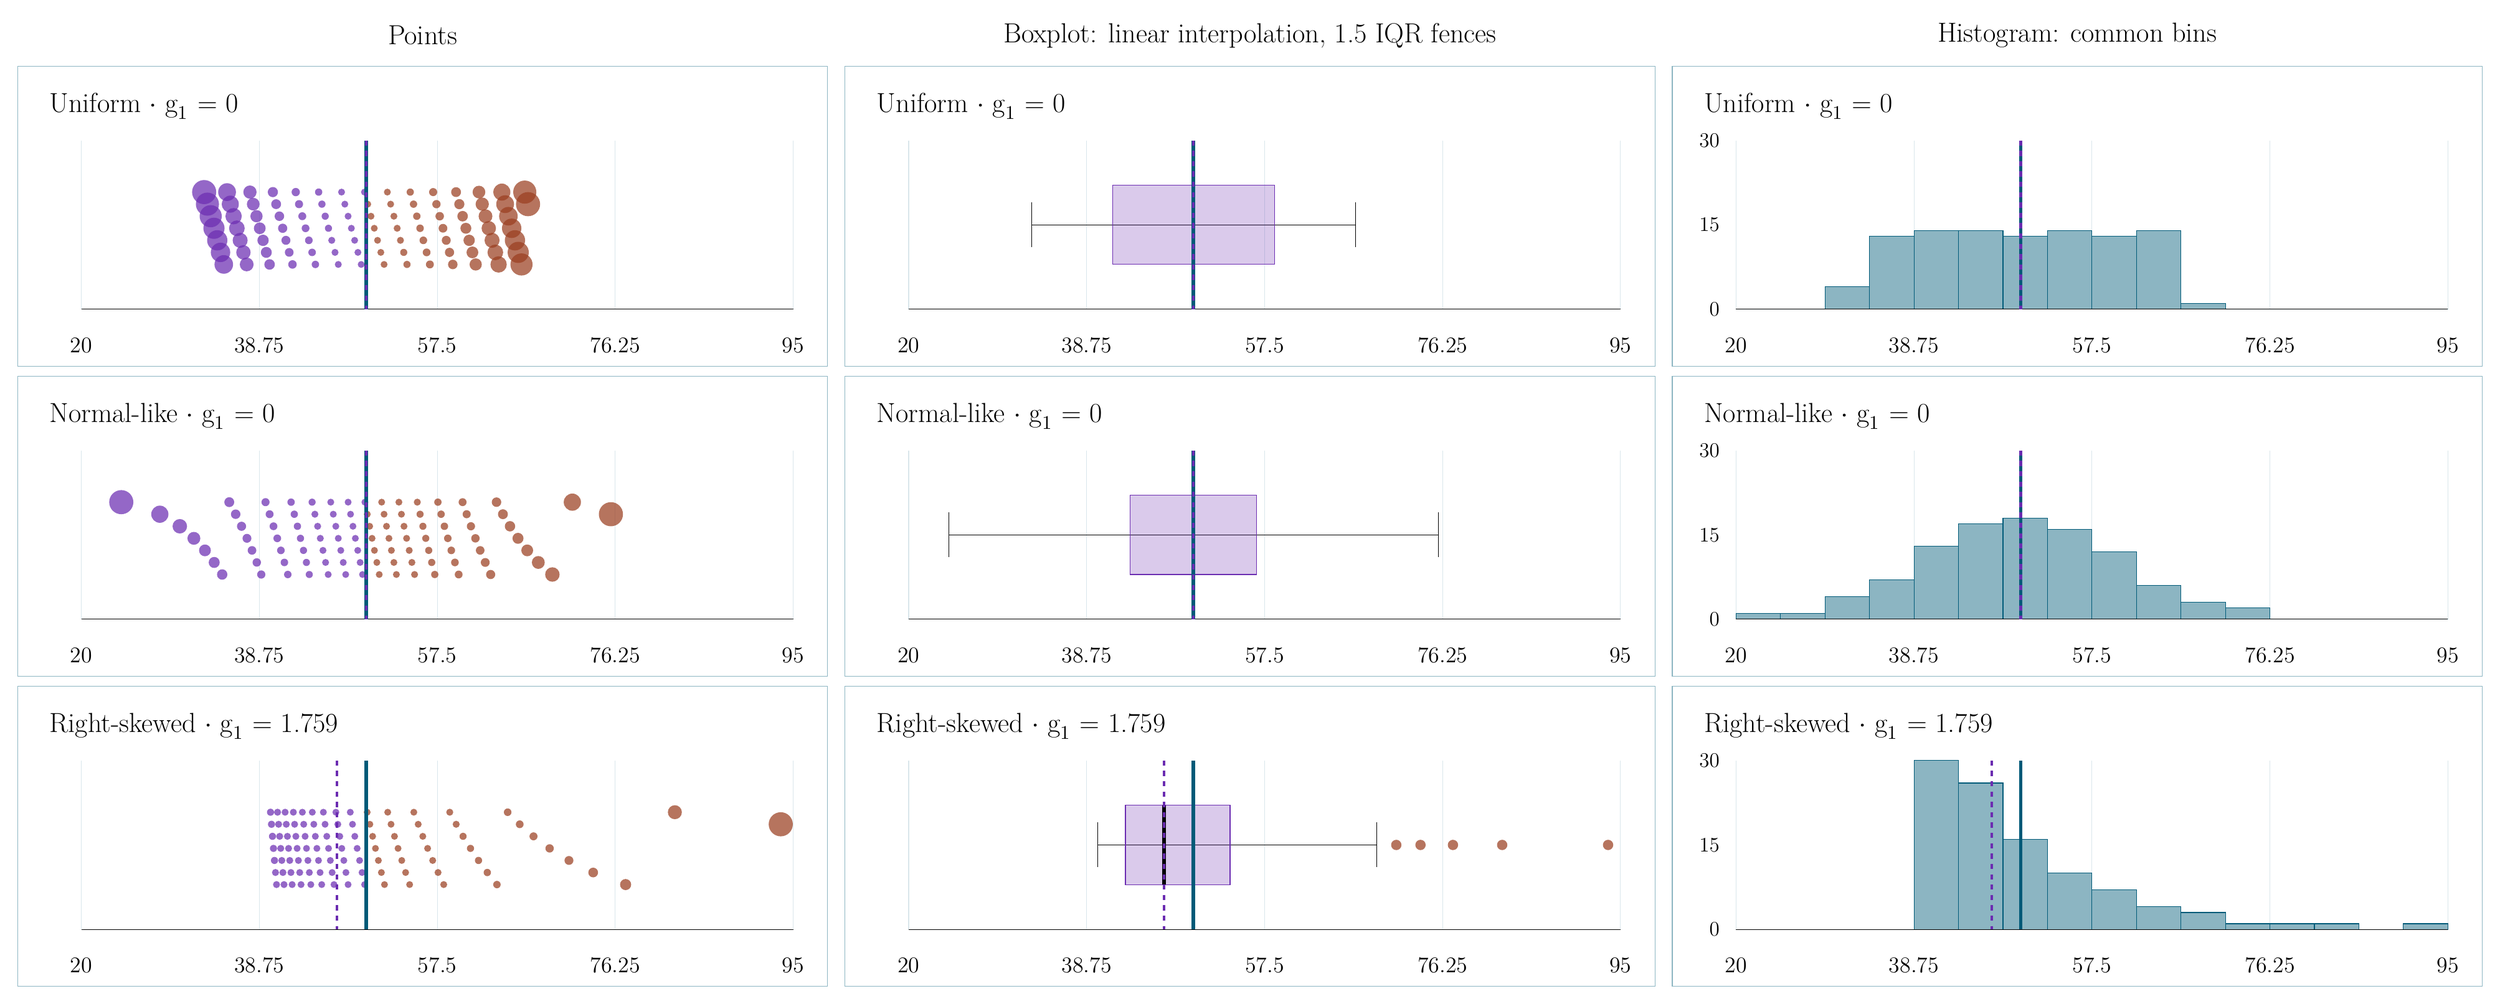
\begin{tikzpicture}[x=1pt,y=-1pt]
\node[anchor=center,font=\fontsize{16}{19}\selectfont] at (240,24) {Points};
\node[anchor=center,font=\fontsize{16}{19}\selectfont] at (720,24) {Boxplot: linear interpolation, 1.5 IQR fences};
\node[anchor=center,font=\fontsize{16}{19}\selectfont] at (1200,24) {Histogram: common bins};
\begin{scope}[shift={(0,40)}]
\path[draw=pcd1!45] (5,2) rectangle (475,176);
\node[anchor=west,font=\fontsize{16}{19}\selectfont] at (20,25) {Uniform \ensuremath{\cdot} g\ensuremath{{}_1} = 0};
\draw[draw=pcd1!15] (42,45) -- (42,143);
\node[anchor=center,font=\fontsize{13}{16}\selectfont] at (42,164) {20};
\draw[draw=pcd1!15] (145.25,45) -- (145.25,143);
\node[anchor=center,font=\fontsize{13}{16}\selectfont] at (145.25,164) {38.75};
\draw[draw=pcd1!15] (248.5,45) -- (248.5,143);
\node[anchor=center,font=\fontsize{13}{16}\selectfont] at (248.5,164) {57.5};
\draw[draw=pcd1!15] (351.75,45) -- (351.75,143);
\node[anchor=center,font=\fontsize{13}{16}\selectfont] at (351.75,164) {76.25};
\draw[draw=pcd1!15] (455,45) -- (455,143);
\node[anchor=center,font=\fontsize{13}{16}\selectfont] at (455,164) {95};
\fill[pcd2,opacity=.72] (113.24412891739694,75) circle[radius=6.999999999999994pt];
\fill[pcd2,opacity=.72] (115.14222732310145,82) circle[radius=6.703050296867961pt];
\fill[pcd2,opacity=.72] (117.04032572881144,89) circle[radius=6.418096895905838pt];
\fill[pcd2,opacity=.72] (118.93842413452143,96) circle[radius=6.144892450677989pt];
\fill[pcd2,opacity=.72] (120.83652254023141,103) circle[radius=5.883189614747904pt];
\fill[pcd2,opacity=.72] (122.7346209459414,110) circle[radius=5.632741041679069pt];
\fill[pcd2,opacity=.72] (124.63271935165137,117) circle[radius=5.393299385034976pt];
\fill[pcd2,opacity=.72] (126.53081775736136,75) circle[radius=5.164617298379113pt];
\fill[pcd2,opacity=.72] (128.42891616306582,82) circle[radius=4.946447435275587pt];
\fill[pcd2,opacity=.72] (130.32701456877584,89) circle[radius=4.738542449286621pt];
\fill[pcd2,opacity=.72] (132.2251129744858,96) circle[radius=4.54065499397635pt];
\fill[pcd2,opacity=.72] (134.1232113801958,103) circle[radius=4.3525377229082665pt];
\fill[pcd2,opacity=.72] (136.02130978590577,110) circle[radius=4.173943289645857pt];
\fill[pcd2,opacity=.72] (137.9194081916158,117) circle[radius=4.0046243477526104pt];
\fill[pcd2,opacity=.72] (139.81750659732575,75) circle[radius=3.844333550792017pt];
\fill[pcd2,opacity=.72] (141.71560500303025,82) circle[radius=3.69282355232799pt];
\fill[pcd2,opacity=.72] (143.61370340874024,89) circle[radius=3.5498470059231435pt];
\fill[pcd2,opacity=.72] (145.51180181445022,96) circle[radius=3.415156565141417pt];
\fill[pcd2,opacity=.72] (147.4099002201602,103) circle[radius=3.288504883546299pt];
\fill[pcd2,opacity=.72] (149.3079986258702,110) circle[radius=3.1696446147012782pt];
\fill[pcd2,opacity=.72] (151.20609703158019,117) circle[radius=3.058328412169844pt];
\fill[pcd2,opacity=.72] (153.10419543729017,75) circle[radius=2.9543089295154847pt];
\fill[pcd2,opacity=.72] (155.00229384299465,82) circle[radius=2.857338820301962pt];
\fill[pcd2,opacity=.72] (156.90039224870463,89) circle[radius=2.7671707380922004pt];
\fill[pcd2,opacity=.72] (158.79849065441462,96) circle[radius=2.683557336449981pt];
\fill[pcd2,opacity=.72] (160.6965890601246,103) circle[radius=2.6062512689387938pt];
\fill[pcd2,opacity=.72] (162.59468746583457,110) circle[radius=2.5350051891221264pt];
\fill[pcd2,opacity=.72] (164.49278587154458,117) circle[radius=2.469571750563468pt];
\fill[pcd2,opacity=.72] (166.39088427725454,75) circle[radius=2.409703606826308pt];
\fill[pcd2,opacity=.72] (168.28898268295902,82) circle[radius=2.3551534114742854pt];
\fill[pcd2,opacity=.72] (170.18708108866903,89) circle[radius=2.3056738180705736pt];
\fill[pcd2,opacity=.72] (172.085179494379,96) circle[radius=2.2610174801788268pt];
\fill[pcd2,opacity=.72] (173.98327790008898,103) circle[radius=2.2209370513625344pt];
\fill[pcd2,opacity=.72] (175.88137630579897,110) circle[radius=2.1851851851851847pt];
\fill[pcd2,opacity=.72] (177.77947471150895,117) circle[radius=2.153514535210267pt];
\fill[pcd2,opacity=.72] (179.67757311721897,75) circle[radius=2.1256777550012695pt];
\fill[pcd2,opacity=.72] (181.57567152292344,82) circle[radius=2.101427498121748pt];
\fill[pcd2,opacity=.72] (183.47376992863343,89) circle[radius=2.08051641813505pt];
\fill[pcd2,opacity=.72] (185.37186833434342,96) circle[radius=2.06269716860474pt];
\fill[pcd2,opacity=.72] (187.2699667400534,103) circle[radius=2.047722403094307pt];
\fill[pcd2,opacity=.72] (189.1680651457634,110) circle[radius=2.03534477516724pt];
\fill[pcd2,opacity=.72] (191.06616355147338,117) circle[radius=2.0253169383870278pt];
\fill[pcd2,opacity=.72] (192.96426195718337,75) circle[radius=2.0173915463171586pt];
\fill[pcd2,opacity=.72] (194.8623603628878,82) circle[radius=2.0113212525211375pt];
\fill[pcd2,opacity=.72] (196.76045876859783,89) circle[radius=2.0068587105624176pt];
\fill[pcd2,opacity=.72] (198.65855717430782,96) circle[radius=2.0037565740045093pt];
\fill[pcd2,opacity=.72] (200.55665558001778,103) circle[radius=2.0017674964109005pt];
\fill[pcd2,opacity=.72] (202.4547539857278,110) circle[radius=2.00064413134508pt];
\fill[pcd2,opacity=.72] (204.35285239143775,117) circle[radius=2.000139132370537pt];
\fill[pcd2,opacity=.72] (206.25095079714774,75) circle[radius=2.0000051530507608pt];
\fill[pcd4,opacity=.72] (208.14904920285224,82) circle[radius=2.0000051530507608pt];
\fill[pcd4,opacity=.72] (210.04714760856223,89) circle[radius=2.000139132370537pt];
\fill[pcd4,opacity=.72] (211.94524601427224,96) circle[radius=2.00064413134508pt];
\fill[pcd4,opacity=.72] (213.8433444199822,103) circle[radius=2.0017674964109005pt];
\fill[pcd4,opacity=.72] (215.74144282569222,110) circle[radius=2.0037565740045093pt];
\fill[pcd4,opacity=.72] (217.63954123140218,117) circle[radius=2.006858710562418pt];
\fill[pcd4,opacity=.72] (219.53763963711216,75) circle[radius=2.0113212525211375pt];
\fill[pcd4,opacity=.72] (221.43573804281664,82) circle[radius=2.017391546317159pt];
\fill[pcd4,opacity=.72] (223.33383644852663,89) circle[radius=2.0253169383870278pt];
\fill[pcd4,opacity=.72] (225.2319348542366,96) circle[radius=2.0353447751672404pt];
\fill[pcd4,opacity=.72] (227.13003325994657,103) circle[radius=2.0477224030943075pt];
\fill[pcd4,opacity=.72] (229.0281316656566,110) circle[radius=2.062697168604741pt];
\fill[pcd4,opacity=.72] (230.92623007136655,117) circle[radius=2.080516418135051pt];
\fill[pcd4,opacity=.72] (232.82432847707656,75) circle[radius=2.101427498121749pt];
\fill[pcd4,opacity=.72] (234.722426882781,82) circle[radius=2.125677755001271pt];
\fill[pcd4,opacity=.72] (236.62052528849105,89) circle[radius=2.1535145352102685pt];
\fill[pcd4,opacity=.72] (238.51862369420104,96) circle[radius=2.185185185185186pt];
\fill[pcd4,opacity=.72] (240.416722099911,103) circle[radius=2.2209370513625357pt];
\fill[pcd4,opacity=.72] (242.31482050562101,110) circle[radius=2.2610174801788285pt];
\fill[pcd4,opacity=.72] (244.21291891133097,117) circle[radius=2.3056738180705754pt];
\fill[pcd4,opacity=.72] (246.11101731704096,75) circle[radius=2.3551534114742876pt];
\fill[pcd4,opacity=.72] (248.00911572274543,82) circle[radius=2.4097036068263105pt];
\fill[pcd4,opacity=.72] (249.90721412845545,89) circle[radius=2.4695717505634707pt];
\fill[pcd4,opacity=.72] (251.8053125341654,96) circle[radius=2.5350051891221295pt];
\fill[pcd4,opacity=.72] (253.7034109398754,103) circle[radius=2.606251268938797pt];
\fill[pcd4,opacity=.72] (255.6015093455854,110) circle[radius=2.6835573364499847pt];
\fill[pcd4,opacity=.72] (257.49960775129534,117) circle[radius=2.767170738092204pt];
\fill[pcd4,opacity=.72] (259.39770615700536,75) circle[radius=2.8573388203019654pt];
\fill[pcd4,opacity=.72] (261.2958045627098,82) circle[radius=2.9543089295154887pt];
\fill[pcd4,opacity=.72] (263.1939029684198,89) circle[radius=3.0583284121698484pt];
\fill[pcd4,opacity=.72] (265.09200137412984,96) circle[radius=3.1696446147012827pt];
\fill[pcd4,opacity=.72] (266.9900997798398,103) circle[radius=3.288504883546304pt];
\fill[pcd4,opacity=.72] (268.88819818554975,110) circle[radius=3.415156565141422pt];
\fill[pcd4,opacity=.72] (270.78629659125977,117) circle[radius=3.549847005923149pt];
\fill[pcd4,opacity=.72] (272.6843949969698,75) circle[radius=3.692823552327996pt];
\fill[pcd4,opacity=.72] (274.58249340267423,82) circle[radius=3.8443335507920233pt];
\fill[pcd4,opacity=.72] (276.48059180838425,89) circle[radius=4.0046243477526176pt];
\fill[pcd4,opacity=.72] (278.3786902140942,96) circle[radius=4.173943289645864pt];
\fill[pcd4,opacity=.72] (280.27678861980417,103) circle[radius=4.352537722908274pt];
\fill[pcd4,opacity=.72] (282.1748870255142,110) circle[radius=4.540654993976359pt];
\fill[pcd4,opacity=.72] (284.0729854312242,117) circle[radius=4.738542449286629pt];
\fill[pcd4,opacity=.72] (285.97108383693416,75) circle[radius=4.946447435275596pt];
\fill[pcd4,opacity=.72] (287.86918224263866,82) circle[radius=5.164617298379127pt];
\fill[pcd4,opacity=.72] (289.7672806483487,89) circle[radius=5.393299385034991pt];
\fill[pcd4,opacity=.72] (291.6653790540587,96) circle[radius=5.632741041679084pt];
\fill[pcd4,opacity=.72] (293.5634774597686,103) circle[radius=5.883189614747919pt];
\fill[pcd4,opacity=.72] (295.4615758654786,110) circle[radius=6.144892450678006pt];
\fill[pcd4,opacity=.72] (297.3596742711886,117) circle[radius=6.418096895905855pt];
\fill[pcd4,opacity=.72] (299.25777267689307,75) circle[radius=6.703050296867127pt];
\fill[pcd4,opacity=.72] (301.155871082603,82) circle[radius=7pt];
\draw[draw=black] (42,143) -- (455,143);
\draw[draw=pcd1,line width=2pt] (207.19999999999996,45) -- (207.19999999999996,143);
\draw[draw=pcd2,dashed,line width=1.5pt] (207.20000000000002,45) -- (207.20000000000002,143);
\end{scope}
\begin{scope}[shift={(480,40)}]
\path[draw=pcd1!45] (5,2) rectangle (475,176);
\node[anchor=west,font=\fontsize{16}{19}\selectfont] at (20,25) {Uniform \ensuremath{\cdot} g\ensuremath{{}_1} = 0};
\draw[draw=pcd1!15] (42,45) -- (42,143);
\node[anchor=center,font=\fontsize{13}{16}\selectfont] at (42,164) {20};
\draw[draw=pcd1!15] (145.25,45) -- (145.25,143);
\node[anchor=center,font=\fontsize{13}{16}\selectfont] at (145.25,164) {38.75};
\draw[draw=pcd1!15] (248.5,45) -- (248.5,143);
\node[anchor=center,font=\fontsize{13}{16}\selectfont] at (248.5,164) {57.5};
\draw[draw=pcd1!15] (351.75,45) -- (351.75,143);
\node[anchor=center,font=\fontsize{13}{16}\selectfont] at (351.75,164) {76.25};
\draw[draw=pcd1!15] (455,45) -- (455,143);
\node[anchor=center,font=\fontsize{13}{16}\selectfont] at (455,164) {95};
\draw[draw=black] (113.24412891739694,94) -- (301.155871082603,94);
\path[fill=pcd2,fill opacity=.25,draw=pcd2] (160.22206445869708,71) rectangle (254.1779355413029,117);
\draw[draw=black,line width=2pt] (207.20000000000002,71) -- (207.20000000000002,117);
\draw[draw=black] (113.24412891739694,81) -- (113.24412891739694,107);
\draw[draw=black] (301.155871082603,81) -- (301.155871082603,107);
\draw[draw=black] (42,143) -- (455,143);
\draw[draw=pcd1,line width=2pt] (207.19999999999996,45) -- (207.19999999999996,143);
\draw[draw=pcd2,dashed,line width=1.5pt] (207.20000000000002,45) -- (207.20000000000002,143);
\end{scope}
\begin{scope}[shift={(960,40)}]
\path[draw=pcd1!45] (5,2) rectangle (475,176);
\node[anchor=west,font=\fontsize{16}{19}\selectfont] at (20,25) {Uniform \ensuremath{\cdot} g\ensuremath{{}_1} = 0};
\draw[draw=pcd1!15] (42,45) -- (42,143);
\node[anchor=center,font=\fontsize{13}{16}\selectfont] at (42,164) {20};
\draw[draw=pcd1!15] (145.25,45) -- (145.25,143);
\node[anchor=center,font=\fontsize{13}{16}\selectfont] at (145.25,164) {38.75};
\draw[draw=pcd1!15] (248.5,45) -- (248.5,143);
\node[anchor=center,font=\fontsize{13}{16}\selectfont] at (248.5,164) {57.5};
\draw[draw=pcd1!15] (351.75,45) -- (351.75,143);
\node[anchor=center,font=\fontsize{13}{16}\selectfont] at (351.75,164) {76.25};
\draw[draw=pcd1!15] (455,45) -- (455,143);
\node[anchor=center,font=\fontsize{13}{16}\selectfont] at (455,164) {95};
\path[fill=pcd1,fill opacity=.45,draw=pcd1] (42,143) rectangle (67.8125,143);
\path[fill=pcd1,fill opacity=.45,draw=pcd1] (67.8125,143) rectangle (93.625,143);
\path[fill=pcd1,fill opacity=.45,draw=pcd1] (93.625,129.93333333333334) rectangle (119.4375,143);
\path[fill=pcd1,fill opacity=.45,draw=pcd1] (119.4375,100.53333333333333) rectangle (145.25,143);
\path[fill=pcd1,fill opacity=.45,draw=pcd1] (145.25,97.26666666666667) rectangle (171.0625,143);
\path[fill=pcd1,fill opacity=.45,draw=pcd1] (171.0625,97.26666666666667) rectangle (196.875,143);
\path[fill=pcd1,fill opacity=.45,draw=pcd1] (196.875,100.53333333333333) rectangle (222.6875,143);
\path[fill=pcd1,fill opacity=.45,draw=pcd1] (222.6875,97.26666666666667) rectangle (248.5,143);
\path[fill=pcd1,fill opacity=.45,draw=pcd1] (248.5,100.53333333333333) rectangle (274.3125,143);
\path[fill=pcd1,fill opacity=.45,draw=pcd1] (274.3125,97.26666666666667) rectangle (300.125,143);
\path[fill=pcd1,fill opacity=.45,draw=pcd1] (300.125,139.73333333333332) rectangle (325.9375,143);
\path[fill=pcd1,fill opacity=.45,draw=pcd1] (325.9375,143) rectangle (351.75,143);
\path[fill=pcd1,fill opacity=.45,draw=pcd1] (351.75,143) rectangle (377.5625,143);
\path[fill=pcd1,fill opacity=.45,draw=pcd1] (377.5625,143) rectangle (403.375,143);
\path[fill=pcd1,fill opacity=.45,draw=pcd1] (403.375,143) rectangle (429.1875,143);
\path[fill=pcd1,fill opacity=.45,draw=pcd1] (429.1875,143) rectangle (455,143);
\node[anchor=east,font=\fontsize{12}{15}\selectfont] at (36,143) {0};
\node[anchor=east,font=\fontsize{12}{15}\selectfont] at (36,94) {15};
\node[anchor=east,font=\fontsize{12}{15}\selectfont] at (36,45) {30};
\draw[draw=black] (42,143) -- (455,143);
\draw[draw=pcd1,line width=2pt] (207.19999999999996,45) -- (207.19999999999996,143);
\draw[draw=pcd2,dashed,line width=1.5pt] (207.20000000000002,45) -- (207.20000000000002,143);
\end{scope}
\begin{scope}[shift={(0,220)}]
\path[draw=pcd1!45] (5,2) rectangle (475,176);
\node[anchor=west,font=\fontsize{16}{19}\selectfont] at (20,25) {Normal-like \ensuremath{\cdot} g\ensuremath{{}_1} = 0};
\draw[draw=pcd1!15] (42,45) -- (42,143);
\node[anchor=center,font=\fontsize{13}{16}\selectfont] at (42,164) {20};
\draw[draw=pcd1!15] (145.25,45) -- (145.25,143);
\node[anchor=center,font=\fontsize{13}{16}\selectfont] at (145.25,164) {38.75};
\draw[draw=pcd1!15] (248.5,45) -- (248.5,143);
\node[anchor=center,font=\fontsize{13}{16}\selectfont] at (248.5,164) {57.5};
\draw[draw=pcd1!15] (351.75,45) -- (351.75,143);
\node[anchor=center,font=\fontsize{13}{16}\selectfont] at (351.75,164) {76.25};
\draw[draw=pcd1!15] (455,45) -- (455,143);
\node[anchor=center,font=\fontsize{13}{16}\selectfont] at (455,164) {95};
\fill[pcd2,opacity=.72] (65.16454133626237,75) circle[radius=7pt];
\fill[pcd2,opacity=.72] (87.53765215058463,82) circle[radius=4.98986947549751pt];
\fill[pcd2,opacity=.72] (99.12436660107437,89) circle[radius=4.20273898737333pt];
\fill[pcd2,opacity=.72] (107.28826938338861,96) circle[radius=3.7403200159000356pt];
\fill[pcd2,opacity=.72] (113.7129855211349,103) circle[radius=3.425717703713766pt];
\fill[pcd2,opacity=.72] (119.0730051912103,110) circle[radius=3.194281079772998pt];
\fill[pcd2,opacity=.72] (123.70993496528129,117) circle[radius=3.015509681704306pt];
\fill[pcd2,opacity=.72] (127.82187022489454,75) circle[radius=2.8727347265408727pt];
\fill[pcd2,opacity=.72] (131.53442809166978,82) circle[radius=2.755917895949483pt];
\fill[pcd2,opacity=.72] (134.93251509506104,89) circle[radius=2.6585799297629356pt];
\fill[pcd2,opacity=.72] (138.07634270918393,96) circle[radius=2.576314830035689pt];
\fill[pcd2,opacity=.72] (141.01024094780104,103) circle[radius=2.5060018103603547pt];
\fill[pcd2,opacity=.72] (143.76784568754908,110) circle[radius=2.445356765639766pt];
\fill[pcd2,opacity=.72] (146.37531884246346,117) circle[radius=2.3926622884428093pt];
\fill[pcd2,opacity=.72] (148.85343600881788,75) circle[radius=2.3465975809461734pt];
\fill[pcd2,opacity=.72] (151.21898956004614,82) circle[radius=2.30612716491815pt];
\fill[pcd2,opacity=.72] (153.48576081178732,89) circle[radius=2.270425696179122pt];
\fill[pcd2,opacity=.72] (155.66521140319736,96) circle[radius=2.2388257590656693pt];
\fill[pcd2,opacity=.72] (157.7669862283159,103) circle[radius=2.210780745698171pt];
\fill[pcd2,opacity=.72] (159.7992865920125,110) circle[radius=2.1858379065493603pt];
\fill[pcd2,opacity=.72] (161.76915195659856,117) circle[radius=2.1636184225865835pt];
\fill[pcd2,opacity=.72] (163.68267600478754,75) circle[radius=2.143802426627175pt];
\fill[pcd2,opacity=.72] (165.54517465782482,82) circle[radius=2.1261175785346222pt];
\fill[pcd2,opacity=.72] (167.36131838621117,89) circle[radius=2.110330235123875pt];
\fill[pcd2,opacity=.72] (169.1352375982878,96) circle[radius=2.0962385431540587pt];
\fill[pcd2,opacity=.72] (170.87060746462737,103) circle[radius=2.083666977155453pt];
\fill[pcd2,opacity=.72] (172.5707168478382,110) circle[radius=2.072461976298883pt];
\fill[pcd2,opacity=.72] (174.2385248135968,117) circle[radius=2.062488426785014pt];
\fill[pcd2,opacity=.72] (175.87670734235186,75) circle[radius=2.053626801488994pt];
\fill[pcd2,opacity=.72] (177.4876962383739,82) circle[radius=2.0457708154016028pt];
\fill[pcd2,opacity=.72] (179.07371177394688,89) circle[radius=2.038825489415549pt];
\fill[pcd2,opacity=.72] (180.63679026512506,96) circle[radius=2.032705540006251pt];
\fill[pcd2,opacity=.72] (182.17880751793538,103) circle[radius=2.027334030943675pt];
\fill[pcd2,opacity=.72] (183.7014988885424,110) circle[radius=2.022641237127984pt];
\fill[pcd2,opacity=.72] (185.20647655075038,117) circle[radius=2.018563681223438pt];
\fill[pcd2,opacity=.72] (186.69524444809016,75) circle[radius=2.015043311857634pt];
\fill[pcd2,opacity=.72] (188.16921131713553,82) circle[radius=2.0120267983931863pt];
\fill[pcd2,opacity=.72] (189.62970209763023,89) circle[radius=2.009464922126561pt];
\fill[pcd2,opacity=.72] (191.07796798874614,96) circle[radius=2.007312047561401pt];
\fill[pcd2,opacity=.72] (192.51519536587472,103) circle[radius=2.005525660389674pt];
\fill[pcd2,opacity=.72] (193.94251373685682,110) circle[radius=2.0040659611773566pt];
\fill[pcd2,opacity=.72] (195.36100288752172,117) circle[radius=2.0028955056327296pt];
\fill[pcd2,opacity=.72] (196.77169934342442,75) circle[radius=2.0019788838376207pt];
\fill[pcd2,opacity=.72] (198.17560225582272,82) circle[radius=2.0012824320260987pt];
\fill[pcd2,opacity=.72] (199.57367880477972,89) circle[radius=2.0007739714614328pt];
\fill[pcd2,opacity=.72] (200.96686920014255,96) circle[radius=2.0004225697375224pt];
\fill[pcd2,opacity=.72] (202.3560913510083,103) circle[radius=2.0001983204516653pt];
\fill[pcd2,opacity=.72] (203.74224526671262,110) circle[radius=2.0000721376887567pt];
\fill[pcd2,opacity=.72] (205.1262172457786,117) circle[radius=2.0000155621445788pt];
\fill[pcd2,opacity=.72] (206.50888390477604,75) circle[radius=2.0000005760135395pt];
\fill[pcd4,opacity=.72] (207.89111609522396,82) circle[radius=2.0000005760135395pt];
\fill[pcd4,opacity=.72] (209.27378275422137,89) circle[radius=2.0000155621445788pt];
\fill[pcd4,opacity=.72] (210.6577547332874,96) circle[radius=2.0000721376887567pt];
\fill[pcd4,opacity=.72] (212.0439086489917,103) circle[radius=2.0001983204516653pt];
\fill[pcd4,opacity=.72] (213.43313079985745,110) circle[radius=2.0004225697375224pt];
\fill[pcd4,opacity=.72] (214.8263211952203,117) circle[radius=2.0007739714614328pt];
\fill[pcd4,opacity=.72] (216.22439774417728,75) circle[radius=2.0012824320260987pt];
\fill[pcd4,opacity=.72] (217.62830065657556,82) circle[radius=2.0019788838376207pt];
\fill[pcd4,opacity=.72] (219.03899711247826,89) circle[radius=2.0028955056327296pt];
\fill[pcd4,opacity=.72] (220.45748626314318,96) circle[radius=2.0040659611773566pt];
\fill[pcd4,opacity=.72] (221.8848046341253,103) circle[radius=2.005525660389674pt];
\fill[pcd4,opacity=.72] (223.32203201125384,110) circle[radius=2.007312047561401pt];
\fill[pcd4,opacity=.72] (224.77029790236978,117) circle[radius=2.009464922126561pt];
\fill[pcd4,opacity=.72] (226.23078868286447,75) circle[radius=2.0120267983931863pt];
\fill[pcd4,opacity=.72] (227.70475555190984,82) circle[radius=2.015043311857634pt];
\fill[pcd4,opacity=.72] (229.1935234492496,89) circle[radius=2.018563681223438pt];
\fill[pcd4,opacity=.72] (230.6985011114576,96) circle[radius=2.022641237127984pt];
\fill[pcd4,opacity=.72] (232.22119248206462,103) circle[radius=2.027334030943675pt];
\fill[pcd4,opacity=.72] (233.76320973487495,110) circle[radius=2.032705540006251pt];
\fill[pcd4,opacity=.72] (235.3262882260531,117) circle[radius=2.038825489415549pt];
\fill[pcd4,opacity=.72] (236.91230376162608,75) circle[radius=2.0457708154016028pt];
\fill[pcd4,opacity=.72] (238.52329265764814,82) circle[radius=2.053626801488994pt];
\fill[pcd4,opacity=.72] (240.16147518640324,89) circle[radius=2.062488426785014pt];
\fill[pcd4,opacity=.72] (241.8292831521618,96) circle[radius=2.072461976298883pt];
\fill[pcd4,opacity=.72] (243.52939253537264,103) circle[radius=2.083666977155453pt];
\fill[pcd4,opacity=.72] (245.2647624017122,110) circle[radius=2.0962385431540587pt];
\fill[pcd4,opacity=.72] (247.03868161378887,117) circle[radius=2.110330235123875pt];
\fill[pcd4,opacity=.72] (248.8548253421752,75) circle[radius=2.1261175785346222pt];
\fill[pcd4,opacity=.72] (250.71732399521247,82) circle[radius=2.143802426627175pt];
\fill[pcd4,opacity=.72] (252.63084804340141,89) circle[radius=2.1636184225865835pt];
\fill[pcd4,opacity=.72] (254.60071340798754,96) circle[radius=2.1858379065493603pt];
\fill[pcd4,opacity=.72] (256.6330137716841,103) circle[radius=2.210780745698171pt];
\fill[pcd4,opacity=.72] (258.7347885968027,110) circle[radius=2.2388257590656693pt];
\fill[pcd4,opacity=.72] (260.9142391882127,117) circle[radius=2.270425696179122pt];
\fill[pcd4,opacity=.72] (263.18101043995387,75) circle[radius=2.30612716491815pt];
\fill[pcd4,opacity=.72] (265.5465639911821,82) circle[radius=2.3465975809461734pt];
\fill[pcd4,opacity=.72] (268.0246811575365,89) circle[radius=2.3926622884428093pt];
\fill[pcd4,opacity=.72] (270.63215431245095,96) circle[radius=2.445356765639766pt];
\fill[pcd4,opacity=.72] (273.389759052199,103) circle[radius=2.5060018103603547pt];
\fill[pcd4,opacity=.72] (276.3236572908161,110) circle[radius=2.576314830035689pt];
\fill[pcd4,opacity=.72] (279.46748490493894,117) circle[radius=2.6585799297629356pt];
\fill[pcd4,opacity=.72] (282.86557190833025,75) circle[radius=2.755917895949483pt];
\fill[pcd4,opacity=.72] (286.5781297751055,82) circle[radius=2.872734726540874pt];
\fill[pcd4,opacity=.72] (290.6900650347187,89) circle[radius=3.015509681704306pt];
\fill[pcd4,opacity=.72] (295.3269948087898,96) circle[radius=3.1942810797729995pt];
\fill[pcd4,opacity=.72] (300.6870144788651,103) circle[radius=3.4257177037137643pt];
\fill[pcd4,opacity=.72] (307.1117306166114,110) circle[radius=3.7403200159000356pt];
\fill[pcd4,opacity=.72] (315.27563339892566,117) circle[radius=4.202738987373332pt];
\fill[pcd4,opacity=.72] (326.86234784941536,75) circle[radius=4.989869475497512pt];
\fill[pcd4,opacity=.72] (349.2354586637376,82) circle[radius=6.9999999999999964pt];
\draw[draw=black] (42,143) -- (455,143);
\draw[draw=pcd1,line width=2pt] (207.20000000000002,45) -- (207.20000000000002,143);
\draw[draw=pcd2,dashed,line width=1.5pt] (207.20000000000002,45) -- (207.20000000000002,143);
\end{scope}
\begin{scope}[shift={(480,220)}]
\path[draw=pcd1!45] (5,2) rectangle (475,176);
\node[anchor=west,font=\fontsize{16}{19}\selectfont] at (20,25) {Normal-like \ensuremath{\cdot} g\ensuremath{{}_1} = 0};
\draw[draw=pcd1!15] (42,45) -- (42,143);
\node[anchor=center,font=\fontsize{13}{16}\selectfont] at (42,164) {20};
\draw[draw=pcd1!15] (145.25,45) -- (145.25,143);
\node[anchor=center,font=\fontsize{13}{16}\selectfont] at (145.25,164) {38.75};
\draw[draw=pcd1!15] (248.5,45) -- (248.5,143);
\node[anchor=center,font=\fontsize{13}{16}\selectfont] at (248.5,164) {57.5};
\draw[draw=pcd1!15] (351.75,45) -- (351.75,143);
\node[anchor=center,font=\fontsize{13}{16}\selectfont] at (351.75,164) {76.25};
\draw[draw=pcd1!15] (455,45) -- (455,143);
\node[anchor=center,font=\fontsize{13}{16}\selectfont] at (455,164) {95};
\draw[draw=black] (65.16454133626237,94) -- (349.2354586637376,94);
\path[fill=pcd2,fill opacity=.25,draw=pcd2] (170.43676499804246,71) rectangle (243.96323500195754,117);
\draw[draw=black,line width=2pt] (207.20000000000002,71) -- (207.20000000000002,117);
\draw[draw=black] (65.16454133626237,81) -- (65.16454133626237,107);
\draw[draw=black] (349.2354586637376,81) -- (349.2354586637376,107);
\draw[draw=black] (42,143) -- (455,143);
\draw[draw=pcd1,line width=2pt] (207.20000000000002,45) -- (207.20000000000002,143);
\draw[draw=pcd2,dashed,line width=1.5pt] (207.20000000000002,45) -- (207.20000000000002,143);
\end{scope}
\begin{scope}[shift={(960,220)}]
\path[draw=pcd1!45] (5,2) rectangle (475,176);
\node[anchor=west,font=\fontsize{16}{19}\selectfont] at (20,25) {Normal-like \ensuremath{\cdot} g\ensuremath{{}_1} = 0};
\draw[draw=pcd1!15] (42,45) -- (42,143);
\node[anchor=center,font=\fontsize{13}{16}\selectfont] at (42,164) {20};
\draw[draw=pcd1!15] (145.25,45) -- (145.25,143);
\node[anchor=center,font=\fontsize{13}{16}\selectfont] at (145.25,164) {38.75};
\draw[draw=pcd1!15] (248.5,45) -- (248.5,143);
\node[anchor=center,font=\fontsize{13}{16}\selectfont] at (248.5,164) {57.5};
\draw[draw=pcd1!15] (351.75,45) -- (351.75,143);
\node[anchor=center,font=\fontsize{13}{16}\selectfont] at (351.75,164) {76.25};
\draw[draw=pcd1!15] (455,45) -- (455,143);
\node[anchor=center,font=\fontsize{13}{16}\selectfont] at (455,164) {95};
\path[fill=pcd1,fill opacity=.45,draw=pcd1] (42,139.73333333333332) rectangle (67.8125,143);
\path[fill=pcd1,fill opacity=.45,draw=pcd1] (67.8125,139.73333333333332) rectangle (93.625,143);
\path[fill=pcd1,fill opacity=.45,draw=pcd1] (93.625,129.93333333333334) rectangle (119.4375,143);
\path[fill=pcd1,fill opacity=.45,draw=pcd1] (119.4375,120.13333333333333) rectangle (145.25,143);
\path[fill=pcd1,fill opacity=.45,draw=pcd1] (145.25,100.53333333333333) rectangle (171.0625,143);
\path[fill=pcd1,fill opacity=.45,draw=pcd1] (171.0625,87.46666666666667) rectangle (196.875,143);
\path[fill=pcd1,fill opacity=.45,draw=pcd1] (196.875,84.2) rectangle (222.6875,143);
\path[fill=pcd1,fill opacity=.45,draw=pcd1] (222.6875,90.73333333333333) rectangle (248.5,143);
\path[fill=pcd1,fill opacity=.45,draw=pcd1] (248.5,103.8) rectangle (274.3125,143);
\path[fill=pcd1,fill opacity=.45,draw=pcd1] (274.3125,123.4) rectangle (300.125,143);
\path[fill=pcd1,fill opacity=.45,draw=pcd1] (300.125,133.2) rectangle (325.9375,143);
\path[fill=pcd1,fill opacity=.45,draw=pcd1] (325.9375,136.46666666666667) rectangle (351.75,143);
\path[fill=pcd1,fill opacity=.45,draw=pcd1] (351.75,143) rectangle (377.5625,143);
\path[fill=pcd1,fill opacity=.45,draw=pcd1] (377.5625,143) rectangle (403.375,143);
\path[fill=pcd1,fill opacity=.45,draw=pcd1] (403.375,143) rectangle (429.1875,143);
\path[fill=pcd1,fill opacity=.45,draw=pcd1] (429.1875,143) rectangle (455,143);
\node[anchor=east,font=\fontsize{12}{15}\selectfont] at (36,143) {0};
\node[anchor=east,font=\fontsize{12}{15}\selectfont] at (36,94) {15};
\node[anchor=east,font=\fontsize{12}{15}\selectfont] at (36,45) {30};
\draw[draw=black] (42,143) -- (455,143);
\draw[draw=pcd1,line width=2pt] (207.20000000000002,45) -- (207.20000000000002,143);
\draw[draw=pcd2,dashed,line width=1.5pt] (207.20000000000002,45) -- (207.20000000000002,143);
\end{scope}
\begin{scope}[shift={(0,400)}]
\path[draw=pcd1!45] (5,2) rectangle (475,176);
\node[anchor=west,font=\fontsize{16}{19}\selectfont] at (20,25) {Right-skewed \ensuremath{\cdot} g\ensuremath{{}_1} = 1.759};
\draw[draw=pcd1!15] (42,45) -- (42,143);
\node[anchor=center,font=\fontsize{13}{16}\selectfont] at (42,164) {20};
\draw[draw=pcd1!15] (145.25,45) -- (145.25,143);
\node[anchor=center,font=\fontsize{13}{16}\selectfont] at (145.25,164) {38.75};
\draw[draw=pcd1!15] (248.5,45) -- (248.5,143);
\node[anchor=center,font=\fontsize{13}{16}\selectfont] at (248.5,164) {57.5};
\draw[draw=pcd1!15] (351.75,45) -- (351.75,143);
\node[anchor=center,font=\fontsize{13}{16}\selectfont] at (351.75,164) {76.25};
\draw[draw=pcd1!15] (455,45) -- (455,143);
\node[anchor=center,font=\fontsize{13}{16}\selectfont] at (455,164) {95};
\fill[pcd2,opacity=.72] (151.74905333266133,75) circle[radius=2.0612262855926002pt];
\fill[pcd2,opacity=.72] (152.31395571301317,82) circle[radius=2.0593740690745412pt];
\fill[pcd2,opacity=.72] (152.8846225028966,89) circle[radius=2.05754126762299pt];
\fill[pcd2,opacity=.72] (153.4611725592456,96) circle[radius=2.0557282719551453pt];
\fill[pcd2,opacity=.72] (154.04372845340623,103) circle[radius=2.0539354805170573pt];
\fill[pcd2,opacity=.72] (154.63241662752557,110) circle[radius=2.052163299575772pt];
\fill[pcd2,opacity=.72] (155.22736755930603,117) circle[radius=2.0504121433033062pt];
\fill[pcd2,opacity=.72] (155.8287159355586,75) circle[radius=2.0486824338514427pt];
\fill[pcd2,opacity=.72] (156.4366008352228,82) circle[radius=2.0469746014155414pt];
\fill[pcd2,opacity=.72] (157.0511659224521,89) circle[radius=2.045289084285776pt];
\fill[pcd2,opacity=.72] (157.67255965038294,96) circle[radius=2.043626328884023pt];
\fill[pcd2,opacity=.72] (158.3009354764065,103) circle[radius=2.0419867897840267pt];
\fill[pcd2,opacity=.72] (158.93645208964392,110) circle[radius=2.0403709297126706pt];
\fill[pcd2,opacity=.72] (159.5792736514773,117) circle[radius=2.0387792195296592pt];
\fill[pcd2,opacity=.72] (160.22957005010642,75) circle[radius=2.037212138182457pt];
\fill[pcd2,opacity=.72] (160.88751717007247,82) circle[radius=2.035670172633251pt];
\fill[pcd2,opacity=.72] (161.55329717777346,89) circle[radius=2.034153817754263pt];
\fill[pcd2,opacity=.72] (162.22709882426457,96) circle[radius=2.0326635761868523pt];
\fill[pcd2,opacity=.72] (162.90911776645657,103) circle[radius=2.031199958160001pt];
\fill[pcd2,opacity=.72] (163.59955690818776,110) circle[radius=2.029763481262582pt];
\fill[pcd2,opacity=.72] (164.2986267625626,117) circle[radius=2.0283546701636026pt];
\fill[pcd2,opacity=.72] (165.00654583728073,75) circle[radius=2.0269740562734397pt];
\fill[pcd2,opacity=.72] (165.7235410446304,82) circle[radius=2.025622177338648pt];
\fill[pcd2,opacity=.72] (166.44984813813954,89) circle[radius=2.02429957696162pt];
\fill[pcd2,opacity=.72] (167.1857121779055,96) circle[radius=2.0230068040355995pt];
\fill[pcd2,opacity=.72] (167.93138802701577,103) circle[radius=2.0217444120839256pt];
\fill[pcd2,opacity=.72] (168.68714088144333,110) circle[radius=2.020512958491446pt];
\fill[pcd2,opacity=.72] (169.4532468363193,117) circle[radius=2.0193130036139344pt];
\fill[pcd2,opacity=.72] (170.229993491435,75) circle[radius=2.01814510975008pt];
\fill[pcd2,opacity=.72] (171.01768059949208,82) circle[radius=2.0170098399579195pt];
\fill[pcd2,opacity=.72] (171.8166207605925,89) circle[radius=2.0159077566957984pt];
\fill[pcd2,opacity=.72] (172.6271401670594,96) circle[radius=2.014839420264868pt];
\fill[pcd2,opacity=.72] (173.44957940309263,103) circle[radius=2.013805387027032pt];
\fill[pcd2,opacity=.72] (174.28429430402963,110) circle[radius=2.0128062073689676pt];
\fill[pcd2,opacity=.72] (175.13165688074383,117) circle[radius=2.011842423378422pt];
\fill[pcd2,opacity=.72] (175.99205631517825,75) circle[radius=2.0109145661944283pt];
\fill[pcd2,opacity=.72] (176.86590003362252,82) circle[radius=2.010023152987729pt];
\fill[pcd2,opacity=.72] (177.753614865211,89) circle[radius=2.0091686835212412pt];
\fill[pcd2,opacity=.72] (178.65564829385775,96) circle[radius=2.0083516362333036pt];
\fill[pcd2,opacity=.72] (179.57246981280298,103) circle[radius=2.0075724637779904pt];
\fill[pcd2,opacity=.72] (180.5045723920573,110) circle[radius=2.0068315879470053pt];
\fill[pcd2,opacity=.72] (181.45247407026855,117) circle[radius=2.006129393886316pt];
\fill[pcd2,opacity=.72] (182.41671968376033,75) circle[radius=2.0054662235075846pt];
\fill[pcd2,opacity=.72] (183.39788274731754,82) circle[radius=2.004842367978821pt];
\fill[pcd2,opacity=.72] (184.3965675029305,89) circle[radius=2.004258059160729pt];
\fill[pcd2,opacity=.72] (185.41341115475836,96) circle[radius=2.003713459834014pt];
\fill[pcd2,opacity=.72] (186.44908631115385,103) circle[radius=2.0032086525378325pt];
\fill[pcd2,opacity=.72] (187.5043036570159,110) circle[radius=2.0027436268103282pt];
\fill[pcd2,opacity=.72] (188.5798148832203,117) circle[radius=2.0023182645872377pt];
\fill[pcd2,opacity=.72] (189.6764159032678,75) circle[radius=2.001932323473468pt];
\fill[pcd2,opacity=.72] (190.79495039163652,82) circle[radius=2.001585417553477pt];
\fill[pcd2,opacity=.72] (191.93631368331717,89) circle[radius=2.001276995347888pt];
\fill[pcd2,opacity=.72] (193.10145707959668,96) circle[radius=2.0010063144539876pt];
\fill[pcd2,opacity=.72] (194.29139261200237,103) circle[radius=2.000772412323978pt];
\fill[pcd2,opacity=.72] (195.50719832418628,110) circle[radius=2.0005740725341097pt];
\fill[pcd2,opacity=.72] (196.75002414084807,117) circle[radius=2.0004097857761582pt];
\fill[pcd2,opacity=.72] (198.02109840369124,75) circle[radius=2.0002777046553435pt];
\fill[pcd2,opacity=.72] (199.32173516762984,82) circle[radius=2.000175591199498pt];
\fill[pcd2,opacity=.72] (200.65334236577635,89) circle[radius=2.0001007557654806pt];
\fill[pcd2,opacity=.72] (202.01743097046457,96) circle[radius=2.0000499857605596pt];
\fill[pcd2,opacity=.72] (203.41562529973626,103) circle[radius=2.0000194622662497pt];
\fill[pcd2,opacity=.72] (204.8496746455543,110) circle[radius=2.0000046622437466pt];
\fill[pcd2,opacity=.72] (206.32146643258295,117) circle[radius=2.0000002434927855pt];
\fill[pcd4,opacity=.72] (207.83304115577005,75) circle[radius=2.0000000910975833pt];
\fill[pcd4,opacity=.72] (209.38660939333695,82) circle[radius=2.0000037542625964pt];
\fill[pcd4,opacity=.72] (210.98457125113228,89) circle[radius=2.00001946529887pt];
\fill[pcd4,opacity=.72] (212.62953866760014,96) circle[radius=2.0000574777566658pt];
\fill[pcd4,opacity=.72] (214.32436109975887,103) circle[radius=2.0001298520436994pt];
\fill[pcd4,opacity=.72] (216.07215522438784,110) circle[radius=2.0002507831844287pt];
\fill[pcd4,opacity=.72] (217.87633943208505,117) circle[radius=2.000436996679235pt];
\fill[pcd4,opacity=.72] (219.74067407326876,75) circle[radius=2.000708228926514pt];
\fill[pcd4,opacity=.72] (221.66930864696866,82) circle[radius=2.001087813290321pt];
\fill[pcd4,opacity=.72] (223.6668374211214,89) circle[radius=2.00160339901079pt];
\fill[pcd4,opacity=.72] (225.73836535942488,96) circle[radius=2.0022878383183382pt];
\fill[pcd4,opacity=.72] (227.8895867350018,103) circle[radius=2.0031802881134504pt];
\fill[pcd4,opacity=.72] (230.12687947830563,110) circle[radius=2.0043275875453084pt];
\fill[pcd4,opacity=.72] (232.45741919635435,117) circle[radius=2.005785993415314pt];
\fill[pcd4,opacity=.72] (234.88931799995487,75) circle[radius=2.0076233839823985pt];
\fill[pcd4,opacity=.72] (237.43179491204052,82) circle[radius=2.0099220821042554pt];
\fill[pcd4,opacity=.72] (240.09538689072,89) circle[radius=2.012782506260101pt];
\fill[pcd4,opacity=.72] (242.89221266713076,96) circle[radius=2.016327941446266pt];
\fill[pcd4,opacity=.72] (245.83630609978727,103) circle[radius=2.0207108447279154pt];
\fill[pcd4,opacity=.72] (248.94404225387817,110) circle[radius=2.0261212840795477pt];
\fill[pcd4,opacity=.72] (252.23468898849328,117) circle[radius=2.0327983897042796pt];
\fill[pcd4,opacity=.72] (255.7311312088646,75) circle[radius=2.041046134262146pt];
\fill[pcd4,opacity=.72] (259.4608370005535,82) circle[radius=2.051255455969766pt];
\fill[pcd4,opacity=.72] (263.4571695673268,89) circle[radius=2.0639358807555754pt];
\fill[pcd4,opacity=.72] (267.76120502944525,96) circle[radius=2.079761725835196pt];
\fill[pcd4,opacity=.72] (272.4243098479891,103) circle[radius=2.0996413253574633pt];
\fill[pcd4,opacity=.72] (277.51189382125017,110) circle[radius=2.1248238015890735pt];
\fill[pcd4,opacity=.72] (283.10904724383096,117) circle[radius=2.1570694199043663pt];
\fill[pcd4,opacity=.72] (289.3293253318585,75) circle[radius=2.1989325199317196pt];
\fill[pcd4,opacity=.72] (296.32905659681717,82) circle[radius=2.254254675130913pt];
\fill[pcd4,opacity=.72] (304.33195126399306,89) circle[radius=2.329076870164828pt];
\fill[pcd4,opacity=.72] (313.67442758535555,96) circle[radius=2.4334579374445253pt];
\fill[pcd4,opacity=.72] (324.89690816418914,103) circle[radius=2.585472069113312pt];
\fill[pcd4,opacity=.72] (338.9516324181069,110) circle[radius=2.8212569027996635pt];
\fill[pcd4,opacity=.72] (357.76879519367947,117) circle[radius=3.2257896335801153pt];
\fill[pcd4,opacity=.72] (386.3366467610514,75) circle[radius=4.064259726474253pt];
\fill[pcd4,opacity=.72] (447.7763853579136,82) circle[radius=7pt];
\draw[draw=black] (42,143) -- (455,143);
\draw[draw=pcd1,line width=2pt] (207.19999999999996,45) -- (207.19999999999996,143);
\draw[draw=pcd2,dashed,line width=1.5pt] (190.23568314745216,45) -- (190.23568314745216,143);
\end{scope}
\begin{scope}[shift={(480,400)}]
\path[draw=pcd1!45] (5,2) rectangle (475,176);
\node[anchor=west,font=\fontsize{16}{19}\selectfont] at (20,25) {Right-skewed \ensuremath{\cdot} g\ensuremath{{}_1} = 1.759};
\draw[draw=pcd1!15] (42,45) -- (42,143);
\node[anchor=center,font=\fontsize{13}{16}\selectfont] at (42,164) {20};
\draw[draw=pcd1!15] (145.25,45) -- (145.25,143);
\node[anchor=center,font=\fontsize{13}{16}\selectfont] at (145.25,164) {38.75};
\draw[draw=pcd1!15] (248.5,45) -- (248.5,143);
\node[anchor=center,font=\fontsize{13}{16}\selectfont] at (248.5,164) {57.5};
\draw[draw=pcd1!15] (351.75,45) -- (351.75,143);
\node[anchor=center,font=\fontsize{13}{16}\selectfont] at (351.75,164) {76.25};
\draw[draw=pcd1!15] (455,45) -- (455,143);
\node[anchor=center,font=\fontsize{13}{16}\selectfont] at (455,164) {95};
\draw[draw=black] (151.74905333266133,94) -- (313.67442758535555,94);
\path[fill=pcd2,fill opacity=.25,draw=pcd2] (167.7449690647382,71) rectangle (228.4489099208277,117);
\draw[draw=black,line width=2pt] (190.23568314745216,71) -- (190.23568314745216,117);
\draw[draw=black] (151.74905333266133,81) -- (151.74905333266133,107);
\draw[draw=black] (313.67442758535555,81) -- (313.67442758535555,107);
\fill[pcd4,opacity=.72] (324.89690816418914,94) circle[radius=3pt];
\fill[pcd4,opacity=.72] (338.9516324181069,94) circle[radius=3pt];
\fill[pcd4,opacity=.72] (357.76879519367947,94) circle[radius=3pt];
\fill[pcd4,opacity=.72] (386.3366467610514,94) circle[radius=3pt];
\fill[pcd4,opacity=.72] (447.7763853579136,94) circle[radius=3pt];
\draw[draw=black] (42,143) -- (455,143);
\draw[draw=pcd1,line width=2pt] (207.19999999999996,45) -- (207.19999999999996,143);
\draw[draw=pcd2,dashed,line width=1.5pt] (190.23568314745216,45) -- (190.23568314745216,143);
\end{scope}
\begin{scope}[shift={(960,400)}]
\path[draw=pcd1!45] (5,2) rectangle (475,176);
\node[anchor=west,font=\fontsize{16}{19}\selectfont] at (20,25) {Right-skewed \ensuremath{\cdot} g\ensuremath{{}_1} = 1.759};
\draw[draw=pcd1!15] (42,45) -- (42,143);
\node[anchor=center,font=\fontsize{13}{16}\selectfont] at (42,164) {20};
\draw[draw=pcd1!15] (145.25,45) -- (145.25,143);
\node[anchor=center,font=\fontsize{13}{16}\selectfont] at (145.25,164) {38.75};
\draw[draw=pcd1!15] (248.5,45) -- (248.5,143);
\node[anchor=center,font=\fontsize{13}{16}\selectfont] at (248.5,164) {57.5};
\draw[draw=pcd1!15] (351.75,45) -- (351.75,143);
\node[anchor=center,font=\fontsize{13}{16}\selectfont] at (351.75,164) {76.25};
\draw[draw=pcd1!15] (455,45) -- (455,143);
\node[anchor=center,font=\fontsize{13}{16}\selectfont] at (455,164) {95};
\path[fill=pcd1,fill opacity=.45,draw=pcd1] (42,143) rectangle (67.8125,143);
\path[fill=pcd1,fill opacity=.45,draw=pcd1] (67.8125,143) rectangle (93.625,143);
\path[fill=pcd1,fill opacity=.45,draw=pcd1] (93.625,143) rectangle (119.4375,143);
\path[fill=pcd1,fill opacity=.45,draw=pcd1] (119.4375,143) rectangle (145.25,143);
\path[fill=pcd1,fill opacity=.45,draw=pcd1] (145.25,45) rectangle (171.0625,143);
\path[fill=pcd1,fill opacity=.45,draw=pcd1] (171.0625,58.06666666666666) rectangle (196.875,143);
\path[fill=pcd1,fill opacity=.45,draw=pcd1] (196.875,90.73333333333333) rectangle (222.6875,143);
\path[fill=pcd1,fill opacity=.45,draw=pcd1] (222.6875,110.33333333333334) rectangle (248.5,143);
\path[fill=pcd1,fill opacity=.45,draw=pcd1] (248.5,120.13333333333333) rectangle (274.3125,143);
\path[fill=pcd1,fill opacity=.45,draw=pcd1] (274.3125,129.93333333333334) rectangle (300.125,143);
\path[fill=pcd1,fill opacity=.45,draw=pcd1] (300.125,133.2) rectangle (325.9375,143);
\path[fill=pcd1,fill opacity=.45,draw=pcd1] (325.9375,139.73333333333332) rectangle (351.75,143);
\path[fill=pcd1,fill opacity=.45,draw=pcd1] (351.75,139.73333333333332) rectangle (377.5625,143);
\path[fill=pcd1,fill opacity=.45,draw=pcd1] (377.5625,139.73333333333332) rectangle (403.375,143);
\path[fill=pcd1,fill opacity=.45,draw=pcd1] (403.375,143) rectangle (429.1875,143);
\path[fill=pcd1,fill opacity=.45,draw=pcd1] (429.1875,139.73333333333332) rectangle (455,143);
\node[anchor=east,font=\fontsize{12}{15}\selectfont] at (36,143) {0};
\node[anchor=east,font=\fontsize{12}{15}\selectfont] at (36,94) {15};
\node[anchor=east,font=\fontsize{12}{15}\selectfont] at (36,45) {30};
\draw[draw=black] (42,143) -- (455,143);
\draw[draw=pcd1,line width=2pt] (207.19999999999996,45) -- (207.19999999999996,143);
\draw[draw=pcd2,dashed,line width=1.5pt] (190.23568314745216,45) -- (190.23568314745216,143);
\end{scope}
\end{tikzpicture}}

\medskip
\end{landscape}

\par\medskip
\noindent\begin{minipage}{\linewidth}
\refstepcounter{equation}\label{material-397e098efc07ab09790bb6b0631acf448d8db2f044fd7c532bcb94f1712436d1}
\noindent\textbf{Eq.~\ref*{material-397e098efc07ab09790bb6b0631acf448d8db2f044fd7c532bcb94f1712436d1}.} Authored fourth-moment statistic with the kurtosis or excess-kurtosis convention stated explicitly.\par\nopagebreak
\begin{center}\begin{adjustbox}{max width=\linewidth}$\displaystyle \begin{gathered}\kappa=\frac{\operatorname{E}[(X-\mu)^4]}{\sigma^4},\quad\sigma>0\\K=\frac{m_4}{m_2^2},\quad g_2=K-3,\quad m_2>0\end{gathered}$\end{adjustbox}\end{center}

\par\noindent\textbf{Symbols}

\par\noindent\textbf{\ensuremath{\kappa}, X, \ensuremath{\mu}, \ensuremath{\sigma} and E[ ]} \ensuremath{\kappa}: population kurtosis; X: random measurement; \ensuremath{\mu}: population mean; \ensuremath{\sigma}: population SD; E[ ]: expectation. A finite fourth moment and \ensuremath{\sigma} > 0 are required.

\par\noindent\textbf{K, m\ensuremath{{}_4} and m\ensuremath{{}_2}} K: descriptive sample kurtosis. m\ensuremath{{}_4} and m\ensuremath{{}_2} average fourth and squared deviations from the sample mean, using n. K is dimensionless and requires m\ensuremath{{}_2} > 0.

\par\noindent\textbf{g\ensuremath{{}_2} and 3} g\ensuremath{{}_2}: sample excess K\ensuremath{-}3, without bias correction. Population excess: \ensuremath{\kappa}\ensuremath{-}3; 3 is normal-population kurtosis, not every normal sample's value.

\end{minipage}\par
\medskip

\begin{landscape}
\par\medskip
\Needspace{10cm}
\refstepcounter{figure}\label{material-30336e64c291f40ca9e6ae3b7953a4e6556ffd6fb9026c73f7db3843861b63df}
\noindent\textbf{Fig.~\ref*{material-30336e64c291f40ca9e6ae3b7953a4e6556ffd6fb9026c73f7db3843861b63df}.} Authored shape comparisons accompanying the fourth-moment calculations.\par\nopagebreak
\noindent Horizontal axes: Response (a.u.).\par
\resizebox{\linewidth}{!}{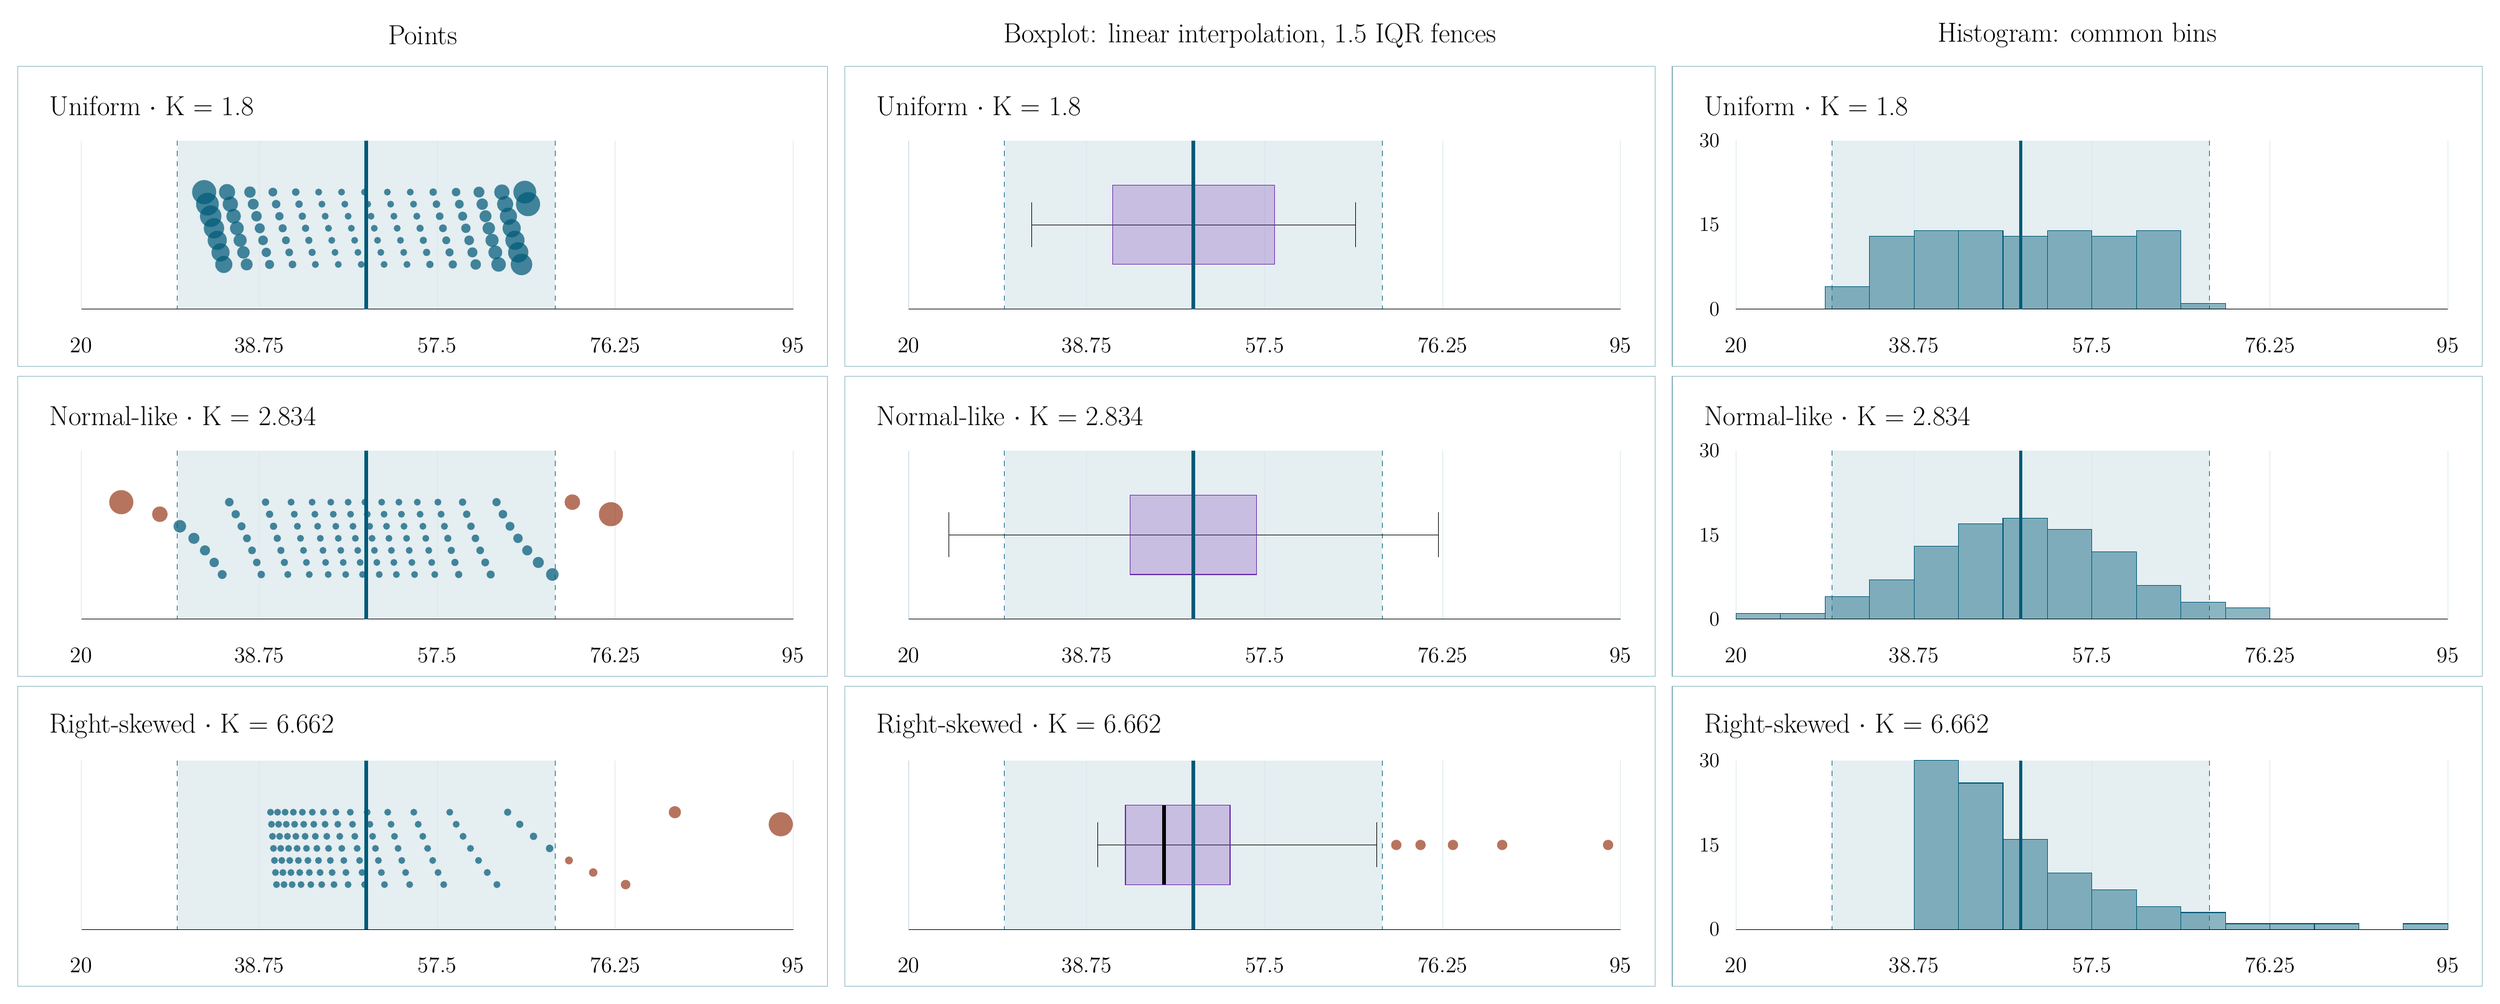
\begin{tikzpicture}[x=1pt,y=-1pt]
\node[anchor=center,font=\fontsize{16}{19}\selectfont] at (240,24) {Points};
\node[anchor=center,font=\fontsize{16}{19}\selectfont] at (720,24) {Boxplot: linear interpolation, 1.5 IQR fences};
\node[anchor=center,font=\fontsize{16}{19}\selectfont] at (1200,24) {Histogram: common bins};
\begin{scope}[shift={(0,40)}]
\path[draw=pcd1!45] (5,2) rectangle (475,176);
\node[anchor=west,font=\fontsize{16}{19}\selectfont] at (20,25) {Uniform \ensuremath{\cdot} K = 1.8};
\path[fill=pcd1,fill opacity=.1] (97.61871692665721,45) rectangle (316.78128307334276,143);
\draw[draw=pcd1,dashed] (97.61871692665721,45) -- (97.61871692665721,143);
\draw[draw=pcd1,dashed] (316.78128307334276,45) -- (316.78128307334276,143);
\draw[draw=pcd1!15] (42,45) -- (42,143);
\node[anchor=center,font=\fontsize{13}{16}\selectfont] at (42,164) {20};
\draw[draw=pcd1!15] (145.25,45) -- (145.25,143);
\node[anchor=center,font=\fontsize{13}{16}\selectfont] at (145.25,164) {38.75};
\draw[draw=pcd1!15] (248.5,45) -- (248.5,143);
\node[anchor=center,font=\fontsize{13}{16}\selectfont] at (248.5,164) {57.5};
\draw[draw=pcd1!15] (351.75,45) -- (351.75,143);
\node[anchor=center,font=\fontsize{13}{16}\selectfont] at (351.75,164) {76.25};
\draw[draw=pcd1!15] (455,45) -- (455,143);
\node[anchor=center,font=\fontsize{13}{16}\selectfont] at (455,164) {95};
\fill[pcd1,opacity=.72] (113.24412891739694,75) circle[radius=6.999999999999993pt];
\fill[pcd1,opacity=.72] (115.14222732310145,82) circle[radius=6.608039179759748pt];
\fill[pcd1,opacity=.72] (117.04032572881144,89) circle[radius=6.23958793041487pt];
\fill[pcd1,opacity=.72] (118.93842413452143,96) circle[radius=5.893686847606725pt];
\fill[pcd1,opacity=.72] (120.83652254023141,103) circle[radius=5.569396514566342pt];
\fill[pcd1,opacity=.72] (122.7346209459414,110) circle[radius=5.265797502115577pt];
\fill[pcd1,opacity=.72] (124.63271935165137,117) circle[radius=4.981990368667116pt];
\fill[pcd1,opacity=.72] (126.53081775736136,75) circle[radius=4.717095660224478pt];
\fill[pcd1,opacity=.72] (128.42891616306582,82) circle[radius=4.470253910382699pt];
\fill[pcd1,opacity=.72] (130.32701456877584,89) circle[radius=4.240625640325518pt];
\fill[pcd1,opacity=.72] (132.2251129744858,96) circle[radius=4.027391358829684pt];
\fill[pcd1,opacity=.72] (134.1232113801958,103) circle[radius=3.8297515622620297pt];
\fill[pcd1,opacity=.72] (136.02130978590577,110) circle[radius=3.6469267345802168pt];
\fill[pcd1,opacity=.72] (137.9194081916158,117) circle[radius=3.4781573473327363pt];
\fill[pcd1,opacity=.72] (139.81750659732575,75) circle[radius=3.322703859658908pt];
\fill[pcd1,opacity=.72] (141.71560500303025,82) circle[radius=3.179846718289276pt];
\fill[pcd1,opacity=.72] (143.61370340874024,89) circle[radius=3.048886357543997pt];
\fill[pcd1,opacity=.72] (145.51180181445022,96) circle[radius=2.929143199335308pt];
\fill[pcd1,opacity=.72] (147.4099002201602,103) circle[radius=2.8199576531658463pt];
\fill[pcd1,opacity=.72] (149.3079986258702,110) circle[radius=2.720690116129078pt];
\fill[pcd1,opacity=.72] (151.20609703158019,117) circle[radius=2.630720972909298pt];
\fill[pcd1,opacity=.72] (153.10419543729017,75) circle[radius=2.5494505957816322pt];
\fill[pcd1,opacity=.72] (155.00229384299465,82) circle[radius=2.476299344612234pt];
\fill[pcd1,opacity=.72] (156.90039224870463,89) circle[radius=2.410707566857463pt];
\fill[pcd1,opacity=.72] (158.79849065441462,96) circle[radius=2.352135597565156pt];
\fill[pcd1,opacity=.72] (160.6965890601246,103) circle[radius=2.300063759373754pt];
\fill[pcd1,opacity=.72] (162.59468746583457,110) circle[radius=2.2539923625125264pt];
\fill[pcd1,opacity=.72] (164.49278587154458,117) circle[radius=2.2134417048015735pt];
\fill[pcd1,opacity=.72] (166.39088427725454,75) circle[radius=2.177952071651825pt];
\fill[pcd1,opacity=.72] (168.28898268295902,82) circle[radius=2.1470837360651207pt];
\fill[pcd1,opacity=.72] (170.18708108866903,89) circle[radius=2.1204169586338706pt];
\fill[pcd1,opacity=.72] (172.085179494379,96) circle[radius=2.0975519875415864pt];
\fill[pcd1,opacity=.72] (173.98327790008898,103) circle[radius=2.078109058562514pt];
\fill[pcd1,opacity=.72] (175.88137630579897,110) circle[radius=2.0617283950617282pt];
\fill[pcd1,opacity=.72] (177.77947471150895,117) circle[radius=2.0480702079951327pt];
\fill[pcd1,opacity=.72] (179.67757311721897,75) circle[radius=2.0368146959094604pt];
\fill[pcd1,opacity=.72] (181.57567152292344,82) circle[radius=2.027662044942298pt];
\fill[pcd1,opacity=.72] (183.47376992863343,89) circle[radius=2.020332428821984pt];
\fill[pcd1,opacity=.72] (185.37186833434342,96) circle[radius=2.0145660088677686pt];
\fill[pcd1,opacity=.72] (187.2699667400534,103) circle[radius=2.0101229339897015pt];
\fill[pcd1,opacity=.72] (189.1680651457634,110) circle[radius=2.006783340688662pt];
\fill[pcd1,opacity=.72] (191.06616355147338,117) circle[radius=2.004347353056358pt];
\fill[pcd1,opacity=.72] (192.96426195718337,75) circle[radius=2.0026350827753268pt];
\fill[pcd1,opacity=.72] (194.8623603628878,82) circle[radius=2.0014866291189377pt];
\fill[pcd1,opacity=.72] (196.76045876859783,89) circle[radius=2.00076207895138pt];
\fill[pcd1,opacity=.72] (198.65855717430782,96) circle[radius=2.0003415067276826pt];
\fill[pcd1,opacity=.72] (200.55665558001778,103) circle[radius=2.0001249744937pt];
\fill[pcd1,opacity=.72] (202.4547539857278,110) circle[radius=2.000032531886115pt];
\fill[pcd1,opacity=.72] (204.35285239143775,117) circle[radius=2.0000042161324405pt];
\fill[pcd1,opacity=.72] (206.25095079714774,75) circle[radius=2.0000000520510177pt];
\fill[pcd1,opacity=.72] (208.14904920285224,82) circle[radius=2.0000000520510177pt];
\fill[pcd1,opacity=.72] (210.04714760856223,89) circle[radius=2.0000042161324405pt];
\fill[pcd1,opacity=.72] (211.94524601427224,96) circle[radius=2.000032531886115pt];
\fill[pcd1,opacity=.72] (213.8433444199822,103) circle[radius=2.0001249744937pt];
\fill[pcd1,opacity=.72] (215.74144282569222,110) circle[radius=2.0003415067276826pt];
\fill[pcd1,opacity=.72] (217.63954123140218,117) circle[radius=2.00076207895138pt];
\fill[pcd1,opacity=.72] (219.53763963711216,75) circle[radius=2.0014866291189377pt];
\fill[pcd1,opacity=.72] (221.43573804281664,82) circle[radius=2.0026350827753268pt];
\fill[pcd1,opacity=.72] (223.33383644852663,89) circle[radius=2.004347353056358pt];
\fill[pcd1,opacity=.72] (225.2319348542366,96) circle[radius=2.006783340688662pt];
\fill[pcd1,opacity=.72] (227.13003325994657,103) circle[radius=2.010122933989702pt];
\fill[pcd1,opacity=.72] (229.0281316656566,110) circle[radius=2.014566008867769pt];
\fill[pcd1,opacity=.72] (230.92623007136655,117) circle[radius=2.0203324288219844pt];
\fill[pcd1,opacity=.72] (232.82432847707656,75) circle[radius=2.0276620449422986pt];
\fill[pcd1,opacity=.72] (234.722426882781,82) circle[radius=2.036814695909461pt];
\fill[pcd1,opacity=.72] (236.62052528849105,89) circle[radius=2.048070207995133pt];
\fill[pcd1,opacity=.72] (238.51862369420104,96) circle[radius=2.0617283950617287pt];
\fill[pcd1,opacity=.72] (240.416722099911,103) circle[radius=2.078109058562515pt];
\fill[pcd1,opacity=.72] (242.31482050562101,110) circle[radius=2.0975519875415873pt];
\fill[pcd1,opacity=.72] (244.21291891133097,117) circle[radius=2.1204169586338715pt];
\fill[pcd1,opacity=.72] (246.11101731704096,75) circle[radius=2.147083736065122pt];
\fill[pcd1,opacity=.72] (248.00911572274543,82) circle[radius=2.177952071651826pt];
\fill[pcd1,opacity=.72] (249.90721412845545,89) circle[radius=2.2134417048015753pt];
\fill[pcd1,opacity=.72] (251.8053125341654,96) circle[radius=2.253992362512528pt];
\fill[pcd1,opacity=.72] (253.7034109398754,103) circle[radius=2.3000637593737556pt];
\fill[pcd1,opacity=.72] (255.6015093455854,110) circle[radius=2.3521355975651583pt];
\fill[pcd1,opacity=.72] (257.49960775129534,117) circle[radius=2.410707566857466pt];
\fill[pcd1,opacity=.72] (259.39770615700536,75) circle[radius=2.476299344612237pt];
\fill[pcd1,opacity=.72] (261.2958045627098,82) circle[radius=2.5494505957816354pt];
\fill[pcd1,opacity=.72] (263.1939029684198,89) circle[radius=2.6307209729093017pt];
\fill[pcd1,opacity=.72] (265.09200137412984,96) circle[radius=2.7206901161290817pt];
\fill[pcd1,opacity=.72] (266.9900997798398,103) circle[radius=2.8199576531658503pt];
\fill[pcd1,opacity=.72] (268.88819818554975,110) circle[radius=2.9291431993353125pt];
\fill[pcd1,opacity=.72] (270.78629659125977,117) circle[radius=3.048886357544002pt];
\fill[pcd1,opacity=.72] (272.6843949969698,75) circle[radius=3.179846718289282pt];
\fill[pcd1,opacity=.72] (274.58249340267423,82) circle[radius=3.3227038596589136pt];
\fill[pcd1,opacity=.72] (276.48059180838425,89) circle[radius=3.4781573473327425pt];
\fill[pcd1,opacity=.72] (278.3786902140942,96) circle[radius=3.6469267345802243pt];
\fill[pcd1,opacity=.72] (280.27678861980417,103) circle[radius=3.8297515622620377pt];
\fill[pcd1,opacity=.72] (282.1748870255142,110) circle[radius=4.027391358829693pt];
\fill[pcd1,opacity=.72] (284.0729854312242,117) circle[radius=4.2406256403255265pt];
\fill[pcd1,opacity=.72] (285.97108383693416,75) circle[radius=4.4702539103827075pt];
\fill[pcd1,opacity=.72] (287.86918224263866,82) circle[radius=4.717095660224494pt];
\fill[pcd1,opacity=.72] (289.7672806483487,89) circle[radius=4.981990368667134pt];
\fill[pcd1,opacity=.72] (291.6653790540587,96) circle[radius=5.2657975021155945pt];
\fill[pcd1,opacity=.72] (293.5634774597686,103) circle[radius=5.569396514566361pt];
\fill[pcd1,opacity=.72] (295.4615758654786,110) circle[radius=5.893686847606746pt];
\fill[pcd1,opacity=.72] (297.3596742711886,117) circle[radius=6.239587930414892pt];
\fill[pcd1,opacity=.72] (299.25777267689307,75) circle[radius=6.608039179758658pt];
\fill[pcd1,opacity=.72] (301.155871082603,82) circle[radius=7pt];
\draw[draw=black] (42,143) -- (455,143);
\draw[draw=pcd1,line width=2pt] (207.19999999999996,45) -- (207.19999999999996,143);
\end{scope}
\begin{scope}[shift={(480,40)}]
\path[draw=pcd1!45] (5,2) rectangle (475,176);
\node[anchor=west,font=\fontsize{16}{19}\selectfont] at (20,25) {Uniform \ensuremath{\cdot} K = 1.8};
\path[fill=pcd1,fill opacity=.1] (97.61871692665721,45) rectangle (316.78128307334276,143);
\draw[draw=pcd1,dashed] (97.61871692665721,45) -- (97.61871692665721,143);
\draw[draw=pcd1,dashed] (316.78128307334276,45) -- (316.78128307334276,143);
\draw[draw=pcd1!15] (42,45) -- (42,143);
\node[anchor=center,font=\fontsize{13}{16}\selectfont] at (42,164) {20};
\draw[draw=pcd1!15] (145.25,45) -- (145.25,143);
\node[anchor=center,font=\fontsize{13}{16}\selectfont] at (145.25,164) {38.75};
\draw[draw=pcd1!15] (248.5,45) -- (248.5,143);
\node[anchor=center,font=\fontsize{13}{16}\selectfont] at (248.5,164) {57.5};
\draw[draw=pcd1!15] (351.75,45) -- (351.75,143);
\node[anchor=center,font=\fontsize{13}{16}\selectfont] at (351.75,164) {76.25};
\draw[draw=pcd1!15] (455,45) -- (455,143);
\node[anchor=center,font=\fontsize{13}{16}\selectfont] at (455,164) {95};
\draw[draw=black] (113.24412891739694,94) -- (301.155871082603,94);
\path[fill=pcd2,fill opacity=.25,draw=pcd2] (160.22206445869708,71) rectangle (254.1779355413029,117);
\draw[draw=black,line width=2pt] (207.20000000000002,71) -- (207.20000000000002,117);
\draw[draw=black] (113.24412891739694,81) -- (113.24412891739694,107);
\draw[draw=black] (301.155871082603,81) -- (301.155871082603,107);
\draw[draw=black] (42,143) -- (455,143);
\draw[draw=pcd1,line width=2pt] (207.19999999999996,45) -- (207.19999999999996,143);
\end{scope}
\begin{scope}[shift={(960,40)}]
\path[draw=pcd1!45] (5,2) rectangle (475,176);
\node[anchor=west,font=\fontsize{16}{19}\selectfont] at (20,25) {Uniform \ensuremath{\cdot} K = 1.8};
\path[fill=pcd1,fill opacity=.1] (97.61871692665721,45) rectangle (316.78128307334276,143);
\draw[draw=pcd1,dashed] (97.61871692665721,45) -- (97.61871692665721,143);
\draw[draw=pcd1,dashed] (316.78128307334276,45) -- (316.78128307334276,143);
\draw[draw=pcd1!15] (42,45) -- (42,143);
\node[anchor=center,font=\fontsize{13}{16}\selectfont] at (42,164) {20};
\draw[draw=pcd1!15] (145.25,45) -- (145.25,143);
\node[anchor=center,font=\fontsize{13}{16}\selectfont] at (145.25,164) {38.75};
\draw[draw=pcd1!15] (248.5,45) -- (248.5,143);
\node[anchor=center,font=\fontsize{13}{16}\selectfont] at (248.5,164) {57.5};
\draw[draw=pcd1!15] (351.75,45) -- (351.75,143);
\node[anchor=center,font=\fontsize{13}{16}\selectfont] at (351.75,164) {76.25};
\draw[draw=pcd1!15] (455,45) -- (455,143);
\node[anchor=center,font=\fontsize{13}{16}\selectfont] at (455,164) {95};
\path[fill=pcd1,fill opacity=.45,draw=pcd1] (42,143) rectangle (67.8125,143);
\path[fill=pcd1,fill opacity=.45,draw=pcd1] (67.8125,143) rectangle (93.625,143);
\path[fill=pcd1,fill opacity=.45,draw=pcd1] (93.625,129.93333333333334) rectangle (119.4375,143);
\path[fill=pcd1,fill opacity=.45,draw=pcd1] (119.4375,100.53333333333333) rectangle (145.25,143);
\path[fill=pcd1,fill opacity=.45,draw=pcd1] (145.25,97.26666666666667) rectangle (171.0625,143);
\path[fill=pcd1,fill opacity=.45,draw=pcd1] (171.0625,97.26666666666667) rectangle (196.875,143);
\path[fill=pcd1,fill opacity=.45,draw=pcd1] (196.875,100.53333333333333) rectangle (222.6875,143);
\path[fill=pcd1,fill opacity=.45,draw=pcd1] (222.6875,97.26666666666667) rectangle (248.5,143);
\path[fill=pcd1,fill opacity=.45,draw=pcd1] (248.5,100.53333333333333) rectangle (274.3125,143);
\path[fill=pcd1,fill opacity=.45,draw=pcd1] (274.3125,97.26666666666667) rectangle (300.125,143);
\path[fill=pcd1,fill opacity=.45,draw=pcd1] (300.125,139.73333333333332) rectangle (325.9375,143);
\path[fill=pcd1,fill opacity=.45,draw=pcd1] (325.9375,143) rectangle (351.75,143);
\path[fill=pcd1,fill opacity=.45,draw=pcd1] (351.75,143) rectangle (377.5625,143);
\path[fill=pcd1,fill opacity=.45,draw=pcd1] (377.5625,143) rectangle (403.375,143);
\path[fill=pcd1,fill opacity=.45,draw=pcd1] (403.375,143) rectangle (429.1875,143);
\path[fill=pcd1,fill opacity=.45,draw=pcd1] (429.1875,143) rectangle (455,143);
\node[anchor=east,font=\fontsize{12}{15}\selectfont] at (36,143) {0};
\node[anchor=east,font=\fontsize{12}{15}\selectfont] at (36,94) {15};
\node[anchor=east,font=\fontsize{12}{15}\selectfont] at (36,45) {30};
\draw[draw=black] (42,143) -- (455,143);
\draw[draw=pcd1,line width=2pt] (207.19999999999996,45) -- (207.19999999999996,143);
\end{scope}
\begin{scope}[shift={(0,220)}]
\path[draw=pcd1!45] (5,2) rectangle (475,176);
\node[anchor=west,font=\fontsize{16}{19}\selectfont] at (20,25) {Normal-like \ensuremath{\cdot} K = 2.834};
\path[fill=pcd1,fill opacity=.1] (97.61871692665724,45) rectangle (316.78128307334276,143);
\draw[draw=pcd1,dashed] (97.61871692665724,45) -- (97.61871692665724,143);
\draw[draw=pcd1,dashed] (316.78128307334276,45) -- (316.78128307334276,143);
\draw[draw=pcd1!15] (42,45) -- (42,143);
\node[anchor=center,font=\fontsize{13}{16}\selectfont] at (42,164) {20};
\draw[draw=pcd1!15] (145.25,45) -- (145.25,143);
\node[anchor=center,font=\fontsize{13}{16}\selectfont] at (145.25,164) {38.75};
\draw[draw=pcd1!15] (248.5,45) -- (248.5,143);
\node[anchor=center,font=\fontsize{13}{16}\selectfont] at (248.5,164) {57.5};
\draw[draw=pcd1!15] (351.75,45) -- (351.75,143);
\node[anchor=center,font=\fontsize{13}{16}\selectfont] at (351.75,164) {76.25};
\draw[draw=pcd1!15] (455,45) -- (455,143);
\node[anchor=center,font=\fontsize{13}{16}\selectfont] at (455,164) {95};
\fill[pcd4,opacity=.72] (65.16454133626237,75) circle[radius=7pt];
\fill[pcd4,opacity=.72] (87.53765215058463,82) circle[radius=4.518911858822151pt];
\fill[pcd1,opacity=.72] (99.12436660107437,89) circle[radius=3.6760773226105625pt];
\fill[pcd1,opacity=.72] (107.28826938338861,96) circle[radius=3.2241899751733842pt];
\fill[pcd1,opacity=.72] (113.7129855211349,103) circle[radius=2.938400121095196pt];
\fill[pcd1,opacity=.72] (119.0730051912103,110) circle[radius=2.7410008987020733pt];
\fill[pcd1,opacity=.72] (123.70993496528129,117) circle[radius=2.5969281907949724pt];
\fill[pcd1,opacity=.72] (127.82187022489454,75) circle[radius=2.4877377172879798pt];
\fill[pcd1,opacity=.72] (131.53442809166978,82) circle[radius=2.4026949358340897pt];
\fill[pcd1,opacity=.72] (134.93251509506104,89) circle[radius=2.335084742786061pt];
\fill[pcd1,opacity=.72] (138.07634270918393,96) circle[radius=2.28047213828002pt];
\fill[pcd1,opacity=.72] (141.01024094780104,103) circle[radius=2.2358012444414985pt];
\fill[pcd1,opacity=.72] (143.76784568754908,110) circle[radius=2.198893567479063pt];
\fill[pcd1,opacity=.72] (146.37531884246346,117) circle[radius=2.168152084851331pt];
\fill[pcd1,opacity=.72] (148.85343600881788,75) circle[radius=2.142378375978222pt];
\fill[pcd1,opacity=.72] (151.21898956004614,82) circle[radius=2.1206551390509336pt];
\fill[pcd1,opacity=.72] (153.48576081178732,89) circle[radius=2.1022681988276832pt];
\fill[pcd1,opacity=.72] (155.66521140319736,96) circle[radius=2.0866532563115694pt];
\fill[pcd1,opacity=.72] (157.7669862283159,103) circle[radius=2.073358635955626pt];
\fill[pcd1,opacity=.72] (159.7992865920125,110) circle[radius=2.062018663730591pt];
\fill[pcd1,opacity=.72] (161.76915195659856,117) circle[radius=2.0523342816192836pt];
\fill[pcd1,opacity=.72] (163.68267600478754,75) circle[radius=2.044058693862128pt];
\fill[pcd1,opacity=.72] (165.54517465782482,82) circle[radius=2.036986578956139pt];
\fill[pcd1,opacity=.72] (167.36131838621117,89) circle[radius=2.030945871902878pt];
\fill[pcd1,opacity=.72] (169.1352375982878,96) circle[radius=2.02579142781324pt];
\fill[pcd1,opacity=.72] (170.87060746462737,103) circle[radius=2.0214000819508358pt];
\fill[pcd1,opacity=.72] (172.5707168478382,110) circle[radius=2.0176667595446003pt];
\fill[pcd1,opacity=.72] (174.2385248135968,117) circle[radius=2.0145013840085375pt];
\fill[pcd1,opacity=.72] (175.87670734235186,75) circle[radius=2.0118263989368326pt];
\fill[pcd1,opacity=.72] (177.4876962383739,82) circle[radius=2.009574766635206pt];
\fill[pcd1,opacity=.72] (179.07371177394688,89) circle[radius=2.007688340053202pt];
\fill[pcd1,opacity=.72] (180.63679026512506,96) circle[radius=2.0061165298218606pt];
\fill[pcd1,opacity=.72] (182.17880751793538,103) circle[radius=2.0048152063997735pt];
\fill[pcd1,opacity=.72] (183.7014988885424,110) circle[radius=2.003745790951232pt];
\fill[pcd1,opacity=.72] (185.20647655075038,117) circle[radius=2.0028744988197538pt];
\fill[pcd1,opacity=.72] (186.69524444809016,75) circle[radius=2.002171707228842pt];
\fill[pcd1,opacity=.72] (188.16921131713553,82) circle[radius=2.0016114247872006pt];
\fill[pcd1,opacity=.72] (189.62970209763023,89) circle[radius=2.0011708449633pt];
\fill[pcd1,opacity=.72] (191.07796798874614,96) circle[radius=2.000829969262336pt];
\fill[pcd1,opacity=.72] (192.51519536587472,103) circle[radius=2.000571288634967pt];
\fill[pcd1,opacity=.72] (193.94251373685682,110) circle[radius=2.0003795138549374pt];
\fill[pcd1,opacity=.72] (195.36100288752172,117) circle[radius=2.000241347358945pt];
\fill[pcd1,opacity=.72] (196.77169934342442,75) circle[radius=2.000145290449422pt];
\fill[pcd1,opacity=.72] (198.17560225582272,82) circle[radius=2.000081480897744pt];
\fill[pcd1,opacity=.72] (199.57367880477972,89) circle[radius=2.000041556911326pt];
\fill[pcd1,opacity=.72] (200.96686920014255,96) circle[radius=2.0000185441893934pt];
\fill[pcd1,opacity=.72] (202.3560913510083,103) circle[radius=2.0000067634248526pt];
\fill[pcd1,opacity=.72] (203.74224526671262,110) circle[radius=2.000001756142002pt];
\fill[pcd1,opacity=.72] (205.1262172457786,117) circle[radius=2.000000227214439pt];
\fill[pcd1,opacity=.72] (206.50888390477604,75) circle[radius=2.0000000028027665pt];
\fill[pcd1,opacity=.72] (207.89111609522396,82) circle[radius=2.0000000028027665pt];
\fill[pcd1,opacity=.72] (209.27378275422137,89) circle[radius=2.000000227214439pt];
\fill[pcd1,opacity=.72] (210.6577547332874,96) circle[radius=2.000001756142002pt];
\fill[pcd1,opacity=.72] (212.0439086489917,103) circle[radius=2.0000067634248526pt];
\fill[pcd1,opacity=.72] (213.43313079985745,110) circle[radius=2.0000185441893934pt];
\fill[pcd1,opacity=.72] (214.8263211952203,117) circle[radius=2.000041556911326pt];
\fill[pcd1,opacity=.72] (216.22439774417728,75) circle[radius=2.000081480897744pt];
\fill[pcd1,opacity=.72] (217.62830065657556,82) circle[radius=2.000145290449422pt];
\fill[pcd1,opacity=.72] (219.03899711247826,89) circle[radius=2.000241347358945pt];
\fill[pcd1,opacity=.72] (220.45748626314318,96) circle[radius=2.0003795138549374pt];
\fill[pcd1,opacity=.72] (221.8848046341253,103) circle[radius=2.000571288634967pt];
\fill[pcd1,opacity=.72] (223.32203201125384,110) circle[radius=2.000829969262336pt];
\fill[pcd1,opacity=.72] (224.77029790236978,117) circle[radius=2.0011708449633pt];
\fill[pcd1,opacity=.72] (226.23078868286447,75) circle[radius=2.0016114247872006pt];
\fill[pcd1,opacity=.72] (227.70475555190984,82) circle[radius=2.002171707228842pt];
\fill[pcd1,opacity=.72] (229.1935234492496,89) circle[radius=2.0028744988197538pt];
\fill[pcd1,opacity=.72] (230.6985011114576,96) circle[radius=2.003745790951232pt];
\fill[pcd1,opacity=.72] (232.22119248206462,103) circle[radius=2.0048152063997735pt];
\fill[pcd1,opacity=.72] (233.76320973487495,110) circle[radius=2.0061165298218606pt];
\fill[pcd1,opacity=.72] (235.3262882260531,117) circle[radius=2.007688340053202pt];
\fill[pcd1,opacity=.72] (236.91230376162608,75) circle[radius=2.009574766635206pt];
\fill[pcd1,opacity=.72] (238.52329265764814,82) circle[radius=2.0118263989368326pt];
\fill[pcd1,opacity=.72] (240.16147518640324,89) circle[radius=2.0145013840085375pt];
\fill[pcd1,opacity=.72] (241.8292831521618,96) circle[radius=2.0176667595446003pt];
\fill[pcd1,opacity=.72] (243.52939253537264,103) circle[radius=2.0214000819508358pt];
\fill[pcd1,opacity=.72] (245.2647624017122,110) circle[radius=2.02579142781324pt];
\fill[pcd1,opacity=.72] (247.03868161378887,117) circle[radius=2.030945871902878pt];
\fill[pcd1,opacity=.72] (248.8548253421752,75) circle[radius=2.036986578956139pt];
\fill[pcd1,opacity=.72] (250.71732399521247,82) circle[radius=2.044058693862128pt];
\fill[pcd1,opacity=.72] (252.63084804340141,89) circle[radius=2.0523342816192836pt];
\fill[pcd1,opacity=.72] (254.60071340798754,96) circle[radius=2.062018663730591pt];
\fill[pcd1,opacity=.72] (256.6330137716841,103) circle[radius=2.073358635955626pt];
\fill[pcd1,opacity=.72] (258.7347885968027,110) circle[radius=2.0866532563115694pt];
\fill[pcd1,opacity=.72] (260.9142391882127,117) circle[radius=2.1022681988276832pt];
\fill[pcd1,opacity=.72] (263.18101043995387,75) circle[radius=2.1206551390509336pt];
\fill[pcd1,opacity=.72] (265.5465639911821,82) circle[radius=2.142378375978222pt];
\fill[pcd1,opacity=.72] (268.0246811575365,89) circle[radius=2.168152084851331pt];
\fill[pcd1,opacity=.72] (270.63215431245095,96) circle[radius=2.198893567479063pt];
\fill[pcd1,opacity=.72] (273.389759052199,103) circle[radius=2.2358012444414985pt];
\fill[pcd1,opacity=.72] (276.3236572908161,110) circle[radius=2.28047213828002pt];
\fill[pcd1,opacity=.72] (279.46748490493894,117) circle[radius=2.335084742786061pt];
\fill[pcd1,opacity=.72] (282.86557190833025,75) circle[radius=2.4026949358340897pt];
\fill[pcd1,opacity=.72] (286.5781297751055,82) circle[radius=2.4877377172879807pt];
\fill[pcd1,opacity=.72] (290.6900650347187,89) circle[radius=2.5969281907949724pt];
\fill[pcd1,opacity=.72] (295.3269948087898,96) circle[radius=2.7410008987020746pt];
\fill[pcd1,opacity=.72] (300.6870144788651,103) circle[radius=2.938400121095195pt];
\fill[pcd1,opacity=.72] (307.1117306166114,110) circle[radius=3.2241899751733842pt];
\fill[pcd1,opacity=.72] (315.27563339892566,117) circle[radius=3.676077322610565pt];
\fill[pcd4,opacity=.72] (326.86234784941536,75) circle[radius=4.518911858822153pt];
\fill[pcd4,opacity=.72] (349.2354586637376,82) circle[radius=6.999999999999995pt];
\draw[draw=black] (42,143) -- (455,143);
\draw[draw=pcd1,line width=2pt] (207.20000000000002,45) -- (207.20000000000002,143);
\end{scope}
\begin{scope}[shift={(480,220)}]
\path[draw=pcd1!45] (5,2) rectangle (475,176);
\node[anchor=west,font=\fontsize{16}{19}\selectfont] at (20,25) {Normal-like \ensuremath{\cdot} K = 2.834};
\path[fill=pcd1,fill opacity=.1] (97.61871692665724,45) rectangle (316.78128307334276,143);
\draw[draw=pcd1,dashed] (97.61871692665724,45) -- (97.61871692665724,143);
\draw[draw=pcd1,dashed] (316.78128307334276,45) -- (316.78128307334276,143);
\draw[draw=pcd1!15] (42,45) -- (42,143);
\node[anchor=center,font=\fontsize{13}{16}\selectfont] at (42,164) {20};
\draw[draw=pcd1!15] (145.25,45) -- (145.25,143);
\node[anchor=center,font=\fontsize{13}{16}\selectfont] at (145.25,164) {38.75};
\draw[draw=pcd1!15] (248.5,45) -- (248.5,143);
\node[anchor=center,font=\fontsize{13}{16}\selectfont] at (248.5,164) {57.5};
\draw[draw=pcd1!15] (351.75,45) -- (351.75,143);
\node[anchor=center,font=\fontsize{13}{16}\selectfont] at (351.75,164) {76.25};
\draw[draw=pcd1!15] (455,45) -- (455,143);
\node[anchor=center,font=\fontsize{13}{16}\selectfont] at (455,164) {95};
\draw[draw=black] (65.16454133626237,94) -- (349.2354586637376,94);
\path[fill=pcd2,fill opacity=.25,draw=pcd2] (170.43676499804246,71) rectangle (243.96323500195754,117);
\draw[draw=black,line width=2pt] (207.20000000000002,71) -- (207.20000000000002,117);
\draw[draw=black] (65.16454133626237,81) -- (65.16454133626237,107);
\draw[draw=black] (349.2354586637376,81) -- (349.2354586637376,107);
\draw[draw=black] (42,143) -- (455,143);
\draw[draw=pcd1,line width=2pt] (207.20000000000002,45) -- (207.20000000000002,143);
\end{scope}
\begin{scope}[shift={(960,220)}]
\path[draw=pcd1!45] (5,2) rectangle (475,176);
\node[anchor=west,font=\fontsize{16}{19}\selectfont] at (20,25) {Normal-like \ensuremath{\cdot} K = 2.834};
\path[fill=pcd1,fill opacity=.1] (97.61871692665724,45) rectangle (316.78128307334276,143);
\draw[draw=pcd1,dashed] (97.61871692665724,45) -- (97.61871692665724,143);
\draw[draw=pcd1,dashed] (316.78128307334276,45) -- (316.78128307334276,143);
\draw[draw=pcd1!15] (42,45) -- (42,143);
\node[anchor=center,font=\fontsize{13}{16}\selectfont] at (42,164) {20};
\draw[draw=pcd1!15] (145.25,45) -- (145.25,143);
\node[anchor=center,font=\fontsize{13}{16}\selectfont] at (145.25,164) {38.75};
\draw[draw=pcd1!15] (248.5,45) -- (248.5,143);
\node[anchor=center,font=\fontsize{13}{16}\selectfont] at (248.5,164) {57.5};
\draw[draw=pcd1!15] (351.75,45) -- (351.75,143);
\node[anchor=center,font=\fontsize{13}{16}\selectfont] at (351.75,164) {76.25};
\draw[draw=pcd1!15] (455,45) -- (455,143);
\node[anchor=center,font=\fontsize{13}{16}\selectfont] at (455,164) {95};
\path[fill=pcd1,fill opacity=.45,draw=pcd1] (42,139.73333333333332) rectangle (67.8125,143);
\path[fill=pcd1,fill opacity=.45,draw=pcd1] (67.8125,139.73333333333332) rectangle (93.625,143);
\path[fill=pcd1,fill opacity=.45,draw=pcd1] (93.625,129.93333333333334) rectangle (119.4375,143);
\path[fill=pcd1,fill opacity=.45,draw=pcd1] (119.4375,120.13333333333333) rectangle (145.25,143);
\path[fill=pcd1,fill opacity=.45,draw=pcd1] (145.25,100.53333333333333) rectangle (171.0625,143);
\path[fill=pcd1,fill opacity=.45,draw=pcd1] (171.0625,87.46666666666667) rectangle (196.875,143);
\path[fill=pcd1,fill opacity=.45,draw=pcd1] (196.875,84.2) rectangle (222.6875,143);
\path[fill=pcd1,fill opacity=.45,draw=pcd1] (222.6875,90.73333333333333) rectangle (248.5,143);
\path[fill=pcd1,fill opacity=.45,draw=pcd1] (248.5,103.8) rectangle (274.3125,143);
\path[fill=pcd1,fill opacity=.45,draw=pcd1] (274.3125,123.4) rectangle (300.125,143);
\path[fill=pcd1,fill opacity=.45,draw=pcd1] (300.125,133.2) rectangle (325.9375,143);
\path[fill=pcd1,fill opacity=.45,draw=pcd1] (325.9375,136.46666666666667) rectangle (351.75,143);
\path[fill=pcd1,fill opacity=.45,draw=pcd1] (351.75,143) rectangle (377.5625,143);
\path[fill=pcd1,fill opacity=.45,draw=pcd1] (377.5625,143) rectangle (403.375,143);
\path[fill=pcd1,fill opacity=.45,draw=pcd1] (403.375,143) rectangle (429.1875,143);
\path[fill=pcd1,fill opacity=.45,draw=pcd1] (429.1875,143) rectangle (455,143);
\node[anchor=east,font=\fontsize{12}{15}\selectfont] at (36,143) {0};
\node[anchor=east,font=\fontsize{12}{15}\selectfont] at (36,94) {15};
\node[anchor=east,font=\fontsize{12}{15}\selectfont] at (36,45) {30};
\draw[draw=black] (42,143) -- (455,143);
\draw[draw=pcd1,line width=2pt] (207.20000000000002,45) -- (207.20000000000002,143);
\end{scope}
\begin{scope}[shift={(0,400)}]
\path[draw=pcd1!45] (5,2) rectangle (475,176);
\node[anchor=west,font=\fontsize{16}{19}\selectfont] at (20,25) {Right-skewed \ensuremath{\cdot} K = 6.662};
\path[fill=pcd1,fill opacity=.1] (97.61871692665778,45) rectangle (316.78128307334214,143);
\draw[draw=pcd1,dashed] (97.61871692665778,45) -- (97.61871692665778,143);
\draw[draw=pcd1,dashed] (316.78128307334214,45) -- (316.78128307334214,143);
\draw[draw=pcd1!15] (42,45) -- (42,143);
\node[anchor=center,font=\fontsize{13}{16}\selectfont] at (42,164) {20};
\draw[draw=pcd1!15] (145.25,45) -- (145.25,143);
\node[anchor=center,font=\fontsize{13}{16}\selectfont] at (145.25,164) {38.75};
\draw[draw=pcd1!15] (248.5,45) -- (248.5,143);
\node[anchor=center,font=\fontsize{13}{16}\selectfont] at (248.5,164) {57.5};
\draw[draw=pcd1!15] (351.75,45) -- (351.75,143);
\node[anchor=center,font=\fontsize{13}{16}\selectfont] at (351.75,164) {76.25};
\draw[draw=pcd1!15] (455,45) -- (455,143);
\node[anchor=center,font=\fontsize{13}{16}\selectfont] at (455,164) {95};
\fill[pcd1,opacity=.72] (151.74905333266133,75) circle[radius=2.0141121726971813pt];
\fill[pcd1,opacity=.72] (152.31395571301317,82) circle[radius=2.013545834018063pt];
\fill[pcd1,opacity=.72] (152.8846225028966,89) circle[radius=2.0129911988990723pt];
\fill[pcd1,opacity=.72] (153.4611725592456,96) circle[radius=2.0124483206683546pt];
\fill[pcd1,opacity=.72] (154.04372845340623,103) circle[radius=2.011917250498611pt];
\fill[pcd1,opacity=.72] (154.63241662752557,110) circle[radius=2.0113980372402436pt];
\fill[pcd1,opacity=.72] (155.22736755930603,117) circle[radius=2.010890727244706pt];
\fill[pcd1,opacity=.72] (155.8287159355586,75) circle[radius=2.0103953641776195pt];
\fill[pcd1,opacity=.72] (156.4366008352228,82) circle[radius=2.009911988820997pt];
\fill[pcd1,opacity=.72] (157.0511659224521,89) circle[radius=2.0094406388640036pt];
\fill[pcd1,opacity=.72] (157.67255965038294,96) circle[radius=2.008981348681674pt];
\fill[pcd1,opacity=.72] (158.3009354764065,103) circle[radius=2.0085341491008486pt];
\fill[pcd1,opacity=.72] (158.93645208964392,110) circle[radius=2.008099067152723pt];
\fill[pcd1,opacity=.72] (159.5792736514773,117) circle[radius=2.0076761258112836pt];
\fill[pcd1,opacity=.72] (160.22957005010642,75) circle[radius=2.0072653437168593pt];
\fill[pcd1,opacity=.72] (160.88751717007247,82) circle[radius=2.006866734884059pt];
\fill[pcd1,opacity=.72] (161.55329717777346,89) circle[radius=2.006480308393336pt];
\fill[pcd1,opacity=.72] (162.22709882426457,96) circle[radius=2.0061060680652925pt];
\fill[pcd1,opacity=.72] (162.90911776645657,103) circle[radius=2.0057440121169843pt];
\fill[pcd1,opacity=.72] (163.59955690818776,110) circle[radius=2.00539413279933pt];
\fill[pcd1,opacity=.72] (164.2986267625626,117) circle[radius=2.0050564160148276pt];
\fill[pcd1,opacity=.72] (165.00654583728073,75) circle[radius=2.0047308409146756pt];
\fill[pcd1,opacity=.72] (165.7235410446304,82) circle[radius=2.0044173794745173pt];
\fill[pcd1,opacity=.72] (166.44984813813954,89) circle[radius=2.004115996047957pt];
\fill[pcd1,opacity=.72] (167.1857121779055,96) circle[radius=2.0038266468971067pt];
\fill[pcd1,opacity=.72] (167.93138802701577,103) circle[radius=2.003549279699394pt];
\fill[pcd1,opacity=.72] (168.68714088144333,110) circle[radius=2.0032838330300398pt];
\fill[pcd1,opacity=.72] (169.4532468363193,117) circle[radius=2.0030302358196126pt];
\fill[pcd1,opacity=.72] (170.229993491435,75) circle[radius=2.0027884067863146pt];
\fill[pcd1,opacity=.72] (171.01768059949208,82) circle[radius=2.0025582538427176pt];
\fill[pcd1,opacity=.72] (171.8166207605925,89) circle[radius=2.002339673477005pt];
\fill[pcd1,opacity=.72] (172.6271401670594,96) circle[radius=2.0021325501090064pt];
\fill[pcd1,opacity=.72] (173.44957940309263,103) circle[radius=2.0019367554216605pt];
\fill[pcd1,opacity=.72] (174.28429430402963,110) circle[radius=2.0017521476690714pt];
\fill[pcd1,opacity=.72] (175.13165688074383,117) circle[radius=2.001578570962806pt];
\fill[pcd1,opacity=.72] (175.99205631517825,75) circle[radius=2.001415854538812pt];
\fill[pcd1,opacity=.72] (176.86590003362252,82) circle[radius=2.0012638120082142pt];
\fill[pcd1,opacity=.72] (177.753614865211,89) circle[radius=2.0011222405962403pt];
\fill[pcd1,opacity=.72] (178.65564829385775,96) circle[radius=2.000990920374876pt];
\fill[pcd1,opacity=.72] (179.57246981280298,103) circle[radius=2.0008696134963815pt];
\fill[pcd1,opacity=.72] (180.5045723920573,110) circle[radius=2.000758063436755pt];
\fill[pcd1,opacity=.72] (181.45247407026855,117) circle[radius=2.0006559942605615pt];
\fill[pcd1,opacity=.72] (182.41671968376033,75) circle[radius=2.000563109921442pt];
\fill[pcd1,opacity=.72] (183.39788274731754,82) circle[radius=2.000479093616113pt];
\fill[pcd1,opacity=.72] (184.3965675029305,89) circle[radius=2.0004036072139657pt];
\fill[pcd1,opacity=.72] (185.41341115475836,96) circle[radius=2.0003362907896243pt];
\fill[pcd1,opacity=.72] (186.44908631115385,103) circle[radius=2.000276762292238pt];
\fill[pcd1,opacity=.72] (187.5043036570159,110) circle[radius=2.000224617393159pt];
\fill[pcd1,opacity=.72] (188.5798148832203,117) circle[radius=2.0001794295632958pt];
\fill[pcd1,opacity=.72] (189.6764159032678,75) circle[radius=2.0001407504433115pt];
\fill[pcd1,opacity=.72] (190.79495039163652,82) circle[radius=2.000108110584404pt];
\fill[pcd1,opacity=.72] (191.93631368331717,89) circle[radius=2.0000810206554105pt];
\fill[pcd1,opacity=.72] (193.10145707959668,96) circle[radius=2.0000589732342178pt];
\fill[pcd1,opacity=.72] (194.29139261200237,103) circle[radius=2.000041445328963pt];
\fill[pcd1,opacity=.72] (195.50719832418628,110) circle[radius=2.000027901808729pt];
\fill[pcd1,opacity=.72] (196.75002414084807,117) circle[radius=2.0000177999659523pt];
\fill[pcd1,opacity=.72] (198.02109840369124,75) circle[radius=2.000010595485922pt];
\fill[pcd1,opacity=.72] (199.32173516762984,82) circle[radius=2.0000057501652533pt];
\fill[pcd1,opacity=.72] (200.65334236577635,89) circle[radius=2.0000027418048547pt];
\fill[pcd1,opacity=.72] (202.01743097046457,96) circle[radius=2.000001076808325pt];
\fill[pcd1,opacity=.72] (203.41562529973626,103) circle[radius=2.000000306150198pt];
\fill[pcd1,opacity=.72] (204.8496746455543,110) circle[radius=2.0000000455480684pt];
\fill[pcd1,opacity=.72] (206.32146643258295,117) circle[radius=2.000000000889184pt];
\fill[pcd1,opacity=.72] (207.83304115577005,75) circle[radius=2.00000000023971pt];
\fill[pcd1,opacity=.72] (209.38660939333695,82) circle[radius=2.0000000341226585pt];
\fill[pcd1,opacity=.72] (210.98457125113228,89) circle[radius=2.0000003062138054pt];
\fill[pcd1,opacity=.72] (212.62953866760014,96) circle[radius=2.0000012972083767pt];
\fill[pcd1,opacity=.72] (214.32436109975887,103) circle[radius=2.0000038454017317pt];
\fill[pcd1,opacity=.72] (216.07215522438784,110) circle[radius=2.000009248569167pt];
\fill[pcd1,opacity=.72] (217.87633943208505,117) circle[radius=2.000019393112384pt];
\fill[pcd1,opacity=.72] (219.74067407326876,75) circle[radius=2.0000369182874014pt];
\fill[pcd1,opacity=.72] (221.66930864696866,82) circle[radius=2.0000654258156905pt];
\fill[pcd1,opacity=.72] (223.6668374211214,89) circle[radius=2.0001097485557136pt];
\fill[pcd1,opacity=.72] (225.73836535942488,96) circle[radius=2.0001762965328687pt];
\fill[pcd1,opacity=.72] (227.8895867350018,103) circle[radius=2.000273505010343pt];
\fill[pcd1,opacity=.72] (230.12687947830563,110) circle[radius=2.0004124181928145pt];
\fill[pcd1,opacity=.72] (232.45741919635435,117) circle[radius=2.000607454721462pt];
\fill[pcd1,opacity=.72] (234.88931799995487,75) circle[radius=2.0008774190492984pt];
\fill[pcd1,opacity=.72] (237.43179491204052,82) circle[radius=2.0012468486914456pt];
\fill[pcd1,opacity=.72] (240.09538689072,89) circle[radius=2.001747825283157pt];
\fill[pcd1,opacity=.72] (242.89221266713076,96) circle[radius=2.0024224337631873pt];
\fill[pcd1,opacity=.72] (245.83630609978727,103) circle[radius=2.0033261391607593pt];
\fill[pcd1,opacity=.72] (248.94404225387817,110) circle[radius=2.00453248137684pt];
\fill[pcd1,opacity=.72] (252.23468898849328,117) circle[radius=2.006139693542482pt];
\fill[pcd1,opacity=.72] (255.7311312088646,75) circle[radius=2.008280178141879pt];
\fill[pcd1,opacity=.72] (259.4608370005535,82) circle[radius=2.011134314059295pt];
\fill[pcd1,opacity=.72] (263.4571695673268,89) circle[radius=2.014950975673492pt];
\fill[pcd1,opacity=.72] (267.76120502944525,96) circle[radius=2.0200787214614655pt];
\fill[pcd1,opacity=.72] (272.4243098479891,103) circle[radius=2.0270144414594586pt];
\fill[pcd1,opacity=.72] (277.51189382125017,110) circle[radius=2.0364815435672896pt];
\fill[pcd1,opacity=.72] (283.10904724383096,117) circle[radius=2.049560101247441pt];
\fill[pcd1,opacity=.72] (289.3293253318585,75) circle[radius=2.0679127073268297pt];
\fill[pcd1,opacity=.72] (296.32905659681717,82) circle[radius=2.0941966074352405pt];
\fill[pcd1,opacity=.72] (304.33195126399306,89) circle[radius=2.1328637408339297pt];
\fill[pcd1,opacity=.72] (313.67442758535555,96) circle[radius=2.1918400498996298pt];
\fill[pcd4,opacity=.72] (324.89690816418914,103) circle[radius=2.2864298266374323pt];
\fill[pcd4,opacity=.72] (338.9516324181069,110) circle[radius=2.4497612573965584pt];
\fill[pcd4,opacity=.72] (357.76879519367947,117) circle[radius=2.7671811512774833pt];
\fill[pcd4,opacity=.72] (386.3366467610514,75) circle[radius=3.5370775685000906pt];
\fill[pcd4,opacity=.72] (447.7763853579136,82) circle[radius=7pt];
\draw[draw=black] (42,143) -- (455,143);
\draw[draw=pcd1,line width=2pt] (207.19999999999996,45) -- (207.19999999999996,143);
\end{scope}
\begin{scope}[shift={(480,400)}]
\path[draw=pcd1!45] (5,2) rectangle (475,176);
\node[anchor=west,font=\fontsize{16}{19}\selectfont] at (20,25) {Right-skewed \ensuremath{\cdot} K = 6.662};
\path[fill=pcd1,fill opacity=.1] (97.61871692665778,45) rectangle (316.78128307334214,143);
\draw[draw=pcd1,dashed] (97.61871692665778,45) -- (97.61871692665778,143);
\draw[draw=pcd1,dashed] (316.78128307334214,45) -- (316.78128307334214,143);
\draw[draw=pcd1!15] (42,45) -- (42,143);
\node[anchor=center,font=\fontsize{13}{16}\selectfont] at (42,164) {20};
\draw[draw=pcd1!15] (145.25,45) -- (145.25,143);
\node[anchor=center,font=\fontsize{13}{16}\selectfont] at (145.25,164) {38.75};
\draw[draw=pcd1!15] (248.5,45) -- (248.5,143);
\node[anchor=center,font=\fontsize{13}{16}\selectfont] at (248.5,164) {57.5};
\draw[draw=pcd1!15] (351.75,45) -- (351.75,143);
\node[anchor=center,font=\fontsize{13}{16}\selectfont] at (351.75,164) {76.25};
\draw[draw=pcd1!15] (455,45) -- (455,143);
\node[anchor=center,font=\fontsize{13}{16}\selectfont] at (455,164) {95};
\draw[draw=black] (151.74905333266133,94) -- (313.67442758535555,94);
\path[fill=pcd2,fill opacity=.25,draw=pcd2] (167.7449690647382,71) rectangle (228.4489099208277,117);
\draw[draw=black,line width=2pt] (190.23568314745216,71) -- (190.23568314745216,117);
\draw[draw=black] (151.74905333266133,81) -- (151.74905333266133,107);
\draw[draw=black] (313.67442758535555,81) -- (313.67442758535555,107);
\fill[pcd4,opacity=.72] (324.89690816418914,94) circle[radius=3pt];
\fill[pcd4,opacity=.72] (338.9516324181069,94) circle[radius=3pt];
\fill[pcd4,opacity=.72] (357.76879519367947,94) circle[radius=3pt];
\fill[pcd4,opacity=.72] (386.3366467610514,94) circle[radius=3pt];
\fill[pcd4,opacity=.72] (447.7763853579136,94) circle[radius=3pt];
\draw[draw=black] (42,143) -- (455,143);
\draw[draw=pcd1,line width=2pt] (207.19999999999996,45) -- (207.19999999999996,143);
\end{scope}
\begin{scope}[shift={(960,400)}]
\path[draw=pcd1!45] (5,2) rectangle (475,176);
\node[anchor=west,font=\fontsize{16}{19}\selectfont] at (20,25) {Right-skewed \ensuremath{\cdot} K = 6.662};
\path[fill=pcd1,fill opacity=.1] (97.61871692665778,45) rectangle (316.78128307334214,143);
\draw[draw=pcd1,dashed] (97.61871692665778,45) -- (97.61871692665778,143);
\draw[draw=pcd1,dashed] (316.78128307334214,45) -- (316.78128307334214,143);
\draw[draw=pcd1!15] (42,45) -- (42,143);
\node[anchor=center,font=\fontsize{13}{16}\selectfont] at (42,164) {20};
\draw[draw=pcd1!15] (145.25,45) -- (145.25,143);
\node[anchor=center,font=\fontsize{13}{16}\selectfont] at (145.25,164) {38.75};
\draw[draw=pcd1!15] (248.5,45) -- (248.5,143);
\node[anchor=center,font=\fontsize{13}{16}\selectfont] at (248.5,164) {57.5};
\draw[draw=pcd1!15] (351.75,45) -- (351.75,143);
\node[anchor=center,font=\fontsize{13}{16}\selectfont] at (351.75,164) {76.25};
\draw[draw=pcd1!15] (455,45) -- (455,143);
\node[anchor=center,font=\fontsize{13}{16}\selectfont] at (455,164) {95};
\path[fill=pcd1,fill opacity=.45,draw=pcd1] (42,143) rectangle (67.8125,143);
\path[fill=pcd1,fill opacity=.45,draw=pcd1] (67.8125,143) rectangle (93.625,143);
\path[fill=pcd1,fill opacity=.45,draw=pcd1] (93.625,143) rectangle (119.4375,143);
\path[fill=pcd1,fill opacity=.45,draw=pcd1] (119.4375,143) rectangle (145.25,143);
\path[fill=pcd1,fill opacity=.45,draw=pcd1] (145.25,45) rectangle (171.0625,143);
\path[fill=pcd1,fill opacity=.45,draw=pcd1] (171.0625,58.06666666666666) rectangle (196.875,143);
\path[fill=pcd1,fill opacity=.45,draw=pcd1] (196.875,90.73333333333333) rectangle (222.6875,143);
\path[fill=pcd1,fill opacity=.45,draw=pcd1] (222.6875,110.33333333333334) rectangle (248.5,143);
\path[fill=pcd1,fill opacity=.45,draw=pcd1] (248.5,120.13333333333333) rectangle (274.3125,143);
\path[fill=pcd1,fill opacity=.45,draw=pcd1] (274.3125,129.93333333333334) rectangle (300.125,143);
\path[fill=pcd1,fill opacity=.45,draw=pcd1] (300.125,133.2) rectangle (325.9375,143);
\path[fill=pcd1,fill opacity=.45,draw=pcd1] (325.9375,139.73333333333332) rectangle (351.75,143);
\path[fill=pcd1,fill opacity=.45,draw=pcd1] (351.75,139.73333333333332) rectangle (377.5625,143);
\path[fill=pcd1,fill opacity=.45,draw=pcd1] (377.5625,139.73333333333332) rectangle (403.375,143);
\path[fill=pcd1,fill opacity=.45,draw=pcd1] (403.375,143) rectangle (429.1875,143);
\path[fill=pcd1,fill opacity=.45,draw=pcd1] (429.1875,139.73333333333332) rectangle (455,143);
\node[anchor=east,font=\fontsize{12}{15}\selectfont] at (36,143) {0};
\node[anchor=east,font=\fontsize{12}{15}\selectfont] at (36,94) {15};
\node[anchor=east,font=\fontsize{12}{15}\selectfont] at (36,45) {30};
\draw[draw=black] (42,143) -- (455,143);
\draw[draw=pcd1,line width=2pt] (207.19999999999996,45) -- (207.19999999999996,143);
\end{scope}
\end{tikzpicture}}

\medskip
\end{landscape}

A moment is one summary of the observations. Interpreting it alongside a dot plot, histogram or ECDF reveals which observations and patterns produce its value. A zero third moment, for example, expresses cancellation of the signed cubic contributions; symmetry is a stronger structural property to examine in the full distribution. The optional source in \hyperref[material-b65a1b7abd1a20a43c00b62fd30e85c6464ade885aaa6601d1655430f381b64d]{Listing~\ref*{material-b65a1b7abd1a20a43c00b62fd30e85c6464ade885aaa6601d1655430f381b64d}} reproduces the comparisons. These empirical descriptions prepare the transition to probability models, where a distribution's assumptions and parameters make statements about future or repeated observations.


\par\medskip
\Needspace{8\baselineskip}
\refstepcounter{listing}\label{material-b65a1b7abd1a20a43c00b62fd30e85c6464ade885aaa6601d1655430f381b64d}
\noindent\textbf{Listing~\ref*{material-b65a1b7abd1a20a43c00b62fd30e85c6464ade885aaa6601d1655430f381b64d}.} Optional R reproduction of the moment calculations and distribution comparisons.\par\nopagebreak
\begin{Verbatim}[fontsize=\footnotesize,breaklines=true,breakanywhere=true]
# Deterministic synthetic grids; same construction as the lecture
p <- ((1:100) - 0.5) / 100
standardize <- function(z) 50 + 10 * as.numeric(scale(z))
series <- list(Uniform=standardize(p), Normal=standardize(qnorm(p)), Skewed=standardize(qexp(p)))
offset <- 0
scale_factor <- 1
extreme <- FALSE
metric <- 'variance'  # mean, variance, kurtosis, skewness
stopifnot(metric %in% c('mean','variance','kurtosis','skewness'))
series <- lapply(series, function(x) offset + scale_factor*x)
if (extreme) series$Normal[100] <- series$Normal[100] + 50

describe <- function(x) {
  d <- x-mean(x); m2 <- mean(d^2)
  c(mean=mean(x), m2=m2, sample_variance=var(x),
    kurtosis=if(m2>0) mean(d^4)/m2^2 else NA_real_,
    skewness=if(m2>0) mean(d^3)/m2^1.5 else NA_real_)
}
print(t(sapply(series, describe)))
x <- series$Normal; m2 <- mean((x-mean(x))^2)
cat('n =',length(x),'; sample variance =',var(x),'; m2 =',m2,'\n')

# Shared measurement axes and histogram edges
limits <- range(unlist(series)); if(diff(limits)==0) limits <- limits+c(-1,1)
edges <- seq(limits[1], limits[2], length.out=17)
mark <- function(x) {
  mu <- mean(x); root_m2 <- sqrt(mean((x-mu)^2))
  abline(v=mu,col='deepskyblue3',lwd=2)
  if(metric=='variance') abline(v=mu+c(-1,1)*root_m2,col='deepskyblue3',lty=3)
  if(metric=='kurtosis') abline(v=mu+c(-2,2)*root_m2,col='orange3',lty=3)
  if(metric=='skewness') abline(v=median(x),col='purple3',lty=2,lwd=2)
}
interpolated_box <- function(x) {
  q <- quantile(x,c(.25,.5,.75),type=7)
  width <- q[3]-q[1]
  inside <- x[x>=q[1]-1.5*width & x<=q[3]+1.5*width]
  flagged <- x[x<q[1]-1.5*width | x>q[3]+1.5*width]
  plot(NA,xlim=limits,ylim=c(0,1),yaxt='n',ylab='',
       main='Boxplot: linear interpolation',xlab='Response (a.u.)')
  segments(min(inside),.5,max(inside),.5)
  segments(c(min(inside),max(inside)),.4,c(min(inside),max(inside)),.6)
  rect(q[1],.3,q[3],.7,col='lavender',border='purple3')
  segments(q[2],.3,q[2],.7,lwd=2)
  points(flagged,rep(.5,length(flagged)),pch=16,cex=.5,col='orange3')
  mark(x)
  print(c(Q1=q[1],median=q[2],Q3=q[3],
          lower_whisker=min(inside),upper_whisker=max(inside)))
}
par(mfrow=c(3,3),mar=c(3,3,2.8,0.7),cex=0.7)
for(name in names(series)) {
  x <- series[[name]]; result <- describe(x)
  key <- if(metric=='variance') 'm2' else metric
  label <- paste(name,key,'=',round(result[key],3))
  stripchart(x,method='stack',pch=16,cex=0.45,xlim=limits,
             main=label,xlab='Response (a.u.)'); mark(x)
  interpolated_box(x)
  hist(x,breaks=edges,right=FALSE,include.lowest=TRUE,
       main='Histogram: common edges',xlab='Response (a.u.)'); mark(x)
}
cat('Variance guide: mean +/- sqrt(m2); kurtosis guide: mean +/- 2*sqrt(m2). Neither is a universal coverage interval.\n')
a <- rep(c(-3,-1,2),c(5,25,20))
cat('Counterexample: mean =',mean(a),'; m3 =',mean((a-mean(a))^3),'\n')
stopifnot(length(x)==100,isTRUE(all.equal(var(x),mean((x-mean(x))^2)*100/99)))

\end{Verbatim}

\par\noindent\textbf{standardize(z)}

Local helper: rescale a synthetic grid to \textbf{sample mean 50 and sample SD 10}. Not a fitted population model.

\par\noindent\textbf{scale(z)}

By default subtract the mean and divide by \textbf{sample SD}. Returns a matrix with scaling attributes.

\par\noindent\textbf{as.numeric(...)}

Convert the scaled matrix to a plain numeric vector, dropping its matrix shape and attributes.

\par\noindent\textbf{qnorm(p)}

Return standard-normal quantiles at p. Here p is a \textbf{deterministic midpoint grid}, not random sampling.

\par\noindent\textbf{qexp(p)}

Return exponential quantiles (default rate 1), supplying the right-skewed grid before standardization.

\par\noindent\textbf{c(...)}

\textbf{Combine} values or named results into a vector; does not sort them.

\par\noindent\textbf{list(...)}

Collect the three named series, retaining each as a separate numeric vector.

\par\noindent\textbf{lapply(series, function(x) ...)}

Transform every series by the same offset/scale setting; return a \textbf{list} of transformed vectors.

\par\noindent\textbf{sapply(series, describe)}

Run describe() on each series; simplify equally sized result vectors into a matrix.

\par\noindent\textbf{t(...)}

Transpose the summary matrix so each printed \textbf{row is one series}.

\par\noindent\textbf{describe(x)}

Local helper: return mean, two variance conventions, skewness and \textbf{Pearson kurtosis K, not excess}. Constant data give undefined shape coefficients.

\par\noindent\textbf{mean(x)}

Calculate an arithmetic mean. Averaging powers of centred deviations gives \textbf{empirical moments with divisor n}.

\par\noindent\textbf{var(x)}

Calculate \textbf{sample variance with divisor n\ensuremath{-}1}, not descriptive variance with divisor n.

\par\noindent\textbf{median(x)}

Return the middle ordered value, averaging the two middle values for even n. Used for the dashed comparison line.

\par\noindent\textbf{sqrt(...)}

Take the nonnegative square root: convert descriptive variance into a spread guide in the \textbf{original unit}.

\par\noindent\textbf{length(x)}

Count vector elements, including ties. Each teaching series should contain 100 observations.

\par\noindent\textbf{print(...)}

Display computed result vectors or matrices explicitly in the text output.

\par\noindent\textbf{cat(...)}

Write labelled values and line breaks to the text output; does not return a table.

\par\noindent\textbf{unlist(series)}

Flatten the list \textbf{only to find shared axis limits}; series stay separate for analysis.

\par\noindent\textbf{range(...)}

Return the smallest and largest values across the series, defining shared measurement limits.

\par\noindent\textbf{diff(limits)}

Subtract consecutive values. For two limits this gives the axis width; zero triggers safe plotting expansion.

\par\noindent\textbf{seq(..., length.out=17)}

Generate 17 shared edges spanning the limits, giving \textbf{16 histogram bins} in every row.

\par\noindent\textbf{quantile(x, ..., type=7)}

Compute quartiles by \textbf{linear interpolation}, not the alternative hinges of some boxplot implementations. The numeric argument selects this calculation in R.

\par\noindent\textbf{min(inside), max(inside)}

\textbf{min()} selects the smallest and \textbf{max()} the largest observation inside the fences. Those observations end the whiskers.

\par\noindent\textbf{rep(...)}

Repeat point heights or values. A vector of counts sets each value's multiplicity in the asymmetric counterexample.

\par\noindent\textbf{par(mfrow=c(3,3), ...)}

\textbf{mfrow} fills nine panels row by row; \textbf{mar} sets margins; \textbf{cex} sets text/symbol scaling.

\par\noindent\textbf{names(series)}

Return the series names for iteration and labels.

\par\noindent\textbf{paste(...)}

Combine series name, descriptor name and value into a plot title.

\par\noindent\textbf{round(..., 3)}

Round the \textbf{displayed label} to three decimals; calculations retain unrounded values.

\par\noindent\textbf{stripchart(..., method="stack")}

Draw individual observations with stacking. Point height is \textbf{not time or a second measurement}.

\par\noindent\textbf{plot(NA, xlim=..., ylim=...)}

Create an empty frame for the custom boxplot, with explicit shared limits and axis labels.

\par\noindent\textbf{segments(...)}

Draw line segments for whiskers, end caps and the median.

\par\noindent\textbf{rect(...)}

Draw the box between the explicitly calculated first and third quartiles.

\par\noindent\textbf{points(...)}

Add orange points for observations outside the fences; they remain in the sample.

\par\noindent\textbf{abline(v=..., col=..., lty=..., lwd=...)}

Add vertical reference lines: \textbf{v} position, \textbf{col} colour, \textbf{lty} dash style, \textbf{lwd} width. No probability is estimated.

\par\noindent\textbf{hist(..., breaks=edges, right=FALSE, include.lowest=TRUE)}

Use shared explicit bins. \textbf{right=FALSE} makes them left-closed; \textbf{include.lowest=TRUE} includes the terminal endpoint for this closure.

\par\noindent\textbf{mark(x)}

Local helper: draw the mean and metric-specific guides. \textbf{metric} selects the guide, not a new dataset or confidence interval.

\par\noindent\textbf{interpolated\_box(x)}

Local helper: draw linearly interpolated quartiles, observed whiskers and flagged points; print their numerical boundaries.

\par\noindent\textbf{stopifnot(...)}

Stop if a check fails. The metric check limits allowed settings; the final check inspects the \textbf{last loop series}, not all three.

\par\noindent\textbf{isTRUE(all.equal(...))}

\textbf{all.equal()} compares with numerical tolerance, returning TRUE or a diagnostic; \textbf{isTRUE()} produces one logical pass/fail value.

\par\noindent\textbf{function, for, if / else, <-, \$, [, [[, \%in\% and arithmetic}

\textbf{function} defines helpers; \textbf{for} repeats; \textbf{if/else} branches. \textbf{<-} assigns; \textbf{\$}, \textbf{[}, \textbf{[[} select data; \textbf{\%in\%} tests membership. \textbf{:} makes integer sequences; + \ensuremath{-} * / calculate; \textbf{\textasciicircum{}} raises powers. Comparisons return logical values; \textbf{\& / |} combine them. \textbf{NA\_real\_} marks undefined numeric coefficients.

\medskip

\end{document}
